\documentclass[lang=en,11pt]{elegantbook}
\usepackage{polynom}
\usepackage{subfiles}
%  longdiv.tex  v.1  (1994)  Donald Arseneau  
%
%  Work out and print integer long division problems.  Use:
%       \longdiv{numerator}{denominator}
%  The numerator and denominator (divisor and dividend) must be integers, and
%  the quotient is an integer too.  \longdiv leaves a remainder.
%  Use this in any type of TeX.

\newcount\gpten % (global) power-of-ten -- tells which digit we are doing
\countdef\rtot2 % running total -- remainder so far
\countdef\LDscratch4 % scratch

\def\longdiv#1#2{%
 \vtop{\normalbaselines \offinterlineskip
   \setbox\strutbox\hbox{\vrule height 2.1ex depth .5ex width0ex}%
   \def\showdig{$\underline{\the\LDscratch\strut}$\cr\the\rtot\strut\cr
       \noalign{\kern-.2ex}}%
   \global\rtot=#1\relax
   \count0=\rtot\divide\count0by#2\edef\quotient{\the\count0}%\show\quotient
   % make list macro out of digits in quotient:
   \def\temp##1{\ifx##1\temp\else \noexpand\dodig ##1\expandafter\temp\fi}%
   \edef\routine{\expandafter\temp\quotient\temp}%
   % process list to give power-of-ten:
   \def\dodig##1{\global\multiply\gpten by10 }\global\gpten=1 \routine
   % to display effect of one digit in quotient (zero ignored):
   \def\dodig##1{\global\divide\gpten by10
      \LDscratch =\gpten
      \multiply\LDscratch  by##1%
      \multiply\LDscratch  by#2%
      \global\advance\rtot-\LDscratch \relax
      \ifnum\LDscratch>0 \showdig \fi % must hide \cr in a macro to skip it
   }%
   \tabskip=0pt
   \halign{\hfil##\cr % \halign for entire division problem
     $\quotient$\strut\cr
     #2$\,\overline{\vphantom{\big)}%
     \hbox{\smash{\raise3.5\fontdimen8\textfont3\hbox{$\big)$}}}%
     \mkern2mu \the\rtot}$\cr\noalign{\kern-.2ex}
     \routine \cr % do each digit in quotient
}}}

\endinput % Demonstration below:

\noindent Here are some long division problems

\indent
\longdiv{12345}{13} \quad
\longdiv{123}{1234} \quad
\longdiv{31415926}{2} \quad
\longdiv{81}{3} \quad
\longdiv{1132}{99} \quad
\longdiv{86491}{94}
\bye


\makeatletter
\newcommand\binomialCoefficient[2]{%
    \c@pgf@counta=#1
    \c@pgf@countb=#2
    
    \c@pgf@countc=\c@pgf@counta
    \advance\c@pgf@countc by-\c@pgf@countb
    \ifnum\c@pgf@countb>\c@pgf@countc
        \c@pgf@countb=\c@pgf@countc
    \fi
    \c@pgf@countc=1
    \c@pgf@countd=0
    \pgfmathloop
        \ifnum\c@pgf@countd<\c@pgf@countb
        \multiply\c@pgf@countc by\c@pgf@counta
        \advance\c@pgf@counta by-1
        \advance\c@pgf@countd by1
        \divide\c@pgf@countc by\c@pgf@countd
    \repeatpgfmathloop
    \the\c@pgf@countc
}
\makeatother

\title{Suncoast's Jumpstart Program}
\subtitle{Curriculum Companion}

\author{Cole Ellis, Jonathan Hartman, Joshua Kuffour \& Matthew Schrank}
\institute{Suncoast High School}
\date{July 2020}
\version{1.00}

\extrainfo{We are the World.}

\logo{suncoast_shield.png}
\cover{suncoast_cover.jpg}

\begin{document}

\maketitle

\frontmatter
\tableofcontents

\mainmatter

\subfile{book/01_introduction.tex}
\subfile{book/02_function_basics.tex}
\subfile{book/03_complex_numbers.tex}
\subfile{book/04_linear_functions.tex}
\chapter{Quadratic Functions}
\begin{introduction}[Contents]
\item Quadratics in Vertex Form
\item Quadratics in Factored Form
\item Review: Distribution and F.O.I.L.
\item Special Quadratics
\item Factoring Standard-Form Quadratics
\item Hidden Quadratics
\item Completing the Square
\item The Quadratic Formula
\item Summary of Quadratics
\end{introduction}
\noindent Quadratic Polynomials, commonly referred to as \textit{quadratics}, are polynomials of the second-degree with real coefficients.  In \hyperlink{chapter.4}{Chapter 4}, we covered linear functions in slope-intercept form, point-slope form, and standard form.  We also found a way to start at each form and arrive at another.  Our goal is to do the same for quadratics.

Like quadratics, we have a standard form.  For $a,b,c\in\mathbb{R}$ and $a\neq 0$, the standard form of a quadratic is $$f(x)=ax^2+bx+c.$$  The solutions to the quadratic equation are known as \textit{roots} or \textit{zeroes}.  The $ax^2$ term is known as the quadratic term, the $bx$ term is the linear term, and $c$ is the constant term.
\begin{wrapfigure}{r}{4cm}
    \begin{tikzpicture}[xscale=0.5,yscale=0.5]
      \draw[<->] (-3,0) -- (3,0) node[right] {$x$};
      \draw[<->] (0,-3) -- (0,3) node[above] {$y(x)$};
      \draw[scale=0.5,domain=-3:3,smooth,variable=\x,blue] plot ({\x},{\x*\x});
    \end{tikzpicture}
\end{wrapfigure}
The parent function in this chapter is $f(x)=x^2$ with domain $\mathbb{R}$.  Most of us, from Algebra I, know that the graph is a "U"-shape.  The graph of $f(x)=x^2$ is shown to the right.  We note the vertex is at $(0,0)$ and the only zero is at $(0,0)$.  The next challenge is to determine how to graph the same function if there is a linear and constant term.  We'll have to resort to the other two forms.

This chapter will detail the processes for solving quadratics of all different types as well as an easy-to-follow method for graphing quadratics.
\section{Quadratics in Vertex Form}
\noindent The first type of quadratics that we will deal with are quadratics in vertex form.  These quadratics highlight the vertex of the polynomial and the measure of compression.  The form of a quadratic in vertex form is $$y(x)=a(x-h)^2+k.$$  In this case, $a$ is the measure of compression while $(h,k)$ is the vertex of the polynomial.  Note that this $a$ is the same $a$ that was in the standard form in the introduction!  This means that the same value of $a$ in the standard form also represents the measure of compression.

If a quadratic is in vertex form, it can be solved with square roots.  To solve this, we follow a very simple process.  First, rearrange the equation to isolate the square.  Then, take the square root of both sides and note the two resultant solutions.  Solve each resultant equation separately for $x$.  Let's try a few examples of this.
\begin{example}
Solve $(x+1)^2-6=0$.
\end{example}
\begin{solution}
Isolating the squared quantity, we get $(x+1)^2=6$.  Take the square root: $x+1=\pm\sqrt{6}$, meaning that $x_1=-1-\sqrt{6}$ and $x_2=-1+\sqrt{6}$.  $\Box$
\end{solution}
\begin{example}
Solve $2(x-3)^2-9=9$.
\end{example}
\begin{solution}
Isolate the squared quantity: $(x-3)^2=9$.  Take the square root: $(x-3)=\pm 3$.  Solve for $x$: $x_1=0$ and $x_2=6$.$\Box$
\end{solution}
\begin{example}
Solve $3(x-1)^2=0$.
\end{example}
\begin{solution}
Isolate the squared quantity: $(x-1)^2=0$.  Take the square root: $(x-1)=0$.  Solve for $x$: $x_{1,2}=1$.$\Box$
\end{solution}
\begin{example}
Solve $2(x+2)^2+12=6$.
\end{example}
\begin{solution}
Isolate the square quantity: $(x+2)^2=-3$.  Take the square root: $(x+2)=\pm i\sqrt{3}$.  Solve for $x$: $x_1=-2-i\sqrt{3}$ and $x_2=-2+i\sqrt{3}$.  $\Box$
\end{solution}
Let's review transformations for functions in vertex form.  While this was covered generally for functions in \hyperlink{section.2.4}{Section 2.4}, we will specifically cover quadratics in vertex from for this.

The vertex form is a shifted form of the parent function $f_0(x)=x^2$.  To reach the general form $f(x)=a(x-h)^2+k$, $f_0(x)$ is shifted to the right $h$ units, up $k$ units, and is horizontally stretched by a factor of $|a|$.  If $a<0$ then $f(x)$ is inverted.  Let's attempt an example.
\begin{wrapfigure}{r}{4cm}
    \begin{tikzpicture}[xscale=0.25,yscale=0.25]
      \draw[<->] (-10,0) -- (10,0) node[right] {$x$};
      \draw[<->] (0,-10) -- (0,10) node[above] {$y(x)$};
      \draw[scale=1,domain=-2.7:4.7,smooth,variable=\x,blue] plot ({\x},{\x*\x-2*\x-3}) node[right] {$f(x)$};
    \end{tikzpicture}
\end{wrapfigure}
\begin{example}
Sketch $f(x)=(x-1)^2-4$.
\end{example}
\begin{solution}
The vertex of the quadratic is at $(1,-4)$.  Since $a=1>0$, it is upright.  We get the $y$-intercept to be $(-1)^2-4=-3$.  Solving $f(x)=0$, we get $(-1,0)$ and $(3,0)$ for the $x$-intercepts.  (Be sure to check this!)  Using the basic shape of a quadratic, we get the graph to the right.  $\Box$
\end{solution}
Let's discuss domain and range with quadratics.  Because quadratics are polynomials, quadratics are bounded on $\mathbb{R}$.  Depending on the orientation of the quadratic, the vertex will either indicate the minimum or maximum for the range.  If $a>0$ (oriented upward), then the vertex represents the minimum.  If $a<0$ (oriented downward), the vertex represents the maximum.  Let's look at an example where $f(x)$ is given a domain restriction.
\begin{example}
Let $f(x)=2(x-3)^2+1$ on $-1\leq x\leq 5$.  Find the range of $f$.
\end{example}
\begin{solution}
The important points in this case are the end points and the vertex.  Why?  Because a quadratic only ever changes direction once: at the vertex.  Thus, there will be no other critical point that gives the maximum or minimum other than these points.  The vertex is at $(3,-1)$.  We get that $f(-1)=2(-4)^2+1=33$ and $f(5)=2(2)^2+1=9$.  Since the minimum is at $(3,-1)$ and the maximum is at $(-1,33)$, we get the range to be $y\in[-1,33]$.  $\Box$
\end{solution}
\begin{remark}
  The idea of looking for a minimum and maximum by checking all "critical points" and the endpoints is known as the \textit{closed interval test}.
\end{remark}
For the last example of this section, our goal is to determine a quadratic equation from the graph.  Using the graph, we need to identify the vertex and one point on the graph.  The easiest point to use is either the $y$-intercept or an $x$-intercept.  Consider the example below.
\begin{wrapfigure}{r}{4cm}
    \begin{tikzpicture}[xscale=0.175,yscale=0.175]
      \draw[<->] (-15,0) -- (15,0) node[right] {$x$};
      \draw[<->] (0,-15) -- (0,15) node[above] {$y(x)$};
      \draw[scale=1,domain=-2.2:5.2,smooth,variable=\x,blue] plot ({\x},{-2*\x*\x+6*\x+8}) node[above right] {$f(x)$};
      \filldraw[blue] (1.5,12.5) circle[radius=7pt] node[above right] {$\left(\frac{3}{2},\frac{25}{2}\right)$};
      \filldraw[blue] (0,8) circle[radius=7pt] node[above left] {$(0,8)$};
    \end{tikzpicture}
\end{wrapfigure}
\begin{example}
Find the function $f(x)$ determined by the graph to the right.
\end{example}
\begin{solution}
We know that the basic form of the quadratic is $f(x)=a(x-h)^2+k$.  The vertex, $(h,k)$ is $\left(\dfrac{3}{2},\dfrac{25}{2}\right)$.  Now we have $f(x)=a\left(x-\dfrac{3}{2}\right)^2+\dfrac{25}{2}$.  To find $a$, we needed another point.  Plugging in the $y$-intercept, we get $8=a\left(0-\dfrac{3}{2}\right)^2+\dfrac{25}{2}$.  Simplifying, we get $-\dfrac{9}{2}=\dfrac{9}{4}a$, meaning $a=-2$.  Since $a<0$, we know that the parabola should be inverted (which it is).  So, the final result is $f(x)=-2\left(x-\dfrac{3}{2}\right)^2+\dfrac{25}{2}$.  $\Box$
\end{solution}
This concludes our study of the vertex form.  We will return to the vertex form in \hyperlink{section.5.7}{Section 5.7} when we learn to convert from standard from to vertex form.  
\section{Quadratics in Factored Form}
This section involves quadratics found in factored form.  These quadratics highlight the measure of compression and the $x$-intercepts.  The form of a quadratic in factored form is $$y(x)=a(x-\lambda_1)(x-\lambda_2)$$ where $\lambda_1$ and $\lambda_2$ are the $x$-intercepts of the polynomial.  Again, $a$ refers to the measure of compression, just as in the vertex and standard forms.  

Recall the zero product property.
\begin{theorem}{The Zero-Product Property}{zpp}
Given two expressions $a$ and $b$, if $ab=0$, then one of three possibilities must happen: \newline 
{\centering 1.  $a=0$ \hspace{35mm} 2.  $b=0$ \hspace{35mm} 3.  $a=b=0$}
\end{theorem}
If a quadratic is in the factored form, we will solve it using the zero product property.  Let's look at some examples to understand this.
\begin{example}
Solve $2x(x-1)=0$.
\end{example}
\begin{solution}
Splitting this into two factors and using the zero product property, we get $2x=0$ and $x-1=0$.  Solve both for $x$: $x_1=0$ and $x_2=1$.  $\Box$
\end{solution}
\begin{example}
Solve $(x+3)(x-4)=0$.
\end{example}
\begin{solution}
Splitting and using the zero product property gives $x+3=0$ and $x-4=0$.  Solving for $x$ gives $x_1=-3$ and $x_2=4$.  $\Box$
\end{solution}
\begin{example}
Solve $(2x-3)(3x+1)=0$.
\end{example}
\begin{solution}
Split the equations: $2x-3=0$ and $3x+1=0$.  Solving for $x$ gives $x_1=-\dfrac{1}{3}$ and $x_2=\dfrac{3}{2}$.  Note that we switched around the equations to keep our answers in ascending order.  $\Box$
\end{solution}
\begin{example}
Solve $(4x-5)^2=0$.
\end{example}
\begin{solution}
This is the same as saying $(4x-5)(4x-5)=0$.  Splitting, we get $4x-5=0$, meaning $x_{1,2}=\dfrac{5}{4}$.$\Box$
\end{solution}
Now let's discuss the idea of graphing quadratics in factored form.  When in this form, we are given the $x$-intercepts and want to find a vertex.  Recall that a quadratic is symmetric about a central vertical line containing the vertex, called the \textit{axis of symmetry}.  Since this is true, we can find the axis of symmetry by taking the average of the roots.  Why?  The roots are at the same $y$-coordinate, meaning that the average will represent the axis of symmetry at $y=0$.  If you graph various functions, you will see that this is true for all quadratic functions.  To find the $y$-coordinate of the vertex, simply plug in the $x$-coordinate into $y(x)$.  

Let's try to graph a few examples.
\begin{example}
Graph $f(x)=(x+1)(x-7)$.
\end{example}
\begin{solution}
The $x$-intercepts given here are at $x_1=-1$ and $x_2=7$.  To find the vertex, we take the average of the $x$-intercepts, which means $h=\dfrac{-1+7}{2}=3$.  To find $k$, plug this into $f(x)$.  So, $f(3)=(3+1)(3-7)=-16$.  Thus, the vertex is at $(3,-16)$.  The graph is shown on the top of the next page.  $\Box$
\end{solution}
\begin{example}
Graph $g(x)=-2(x-2)(x-8)$.
\end{example}
\begin{solution}
The $x$-intercepts given here are at $x_1=2$ and $x_2=8$.  To find the vertex, we take the average, which is $\dfrac{2+8}{2}=5$.  Finding the $y$-coordinate of the vertex, we get $g(5)=-2(5-2)(5-8)=18$; thus, the vertex is $(5,18)$.  We plot the parabola given these three points, and is shown on the top of the next page.  $\Box$  
\end{solution}
\begin{figure}[!h]
\centering
    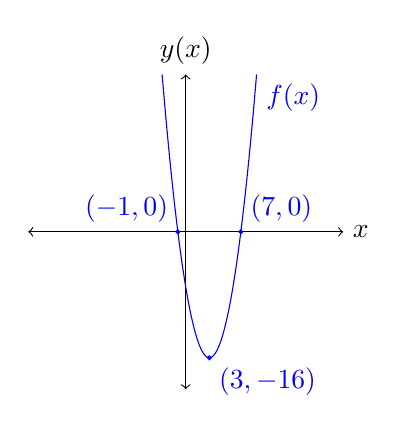
\begin{tikzpicture}[xscale=0.10,yscale=0.10]
      \draw[<->] (-20,0) -- (20,0) node[right] {$x$};
      \draw[<->] (0,-20) -- (0,20) node[above] {$y(x)$};
      \draw[scale=1,domain=-3:9,smooth,variable=\x,blue] plot ({\x},{\x*\x-6*\x-7}) node[below right] {$f(x)$};
      \filldraw[blue] (3,-16) circle[radius=7pt] node[below right] {$(3,-16)$};
      \filldraw[blue] (7,0) circle[radius=7pt] node[above right] {$(7,0)$};
      \filldraw[blue] (-1,0) circle[radius=7pt] node[above left] {$(-1,0)$};
    \end{tikzpicture}
    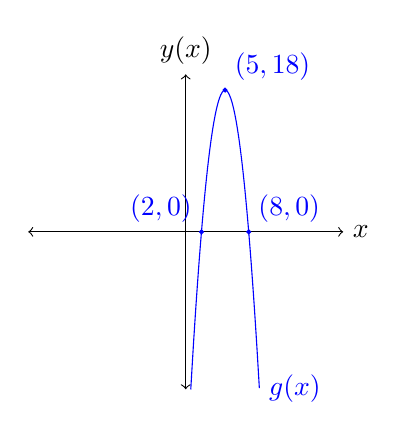
\begin{tikzpicture}[xscale=0.10,yscale=0.10]
      \draw[<->] (-20,0) -- (20,0) node[right] {$x$};
      \draw[<->] (0,-20) -- (0,20) node[above] {$y(x)$};
      \draw[scale=1,domain=0.64:9.35,smooth,variable=\x,blue] plot ({\x},{-2*\x*\x+20*\x-32}) node[right] {$g(x)$};
      \filldraw[blue] (5,18) circle[radius=7pt] node[above right] {$(5,18)$};
      \filldraw[blue] (8,0) circle[radius=7pt] node[above right] {$(8,0)$};
      \filldraw[blue] (2,0) circle[radius=7pt] node[above left] {$(2,0)$};
    \end{tikzpicture}
\end{figure}
This was a pretty simple section.  One last skill you should ensure you know is how to find the equation given a graph.  All you need to do is find the $x$-intercepts, then use another point to determine the compression factor (usually the $y$-intercept or the vertex works very well).  The rest of the chapter covers the methods to convert between forms; we begin with converting from factored form to standard form.
\section{Review: Distribution and F.O.I.L.}
\noindent This section solely covers material that was introduced in Algebra I.  Students should be very familiar with the method reviewed in this chapter and should be comfortable applying it in various situations.  Consider an expression in the form $$(a+b)(c+d)$$ where $a,b,c,d\in\mathbb{R}$.  There are two ways to derive this formula - algebraically and geometrically - and we will derive it both ways.  The first method is using the distributive property (like \hyperlink{chapter.3}{Chapter 3}).  If we distribute the $(c+d)$ term to the left side, we get $$(a+b)(c+d)=a(c+d)+b(c+d).$$  

\begin{wrapfigure}{r}{7cm}
    \centering
\begin{tikzpicture}
    \draw[black] (0,0) rectangle ++(5,5);
    \draw[black] (0,0) rectangle ++(4,1);
    \draw[black] (0,0) rectangle ++(5,1);
    \draw[black] (0,0) rectangle ++(4,5);
    \draw[|<->|] (0,5.5) -- node[fill=white,sloped] {$a$} (4,5.5);
    \draw[|<->|] (4,5.5) -- node[fill=white,sloped] {$b$} (5,5.5);
    \draw[|<->|] (-0.5,1) -- node[fill=white,sloped,rotate=270] {$c$} (-0.5,5);
    \draw[|<->|] (-0.5,0) -- node[fill=white,sloped,rotate=270] {$d$} (-0.5,1);
    \node at (2,0.5) {$ad$};
    \node at (4.5,0.5) {$bd$};
    \node at (2,3) {$ac$};
    \node at (4.5,3) {$bc$};
\end{tikzpicture}
\end{wrapfigure}

Then, use the distributive property to split it.  $$a(c+d)+b(c+d)=ac+ad+bc+bd.$$  That's the split form!  Now let's try the geometric method.  Consider the figure to the right where the area of each rectangle was marked inside.  If we find the area of the largest rectangle, we get the area as $(a+b)(c+d)$.  Adding up the smaller areas, we get $ac+ad+bc+bd$.  This must mean that $$(a+b)(c+d)=ac+ad+bc+bd.$$  This is what we got then first time!

\begin{remark}
Again, like most of the ideas or formulas we derive, don't memorize it.  It's not beneficial; it's much better to understand how to apply it and its derivation.
\end{remark}

This brings what we call the F.O.I.L.  method for multiplying two binomial expressions.  FOIL is an acronym that stands for "First, Outer, Inner, Last" which reminds students how to multiply the binomials.  Let's try a few examples to make sure that we understand the acronym and how it works.
\begin{example}
Expand $(x-2)(x+3)$.
\end{example}
\begin{solution}
Following FOIL, we multiply the first terms ($x\cdot x=x^2$), the outer terms ($x\cdot 3=3x$), the inner terms ($-2\cdot x=-2x$) and the last terms ($-2 \cdot 3=-6$).  Then, adding them up we get $$x^2+3x-2x-6 \implies x^2+x-6.$$ $\Box$
\end{solution}
\begin{example}
Expand $(2x+3)(1-x)$.
\end{example}
\begin{solution}
Following FOIL, we get $2x-2x^2+3-3x=-2x^2-x+3$.$\Box$
\end{solution}
\noindent This section is super short because we just wanted to cover this topic.  We now will move on to special types of quadratics and their properties.
\section{Special Quadratics}
\noindent This section will cover the properties of two special types of quadratics.  We've already seen one of them; we just haven't given it a formal name nor explored it in more detail.

The first special quadratic is the \textit{perfect square trinomial}.  Look at the definition below.
\begin{definition}{Perfect Square Trinomials}{pst}
A perfect square trinomial is defined that, for some real functions $a$ and $b$, $$(a\pm b)^2=a^2\pm 2ab+b^2.$$
\end{definition}
We've done a few examples with these in previous sections.  This is super easy to prove using FOIL, so we challenge you to try this for yourself.  Let's look at a few distribution and factoring examples.
\begin{example}
Expand $(2x-3)^2$.
\end{example}
\begin{solution}
You can either use the formula or use FOIL.  Either way, it produces the same result.  Following the formula, we get $(2x)^2-2(2)(3)+(3)^2=4x^2-12x+9$.  $\Box$
\end{solution}
\begin{example}
Factor $49x^2+28x+4$.
\end{example}
\begin{solution}
All we need to do is follow the definition in reverse.  We see that $49x^2+28x+4=(7x)^2+2(7)(2)+(2)^2=(7x+2)^2$.  $\Box$
\end{solution}
The second special quadratic is the \textit{difference of squares}.  Look at the definition below.
\begin{definition}{Difference of Squares}{dos}
The difference of squares is defined that, for some real functions $a$ and $b$, $$a^2-b^2=(a+b)(a-b).$$
\end{definition}
We haven't seen this example yet, so we will prove it.  There are two ways of proving this: algebraically and geometrically.  The algebraic method involves proving it using FOIL.  All we need to do is expand the right side of the equation.  $$(a-b)(a+b)=a^2+ab-ab-b^2=a^2-b^2.$$
The second way of proving this is geometrically.  Imagine a square with length $a$ where we cut off a slice of length $b$, as seen in the first figure.  We then attach it to the other side to produce the second figure.

\begin{figure}[!h]
    \centering
    \begin{tikzpicture}[xscale=0.5,yscale=0.5]
      \draw (-3,-3) rectangle (3,3);
      \draw[dashdotted] (-3,-2) -- (3,-2);
      \draw[|<->|] (-3,3.75) -- node[fill=white,sloped] {$a$} (3,3.75); 
      \draw[|<->|] (-3.75,-3) -- node[fill=white,sloped] {$b$} (-3.75,-2);
    \end{tikzpicture} $\Longrightarrow$  
    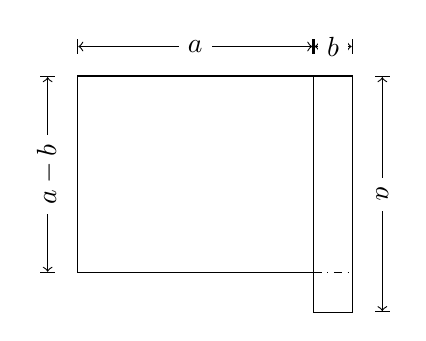
\begin{tikzpicture}[xscale=0.5,yscale=0.5]
      \draw (-3,-2) rectangle (3,3);
      \draw (3,-3) rectangle (4,3);
      \draw[|<->|] (-3,3.75) -- node[fill=white,sloped] {$a$} (3,3.75); 
      \draw[|<->|] (3,3.75) -- node[fill=white,sloped] {$b$} (4,3.75);
      \draw[|<->|] (-3.75,-2) -- node[fill=white,sloped] {$a-b$} (-3.75,3);
      \draw[|<->|] (4.75,-3) -- node[fill=white,sloped,rotate=180] {$a$} (4.75,3);
      \draw[dashdotted] (3,-2) -- (4,-2);
    \end{tikzpicture}   
\end{figure}

We then find the area of each figure.  The area of the first figure is $a^2$ as it is a square.  The area of the second square can be done in parts.  To get the formula we want, we will divide it into the entire upper rectangle and the small square on the bottom (as separated by the dashed line).  The area of this is $(a+b)(a-b)+b^2$.  These should be equal, meaning $$a^2=(a+b)(a-b)+b^2 \implies a^2-b^2=(a+b)(a-b).$$
As we can see, this is the formula in the definition box, so we know we have it correct.

Now, let's try a few examples of this to ensure we understand how use it.
\begin{example}
Distribute $(2x-3)(2x+3)$.
\end{example}
\begin{solution}
Following the formula, we know that the expanded form is $(2x)^2-(3)^2=4x^2-9$.  $\Box$
\end{solution}
\begin{example}
Factor $63x^2-175$.
\end{example}
\begin{solution}
Factor out the common factor of $7$.  This gives $7(9x^2-25)$, which factors to $7(3x-5)(3x+5)$.$\Box$ 
\end{solution} 
This is all we needed to cover regarding these.  We simply wanted to ensure you were aware of these special forms so you can use them to your advantage.  Now, let's discuss one of the toughest sections in this chapter: factoring.
\section{Factoring Standard-Form Quadratics}
\noindent This may be one of the tougher sections of this chapter and is definitely the most difficult to teach.  There are many ways to factor quadratics, where some are more efficient than others.  In this process, we will disregard any factoring method you may know and discuss the methods we find to be most effective.  

There are three methods in this section, where each method builds on another.  It is very important you understand the previous methods as you move on to the more difficult, as they become more difficult to understand and more intuitive.  We outline each method in its own subsection; it is imperative that you attempt each problem on your own before reviewing the solution.
\subsection{Splitting the Middle Term}
\noindent This is the most common factoring technique that used to be taught in schools.  Schools now are using a visual factoring method that we find to be a waste of time and space.  Splitting the middle term offers the best value for the time spent learning and practicing, which makes it a good investment.

The goal of splitting the middle term (and every other method) is to find two numbers that multiply to the constant term and add to the linear term.  The derivation for this is explained in the \hyperlink{section.5.5.2}{next} subsection.  Once we do this, we "split" the middle term into these two factors and the \textit{factor by grouping}.  Let's try this.
\begin{example}
Factor $x^2+6x+8=0$.
\end{example}
\begin{solution}
We need two numbers that multiply to $8$ and add to $6$.  Let's consider the factors of $8$: $1$, $2$, $4$, and $8$.  Right away we see that $2+4=6$.  To split the middle term, we simply rewrite the function as $x^2+\left(2x+4x\right)+8$.  Now, we factor by grouping.  To do this, we simply find the greatest common factor of the first two terms and of the last two terms.  This looks like $$x^2+2x+4x+8=x(x+2)+4(x+2).$$  We then factor the $(x+2)$ from both terms to get $$x(x+2)+4(x+2)=(x+4)(x+2).$$ $\Box$
\end{solution}
Let's add some negatives to the problem to see how it changes the way we look at it.
\begin{example}
Factor $x^2-3x-10=0$.
\end{example}
\begin{solution}
We need two numbers that multiply to $-10$ and add to $-3$.  We know that these two numbers must have opposite signs and that the larger number must be negative.  The factors of $10$ are $1$, $2$, $5$, and $10$, and the pair that works is $-5$ and $2$.  Splitting the middle term, we get $$x^2-5x+2x-10=0.$$  Factoring by grouping gives $$x(x-5)+2(x-5) \implies (x+2)(x-5)=0.$$ $\Box$
\end{solution}
What happens when $a\neq 1$?  The problem doesn't become so easy.  We do have a method for this; however, that makes it seem as easy as this first type of problem.  We will use the method of bringing the leading coefficient to the back and factor as normal.
\begin{example}
Factor $2x^2+5x-3=0$.
\end{example}
\begin{solution}
If we bring the leading coefficient ($2$) to the back, we get the new equation $x^2+5x-6=0$.  This is something we know how to factor!  We look for two numbers that multiply to $-6$ and add to $5$.  Considering the factors of $6$, we have $1$, $2$, $3$, and $6$.  The factor pair that adds to $5$ when the pair has opposite signs is $6$ and $-1$ (Do not fall for the $2$ \& $3$ pair trap!)  Splitting the middle term, we get $$x^2+6x-x-6=0 \implies x(x+6)-(x+6)=0 \implies (x+6)(x-1)=0.$$  

But we're not done!  Note that you don't get the original equation if you FOIL our solution.  Essentially, we multiplied the constant term by 2 in order to factor it; thus, we need to divide the constants by $2$.  This gives $$\left(x+3\right)\left(x-\dfrac{1}{2}\right)=0.$$  Instead of writing the second term like this, we move the $2$ to the $x$ term and the root doesn't change (be sure you see why).  This gives the factors $$(x+3)(2x-1)=0.$$ $\Box$
\end{solution}
The only time that this method is ineffective is when the values of $a$, $b$, and $c$ are large; there would be a lot of factors to go through.  This is best dealt with in the next section when we discuss factoring via coefficients.
\subsection{Factoring via Coefficients}
\noindent This is a tough method to learn.  It involves solving simple systems of equations by understanding a little about number theory.  This method, along with the next one, require a great deal of number sense with respect to divisibility, multiplication of (sometimes large) numbers, and factors of commonly seen numbers.

Let's try and derive the ideas we will need in this section.  Given two roots of a polynomial, $\lambda_1$ and $\lambda_2$, we know that the quadratic must be in the form $$(x+\lambda_1)(x+\lambda_2)=x^2+\left(\lambda_1+\lambda_2\right)x+\lambda_1\lambda_2.$$  That means, we know that we have a system of equations here.  If $f(x)=x^2+bx+c$ (assuming $a=1$), we know that $\lambda_1+\lambda_2=b$ and $\lambda_1\lambda_2=c$.  To factor the quadratic, we need to solve for $\lambda_1$ and $\lambda_2$.  We aren't going to find a solution in terms of $b$ and $c$; instead we will find a solution case-by-case.

Let's try a few examples to get the hang of this idea.
\begin{example}
Factor $x^2-13x+36=0$.
\end{example}
\begin{solution}
We know that $\lambda_1+\lambda_2=-13$ and $\lambda_1\lambda-2=36$.  Because $\lambda_1\lambda_2>0$, $\lambda_1$ and $\lambda_2$ have the same sign, and since $\lambda_1+\lambda_2<0$, we know that $\lambda_1$ and $\lambda_2$ are both negative.

Consider the factors of $36$.  We have $(1,36)$, $(2,18)$, $(3,12)$, $(4,9)$, and $(6,6)$.  The $(4,9)$ pair is the only pair that adds to $13$, so our factors are $(x-4)(x-9)$.  $\Box$ 
\end{solution}
\begin{example}
Find the roots of $x^2-12x-540=0$.
\end{example}
\begin{solution}
The numbers just got much bigger.  We know that $\lambda_1\lambda_2=-540$ and $\lambda_1+\lambda_2=-12$.  Since $\lambda_1\lambda_2<0$, we know that $\lambda_1$ and $\lambda_2$ have different signs.  Since $\lambda_1+\lambda_2<0$, the larger number must be negative.  Since $540$ has $12$ pairs of factors, and we don't want to go through all these factors, we will find an alternate solution.

Let's determine if $\lambda_1$ and $\lambda_2$ have any common factors.  We first note that $12$, $540$, and $0$ are all even.  If $x$ is odd, then the quadratic is odd and thus can't equal zero (be sure to check this for yourself).  This means that the roots are even.

We also note that $12$, $540$, and $0$ are divisible by three.  Using the same logic as the previous paragraph, we know that the roots must be divisible by $3$.

Using basic divisibility rules, we know that the roots must be divisible by $6$ as well.  We then define new roots, $\mu_1$ and $\mu_2$, such that $6\mu_1=\lambda_1$ and $6\mu_2=\lambda_2$.  This means that $6\mu_1+6\mu_2=-12$, so $\mu_1+\mu_2=-2$.  Also, $\left(6\mu_1\right)\left(6\mu_2\right)=-540$, so $\mu_1\mu_2=-15$.  This is much easier to solve.  We quickly see that $\mu_1=-5$ and $\mu_2=3$, meaning that $\lambda_1=-30 $ and $\lambda_2=18$.  Thus, our factors are $$x^2-12x-540=(x+18)(x-30)=0,$$ meaning that $x_1=-18$ and $x_2=30$.  $\Box$
\end{solution}
Up until now, we've only dealt with cases where $a=1$.  What if $a\neq 1$?  Can we write the same equations?  The short answer is: no.  Let's look at an example where this applies.
\begin{example}
Factor $3x^2+11x+10=0$.  
\end{example}
\begin{solution}
In this case, $a=3$.  This problem is slightly easier since $3$ is prime; it means there's only one pair that works: $3x\cdot x=3x^2$.  This means we write the factors as $(3x+\lambda_1)(x+\lambda_2)$.  FOILing this gives $$(3x+\lambda_1)(x+\lambda_2)=3x^2+(\lambda_1+3\lambda_2)x+\lambda_1\lambda_2.$$  So, we need to find values for $\lambda_1$ and $\lambda_2$ that satisfy $\lambda_1+3\lambda_2=11$ and $\lambda_1\lambda_2=10$.  The factor pairs of $10$ are $(1,10)$, $(2,5)$, $(5,2)$, and $(10,1)$.  Unlike Example 5.20, the order does matter here because of the different coefficients on $x$.  The only factor pair that works here is $(5,2)$, meaning $3x^2+11x+10=(x+5)(x+2)$.  $\Box$
\end{solution}
Now, what if $a$ isn't prime?  This means we need to introduce two new variables into the equation.
\begin{example}
Factor $9x^2+88x-20=0$.
\end{example}
\begin{solution}
In this case, $a=9$ has three factor pairs ($(1,9)$, $(3,3)$, and $(9,1)$).  So, we introduce two new variables $\mu_1$ and $\mu_2$ to represent that coefficient.  Thus, the factors are $(\mu_1x+\lambda_1)(\mu_2x+\lambda_2)$.  This expands to $$(\mu_1x+\lambda_1)(\mu_2x+\lambda_2)=(\mu_1\mu_2)x^2+\left(\mu_1\lambda_2+\mu_2\lambda_1\right)x+\lambda_1\lambda_2.$$
This gives the system of equations $\mu_1\mu_2=9$, $\mu_1\lambda_2+\mu_2\lambda_1=88$, and $\lambda_1\lambda_2=-20$.  But wait!  This is a four variable, three equation system.  This isn't possible!  There is a fourth restriction though - each variable must be an integer.

Let's consider this solution logically.  $88$ is a very big positive number.  $\lambda_1\lambda_2<0$, meaning that either $\lambda_1$ or $\lambda_2$ is negative.  We quickly deduce that $\lambda_1$ must be a (small) negative number.  We know that both $\mu_1$ and $\mu_2$ must be positive for this to work, and must have a significant size difference.  Let $\mu_1=9$ and $\mu_2=1$.  This means that $9\lambda_2+\lambda_1=88$.  The only solution that works here is $\lambda_1=-2$ and $\lambda_2=10$.  

Thus, our factors are $(9x-2)(x+10)$.  $\Box$
\end{solution}
These are the different types of coefficient factoring.  Let's move on to intuitive factoring, a more mental solution that combines the last two methods.
\subsection{Intuitive Factoring}
\noindent This section is undoubtedly the hardest to teach, the hardest to learn, the one that requires the most practice, yet the most rewarding.  Once you understand how to use it, you will be factoring at lightning speeds with amazing accuracy.  Essentially, this method is the previous one without showing as much work nor thinking as hard.

This method is more like the first method as it looks for the numbers that multiply to the constant and add to the linear term.  However, this method can be used for larger values of $a$, $b$, and $c$ without too much difficulty.

Let's try a few examples of this that cover various cases of intuitive factoring.
\begin{example}
Factor $x^2-x-12=0$.
\end{example}
\begin{solution}
We need two numbers that multiply to $-12$ and add to $-1$.  Instead of listing every factor, let's consider the solution intuitively.  The numbers we need must have opposite sign and the larger must be negative.  We also know they are close in magnitude, since their sum is near zero.  So, we look for two factors near $\sqrt{12}\approx 3.5$ (be sure you know why!).  The two factors that work here are $-4$ and $3$, so our factors are $(x-4)(x+3)$.  $\Box$
\end{solution}
\begin{example}
Factor $x^2-7x-18=0$.
\end{example}
\begin{solution}
We need two numbers that multiply to $-18$ and add to $-7$.  We know that they must be of opposite sign and should have a somewhat-large difference.  We also know that the larger number must be negative.  Since the linear term is near half the constant term, we should look for a root around $2$ and the corresponding roots (in this case $-9$).  We see that $-9$ and $2$ works, so the factors are $(x-9)(x+2)=0$.$\Box$
\end{solution}
Let's move on to a few examples where $a\neq 1$.
\begin{example}
Factor $2x^2-17x+35=0$.  
\end{example}
\begin{solution}
The number are getting slowly bigger and now there's a leading coefficient.  Since $2$ is prime, the only way to use it is $(2x+\lambda_1)(x+\lambda_2)$.  Since $35$ is positive, the numbers must have the same (negative) sign.  Again, since the difference between the coefficients of $x$ is low, and since the linear term is about half the constant term, the constants will be approximately equal.  The smaller of the two constants will usually be multiplied by the higher $x$-coefficient.  We pick $-5$ and $-7$ as the factors of $35$ and note that $(2)(-5)+(1)(-7)=-17$.  When you multiply these terms, according to FOIL, we put them in the \textbf{opposite} factor.  So, the factors become $(2x-7)(x-5)=0$.  $\Box$
\end{solution}
\begin{remark}
  This problem can also be solved by bringing $2$ to the back and factoring as usual.  We will do this in the next example.
\end{remark}
This last one was probably tough to follow.  Again, this method is not easy.  But once you understand a bit of the number theory behind it, it becomes a lot easier.

Let's try one where $a$ isn't prime.
\begin{example}
Factor $6x^2+11x-10$.
\end{example}
\begin{solution}
Since $a$ isn't prime, and there's not a good way to deal with this, we bring it to the back.  This gives $x^2+11x-60=0$.  Since the middle term is approximately a quarter of the constant term, we try the roots $15$ and $-4$.  They work!  This gives the factors $(x+15)(x-4)=0$.  We then divide the constants by $6$ to get $$(x+15)(x-4)\implies \left(x+\dfrac{5}{2}\right)\left(x-\dfrac{2}{3}\right)\implies (2x+5)(3x-2)=0.$$ $\Box$
\end{solution}
These are the essentials of intuitive factoring.  Continue to practice it as we move on to hidden quadratics, where we find secret quadratics inside of seemingly impossible functions.
\section{Hidden Quadratics}
\noindent The goal of this section is to learn to factor "hidden" quadratics.  Hidden quadratics are quadratic functions where the $x$-variable is some other function, such as an exponential, trigonometric, or other.  All we need to do is make a substitution to make the quadratic into a function we know how to factor and solve it.

Let's look at a few examples to understand how to solve it.  
\begin{example}
Solve $\left(3^x\right)^2-12\left(3^x\right)+27=0$.
\end{example}
\begin{solution}
We see that we almost have a quadratic if it weren't for the $3^x$ terms.  So, we make what's known as a \textbf{u-substitution}.  In this case, we let $u=3^x$.  Why?  This will help us to remove both $3^x$ terms and leave a quadratic!
$$\left(3^x\right)^2-12\left(3^x\right)+27=0 \implies u^2-12u+27=0.$$  We know how to solve the resultant equation.  Let's factor it.  $$u^2-12u+27=u^2-3u-9u+27=u(u-3)-9(u-3)=(u-3)(u-9)=0.$$
Using the zero-product property, we know that $u=3$ and $u=9$.  But we're not done!  Recall that the original equation was in terms of $x$, not $u$.  This means that we have to re-substitute the value of $u$ for $3^x$ to solve for $x$.  This means that we have $3^x=3$ and $3^x=9$, which we know is $x_1=1$ and $x_2=2$.  $\Box$
\end{solution}
The important part of this section is ensuring that you re-substitute the value of $u$ for $x$.  In the next example, we are going to factor the quadratic without making the substitution.
\begin{example}
Solve $3\left(3^x\right)^2-4\left(3^x\right)+1=0$.
\end{example}
\begin{solution}
Without making the substitution, we need to factor.  We only are going to consider the coefficients as it's a hidden quadratic in standard form.  Remembering the second type of factoring we learned, where we move the leading coefficient "to the back", we get the factors to be $\left(3\cdot 3^x-1\right)\left(3^x-1\right)=0.$  This means that $3^x=\dfrac{1}{3}$ and $3^x=1$.  Thus, $x_1=-1$ and $x_2=0$.  $\Box$
\end{solution}
The last type of problem we need to cover is if one of the resultant solutions doesn't exist.  This may happen due to domain and range restrictions on the $u$-function.
\begin{example}
Solve $\left(3^x\right)^2-9\left(3^x\right)-22=0$.  You may use a scientific calculator; round your answer to two digits.
\end{example}
\begin{solution}
Let $u=3^x$.  This means that $u^2-9u-22=0$.  Factoring gives $(u-11)(u+2)=0$, meaning $u_1=-2$ and $u_2=11$.  Re-substituting, we get $3^x=-2$ and $3^x=11$.  Since $3^x\neq -2$ since the range of $f(x)=3^x$ is $y>0$.  This leaves $3^x=11$.  We don't have a great way of solving this.  Using some trial and error to find a close answer, we get $x=2.18$.  $\Box$
\end{solution}
Note that we used $3^x$ for every problem.  There are an infinite number of values for $u$ that will be used, but without covering other types of functions, it's hard to have a variety.  A bit more variety is put in the problem sets.

Those are the three main types of hidden quadratic expressions.  Now, let's move on to a new method of conversion: completing the square (converting from standard to vertex form).
\section{Completing the Square}
\noindent The next method of solving quadratic equations is to \textit{complete the square}.  The goal of this method is to "factor" it in such a way that $x$ is only in one term.  The achieved form of this quadratic is known as the \textit{vertex form}.  Thus, our goal is to change the form of the quadratic from $$a_1x^2+a_2x_+a_3\longrightarrow a(x+x_0)^2+y_0.$$
We are going to attempt to derive this in terms of generic constants ($a_1$, $a_2$, and $a_3$).  The first thing we need to do is separate the $x$ terms by factoring out an $a_1$ from \textit{only} the first two terms, thus: $$a_1x^2+a_2x+a_3=a_1\left(x^2+\frac{a_2}{a_1}x\right)+a_3.$$  Now, we need to find a way to make the polynomial inside the parentheses to a perfect square.  We know that the perfect square of a monomial is in the form $$(x+m)^2=x^2+(2m)x+m^2.$$  Thus, to find $m^2$, we need to \textit{divide the middle term by two and square it}.

Our middle term is $\displaystyle \frac{a_2}{a_1}$.  Following the process explained above, we get that the last term is $\displaystyle \frac{a_2}{a_1} \implies \frac{a_2}{2a_1} \implies \frac{a_2^2}{4a_1^2}$.  So we must add this to the inside to get the perfect square polynomial; however, what we do to one side, we must do to another.  To ensure that the equation is balanced, we will subtract this value outside the parentheses.  Note that the parentheses is being multiplied by $a_1$, so we must account for that outside:
$$a_1\left(x^2+\frac{a_2}{a_1}x+\frac{a_2^2}{4a_1^2}\right)+a_3-\left(a_1\right)\left(\frac{a^2}{4a_1^2}\right)=a_1\left(x^2+\frac{a_2}{a_1}x+\frac{a_2^2}{4a_1^2}\right)+\left(a_3-\frac{a_2^2}{4a_1}\right).$$
All we need to do is write the inside as a perfect square.  This isn't too difficult:
$$y(x)=a_1\left(x+\frac{a_2}{2a_1}\right)^2+\left(a_3-\frac{a_2^2}{4a_1}\right)$$
In this form, $\displaystyle x_0=\frac{a_2}{2a_1}$ and $\displaystyle y_0=a_3-\frac{a_2^2}{4a_1}$.  Note the following remark:

\begin{remark}
  Do NOT memorize this formula.  There is no benefit to doing this.  Work out each problem individually and understand the process.
\end{remark}

There are two important applications for completing the square: $(1)$ for solving a quadratic equation, and $(2)$ for graphing a quadratic function.  We will cover graphing in \hyperlink{section.5.9}{Section 5.9}.  Let's look at a few examples to demonstrate mastery of the process:
\begin{example}
Write the following in vertex form: $y(x)=x^2+3x+1$.
\end{example}
\begin{solution}
There is nothing to factor out of the first two terms.  The term that needs to be added/subtracted is $\displaystyle \left(\frac{3}{2}\right)^2=\frac{9}{4}$.  We get the vertex form of the polynomial as $$y(x)=\left(x^2+3x+\frac{9}{4}\right)+1-\left(1\right)\left(\frac{9}{4}\right)=\left(x+\frac{3}{2}\right)^2-\frac{5}{4}.$$$\Box$
\end{solution}
\begin{example}
Solve the following quadratic equation via completing the square: $x^2+4x-5=0$.
\end{example}
\begin{solution}
Since there's nothing to factor, we find the added term to be $\displaystyle \left(\frac{4}{2}\right)^2=4$.  This makes the completed square $$\left(x^2+4x+4\right)-5-4=(x+2)^2-9=0.$$  All we need to do is solve it for $x$, which is fairly easy.  Adding $9$ to both sides, we get $(x+2)^2=9$.  Taking the square root of both sides gives $x+2=-3$ and $x+2=3$, meaning that $x=-5$ and $x=1$.$\Box$
\end{solution}
\noindent Now, let's move on to the final method of solving a quadratic equation: the quadratic formula.
\section{The Quadratic Formula}
\noindent After covering all the other factoring types, we arrive at the final types of quadratics: the ones that can't be factored.  As a result, we are tasked to find a formula that can solve the quadratic for $x$ given any coefficients of the polynomial.  We will consider the standard polynomial $y(x)=ax^2+bx+c$, where $a,b,c\in\mathbb{R}$.  We are going to solve for $x$ by completing the square; we did a very similar derivation in \hyperlink{section.5.7}{Section 5.7}, so we won't do too much explaining.  Let's complete the square:
$$y(x)=ax^2+bx+c=a\left(x^2+\frac{b}{a}x\right)+c=a\left(x^2+\frac{b}{a}x+\frac{b^2}{4a^2}\right)+c-\frac{b^2}{4a}$$
We will combine the constant terms into a singular fraction.  Remember that, since we are trying to find the roots of the polynomial, we need to let $y(x)=0$.
$$0=a\left(x+\frac{b}{2a}\right)^2+\frac{4ac-b^2}{4a} \implies a\left(x+\frac{b}{2a}\right)^2=\frac{b^2-4ac}{4a} \implies \left(x+\frac{b}{2a}\right)^2=\frac{b^2-4ac}{4a^2}$$
We need to take the square root of both sides.  Remember that both roots - not just the principal root - are important.  We will denote both roots using a "$\pm$".  Note that you could use an absolute value; however, the final formula looks a little cleaner and is more well-known this way.
$$x+\frac{b}{2a}=\frac{\pm\sqrt{b^2-4ac}}{2a} \implies x=\frac{-b\pm\sqrt{b^2-4ac}}{2a}$$
There it is.  That's the quadratic formula.  Sure, it's not the prettiest formula in the world.  Let's emphasize it in the definition below.
\begin{definition}{The Quadratic Formula}{quadform}
Given a quadratic polynomial $y(x)=ax^2+bx+c$, where $a,b,c\in\mathbb{R}$ and $a\neq 0$, the roots of the polynomial can be expressed as $$x=\frac{-b\pm\sqrt{b^2-4ac}}{2a}.$$
The value inside the square root, known as the \underline{discriminant}, determines the classifications of solutions.
\end{definition}
\begin{remark}
  Unlike the complete the square formula, this is an essential formula to memorize.  The more you use it, the easier it gets to memorize!
\end{remark}
There are three categories of the discriminant (symbol: $\Delta$): When $\Delta>0$, $\Delta=0$, and $\Delta<0$.  Now, let's consider each type: \begin{enumerate}
    \item If $\Delta>0$, this means that the square root will be a real value; due to the $\pm$, there will be \textbf{two distinct real solutions}.
    \item If $\Delta=0$, this means that the square root will be zero, nullifying the $\pm$.  This yields \textbf{one repeated real solution}.
    \item If $\Delta<0$, this means that the square root will be negative, giving \textbf{two complex conjugate solutions}.
\end{enumerate}
Let's consider an example of each type:
\begin{example}
Solve the following quadratic equation: $2x^2+x-28=0$.
\end{example}
\begin{solution}
Since $a=2$, $b=1$, and $c=-28$, we get $$x=\frac{-(1)\pm\sqrt{(1)^2-4(2)(-28)}}{2(2)}=\frac{-1\pm\sqrt{225}}{4}=\frac{-1\pm 15}{2}\implies \begin{matrix} x_1=-8 \\ x_2=7 \end{matrix}.$$$\Box$
\end{solution}
\begin{example}
Solve the following quadratic equation: $x^2-8x+16=0$.
\end{example}
\begin{solution}
Since $a=1$, $b=-8$, and $c=16$, we get $$x=\frac{-(-8)\pm\sqrt{(-8)^2-4(1)(16)}}{2(1)}=\frac{8\pm 0}{2} \implies x_{1,2}=4.$$ $\Box$
\end{solution}
\begin{example}
Solve the following quadratic equation: $x^2+2x+4=0$.
\end{example}
\begin{solution}
$$x=\frac{-(2)\pm\sqrt{(2)^2-4(1)(4)}}{2(1)}=\frac{-2\pm\sqrt{-12}}{2}=\frac{-2\pm 2i\sqrt{3}}{2} \implies \begin{matrix} x_1=-1-i\sqrt{3} \\ x_2=-1+i\sqrt{3} \end{matrix}.$$ $\Box$
\end{solution}
\noindent There isn't much else to cover regarding the quadratic formula.  It's super straight-forward and there's no other variability to it.  Now, let's discuss the final, and possibly the most important, section of the chapter: graphing quadratics.
\section{Summary of Quadratics}
This section plans to cover no new material; the goal of this section is to bring all the information from this chapter together to ensure that you got everything out of the chapter that you will need.

The big piece of information to take away from this section is the method to convert between forms.  The next three paragraphs explain the basic process (and/or name) to convert between each form.

Let's start with standard form.  To get from standard form to vertex form, you complete the square (\hyperlink{section.5.7}{5.7}).  To get to factored form, you simply factor (\hyperlink{section.5.5}{5.5}).

Then, we move to vertex form.  To get to standard form, distribute the squared term and combine the constants.  To get to factored form, you can use difference of squares (\hyperlink{section.5.6}{5.6}).  Otherwise, convert to standard form and factor.

Last, we look at factored form.  To get to standard form, FOIL the factors.  To get to vertex form, take the average of the intercepts to get the $x$-coordinate of the vertex, then just find the $y$-coordinate from there.  Sometimes, it might be easier to go to standard form then complete the square.

Note that its often easier to go to standard form first to get between vertex form and factored form.  Sometimes it might be easier to go straight between them, but using standard form is always an option.

\begin{reviewset}
\item Find the domain of $f(x)=\dfrac{x-7}{\dfrac{1}{x}+\dfrac{1}{x^2+6}}.$ \vspace{2mm}
\item For the following equations, solve for $x$.  \newline
(a) $x^2+12x+27=0$ \hspace{48mm} (b) $x^2-6x+1=0$ \newline 
(c) $2x^2-5x+2=0$ \hspace{50mm} (d) $3x^2=7-15x$ \vspace{2mm}
\item Let $f$ be defined such that $f(x/2)=x^2+x+1$.  Find the sum of the values of $s$ such that $f(2s)=7$.  \vspace{2mm}
\item Given that one root of $2x^2+rx+s=0$, with $r$ and $s$ as real numbers, is $3+2i$.  Find $s$.  \vspace{2mm}
\item For each problem, graph the quadratic by completing the square.  \newline 
(a) $f(x)=x^2+6x+13$ \hspace{49mm}
(b) $g(x)=3x^2-6x+5$ \newline
(c) $h(x)=2x^2+8x+6$ \hspace{49mm}
(d) $j(x)=3x^2+x-1$ \vspace{2mm}
\item The sum of the squares of the roots of $x^2+2hx-3=0$ is $10$.  Find $|h|$.  \vspace{2mm}
\item Given the pieces of information below, write a quadratic function.  Then, convert it into all forms.  \newline 
(a) A quadratic with vertex at $(2,3)$ and a $y$-intercept of $(0,1)$.  \newline 
(b) A standard quadratic with roots at $x=-4$ and $x=1$.  \newline
(c) An inverted quadratic with $y$-intercept at $(0,2)$, compression factor of $|a|=\dfrac{1}{2}$, and contains $(5,2)$.  [$\star$] \vspace{2mm}
\item Find the roots of $x^2+\left(a-\dfrac{1}{a}\right)x-1=0$ in terms of $a$.  \vspace{2mm}
\end{reviewset}
\begin{challengeset}
\item Let $a$ and $b$ be the roots of the equation $x^2-mx+2=0$.  Suppose that $a+\dfrac{1}{b}$ and $b+\dfrac{1}{a}$ are the roots of the equation $x^2-px+q=0$.  What is $q$? (IMPORTANT: For a polynomial $ax^2+bx+c=0$ with real constants $a$, $b$, and $c$, then the product of the roots is $\dfrac{c}{a}$.) \vspace{2mm}
\item One of the roots of $x^2-ax+2a+3=0$ is three times the other.  Find all possible values of $a$.  (IMPORTANT: For a polynomial $ax^2+bx+c=0$ with real constants $a$, $b$, and $c$, then the sum of the roots is $-\dfrac{b}{a}$.) \vspace{2mm}
\item Find the positive difference of the roots of $x^2-rx+\dfrac{r^2-1}{4}=0$.  \vspace{3mm}
\item Solve $\sqrt{4x^2+20x+25}=2x+5$.  \vspace{2mm}
\item Solve $4^x+2^{x+2}-32=0$ for $x$.  \vspace{2mm}
\item Find all values of $x$ such that $\left(x^2-5x+5\right)^{(x^2-9x+20)}=1$.  \vspace{3mm}
\item Find all ordered pairs $(x,y)$ that satisfy both $x^2-xy=10$ and $xy+y^2=6$.  (HINT: try to combine them in some way; what comes of it?) \vspace{2mm}
\item Let $P(x)$ be a polynomial such that $P(0)=-1$, $P(1)=9$, and $P(2)=25$.  Find $P(-1)$.  \vspace{2mm}
\end{challengeset}
\begin{remark}
  The two notes given in Problems 1 and 2 of the challenge set are a part of a series of formulas known as \textit{Vieta's Formulas}.  They will be covered in Pre-calculus.
\end{remark}
%%%%%%%%%%%%%%%%%%%%%%%%%%%%%% CHAPTER 6 %%%%%%%%%%%%%%%%%%%%%%%%%%%%%%%%%%%%%%%%%%%%%
\chapter{Higher-Order Polynomials}
\begin{introduction}[Contents]
\item Theory of Graphing Higher-Order Polynomials
\item Theory in Solving Higher-Order Polynomials, Part I
\item Theory in Solving Higher-Order Polynomials, Part II
\item The Special Cases
\item Graphing Polynomial Functions
\end{introduction}
\noindent A polynomial is an expression in the form $$P(x)=a_0+a_1x+a_2x^2+a_3x^3+\ldots+a_nx^n$$ for some real constants $a_1$,$a_2$,$a_3$,$\ldots$,$a_n$.  We define polynomials by their \textit{degree}, which is considered to be the highest power of the polynomial (for example, a quadratic has degree $2$).

We then can name the polynomial based on its degree; a polynomial of the third degree is considered a \textit{cubic}, a fourth-degree polynomial is a \textit{quartic}, and so on.  These first few names are important to be able to identify; after that, we simply use the degree number (i.e seventh-degree polynomial).

The goal of this chapter is to extend the theory of quadratic functions into higher-orders (degrees) and determine various properties associated with them.  Our goal is to see how similar polynomials of different degrees are and how we can predict behavior based on certain aspects of the function.
\section{Basic Theory of Higher-Order Polynomials}
\noindent To begin our discussion of higher order polynomials, we will delve into the various theories that surround them. Now you may be wondering, why are these polynomials different from a normal quadratic or a line? Well, the reason for this is because unlike quadratics or lines, there isn't exactly a guaranteed way to solve for zeros, nor an "easy" way to graph them precisely.  We need to consider a few things about polynomials to help us better understand them and graph them.

We begin with degree.  The definition of a degree was explained in the introduction to the chapter.  The numeric value of the degree is important, but so is whether it is even or odd.  Below are the two rules: \begin{itemize}
    \item If the degree of the polynomial is even, the end behavior is even.  This means that as $x\to-\infty$ and as $x\to\infty$, they will travel in the same direction.  The direction is determined by the sign of the leading coefficient ($a_n$): if $a_n<0$, the shape of the polynomial will go both down ($f(x)\to-\infty$); if $a_n>0$, both ends will go up ($f(x)\to\infty$).
    \item If the degree of the polynomial is odd, the end behavior is odd.  This means that as $x\to-\infty$ and as $x\to\infty$, they will travel in opposite directions.  Again, the direction is determined by the sign of the leading coefficient ($a_n$): if $a_n<0$, the left side ($f(-\infty)\to\infty$ and $f(\infty)\to-\infty$); if $a_n>0$, both ends will go up ($f(-\infty)\to-\infty$ and $f(\infty)\to\infty$).
\end{itemize}
The next thing we need to understand are \textit{extrema}.  Polynomials can have turns in the graph $-$ there can be $n-1$ turns (where $n$ is the degree).  This means that quadratics can have up to $1$ turn (they all do), cubics can have $2$, and so on.  There are two types of extrema: \textit{local extrema} and \textit{global extrema}. Let's explore the difference:
\begin{itemize}
    \item Local extrema are the maximum and minimum of a function in a given interval. For example, many cubic graphs have two turns as seen below.  The local maximum is at the top of the left "crest" and the local minimum is at the bottom of the right "trough".
    \item Global extrema are the highest and lowest points of a function over its entire domain.  For example, on the cubic graph below, we see that the global maximum is $\infty$ and the global minimum is $-\infty$.
\end{itemize}
\begin{figure}[!h]
    \centering
    \hspace{\stretch{1}}
    \begin{tikzpicture}[xscale=0.4,yscale=0.4]
        \draw[<->] (-5,0) -- (5,0) node[right] {$x$};
        \draw[<->] (0,-5) -- (0,5) node[above] {$f(x)$};
        \draw[blue,domain=-2:2] plot ({\x},{\x*\x*\x-2*\x});
    \end{tikzpicture} \hspace{\stretch{1}}
    \begin{tikzpicture}[xscale=0.4,yscale=0.4]
        \draw[<->] (-5,0) -- (5,0) node[right] {$x$};
        \draw[<->] (0,-5) -- (0,5) node[above] {$f(x)$};
        \draw[blue,domain=-1.5:1.5] plot ({\x},{\x*\x*\x*\x});
    \end{tikzpicture} \hspace{\stretch{1}}
\end{figure}
We should note that there's not always $n-1$ turns in the graph.  Consider the graph of $f(x)=x^4$ above, where there is one turning point. So how do we know when there will be a turn? There's not a great method, but we will explore a good method when we discuss finding the roots of a polynomial.

The final theorem to discuss is the \textit{Intermediate Value Theorem}.  

\begin{theorem}{The Intermediate Value Theorem}{intval}
Given a polynomial $f(x)$ that is continuous on the interval $(a,b)$, where $a,b\in\mathbb{R}$ and $a<b$, and if $f(a)<0$ and $f(b)>0$ or vice-versa, then somewhere along this interval, there exists some value of $c$ where $a<c<b$ such that $f(c)=0$.
\end{theorem}

This theorem is really common sense of you think about it. If a function is below the $x$-axis at some point, and further on down the line, it is above, somewhere in between the function had to cross the $x$-axis, provided the function doesn't have any asymptotes or holes or anything. (This, of course, is true in reverse $-$ starting above the $x$-axis.)

This concludes our discussion of theories regarding graphing. You may be wondering; this wasn't that bad? Well for starters, whenever math is easy, it has to get hard. And secondly, why did you jinx it? 

\section{Theory in Solving Higher-Order Polynomials, Part I}
\noindent In this section, we’re going to delve into the theories of solving polynomial equations and inequalities. Now a lingering question may remain from the last section: you showed me how to graph this, but how do I actually figure out things about the function rather than guessing how it looks? We're now going to do just that.

Polynomial equations are often in the form $k=a_0+a_0+a_1x+a_2x^2+a_3x^3+\ldots+a_nx^n$.  We seek to solve functions in the form $f(x)=0$, so we subtract. $$0=(a_0-k)+a_1x+a_2x^2+a_3x^3+\ldots+a_nx^n \implies 0=a_0'+a_1x+a_2x^2+a_3x^3+\ldots+a_nx^n,$$ where $a_0'=a_0-k$.  There are loads of methods to solve these, but in order to hone in on those methods, we need to discuss any attributes of these zeroes first.  First, we want to count how many there are.  Is there a general form for that?

Consider the polynomial $0=1-x+x^2-x^3$. How many solutions should we expect? Well, for a line we expect one solution.  For a quadratic, it has two solutions.  If we extrapolate this to the $n^{\text{th}}$ degree, we make the following conjecture: \textit{A polynomial of degree $n$ has $n$ roots}.  This is actually known as the \textit{Fundamental Theorem of Algebra}. It's pretty common sense, we know. We even put it in a box because it's important.
\begin{theorem}{Fundamental Theorem of Algebra}{fundtheorem}
A polynomial of degree $n$ has $n$ roots.
\end{theorem}

\begin{remark}
Side note, most fundamental theorems are common sense.  Here's another (called the Trivial Inequality): $x^2\geq 0$.
\end{remark}

There's more we can tell about the roots.  Descartes, a renown mathematician and philosopher, created a rule to outline expectations we have for the solutions to the equation.  
\begin{theorem}{Descartes' Rule of Signs}{desc}
Descartes' Rule of Signs predicts how many solutions will be positive, how many will be negative, how many might be real, etc.
\begin{enumerate}
    \item For some polynomial $f(x)$, count the number of sign changes. \begin{itemize}
        \item If the number of sign changes is odd, then there is at least $1$ positive real solution.
        \item If the number of sign changes is even, then there is at least $0$ positive real solutions.
        \end{itemize}
    \item For the polynomial $f(-x)$, count the number of sign changes. \begin{itemize}
        \item If the number of sign changes is odd, then there is at least $1$ negative real solution.
        \item If the number of sign changes is even, then there is at least $0$ negative real solutions.
    \end{itemize}
\end{enumerate}
This will be useful for predicting what roots a polynomial has.
\end{theorem}
\begin{remark}
Remember that complex roots come in pairs.  This means that if there is one positive real solution for a cubic, and no negatives, then the other two must be complex conjugate roots.
\end{remark}

Why is there an "at least"? ”. Well remember above, Descartes’ Rule of Signs gives us expectations, so we cannot know for sure how many.  Let’s apply it on the example above: $f(x)=1-x+x^2-x^3$.

There are three sign changes, meaning that there is at least $1$ positive real root (but there could be up to $3$).  Finding $f(-x)$, we get that $f(-x)=1+x+x^2+x^3$, which has no sign changes.  This means that there are no negative real solutions. Note that this result means there can't be $2$ positive roots since the complex roots must come in pairs.

Summing up the two options, $f(x)$ could have: \begin{enumerate}
    \item $1$ positive real root and $2$ complex conjugate roots, or
    \item $3$ positive real roots.
\end{enumerate}
So how do we actually figure out what the roots are? Well there are many strategies for this, and they will be broken up into many sections.  But before we close, let’s speak about he importance of Descartes’ Rules of Signs and the Fundamental Theorem of Algebra.

For starters, the Fundamental Theorem of Algebra is important because I should let us know how many solutions we have after going through the solving process. So, if we don’t have that many solutions, we did something wrong. 

Secondly, Descartes’ Rule of Signs may seem unnecessary upon seeing how to solve these in the following sections, but when we get to the process of synthetic division and Rational Root Theorem, Descartes’ Rule of Signs may lower the number of numbers we have to test in each. These processes may seem like words for now, but in the next few sections we’ll see how they can be implemented to solve polynomial equations.

\section{Theories in Solving Higher-Order Polynomials, Part II}
\noindent We’ve been dancing around the bush for two lessons now, how do we actually solve these equations? Well to start, let’s begin with the \textit{Rational Root Theorem}.
\begin{theorem}{The Rational Root Theorem}{ratroot}
Given a polynomial equation of the form $0=a_0+a_1x+a_2x^2+\ldots+a_{n-1}x^{n-1}+a_nx^n$, the possible real roots are in the form $x=\pm\dfrac{p}{q}$, where $p$ is the set of integral facots of $|a_0|$ and $q$ is the set of integral factors of $|a_n|$.
\end{theorem}
Let's put this to the test.
\begin{example}
Use the rational root theorem to find the possible real roots of $0=x^5+2x^4+3x^3-5x^2+5x-6$.
\end{example}
\begin{solution}
Using the rational root theorem, we know the important values are $a_0=-6$ and $a_5=1$.  The factors of $6$ are $1,2,3,6$ and the factors of $1$ are just $1$.  So, $$x=\pm\dfrac{p}{q}=\pm\dfrac{1,2,3,6}{1}=\pm 1,\pm 2,\pm 3,\pm 6.$$ $\Box$
\end{solution}
Now that we know which ones could be the roots, how do we go about figuring out which ones of our narrowed list are the roots? \textit{You plug them in}.

You might be thinking: that's a lot of work!  In this case, that's $8$ roots and some high-valued numbers.  Well, we can get around this using Synthetic Division.  If you don't remember how to do this, refer to \hyperlink{section.7.3}{Section 7.3} on how to do long division and synthetic division.

\begin{remark}
Although this section is further ahead where you are now, note that it requires no knowledge from \hyperlink{section.7.1}{Section 7.1} and \hyperlink{section.7.2}{Section 7.2} to read this section.  If you need a refresh, please go there.
\end{remark}

I shall continue on assuming you've done a refresh on long division and synthetic division, if necessary.  Let's say we wanted to divide $\dfrac{x^2-3x+2}{x-1}$.  Here are the steps for long division:

\polylongdiv{x^2-3x+2}{x-1}

Here are the steps for synthetic division:

\polyhornerscheme[x=1]{x^2-3x+2}

Either way, when we divide these, we get $x-2$ with no remainder.  If we did $\dfrac{x^2-3x+3}{x+1}$, we get 

\polyhornerscheme[x=-1]{x^2-3x+3}

which translates to $x-4+\frac{7}{x+1}$.  Not too bad.

Now, let's go over the the general process.  Suppose $Q(x)$ represents the quotient of the division $D(x)$, the dividend, and $d(x)$, the divisor. Assuming this divides perfectly, as in there’s no remainder, we would have $$\dfrac{D(x)}{d(x)}=Q(x).$$ But if there is a remainder, our function turns into this (where $R(x)$ is the remainder function): $$\dfrac{D(x)}{d(x)}=Q(x)+R(x).$$ We know that $R(x)=\dfrac{r(x)}{d(x)}$, where $r(x)$ is the remainder.  Solving for $D(x)$, we get $D(x)=Q(x)d(x)+r(x)$.  If there exists some value $c$ such that $d(c)=0$, the $D(c)=r(c)$.

If we apply this to the function above, we get $$\dfrac{x^2-3x+2}{x-1}=x-2+\dfrac{0}{x-1}.$$ If we follow the steps above for the general case, we get $$x^2-3x+2=\left((x-2)+\dfrac{0}{x-1}\right)(x-1) \implies x^2-3x+2=(x-2)(x-1).$$ If we plug in $x=1$, we get $D(1)=0.$ We could even do this if there's a remainder: $$\dfrac{x^2-3x+3}{x+1}=x-4+\frac{7}{x+1} \implies x^2-3x+3=(x-4)(x+1)+7.$$ Plugging in $x=3$, we get that $f(3)=2$. This means that whenever we plug in a value, we get the remainder when you divide by the corresponding root! This is called the \textit{Remainder Theorem}.
\begin{theorem}{Remainder Theorem}{remthe}
Suppose a given function $p(x)$ is divided by $x-a$, where $a\in\mathbb{R}$. The quotient can be expressed as: $$\dfrac{p(x)}{x-a}=Q(x)+\dfrac{r}{x-a},$$ given $r\in\mathbb{R}$. Rearranging and plugging in $x=a$, we obtain $p(a)=r(a)$, meaning $$\dfrac{p(x)}{x-a}=p(a).$$
\end{theorem}
Check out an example.
\begin{example}
Evaluate $f(x)=x^4-x^3-x^2-x-1$ at $x=6$.
\end{example}
\begin{solution}
Using synthetic division, we get

\polyhornerscheme[x=6]{x^4-x^3-x^2-x-1}

Using this, we see that $f(6)=1037$. $\Box$
\end{solution}
We have one final trick to determine zeroes, and it's quite related to Descartes' Rule of Signs.  It's called the \textit{Boundness Theorem}.
\begin{theorem}{The Boundness Theorem}{boundthe}
Given a polynomial function $f(x)$ and some real constant $c$, \begin{itemize}
    \item If you synthetically divide $f(x)$ by $x-c$, and all the signs in the resulting division are positive, then that value $c$ represents the upper bound to the real roots of $f(x)$.
    \item If you synthetically divide $f(x)$ by $x+c$,and all the signs in the resulting division alternate, then $c$ represents the lower bound to the real roots of $f(x)$.
\end{itemize}
\end{theorem}
With these in mind, we can go back to finding the roots of $0=x^5+2x^4+3x^3-5x^2+5x-6$.  We know the potential roots to be $\pm 1,\pm 2,\pm 3,\pm 6$.  Using Descartes' Rule of Signs, we find that there's either $0$ or $2$ positive roots and $0$ or $2$ negative roots.  Not too helpful.  Let's start by making a good guess and moving from there.  A good starting guess is $x=1$ (then $x=-1$ if it fails); we find that $x=1$ works.  Doing the synthetic division, we get

\polyhornerscheme[x=1]{x^5+2x^4+3x^3-5x^2+5x-6}

This leaves us with the resultant polynomial $x^4+3x^3+6x^2+x+6$ and now have to find another root.  Using Descartes' rule of signs again, we see that there are no positive roots and $0$, $2$, or $4$ negative roots.  Before we starting checking all the roots, we can notice that there are all positice signs, meaning there is a very small chance this graph actually touches the $x$-axis (it doesn't!). This means that all the roots are imaginary, and we can use a graphing calculator for this (if you don't know how, consult \hyperlink{section.15.4}{Section 15.4} on how to do this).  We get the roots to be $$x_1=1 \hspace{10mm} x_{2,3}=-1.679\pm 1.849i \hspace{10mm} x_{4,5}=0.179\pm 0.964i.$$ 
We did it! We found the roots of a polynomial! We have 5 solutions, so we satisfied the Fundamental Theorem of Algebra, and that is it. We have finally gotten through all of this. Now you may be asking yourself, do we need to use the Rational Root Theorem all of the time? Not necessarily, and in the next section, we will cover some special cases of (specifically cubic) functions where we can avoid using it. 
\section{The Special Cases}
\noindent Our goal is to go through some special cases that will allow us to skip the rational root theorem process.
\subsection{Sum and Difference of Cubes}
\noindent This is the first and most common type you will see.  This requires a very specific form to use but does a good job in skipping steps. 

Given a function in the form $a^3\pm b^3$, where $a$ and $b$ are functions of the independent variable, we can factor into the following: \begin{itemize}
    \item $a^3+b^3=(a+b)(a^2-ab+b^2)$,
    \item $a^3-b^3=(a+b)(a^2+ab+b^2)$.
\end{itemize}
This seems hard to memorize.  Are there any tricks? Yes! The important thing to memorize are the signs, for which we have an acronym: SOAP.

SOAP stands for Same, Opposite, Always Positive, and tells us how to mark the signs given the original sign.  This will come in handy and will be referenced frequently throughout factoring.

To memorize the terms, we can note that the second term is almost like a perfect square.  It's just missing the $2$!

A helpful hint is that the second term doesn't factor again 99\% of the time.  We couldn't think of a time when it did, but we didn't want to leave any unproven certainties.

Here come the examples.
\begin{example}
Factor completely: $f(x)=x^3-64$.
\end{example}
\begin{solution}
Here, we see that $a=x$ and $b=4$ and we need to use difference of cubes.  Following SOAP, we know that we have $a^3+b^3=(a+b)(a^2-ab+b^2)$. Plugging in values, we get $$x^3+64=(x+4)(x^2-4x+16).$$ The second term does not factor, so we are done. $\Box$
\end{solution}
\begin{example}
Factor completely: $x^6+729$.
\end{example}
\begin{solution}
Here, we see that the two cubes are $x^2$ and $9$.  Using sum of cubes, we have $a^3-b^3=(a-b)(a^2+ab+b^2)$. Plugging in, we get $$x^6-729=(x^2-9)(x^4+9x^2+81).$$ $x^2-9$ does factor again, so the complete factorization is $$x^6-729=(x+3)(x-3)(x^4+9x^2+81).$$ $\Box$
\end{solution}
\begin{example}
Factor completely: $x^3-4$.
\end{example}
\begin{solution}
You probably immediately noticed that $4$ is not a perfect cube.  So what cubed makes $4$? $\sqrt[3]{4}$ does!  So, we use this instead. Factoring, we get $$x^3-4=(x-\sqrt[3]{4})(x^2+\sqrt[3]{4}x+\sqrt[3]{16}).$$ We simplify the constant in the second term to get $$x^3-4=(x-\sqrt[3]{4})(x^2+\sqrt[3]{4}x+2\sqrt[3]{2}).$$ $\Box$
\end{solution}
These don't get harder than this, so we move on.
\subsection{Factoring by Grouping}
\noindent We've already done factoring by grouping before in \hyperlink{chapter.5}{Chapter 5}, but we will review it again and try to extend it to higher-order.

The idea behind factoring by grouping is to split the polynomial in two parts (usually the highest degrees and the lowest degrees) such that each part can be factored (a common factor can be pulled out).  To do this, there's two types of cases we have to consider: \begin{itemize}
    \item If the number of terms is even, there's nothing we have to do.  We just need to separate the two halves.
    \item If the number of terms is odd, we need to split the middle term to make an even number of terms.  We need to split it such that both sides factor.  This is not always possible.
\end{itemize}
Let's look at some examples.
\begin{example}
Factor completely: $f(x)=x^4-x^3-x+1.$
\end{example}
\begin{solution}
We split the first two terms from the last two terms and factor the greatest common factor. $$f(x)=x^4-x^3-x+1=x^3(x-1)-1(x-1).$$ Then, of the two terms, we can factor out the $(x-1)$ term to get $f(x)=(x-1)(x^3-1).$ Now, using the difference of cubes, we get $$f(x)=(x-1)^2(x^2+x+1).$$ $\Box$
\end{solution}
That wasn't too bad.  But what about the second case? Well that's not so easy to see.
\begin{example}
Factor completely: $f(x)=x^4-x^3-7x^2+x+6$.
\end{example}
\begin{solution}
This time, we need to split the middle term.  We see that on the left side, we have coefficients of $1$ and $-1$.  On the right side, our coefficients are $1$ and $6$.  The secret is in matching the second and second-to-last terms.  Knowing that we can't factor anything from the left side (since the leading coefficient is $1$), we need to strategically make the right side factorable. We know that to match these two terms, we need a factor of $-1$.  If we split $-7x^2=-6x^2-x^2$, we get two factorable terms: $$f(x)=(x^4-x^3-6x^2)+(-x^2+x+6)=x^2(x^2-x-6)-1(x^2-x-6)=(x^2-1)(x^2-x-6).$$ Now, we simply factor the quadratics as normal: $$f(x)=(x-3)(x-1)(x+1)(x+2).$$ $\Box$
\end{solution}
Okay, we've factored the polynomial.  Now, we need to find the roots.  We already know how to do this, we just need to do it. There will also be one more vocabulary term we need to discuss that will greatly help us in the \hyperlink{section.6.5}{next} section and in \hyperlink{chapter.15}{Chapter 15}.
\begin{example}
Find the roots of the polynomial from Example 6.6: $f(x)=x^4-x^3-x+1$.
\end{example}
\begin{solution}
We've already factored the polynomial to $(x-1)^2(x^2+x+1)$.  We should be expecting four roots $-$ two from each factor.  Using the quadratic formula on the second factor, we get $$x=\dfrac{-1\pm\sqrt{(-1)^2-4(1)(1)}}{2}=\dfrac{-1\pm i\sqrt{3}}{2}.$$ This gives us two roots; the other two are $x=1$. Summarizing below, we get that $$x_{1,2}=1 \hspace{15mm} x_3=-\dfrac{1}{2}-i\dfrac{\sqrt{3}}{2} \hspace{15mm} x_4=-\dfrac{1}{2}+i\dfrac{\sqrt{3}}{2}.$$ $\Box$
\end{solution}
\begin{remark}
Notice how we've labeled the roots by number to ensure we have the right number.  This is also useful in Differential Equations later on when finding solutions to problems.
\end{remark}
If you don't want to use the subscripts, or you want to make your work a bit more clear, you could write that $x=1$ has \textit{multiplicity} $2$. What does that mean? It means it counts as a root twice.  This has a graphical meaning that we will discuss shortly.

With this, we will look at one last case: the binomial theorem.
\subsection{The Binomial Theorem}
\noindent The Binomial Theorem is an advanced method of factoring and expanding polynomials that we can use to greatly speed up our time in special cases.  Don't worry if you don't understand what's happening in this section; it will be covered again in Pre-calculus more in depth.

Here is the official definition of the binomial theorem:
\begin{theorem}{The Binomial Theorem}{binthe}
Given $x$ and $y$ and positive real constant $n$, we define the binomial theorem as $$(x+y)^n=\sum_{k=0}^{n}{\binom{n}{k}x^ky^{x-k}}.$$
\end{theorem}
So what does this mean? You've probably seen summations before, but what's the stacked term? Well it's not a fraction.  That's what we call the "choose function" and it has its own formula: $$\binom{n}{k}=\dfrac{n!}{k!(n-k)!},$$ where $x!=x(x-1)(x-2)\ldots(3)(2)(1).$ How can we use this? It's primary use is for expanding polynomials but you can use it to factor as well.  We do have a nice trick though, called \textit{Pascal's Triangle}.  This may be a familiar term, and it tells us the coefficients (the "choose function" values) that we need.  Below is a depiction of the first seven rows of the triangle.

\begin{figure}[!h]
    \centering
    \[
    \begin{array}{{ccccccccccccccc}}
    n=0 & & & & & & & 1 & & & & & & \\
    n=1 & & & & & & 1 & & 1 & & & & & \\
    n=2 & & & & & 1 & & 2 & & 1 & & & & \\
    n=3 & & & & 1 & & 3 & & 3 & & 1 & & & \\
    n=4 & & & 1 & & 4 & & 6 & & 4 & & 1 & & \\
    n=5 & & 1 & & 5 & & 10 & & 10 & & 5 & & 1 & \\
    n=6 & 1 & & 6 & & 15 & & 20 & & 15 & & 6 & & 1 \\
    \end{array}
    \]
\end{figure}


We include the values of $n$ for a reason.  Those values of $n$ are the exponents of the function to expand, and the line represents each of the coefficients.  Let's try to use this.
\begin{example}
Expand $(x+1)^3$.
\end{example}
\begin{solution}
Looking to line $n=3$, we see the coefficients are $1|3|3|1$. So, we follow the binomial theorem for each term: $$(x+1)^3=1(x)^0(1)^3+3(x)^1(1)^2+3(x)^2(1)^1+1(x)^3(1)^0=1+3x+3x^2+x^3.$$ $\Box$
\end{solution}
\begin{example}
Expand $(x-4)^5$.
\end{example}
\begin{solution}
At $n=5$, the coefficients are $1|5|10|10|5|1$.  Then, we use the binomial theorem: $$(x-4)^3=1(x)^0(-4)^5+5(x)^1(-4)^4+10(x)^2(-4)^3+10(x)^3(-4)^2+5(x)^4(-4)^1+1(x)^5(-4)^0$$$$=-1024+1280x-640x^2+160x^3-20x^4+x^5.$$ $\Box$
\end{solution}
How do we find more rows on the triangle? Well, try to find a pattern between consecutive rows.  A number is always the sum of the two numbers above it. Notice this "mini-triangle" between each set of terms within the triangle and see how to expand rows.

Can we use this to factor? Yes! If you see a polynomial in this form, you can immediately factor it.  It's not common at all but it is possible.

With this, we conclude our study on special cases.  Let's bring this all together and discuss the final section: graphing.
\section{Graphing Polynomial Functions}
\noindent We've made it to the end.  This section is going to be very example-based because we find it important for you to practice (plus, there's not much more to teach).  Before we begin, we need to go back to multiplicity and understand the theory behind it.

To do this, let's consider basic cases: $f_1(x)=x$, $f_2(x)=x^2$, and $f_3(x)=x^3$.  They all have one intercept at $(0,0)$ and its multiplicity equals the order of the polynomial.  Let's look at the graphs of each:
\begin{figure}[!h]
    \centering
    \begin{tikzpicture}[xscale=0.2,yscale=0.2]
        \draw[<->] (-10,0) -- (10,0) node[right] {$x$};
        \draw[<->] (0,-10) -- (0,10) node[above] {$f(x)$};
        \draw[blue,scale=1,domain=-10:10,variable=\x] plot ({\x},{\x});
    \end{tikzpicture}
    \begin{tikzpicture}[xscale=0.2,yscale=0.2]
        \draw[<->] (-10,0) -- (10,0) node[right] {$x$};
        \draw[<->] (0,-10) -- (0,10) node[above] {$f(x)$};
        \draw[blue,scale=1,domain=-3.2:3.2,variable=\x] plot ({\x},{\x*\x});
    \end{tikzpicture}
    \begin{tikzpicture}[xscale=0.2,yscale=0.2]
        \draw[<->] (-10,0) -- (10,0) node[right] {$x$};
        \draw[<->] (0,-10) -- (0,10) node[above] {$f(x)$};
        \draw[blue,scale=1,domain=-2.1:2.1,variable=\x] plot ({\x},{\x*\x*\x});
    \end{tikzpicture}
\end{figure}
Look at how the graph approaches the root from both sides.  \begin{itemize}
    \item For the linear function (multiplicity$=1$), it \textit{crosses} through it.  
    \item For the quadratic function (even multiplicity), it \textit{bounces} over the root.
    \item For the cubic function (odd multiplicity), it \textit{curves} through the root.
\end{itemize}
These are vital for understanding how to graph the next functions. How should we graph them? Here's a list of steps that you should follow:\begin{enumerate}
    \item Find the $y$-intercept,
    \item Determine the end behavior,
    \item Find the $x$-intercepts,
    \item Plot the intercepts and use the end behavior to graph.
\end{enumerate}

\begin{wrapfigure}{r}{5cm}
    \begin{tikzpicture}
        \draw[<->] (-2,0) -- (2,0) node[right] {$x$};
        \draw[<->] (0,-2) -- (0,2) node[above] {$f(x)$};
        \draw[blue,scale=1,domain=-1.35:1.35,variable=\x] plot ({\x},{\x*\x*\x*\x*\x-\x*\x*\x});
    \end{tikzpicture}
\end{wrapfigure}

The hard part is Step 3, but the other steps are just as important.  Let's get started.

\begin{example}
Graph $f(x)=x^5-x^3$.
\end{example}
\begin{solution}
We first note that $f(0)=0$, so the $y$-intercept is $(0,0)$. The degree of the function is $5$, and the leading coefficient is positive, so we know that we have $f(-\infty)=-\infty$ and $f(\infty)=\infty$.  Now to find the $x$-intercepts. $$0=x^5-x^3=x^3(x^2-1)=x^3(x-1)(x+1) \implies \begin{matrix} x_1=-1 \\ x_{2,3,4}=0 \\ x_5=1 \end{matrix}.$$ 
\end{solution}
\noindent So $x=-1$ has multiplicity $1$ (cross), $x=0$ has multiplicity $3$ (curve), and $x=1$ has multiplicity 

\begin{wrapfigure}{r}{5cm}
    \begin{tikzpicture}[scale=0.2]
        \draw[<->] (-10,0) -- (10,0) node[right] {$x$};
        \draw[<->] (0,-10) -- (0,10) node[above] {$f(x)$};
        \draw[blue,scale=1,domain=-3.143:1.744,variable=\x] plot ({\x},{-\x*\x*\x*\x-2*\x*\x*\x+3*\x*\x+\x-1});
    \end{tikzpicture}
\end{wrapfigure}

\noindent $1$ (curve). Using this, we obtain the graph on the right. $\Box$
\begin{example}
Graph the function $f(x)=-x^4-2x^3+3x^2+x-1.$ (Note: graphing calculator required.)
\end{example}
\begin{solution}
Plugging in $x=0$, we find that $f(0)=-1$, so the $y$-intercept is $(0,-1)$. The leading coefficient is negative with an even degree, so $f(-\infty)=-\infty$ and $f(\infty)=\infty$.  Now, it's time to factor using synthetic division.  We check $x=1$ and it works, which gives us

\polyhornerscheme[x=1]{-x^4-2x^3+3x^2+x-1}

We can quickly find that $x^3+3x^2-1$ does not factor because the only rational roots are $1$ and $-1$.  This is where the graphing calculator comes into play.  We find the other roots to be $$x_1=-2.879 \hspace{10mm} x_2=-0.653 \hspace{10mm} x_3=0.532.$$ Using this, we get the graph to the right. $\Box$
\end{solution}

Let's finish the chapter with one last question.
\begin{example}
Graph $f(x)=-2x^3+9x^2-3x-14$.
\end{example}
\begin{solution}
We first find that $f(0)=-14$, so the $y$-intercept is $(0,-14)$.  Then, we have a negative leading coefficient with an odd degree, so $f(-\infty)=\infty$ and $f(\infty)=-\infty$. Now to find the intercepts.  We check $x=1$ and it works.  We can use synthetic division to pull out this term and 
\end{solution}

\begin{wrapfigure}{r}{5cm}
    \begin{tikzpicture}[scale=0.15]
        \draw[<->] (-15,0) -- (15,0) node[right] {$x$};
        \draw[<->] (0,-15) -- (0,15) node[above] {$f(x)$};
        \draw[blue,scale=1,domain=-1.44:4.17,variable=\x] plot ({\x},{-2*\x*\x*\x+9*\x*\x-3*\x-14});
    \end{tikzpicture}
\end{wrapfigure}

\noindent hope for a factorable quadratic leftover.

\polyhornerscheme[x=1]{-2x^3+9x^2-3x-14}

\noindent This leaves us with $2x^2+3x-14$, which can be factored into $(2x+7)(x-2)$.  This means that our three roots are $$x_1=-\dfrac{7}{2}\hspace{10mm} x_2=1\hspace{10mm} x_3=2.$$ We can see the graph to the right. $\Box$

With this final problem, we conclude our study of graphing polynomials.  This shouldn't have been to difficult when compared to the previous chapter, so these problems shouldn't be terribly difficult.  Since they are longer, we put less problems.  More problems will always be available if necessary through other sources.

\begin{reviewset}
\item Find all solutions to $x^5+2x^4+11x^3+22x^2+24x+48=0$. \vspace{1mm}
\item Use the boundness theorem to find the upper and lower bound for the zeroes of the function $f(x)=x^4-8x^2+14x^2+8x-15$. \vspace{1mm}
\item Find all solutions to $x^3+3x^2-14x-20\geq 0$. \vspace{1mm}
\item Graph the function $f(x)=3x^4-2x^3-10x^2$. \vspace{1mm}
\item Find the remainder when $1+x^{13}$ is divided by $x-1$. \vspace{1mm}
\item Graph $f(x)=5x^3+16x^2+13x+2$. \vspace{1mm}
\end{reviewset}
\begin{challengeset}
\item Find the roots of $f(x)=x^5-4x^4+x^3+10x^2-4x-8$. \vspace{1mm}
\item Find the roots of $f(x)=2x^4-9x^3-72x^2-81x+21$. \vspace{1mm}
\item Answer the following parts. \newline
(a) Consider the resultant Sum of Cubes quadratic after factoring a cubic in the form $(ax)^2+b^2$. Determine the complex pair of roots in terms of $a$ and $b$. \newline 
(b) Repeat part (a) using the Difference of Cubes. \vspace{1mm}
\item Find the remainder when the polynomial $x^{81}+x^{49}+x^{25}+x^{9}+x$ is divided by $x^3-x$. (HINT: Do not try to use long division! Think about the form of the remainder and use the remainder theorem to set up a system of equations.) \vspace{1mm}
\item Find a polynomial $f(x)$ of degree $5$ such that $f(x)-1$ is divisible by $(x-1)^3$ and $f(x)$ is divisible by $x^3$. \vspace{1mm}
\end{challengeset}
%%%%%%%%%%%%%%%%%%%%%%%%%%%%%% CHAPTER 7 %%%%%%%%%%%%%%%%%%%%%%%%%%%%%%%%%%%%%%%%%%%%%
\chapter{Rational Functions}
\begin{introduction}[Contents]
\item Rational Expressions \& Manipulation
\item Complex Fractions
\item Polynomial Division
\item Rational Equations
\item Rational Functions
\item Graphing Rational Expressions
\end{introduction}
\noindent For the past several chapters we've been discussing functions and equations in which we add/multiply variables together - polynomials. These types of functions are relatively simple to understand; however, we must move on to more complex functions. Now, we will study rational functions. As an example, instead of looking at say $f(x)=x^2+2x$ we may discuss $g(x)=\dfrac{2}{x+1}$.

Rational functions hold many of the same properties as polynomial functions.  This makes sense when you consider the definition seen in \hyperlink{section.7.1}{Section 7.1}.  The denominator is the only factor that has changed; we will see how to account for this throughout the chapter.
\section{Rational Expressions \& Manipulation}
\noindent Before we get started, we need a more concrete definition of what a rational function is.
\begin{definition}{Definition of a Rational Function}{ratfunc}
Given polynomial functions $P_1(x)$ and $P_2(x)$, where $P_2(x)\neq 0$, we define rational function $R(x)$ such that $$R(x)=\dfrac{P_1(x)}{P_2(x)}.$$
\end{definition}
Let’s take a look at some examples of functions and determine whether or not they are rational functions.
\begin{example}
Determine which of the following are rational functions. \newline (a) $f(x)=\dfrac{x+2}{x^2}$ \hspace{\stretch{1}} (b) $f(x)=\dfrac{\sqrt{x}+2}{x}$ \hspace{\stretch{1}} (c) $f(x)=\dfrac{2}{x^2+2x+1}$ \newline \hspace{20mm} (d) $f(x)=\dfrac{x(x+2)}{x+2}$ \hspace{18mm} (e) $f(x)=\dfrac{x+\frac{1}{x}}{x+2}$.
\end{example}
\begin{solution}
We take this one part at a time.

(a) Yes, because both $x+2$ and $x^2$ are polynomials.

(b)	No, because $\sqrt{x}+2$ is not a polynomial. No manipulation will be able to achieve the criteria of having a polynomial numerator and denominator.

(c)	Yes, because $2$ and $x^2+2x+1$ are polynomials (yes, technically constant functions can be considered to be polynomials).

(d)	Yes, because both $x(x+2)$ and $x+2$ are polynomials.

(e)	Yes, because $\dfrac{x+\dfrac{1}{x}}{x+2}=\dfrac{x^2+1}{x^2+2x}$. If this is not at all obvious why this is true, don’t worry, the next section will cover this specific type of rational functions. $\Box$
\end{solution}
Now that we’ve got the hang of what rational functions are, we can move on to manipulating them. Starting simple, let’s add and subtract rational functions. To understand the process behind adding and subtracting these functions, let’s first observe how we add and subtract rational numbers (a.k.a. fractions). For example, what process would you use to simplify $\dfrac{2}{5}+\dfrac{1}{7}$? Well, we need a common denominator. So that we can later extrapolate to variables, we will use the method in which we multiply the two denominators together.  Thus, we know the common denominator to be $5\cdot 7=35$.

To get this as a denominator for each fraction, we must multiply each fraction by a "fancy form of one". The first fraction will be multiplied by $\dfrac{7}{7}$ and the second by $\dfrac{5}{5}$, this will achieve our common denominator as detailed below.
$$\dfrac{2}{5}+\dfrac{1}{7}=\left(\dfrac{2}{5}\cdot 1\right)+\left(\dfrac{1}{7}+1\right)=\left(\dfrac{2}{5}\cdot\dfrac{5}{5}\right)+\left(\dfrac{1}{7}\cdot\dfrac{7}{7}\right).$$
Now we can combine the fractions together by adding the numerators to get our final answer.
$$\left(\dfrac{14}{35}\right)+\left(\dfrac{5}{35}\right)=\dfrac{14+5}{35}=\dfrac{19}{35}.$$
Let’s repeat the same process, but this time with variables.
\begin{example}
Combine $\dfrac{a_1}{a_2}+\dfrac{b_1}{b_2}$ into a single fraction.
\end{example}
\begin{solution}
Our first step is to find a common denominator.  One method (in this case, the only method) is to multiply the denominators together, leaving us with $a_2b_2$.

Now, we must make that common denominator in both fractions using the steps shown below. $$\dfrac{a_1}{a_2}+\dfrac{b_1}{b_2}=\dfrac{a_1(b_2)}{a_2(b_2)}+\dfrac{b_1(a_2)}{b_2(a_2)}=\dfrac{a_1b_2}{a_2b_2}+\dfrac{a_2b_1}{a_2b_2}.$$  Finally, we add the fractions together to get $$\dfrac{a_1b_2}{a_2b_2}+\dfrac{a_2b_1}{a_2b_2}=\dfrac{a_1b_2+a_2b_1}{a_2b_2}.$$ $\Box$
\end{solution}
\begin{example}
Combine the following expressions into a single fraction: \newline (a) $\dfrac{1}{x}+\dfrac{1}{x+2}$ \hspace{\stretch{1}} (b) $\dfrac{y}{x-3}-\dfrac{xy}{x+2}$ \hspace{\stretch{1}} (c) $\dfrac{a}{b}+\dfrac{b}{c}+\dfrac{c}{a}$.
\end{example}
\begin{solution}
Again, we do these parts one at a time.  Not much explanation is needed; it's very much the same process as before.

(a) $\displaystyle \dfrac{1}{x}+\dfrac{1}{x+2}=\dfrac{(x+2)}{x(x+2)}+\dfrac{(x)}{x(x+2)}=\dfrac{x+2}{x(x+2)}+\dfrac{x}{x(x+2)}=\dfrac{2x+2}{x(x+2)}$.

(b) $\displaystyle \dfrac{y}{x-3}-\dfrac{xy}{x+2}=\dfrac{y(x+2)}{(x-3)(x+2)}-\dfrac{xy(x-3)}{(x+2)(x-3)}=\dfrac{y(x+2)-xy(x-3)}{(x+2)(x-3)}$.

(c) $\displaystyle \dfrac{a}{b}+\dfrac{b}{c}+\dfrac{c}{a}=\dfrac{a(ac)}{b(ac)}+\dfrac{b(ab)}{c(ab)}+\dfrac{c(bc)}{a(bc)}=\dfrac{a^2c+ab^2+bc^2}{abc}$. $\Box$
\end{solution}
\begin{remark}
If there are more than two fractions to be combined, a possible common denominator is the result of multiplying all the denominators together.
\end{remark}
From our experience, we understand that many of you will prefer to work with decimals than fractions. Both decimal notation and fraction notation have their pros and cons. Decimals are easy to manipulate when adding and subtracting; however, they can be tedious to deal with when multiplying or dividing. At the same time, while fractions can be irritating when adding or subtracting as seen through the problems above, the process of multiplying and dividing fractions is far simpler.

The general method for multiplying fractions is as follows: $$\dfrac{a_1}{a_2}\cdot\dfrac{b_1}{b_2}=\dfrac{a_1a_2}{b_1b_2}.$$
Division is just like multiplication, but with one more step. This method is characterized by the following acronym: KFC $-$ Keep, Flip, Change. $$\dfrac{a_1}{a_2}\div\dfrac{b_1}{b_2}=\dfrac{a_1}{a_2}\cdot\dfrac{b_2}{b_1}=\dfrac{a_1b_2}{a_2b_1}.$$
When dividing two fractions, Keep the first fraction the same, Flip the numerator and denominator of the second fraction, then change the sign from division to multiplication. Then, simply carry out the method above for multiplying fractions together.
\begin{example}
Simply the following expressions into one rational expression. Also, keep track of the discontinuities.\newline
(a) $\dfrac{x+y}{x}\cdot \dfrac{x-y}{y}$ \hspace{\stretch{1}} (b) $\dfrac{1}{x^2}\div\dfrac{1}{x}$ \hspace{\stretch{1}} (c) $\dfrac{x^2+1}{x-1}\div\dfrac{x}{x-1}$.
\end{example}
\begin{solution}
Again, we do these parts one at a time.  Not much explanation is needed; it's following the methods seen above.

(a) $\dfrac{x+y}{x}\cdot\dfrac{x-y}{y}=\dfrac{(x+y)(x-y)}{xy}=\dfrac{x^2-y^2}{xy}$, $x\neq 0$, $y\neq 0$.

(b) $\dfrac{1}{x^2}\div\dfrac{1}{x}=\dfrac{1}{x^2}\cdot\dfrac{x}{1}=\dfrac{1}{x}$, $x\neq 0$.

(c) $\dfrac{x^2+1}{x-2}\div\dfrac{x}{x-1}=\dfrac{x^2+1}{x-1}\cdot\dfrac{x-1}{x}=\dfrac{x^2+1}{x}$, $x\neq 0,1$.
\end{solution}
Using this knowledge of the operations associated with rational functions, let's discuss \textit{complex fractions}, where we have fractions inside of fractions.
\section{Complex Fractions}
\noindent So how do we deal with fractions inside of fractions? There are multiple methods of dealing with these kinds of problems, most of them come from being familiar and comfortable with fractions and algebraic manipulation.

Most people would consider to follow the division rules stated in the \hyperlink{section.7.1}{previous} section since fractions are inherently dividing two things, and they would be mostly right! All we need to do is implement this idea and we'll arrive at the right answer in no time.
\subsection{Method 1: Convert to Multiplication}
While there is not a general form of a complex fraction, here is one possible case demonstrating the first method. $$\dfrac{\left(\dfrac{f_1(x)}{f_2(x)}\right)}{\left(\dfrac{g_1(x)}{g_2(x)}\right)}=\dfrac{f_1(x)}{f_2(x)}\div\dfrac{g_1(x)}{g_2(x)}=\dfrac{f_1(x)}{f_2(x)}\cdot\dfrac{g_2(x)}{g_1(x)}.$$
What must be done after this step in terms of simplification depends on the four functions within it. Let’s look at some examples.
\begin{example}
Simplify $\dfrac{1+\frac{1}{x}}{x^2-x}$ into a single rational expression.  Note any discontinuities.
\end{example}
\begin{solution}
We first notice that there are two discontinuities (one at $x=0$ and the other at $x=1$).  Then, let's complete the first step of turning this complex fraction into a multiplication problem. $$\dfrac{1+\frac{1}{x}}{x^2-x}=\left(1+\dfrac{1}{x}\right)\div\left(\dfrac{x^2-x}{1}\right)=\left(1+\dfrac{1}{x}\right)\cdot\left(\dfrac{1}{x^2-x}\right).$$ There are two ways to combine this expression into a single fraction, either to (1) use distributive property then add the resulting fractions together or (2) combine the first term into a single fraction then multiply. The latter process will end up being easier and quicker.

So, to combine the first term into a single fraction: $$1+\dfrac{1}{x}=\dfrac{x}{x}+\dfrac{1}{x}=\dfrac{x+1}{x}.$$ We can now plug this simplified term into the expression. Finally, we can then use the method for multiplying fractions described in the previous section to combine everything into a single rational expression. $$\left(1+\dfrac{1}{x}\right)\cdot\left(\dfrac{1}{x^2-x}\right)=\left(\dfrac{x+1}{x}\right)\left(\dfrac{1}{x^2-x}\right)=\dfrac{x+1}{x(x^2-x)}=\dfrac{x+1}{x^3-x^2}.$$ $\Box$
\end{solution}
\begin{example}
Simplify $\dfrac{\dfrac{1-x}{x}+1}{\dfrac{1}{x}+\dfrac{x}{\frac{1}{x}+x}}$ into a single rational expression.  Note any discontinuities.
\end{example}
\begin{solution}
While this problem looks far more complicated than the previous, the same process can be used to simplify each layer of the expression.

First, we simplify the numerator. $$\dfrac{1-x}{x}+1=\dfrac{1-x}{x}+\dfrac{x}{x}=\dfrac{1}{x}.$$ Now, we simplify the denominator one term at a time.  The first time is already completely simplified, now we simplify the second term.  $$\dfrac{x}{\frac{1}{x}+x}=\dfrac{x}{\frac{1}{x}+\frac{x^2}{x}}=\dfrac{x}{\frac{x^2+1}{x}}=\dfrac{x^2}{x^2+1}.$$  Now, we put it all together. $$\dfrac{\frac{1}{x}}{\frac{1}{x}+\frac{x^2}{x^2+1}}=\dfrac{\frac{1}{x}}{\frac{x^2+1}{x(x^2+1)}+\frac{x^3}{x(x^2+1)}}=\dfrac{\frac{1}{x}}{\frac{x^3+x^2+1}{x(x^2+1)}}=\dfrac{1}{x}\div\dfrac{x^3+x^2+1}{x(x^2+1)}=\dfrac{1}{x}\cdot\dfrac{x(x^2+1)}{x^3+x^2+1}$$ $$=\dfrac{x^2+1}{x^3+x^2+1}.$$ 
Throughout the problem, we see $x=0$ as a discontinuity, but the entire denominator ($\dfrac{1}{x}+\dfrac{x}{\frac{1}{x}+x}$) has a root around $x=-1.47$ as well.$\Box$
\end{solution}
Now, let's consider the other way of solving problems like this.  This is a bit more intuitive and less obvious, but it can be a bit quicker. 
\subsection{Method 2: Multiply by a Fancy Form of One}
\noindent Consider again the general form of a complex fraction: $$\dfrac{\left(\dfrac{f_1(x)}{f_2(x)}\right)}{\left(\dfrac{g_1(x)}{g_2(x)}\right)}=\dfrac{f_1(x)}{f_2(x)}\div\dfrac{g_1(x)}{g_2(x)}=\dfrac{f_1(x)}{f_2(x)}\cdot\dfrac{g_2(x)}{g_1(x)}.$$
While this new method does the exact same thing computationally, it’s just another way you can simplify complex fractions.

As a trick, to simplify everything, we can multiply the complex fractions by the product of its denominators (divided by itself, so everything stays constant). This cancels out the denominators of the two fractions within the expression.
\begin{example}
Simplify $\dfrac{x-\frac{x-1}{x+1}}{x}$ into a single rational expression.  Note any discontinuities.
\end{example}
\begin{solution}
Since the overall denominator ($x$) is already simplified, we only need to multiply by $x+1$. $$\dfrac{x-\frac{x-1}{x+1}}{x}\cdot\dfrac{x+1}{x+1}=\dfrac{x(x+1)-(x-1)}{x(x+1)}=\dfrac{x^2+x-x+1}{x^2+x}=\dfrac{x^2+1}{x^2+x}.$$ For discontinuities, we see that $x\neq 0$ and $x\neq -1$.$\Box$
\end{solution}
\begin{example}
Simplify $\dfrac{\frac{1}{1-x}+\frac{1}{x+1}}{\frac{1}{1-x}-\frac{1}{x+1}}$ into a single rational expression.  Note any discontinuities.
\end{example}
\begin{solution}
While $1-x$ and $x+1$ both appear twice, we only need to multiply by each once.
$$\dfrac{\frac{1}{1-x}+\frac{1}{x+1}}{\frac{1}{1-x}-\frac{1}{x+1}}\cdot\dfrac{(1-x)(x+1)}{(1-x)(x+1)}=\dfrac{(x+1)+(1-x)}{(x+1)-(1-x)}=\dfrac{2}{2x}=\dfrac{1}{x}.$$ For discontinuities, we see that $x\neq 1$ and $x\neq -1$ from the initial problem, and $x\neq 0$ from the final answer.  (Also, if you set the entire denominator of the original problem equal to $0$, you get $x\neq 0$ as well.$\Box$
\end{solution}
\begin{remark}
As seen in the previous example, we only multiply by \textit{unique} denominator terms.  In mathematical terms, find the least common denominator.
\end{remark}
We've covered simplifying fractions and complex fractions.  When fractions are taught in elementary school, students are also taught to convert to mixed numbers using long division.  The next section will cover this same idea with polynomials.
\section{Polynomial Division}
\noindent In \hyperlink{section.7.1}{Section 7.1} we saw how to simplify an expression such as $x+\dfrac{x+1}{x^2+1}$ into a single rational expression (which in this case would be $\dfrac{x^3+x^2+1}{x^2+1}$. A necessary piece of knowledge for the future is how to do this process in reverse.

Note that this reverse process can only be done when the degree of the numerator is at least as large as the degree of the denominator. For example, $\dfrac{x^3+1}{x+2}$ can be simplified while $\dfrac{2}{2x^2-1}$ cannot.

There are multiple methods of doing this $-$ primarily the standard long division method used for arithmetic and “synthetic” division. Each of these have their pros and cons: the method of standard division is difficult to remember, while synthetic division is easy to remember but only works in certain cases. What will be presented here is a method which does not need to be memorized but understood. For this reason, it can be used/re-derived in the far future without having to have it all memorized.
\subsection{Method 1: Factoring the Numerator}
\noindent The idea of this method is to factor the numerator such that it contains multiples of the denominator.  That way, when you divide by the denominator, all terms cancel except the remainder.  Let's see this method in action.
\begin{example}
Factor the numerator in order to divide the expression $\dfrac{x^2-2x+3}{x-3}$.
\end{example}
\begin{solution}
What we initially want to do is be able to factor out an $x-3$ term from part of the numerator. We are already close to being able to do this with the first two terms ($x^2-2x$); what we need instead is $(x^2-3x)$ so we can factor out an $x$-term, leaving us $x(x-3)$. While we don’t have this currently, we can force this into the equation by adding a fancy form of zero: $$\dfrac{x^2-2x+3}{x-3}=\dfrac{x^2+(-3x+x)-3}{x-3}=\dfrac{(x^2-3x)+(x-3)}{x-3}=\dfrac{x(x-3)+1(x-3)}{x-3}.$$ We can now break this down by dividing: $$\dfrac{x(x-3)+1(x-3)}{x-3}=\dfrac{x(x-3)}{x-3}+\dfrac{x-3}{x-3}=x+1.$$ $\Box$
\end{solution}
Let's use this on another example.  This time, the denominator won't be linear.
\begin{example}
Divide the expression $\dfrac{x^4-3x^2+x}{x^2+1}$ by factoring the numerator.
\end{example}
\begin{solution}
Let's factor the numerator first. $$x^4-3x^2+x=x^2(x^2+1)-4x^2+x=x^2(x^2+1)-4(x^2+1)+4+x.$$ Now, implement this and divide. $$\dfrac{x^2(x^2+1)-4(x^2+1)+4+x}{x^2+1}=x^2-4x+\dfrac{4+x}{x^2+1}.$$ $\Box$
\end{solution}
Note that in this example we still have a fraction left! This is equivalent to the remainder seen in arithmetic fractions.

Now, let's move on to the next method $-$ typical long division.
\subsection{Method 2: Standard Long Division}
\noindent Our goal in this section is to follow long division how it was taught in elementary school.  For example, when dividing $7812$ by $7$, we get:

\longdiv{7812}{7}

\noindent Our goal is to do this with polynomials.  It very much follows the same process; to ensure maximum accuracy, it is imperative to align the terms by their degree.  Lets look at some examples.
\begin{example}
Compute $\dfrac{x^5+x^4-3x^3+x-2}{x^2+x-1}$.
\end{example}
\begin{solution}
Note that the numerator doesn't have an $x^2$ term.  To fix this, we chose to put a space indicating where the term belongs.  Other texts would write $0x^2$ instead.  Either is acceptable.  Look at the long division illustrated below to see how polynomial long division works.

\polylongdiv{x^5+x^4-3x^3+x-2}{x^2+x-1}

\noindent Note that this process is nearly the exact same as regular division.  This is not meant to be difficult.  Using the long division, we see the final answer is $$\dfrac{x^5+x^4-3x^3+x-2}{x^2+x-1}=x^3-2x+2-\dfrac{3x}{x^2+x-1}.$$ $\Box$
\end{solution}
\subsection{Method 3: Synthetic Division}
\noindent Synthetic division is a method of dividing a polynomial by a linear function and is extremely useful in root-finding.  Rather than using the remainder theorem, which often results in large numbers, synthetic division offers a simple solution to this.  It can be used for both root-finding and generic long division.

For formatting purposes, the layout of the synthetic division shown will be slightly different than the type taught by most teachers.  Don't be confused; the numbers are essentially in the same place $-$ the only thing that moves are the lines.

The easiest way to do this is by example.  Let's get started.
\begin{example}
Divide $\dfrac{x^2-6x+8}{x-3}$ using synthetic division.
\end{example}
\begin{solution}
To start this, we write the coefficients of the polynomial across the top row.  Be sure that if any degrees are missing, they are indicated with a zero. Then, leave an empty line and draw a horizontal line under it.  Put the divisor to the left of the coefficients (in this case, we put it on the second line).  Draw a vertical line to separate the divisor from the coefficients.

Bring down the leading coefficient under the line.  Multiply it by the divisor and write it on the empty line in the second column.  Add the column and write the result under the line.  Multiply this by the divisor and write it in the middle line in the third column.  Add.

Below is the illustration of this process.  Now, we need to interpret the result.

\polyhornerscheme[x=3]{x^2-6x+8}

We know that the result must be a polynomial of degree $1$ (since degree $2$ divided by degree $1$ results in degree $2-1=1$).  We only used coefficients; thus, the bottom line must be coefficients, where the last number is the remainder.  This means that the answer is $x-3-\dfrac{1}{x-3}$. $\Box$
\end{solution}
\begin{remark}
Two things to mention here.  First, note that we put $3$ instead of $1$ for the divisor.  We are dividing by $x-3$, essentially meaning $x=3$.  This is the only time in which we don't use a coefficient.  Secondly, the process illustrated in the second paragraph of the solution can be repeated for an infinite number of degrees.  Continue the process until there are no columns left.
\end{remark}
Since this is an easier topic, we'll only do this one more time.  Let's try a longer example.
\begin{example}
Divide $\dfrac{x^4-13x^3+51x^2-35x-100}{x-8}$ using synthetic division.
\end{example}
\begin{solution}
Following the process illustrated in the last example, we get:

\polyhornerscheme[x=8]{x^4-13x^3+51x^2-35x-100}

This means that the answer is $x^3-5x^2+11x+53+\dfrac{324}{x-8}$. $\Box$
\end{solution}
\noindent Now that we've discussed how to divide these polynomials, we need to discuss how to solve equations with rational functions.  Since a rational function is built on polynomials, this process won't be much different than solving polynomial equations.
\section{Rational Equations}
\noindent Now that we’ve shown how to manipulate rational expressions, let’s look at how to solve equations which contain them. At a high level, you want to manipulate the equation in such a way (using the methods taught in the previous three sections) to achieve the following form: $$\dfrac{P_1(x)}{P_2(x)}=0\text{, where }P_1(x)\text{ and }P_2(x)\text{ are polynomials.}$$
Once everything is coalesced into a single simplified rational expression you can multiply both sides by $P_2(x)$, leaving us with the polynomial equation $P_1(x)=0$. This can then be solved for the solutions using the procedures taught in the previous three chapters.

\begin{remark}
Note that you must solve $P_2(x)=0$ for $x$ to find any extraneous solutions. Any solution where $P_1(x)=0$ matches $P_2(x)=0$ is extraneous.
\end{remark}

Let's look at some examples regarding this.
\begin{example}
Solve the rational equation $\dfrac{x+1}{x+2}=\dfrac{1-x}{x+2}$.
\end{example}
\begin{solution}
To get this equation into the form discussed above, let’s move everything over to the left side. We can then easily simplify since there is already a common denominator.
$$\dfrac{x+1}{x+2}=\dfrac{1-x}{x+2}\implies \dfrac{x+1}{x+2}-\frac{1-x}{x+2}=0 \implies \dfrac{2x}{x+2}=0.$$ First, we solve the denominator and get $x\neq -2$.  Solving the top, we get $x=0$.  Since the two do not match, the final answer is $x=0$. $\Box$
\end{solution}
\begin{example}
Solve the equation $\dfrac{1}{x-1}+\dfrac{x}{x+1}=2.$
\end{example}
\begin{solution}
First, we need to combine everything on the left side of the equation. $$\dfrac{1}{x-1}+\dfrac{x}{x+1}=2 \implies \dfrac{(x+1)}{(x-1)(x+1)}+\dfrac{x(x-1)}{(x-1)(x+1)}=2 \implies \dfrac{x^2+1}{x^2-1}=2.$$ Now, we need to combine the $2$ into the rational function. $$\dfrac{x^2+1}{x^2-1}-\dfrac{2(x^2-1)}{x^2-1}=0 \implies \dfrac{3-x^2}{x^2-1}=0.$$
Solving the denominator for $x$, we get $x\neq -1,1$.  Solving the numerator for $x$, we get $x=-\sqrt{3},\sqrt{3}$.  Since there are no correspondences, the final answer is $x=-\sqrt{3},\sqrt{3}$. $\Box$
\end{solution}
\begin{example}
Solve the equation $\dfrac{x^2+3x}{x+1}=-\dfrac{2}{x+1}.$
\end{example}
\begin{solution}
Since the two fractions have the same denominator, they will be easy to combine.  $$\dfrac{x^2+3x}{x+1}+\dfrac{2}{x+1}=0 \implies \dfrac{x^2+3x+2}{x+1}=0.$$ Solving the denominator for $x$, we get $x\neq -1$.  Solving the numerator for $x$, we get $(x+2)(x+1)=0$, or $x=-2,-1$.  Since there is a match, we must not include $x=-1$.  Thus, the only answer is $x=-2$. $\Box$
\end{solution}
Let's discuss the reason why we don't consider $x=-1$ from an abstract perspective.

Any number divided by zero is an \textit{undefined} value. In more detail, no value has been assigned by mathematicians to be “equal to” this expression. The full reason why will be completely flushed out early on when you take Calculus as this problem brings up calculus-related topics such as \textit{limits} and \textit{continuity}. If you take this undefined characteristic of dividing by zero to be true, then you could translate the previous expression into the following: $$\dfrac{-2}{0}=\dfrac{-2}{0} \implies \text{undefined}=\text{undefined}.$$
The reason why this isn't considered to be a solution to the problem is because when we equate two things in math (whether they be numbers, algebraic expressions, matrices, etc…) these two things are never strictly “ideas.” Here in the expression above, however, we are equating two ideas—the idea of being undefined. Therefore, it does not make sense to call $x=-1$ a solution to the problem because the concept of equating two things at this point breaks down.

If you managed to make sense of the past two paragraphs, congratulations; this is a very abstract line of reasoning to follow for what we expect at this mathematical level. 
\begin{note}
If you are to take anything away from this, $x=-1$ is an extraneous solution because it leads to an expression in which we divide by zero. 
\end{note}
Finally, let's take a look at graphing rational functions, the part of this chapter that is almost completely different from the polynomial chapter.
\section{Graphing Rational Expressions}
\noindent For the past three sections we've been exploring rational expressions from a more abstract point of view: how to manipulate and solve for them algebraically. What hasn't been looked at so far is what these expressions actually "look like" graphically. Graphing a rational expression is one of, if not the most complex graphing problem you will find in a Pre-calculus course. This does not necessarily mean they are the most "difficult," many may attest that conical or polar expressions are harder; what is meant by "most complex" is that you must keep track of and be able to find a wide variety of characteristics a given rational expression may have.

Whereas when you want to graph, for example, a parabola, you only need to find the vertex, the $y$-intercept, and the $x$-intercepts (if there are any). With rational expressions, you will need to find all of the following: 

\begin{table}[!h]
    \centering
    \begin{tabular}{|c|c|c|}
        \toprule
        \textbf{Start-Behavior} & \textbf{End-Behavior} & \textbf{Discontinuities} \\
        \midrule
        $x$-intercepts & Horizontal Asymptotes & Vertical Asymptotes \\
        $y$-intercepts & Oblique Asymptotes & Holes \\
        \bottomrule
    \end{tabular}
\end{table}

\noindent It is not expected that you know what all or even most of these mean; right now, we only expect you to be familiar with $x$ and $y$-intercepts.

We’ll start with the discontinuities section since it is both the easiest to understand and to compute. A vertical asymptote appears in a graph whenever (in the most simplified form of the function) you divide by zero. For example, for the function $f(x)=\dfrac{1}{x+1}$ there exists a vertical asymptote at $x=-1$ since at this point the expression becomes $\frac{1}{0}$. In general, the vertical asymptotes can be found by setting the denominator equal to zero. Around the vertical asymptote the magnitude of the function will be very large since we are dividing by a number close to zero.
\begin{note}
When asked for the asymptote(s) of a function, never give a value. Asymptotes should always be given as the equation of a line.
\end{note}

Below we can see the graph of the function $f(x)=\dfrac{1}{x-1}$ in red and its vertical asymptote $x=1$ in blue. The closer $x$ gets to $1$ the larger (in magnitude) the function becomes; this is because at these values of $x$ we divide by a number close to zero, leaving a large result. This is a defining characteristic of all vertical asymptotes.

Here we can see the graph of a function with two vertical asymptotes; more specifically, the function is given by $f(x)=\dfrac{1}{(x-1)(x+2)}$.
\begin{figure}[!h]
    \centering
    \begin{tikzpicture}[xscale=0.20,yscale=0.20]
      \draw[<->] (-10,0) -- (10,0) node[right] {$x$};
      \draw[<->] (0,-10) -- (0,10) node[above] {$y(x)$};
      \draw[scale=1,domain=-10:0.9,variable=\x,blue] plot ({\x},{1/(\x-1)});
      \draw[scale=1,domain=1.1:10,variable=\x,blue] plot ({\x},{1/(\x-1)}) node[above] {$f(x)=\dfrac{1}{x-1}$};
    \end{tikzpicture}
    \begin{tikzpicture}[xscale=0.20,yscale=0.20]
      \draw[<->] (-10,0) -- (10,0) node[right] {$x$};
      \draw[<->] (0,-10) -- (0,10) node[above] {$y(x)$};
      \draw[scale=1,domain=-10:-1.03,variable=\x,blue] plot ({\x},{1/((\x+1)*(\x-2))});
      \draw[scale=1,domain=-0.96:1.96,variable=\x,blue] plot ({\x},{1/((\x+1)*(\x-2))});
      \draw[scale=1,domain=2.03:10,variable=\x,blue] plot ({\x},{1/((\x+1)*(\x-2))}) node[above right] {$f(x)=\dfrac{1}{(x+1)(x-2)}$};
    \end{tikzpicture}
\end{figure}
\begin{note}
Notice how both functions change sign as $x$ goes from one side of a vertical asymptote to the other. While this is not a rule, it’s something to keep in mind for later.
\end{note}
\begin{wrapfigure}{r}{4cm}
    \begin{tikzpicture}[xscale=0.20,yscale=0.20]
      \draw[<->] (-10,0) -- (10,0) node[right] {$x$};
      \draw[<->] (0,-10) -- (0,10) node[above] {$y(x)$};
      \draw[scale=1,domain=-10:0.9,variable=\x,blue] plot ({\x},{1/(\x-1)});
      \draw[scale=1,domain=1.1:10,variable=\x,blue] plot ({\x},{1/(\x-1)}) node[above] {$f(x)=\dfrac{1}{x-1}$};
      \draw[red] (1,-10) -- (1,10);
    \end{tikzpicture}
\end{wrapfigure}
Now, we have the graph of the function $f(x)=\dfrac{x+2}{(x-1)(x+2)}$. The reason this specific function was chosen was to show the differences between holes and vertical asymptotes. According to our method of finding vertical asymptotes we should see two of them in the graph $-$ at $x=-2,1$. Instead, we only see the second one with a "hole" at the point $(-2,-\frac{1}{2})$. Why? Well, there’s one exception to the vertical asymptote rule: if at a given point the expression becomes $\frac{0}{0}$ you will have a hole, if the expression is any other non-zero constant divided by zero there will be an asymptote.

In this case, when we plug in $x=-2$, the expression becomes $f(-2)=\dfrac{-2+2}{(-2-1)(-2+2)}=\dfrac{0}{0}$; this indicates that there is a hole at this point.  On the other hand, when we plug in $x=1$, the expression becomes $f(1)=\dfrac{1+2}{(1-1)(1+2)}=\dfrac{0}{0}$. Since the numerator is not also zero, we know that we have an asymptote instead of a hole at $x=1$.
\begin{note}
Whereas asymptotes are always given as the equation of a line, holes should always be given as a point.
\end{note}
So in this case we know the $x$-coordinate of the hole, but not the $y$-coordinate. How do we find it? The first reasonable thing to do would be to plug this $x$-value into the function, but this just gives us $\frac{0}{0}$ (undefined). The trick to getting rid of this undefined value is to cancel out the terms in the equation which causes the whole. In this case, the expression becomes: $$\dfrac{x+2}{(x-1)(x+2)}=\dfrac{1}{x-1}.$$
Plugging in $x=-2$ into this new expression gives us the $y$-value for the hole: $\dfrac{1}{(-2)-1}=-\dfrac{1}{3}$. The coordinates of the hole are $(-2,-\frac{1}{3})$.

This is also a useful trick for graphing the rest of the function, the function behaves exactly the same as this new expression except for the hole at $(-2,-\frac{1}{3})$.

Now we have to go over the three (horizontal/oblique) asymptote rules: Big Bottom, Big Top, and Both Same. These three rules refer to comparing the degrees of the numerator versus the denominator. 
\begin{itemize}
    \item \textbf{Big Top}. This rule applies when the degree of the numerator is large than the degree of the denominator. In this case, you will need to undergo the process of polynomial long-division. After this process the expression should become of the form $P(x)$+$B(x)$. $P(x)$ is a regular polynomial and $B(x)$ is a rational expression which follows the big bottom rule. After all this, you can determine that there will be an oblique asymptote with an equation $y(x)=P(x)$.  For example, $f(x)=\dfrac{x^2-2x+3}{x-3}=x+1+\dfrac{6}{x-3}$ will have an oblique asymptote with an equation $y(x)=x+1$.
    \item \textbf{Big Bottom}. This rule applies when the degree of the denominator is larger than that of the numerator. There will be a horizontal asymptote at $y=0$. For example, there will be a horizontal asymptote at $y=0$ for the function $f(x)=\dfrac{2x+1}{x^3-2x+3}.$
    \item \textbf{Both Same}. This rule applies when the degree of the numerator is equal to the degree of the denominator. There will be a horizontal asymptote with a $y$-value of the ratio between the leading coefficient of the numerator and that of the denominator. For example, there will be a horizontal asymptote at $y=\dfrac{3}{2}$ for the function $f(x)=\dfrac{3x^2-x+5}{2x^2-7}$.
\end{itemize}
\begin{remark}
All rational functions will only ever have one horizontal or oblique asymptote.  This also excludes any graph from having both a horizontal and an oblique asymptote.
\end{remark}
\begin{example}
Find the horizontal/oblique asymptotes of the functions $f(x)=\dfrac{x^2-2x+1}{x+2}$, $g(x)=\dfrac{2x^2-6x+1}{3x^2-4x}$, and $h(x)=\dfrac{x+2}{x^3+2}$.
\end{example}
\begin{solution}
Here are the solutions to each part.

(a)	Since the degree of the numerator is two, which is smaller than the degree of the denominator (1), we can apply the Big Top rule. We must undergo the process of long division.

\polylongdiv{x^2-2x+1}{x+2}

This means that $y(x)=x-4$ is the oblique asymptote for $f(x)$.

(b) Since both the degree of the numerator and denominator are equal to two, the Both Same rule applies. We must divide the leading coefficients of the numerator and denominator to get our answer of a horizontal asymptote $y(x)=\dfrac{2}{3}$ on the graph of $g(x)$.

(c) Since the degree of the numerator is smaller than that of the denominator, we know the Big Bottom rule applies. Thus, we know there is a horizontal asymptote $y(x)=0$ on the graph of $h(x)$. $\Box$
\end{solution}
By now, you should have the knowledge to understand the processes to graph more complicated examples of rational functions. We will be taking a look at three such examples which collectively work in all of the intricacies of start behavior, end behavior, and discontinuities.
\begin{example}
Graph the function $f(x)=\dfrac{x(x-2)}{(3x-1)(x+2)}$.
\end{example}
\begin{solution}
Remember, we need to go through the three different sections mentioned above; we'll begin with start behavior which is comprised of $x$ and $y$-intercepts.
\begin{itemize}
    \item For the $x$-intercepts, we need to find when $f(x)=0$.  This means that we need to find when the numerator equals zero, which happens when $x=0$ and $x=2$.
    \item For the $y$-intercept, we plug in $x=0$ to get the point at $(0,0)$.
\end{itemize}
Now, we need to determine the discontinuities.  To do this, we set the denominator equal to $0$ and find that $x\neq -2$ and $x\neq\dfrac{1}{3}$.  Since they are non-removable (they can't be cancelled), there are two asymptotes at $x=-2$ and $x=\dfrac{1}{3}$.

Now, let's determine the end behavior.  The easiest way to do this is to FOIL.  This gives us $$\dfrac{x(x-2)}{(3x-1)(x+2)}=\dfrac{x^2-2x}{3x^2+5x-2}.$$ From this expression, we can determine that there will be a horizontal asymptote given by $y(x)=\dfrac{1}{3}$.

Let’s now put all of this information onto a graph, then slowly fill in the remainder based on information we can easily deduce.

For the two regions on the end we can essentially fill these in like the parent function $\frac{1}{x}$. Since we see a zero on the right-most section (a point below the horizontal asymptote), we know the graph must curve down towards negative infinity. Since there is no zero on the left-most section, we know the graph must curve towards positive infinity near the other asymptote. This is seen in the left graph.

Any section between vertical asymptotes will look like either a quadratic or cubic equation. To determine which of these it will looks like we suggest plugging in values. $f(-1.999)$ will be some large negative number; likewise, $f(.333)$ will be some large positive number. Therefore, because of this difference, we know the section between will look like a cubic. The right graph shows the final graph. $\Box$
\end{solution}
Congratulations! These types of problems are quite difficult and take a lot of time.  Please continue to attempt these problems, for they will be plentiful in pre-calculus and beyond.  
\begin{figure}[!h]
    \centering
    \begin{tikzpicture}[xscale=0.30,yscale=0.20]
      \draw[<->] (-10,0) -- (10,0) node[right] {$x$};
      \draw[<->] (0,-10) -- (0,10) node[above] {$y(x)$};
      \draw[scale=1,domain=-10:-2.11,variable=\x,blue] plot ({\x},{(\x*(\x-2))/((3*\x-1)*(\x+2))});
      \draw[scale=1,domain=0.343:10,variable=\x,blue] plot ({\x},{(\x*(\x-2))/((3*\x-1)*(\x+2))});
      \draw[red] (1/3,-10) -- (1/3,10);
      \draw[red] (-2,-10) -- (-2,10);
    \end{tikzpicture}
    \begin{tikzpicture}[xscale=0.30,yscale=0.20]
      \draw[<->] (-10,0) -- (10,0) node[right] {$x$};
      \draw[<->] (0,-10) -- (0,10) node[above] {$y(x)$};
      \draw[scale=1,domain=-10:-2.11,variable=\x,blue] plot ({\x},{(\x*(\x-2))/((3*\x-1)*(\x+2))});
      \draw[scale=1,domain=-1.88:0.325,variable=\x,blue] plot ({\x},{(\x*(\x-2))/((3*\x-1)*(\x+2))});
      \draw[scale=1,domain=0.343:10,variable=\x,blue] plot ({\x},{(\x*(\x-2))/((3*\x-1)*(\x+2))});
      \draw[red] (1/3,-10) -- (1/3,10);
      \draw[red] (-2,-10) -- (-2,10);
    \end{tikzpicture}
\end{figure}
\begin{reviewset}
\item Use synthetic division to divide the following polynomials. \newline \vspace{1mm}
(a) $\dfrac{2x^4-x^2+3x-5}{x+1}$ \hspace{\stretch{1}} (b) $\dfrac{1+2x-x^2+3x^3}{x+4}$ \hspace{\stretch{1}} (c) $\dfrac{x^5+x^2+x-1}{2x-3}$ [$\star$] \hspace{\stretch{1}} \vspace{3mm}
\item Use long division to divide the following polynomials. \newline \vspace{1mm}
(a) $\dfrac{2x^2-3x+2}{2x-1}$ \hspace{\stretch{1}} (b) $\dfrac{3x^3-x^2+4x-1}{x^2+x+1}$ \hspace{\stretch{1}} (c) $\dfrac{x^5+3x^3+1}{x^3-x^2+x}$ \hspace{\stretch{1}} \vspace{3mm}
\item Find the value of $k$ such that $f(x)$ is has no remainder: $\dfrac{4x^3-2x^2+kx-1}{x^2+2}$. \vspace{3mm}
\item Solve the equation $\dfrac{1}{x-2}+\dfrac{1}{4x-5}=\dfrac{1}{3x-1}+\dfrac{1}{2x-6}.$
\end{reviewset}
\begin{challengeset}
\item Graph the function $f(x)=\dfrac{2x^2-x}{x^4+1}$. (NOTE: This is in the challenge section for a reason!) \vspace{3mm}
\item Graphically, explain why there are no other solutions to the system $\begin{cases} \dfrac{1}{1+\sqrt{x}} \\ \dfrac{1}{1-\sqrt{x}} \end{cases}$ other than $x=0$.
\item Given the definitions of $S_1$, $S_2$, and $S_3$, determine the value of $k$ such that $S_1\cup S_2\cup S_3=\mathbb{R}$. \newline 
$S_1:=$ the range of $f(x)=\dfrac{x(x+2)(2-x)}{x(x+2)}$. \newline 
$S_2:=$ $\{k\}$ \newline 
$S_3:=$ the set containing the $y$-coordinate(s) to the solution of $\begin{cases} f(x) \\ k(x+1)-2\end{cases}$. \vspace{3mm}
\end{challengeset}
%%%%%%%%%%%%%%%%%%%%%%%%%%%%%% CHAPTER 8 %%%%%%%%%%%%%%%%%%%%%%%%%%%%%%%%%%%%%%%%%%%%%
\chapter{Radicals and Rational Exponents}
\begin{introduction}[Contents]
\item Radical Expressions and Rational Exponents
\item Solving Radical Equations
\item Radical Conjugates
\item Graphing Radical Functions
\item Evaluating Expressions with Radicals
\end{introduction}
\noindent You might be surprised that we dedicated an entire chapter to radical functions.  They're not all that common, and the only thing that most people do with them is solve quadratic functions.  So what's the purpose of needing an entire chapter just for them?

Radical functions happen to be much more than their polynomial counterpart.  There are lots of unique equations to solve, tricks to explore, and functions to approximate.  Not only this, these functions give insight on methods of graphing inverse functions, and show us that inverse functions aren't daunting at all.
\section{Radical Expressions and Rational Exponents}
\noindent This section is going to be nearly all definitions and won't have much math in it.  You may already know the content in this section, but it's still worth reading. You may find something you didn't know!

We know that radical functions are the inverse of a polynomial function, such as $\sqrt{x}$ is the inverse of $x^2$... almost.  Remember that $\sqrt{x}$ has a domain restriction of $x\geq 0$, meaning that we only can take the positive portion of $x^2$.  This means that $\sqrt{x}$ is the inverse of $x^2$ if $x\geq 0$.  The actual inverse of $x^2$ is $\pm\sqrt{x}$, which is the red graph shown below.  It's more commonly seen and written as $x=y^2$, a function demonstrated in \hyperlink{section.14.1}{Section 14.1} when parabolas as conic sections are discussed.

So what is a radical function?  How is it defined? The definition is shown below, and you might notice it's not the type of definition we're used to.
\begin{definition}{Definition of a Radical Function}{radfunc}
Given some positive constant $n$ such that $n\in\mathbb{Z}$, we define the radical function as $$f(x)=\sqrt[n]{f_0(x)}.$$ $f_0(x)$ is defined as the function inside the radical. The simplest of these functions is $f(x)=\sqrt[n]{x}$.
\end{definition}
This time, rather than defining the function independently, it is dependent of another function $f_0(x)$.  Why is that? The radical function is useless without an argument, so we define a functional argument to do inside the radical.

So what's a rational exponent?  This means that there's a rational number inside the exponent, which indicates a radical.  Take a look at the definition below.

\begin{definition}{Definition of a Rational Exponent}{ratexp}
Given positive constants $a$ and $b$ such that $a,b\in\mathbb{Z}$, and real function $f_0(x)$, we define the rational exponent as $$f(x)=f_0(x)^{\frac{a}{b}} \implies f(x)=\sqrt[b]{f_0(x)^a}.$$ The conversion between radical function and rational exponent is very important throughout your career in mathematics.
\end{definition}
Most of the time, rational exponents are easier to work with since it's most similar to polynomial expressions. Most of the examples in the next sections will involve radicals rather than rational exponents; however, knowing how to use both will make your experience much easier.

There's not much else to cover in this section.  Be sure to know how to convert between rational exponents and radical functions.  Now, let's discuss rational equations.
\section{Solving Radical Equations}
\noindent The goal of this section is to convert radical equations into something that we are better with working with: polynomials.  Like the idea seen in \hyperlink{chapter.9}{Chapter 9}, when we didn't know how to solve logarithmic functions, we converted them to exponential functions and solved them this way.

This chapter will explore common methods for solving radical equations.  The goal is to always remove all instances of the radical to be left with a polynomial equation that we know how to solve.

We'll learn by example for most of this chapter, so let's begin.
\begin{example}
Solve the equation $x=\sqrt{2x+24}$.
\end{example}
\begin{solution}
The first step of solving this is removing the radical by squaring both sides of the equation.  This gives us $$x^2=2x+24 \implies x^2-2x-24=0.$$ We know how to solve this with factoring! This gives us $$(x-6)(x+4)=0 \implies \begin{matrix} x_1=-4 \\ x_2=6\end{matrix}.$$ Unfortunately, we aren't done this time! We need to check if both solutions are valid.  When we dealt with polynomials, we never had domain restrictions; however, by squaring both sides, we might have created an extraneous solution.  Let's check them. 
\begin{align*}
    x_1&: -4=\sqrt{2(-4)+24} \implies -4=\sqrt{16} \\
    x_2&: 6=\sqrt{2(6)+24} \implies 6=\sqrt{36}
\end{align*}
We see that $x_1$ is not valid since the square root of a number must be positive!  This means that $x=6$ is the only solution to this equation. $\Box$
\end{solution}
\begin{example}
Find all $x$ such that $\sqrt{6-x}-\sqrt{10+3x}=2.$
\end{example}
\begin{solution}
For this problem, before we square both sides, we are going to move the $\sqrt{10+3x}$ term to the other side.  To understand why, attempt this problem without making this maneuver and notice that it requires more work.  Now, we have $\sqrt{6-x}=2+\sqrt{10+3x}.$ We square both sides to get $$6-x=4+(10+3x)+4\sqrt{10+3x} \implies -8-4x=4\sqrt{10+3x} \implies -2-x=\sqrt{10+3x}.$$ We need to square again to remove the last square root, which gives us $$4+4x+x^2=10+3x \implies x^2+x-6=0 \implies \begin{matrix} x_1=-3 \\ x_2=2 \end{matrix}.$$
We have to check if either solution is extraneous.  We see that $x_2$ is extraneous while $x_1$ isn't, so the only solution is $x=-3$. $\Box$
\end{solution}
Let's take this a step further and add quadratics.
\begin{example}
Solve the equation $\sqrt{x^2-5x+4}-\sqrt{x^2-10x+9}=x-1$.
\end{example}
\begin{solution}
First, we will factor the quadratics inside to get $\sqrt{(x-1)(x-4)}-\sqrt{(x-1)(x-9)}=x-1.$ We can quickly tell that $x=1$ is a solution since all terms become zero.  However, there may be more solutions.

We need to square both sides to eliminate one of the radicals.  Here we get $$(x-1)(x-4)+(x-1)(x-9)-2\sqrt{(x-1)^2(x-4)(x-9)}=(x-1)^2.$$ You may be tempted to pull out the $(x-1)$ term and divide by it, however, we cannot do this. If we check values of $x$ such that $x>1$, $x=1$, and $x<1$, we get that not all are true. This may indicate that it's a solution, so we leave it in there. We isolate the radical again and simplify: $$2\sqrt{(x-1)^2(x-4)(x-9)}=(x-1)\big((x-4)+(x-9)-(x-1)\big)$$ $$\implies 2\sqrt{(x-1)^2(x-4)(x-9)}=(x-1)(x-12).$$
We can now square both sides to remove the radical. $$4(x-1)^2(x-4)(x-9)=(x-1)^2(x-12)^2.$$ We need to rearrange to solve for $x$; $$(x-1)^2\big(4(x-4)(x-9)-(x-12)^2\big)=(x-1)^2(3x^2-28x)=x(x-1)^2(3x-28).$$
We see here that the roots here are $x=0,1,\frac{28}{3}.$ We see that $x=\frac{28}{3}$ is extraneous, leaving the only answers to be $x=0$ and $x=1$. $\Box$
\end{solution}
Radical equations don't get much harder than these, unless you plan to compete in competitive mathematics.  If you can solve these, you can solve any similar problem that a teacher throws at you.  Radical inequalities will be discussed in \hyperlink{section.14.4}{Section 14.4}; those can get relatively difficult.
\section{Radical Conjugates}
\noindent In \hyperlink{chapter.3}{Chapter 3} we discussed finding the conjugate of a complex number to rationalize the denominator.  We will use the section here to inspire the rationalization of radical functions and to solve more problems with it.

Given some rational function $f(x)=\dfrac{1}{\sqrt{a}+\sqrt{b}}$, we can rationalize by multiplying the top and bottom by $\sqrt{a}-\sqrt{b}$.  This gives us $$f(x)=\dfrac{1}{\sqrt{a}+\sqrt{b}}\cdot\dfrac{\sqrt{a}-\sqrt{b}}{\sqrt{a}-\sqrt{b}}=\dfrac{\sqrt{a}-\sqrt{b}}{a-b}.$$
\begin{remark}
The expressions $\sqrt{a}+\sqrt{b}$ and $\sqrt{a}-\sqrt{b}$ are sometimes referred to as \textit{radical conjugates}.
\end{remark}

Let's attempt a few examples.
\begin{example}
Rationalize the denominator of $\dfrac{1}{\sqrt{7}+\sqrt{2}}$.
\end{example}
\begin{solution}
We need to remove the denominator by multiplying by the conjugate, which is $\sqrt{7}-\sqrt{2}$. This gives us $$\dfrac{1}{\sqrt{7}+\sqrt{2}}=\dfrac{1}{\sqrt{7}+\sqrt{2}}\cdot\dfrac{\sqrt{7}-\sqrt{2}}{\sqrt{7}-\sqrt{2}}=\dfrac{\sqrt{7}-\sqrt{2}}{5}.$$ $\Box$
\end{solution}
Now, let's attempt to solve an equation by using the conjugates.
\begin{example}
Find all real values of $x$ such that $\dfrac{x+\sqrt{x^2-1}}{x-\sqrt{x^2-1}}+\dfrac{x-\sqrt{x^2-1}}{x+\sqrt{x^2-1}}=98.$
\end{example}
\begin{solution}
We meed to multiply by the conjugate of both fractions to remove the denominators. $$\dfrac{x+\sqrt{x^2-1}}{x-\sqrt{x^2-1}}\left(\dfrac{x+\sqrt{x^2-1}}{x+\sqrt{x^2-1}}\right)+\dfrac{x-\sqrt{x^2-1}}{x+\sqrt{x^2-1}}\left(\dfrac{x-\sqrt{x^2-1}}{x-\sqrt{x^2-1}}\right)$$$$=(x+\sqrt{x^2-1})^2+(x-\sqrt{x^2-1})^2=98.$$
Expanding the squares gives us $(x^2+2x\sqrt{x^2+1}+x^2-1)+(x^2-2x\sqrt{x^2-1}+x^2-1)=98$, so $4x^2=100$. This gives us $x=-5,5$. $\Box$
\end{solution}
Let's solve one more example using a cubic function.
\begin{example}
Rationalize the denominator of $\dfrac{1}{\sqrt[3]{3}-1}$.
\end{example}
\begin{solution}
We may attempt to use the "multiply by the conjugate" strategy in hopes that it will work, but we find that it don't work.  Multiplying by the conjugate doesn't remove any of the radicals.  So, rather than using the difference of squares, let's use the difference of cubes.  The difference of cubes says that $x^3-y^3=(x-y)(x^2+xy+y^2)$.  So, we need to let $x=\sqrt[3]{3}$ and $y=1$, and we will get $$3-1=(\sqrt[3]{3}-1)(\sqrt[3]{9}+\sqrt[3]{3}+1).$$ We can use this to rationalize the denominator of our fraction: $$\dfrac{1}{\sqrt[3]{3}-1}=\dfrac{1}{\sqrt[3]{3}-1}\cdot\dfrac{\sqrt[3]{9}+\sqrt[3]{3}+1}{\sqrt[3]{9}+\sqrt[3]{3}+1}=\dfrac{\sqrt[3]{9}+\sqrt[3]{3}+1}{2}.$$ $\Box$
\end{solution}
\noindent Now, let's take a look at graphing radical functions.
\section{Graphing Radical Functions}
\noindent We touched on graphing radical functions in \hyperlink{chapter.2}{Chapter 2} when we discussed function transformations.  Radical functions were primarily used to demonstrate domain restrictions; now, we need to discuss how to graph any type.  Refer to the transformations chapter for an help on transformations.

As you have gotten familiar with radical functions/expressions, and how to manipulate them, we can now move on to graphing them. In terms of what you’ll usually find for one of these graphing problems, most expressions will come in the following form: $$f(x)=A\sqrt[n]{B(x-k)}+h.$$

Again, this formula comes down to the four most basic transformations you can make on a function: shifting the input ($x-k$), scaling the input ($Bx$), shifting the output ($+h$), and scaling the output ($A$).

Before we get too carried away with transformations, we need to look at the parent radical functions.  These can be split into two groups: $\sqrt[n]{x}$ where $n$ is even, and where $n$ is odd.

\begin{figure}[!h]
    \centering
    \hspace{\stretch{1}}
    \begin{tikzpicture}[xscale=0.25,yscale=0.25]
        \draw[<->] (-10,0) -- (10,0) node[right] {$x$};
        \draw[<->] (0,-10) -- (0,10) node[right] {$f(x)$};
        \draw[scale=1,domain=0:10,variable=\x,smooth,blue] plot({\x},{sqrt(\x)});
        \draw (0,12) node {Even ($n=2$ shown)};
    \end{tikzpicture} \hspace{\stretch{1}}
    \begin{tikzpicture}[xscale=0.25,yscale=0.25]
        \draw[<->] (-10,0) -- (10,0) node[right] {$x$};
        \draw[<->] (0,-10) -- (0,10) node[right] {$f(x)$};
        \draw (0,12) node {Odd ($n=3$ shown)};
        \draw[scale=1,domain=-2.15:2.15,variable=\y,smooth,blue] plot({\y*\y*\y},{\y});
    \end{tikzpicture}
    \hspace{\stretch{1}}
\end{figure}

Notice how the domain of all even cases are restricted to $\mathbb{R}^+$, this is because finding even roots of negative numbers requires the use of complex numbers. Given this information, let’s try some examples with the basic transformations.

When trying to find points with integer coordinates, there’s a useful trick we can use. Regardless of what’s actually inside the radical, imagine trying to find points for the parent function. As an example, what $x$-coordinates produce integer $y$-coordinates for the function $f(x)=\sqrt{x}$? Well, the perfect squares: $0$,$1$,$4$,$9$,$\ldots$. We can utilize this knowledge to determine when say $f(x)=\sqrt{2x-1}$ gives nice results. Simply set the inside ($2x-1$) equal to each of the perfect squares:

\begin{table}[!h]
    \centering
    \begin{tabular}{|c|c|c|}
       \toprule
        $2x-1$ & $x$ & $\sqrt{2x-1}$ \\
        \midrule
        $0$ & $\frac{1}{2}$ & $0$ \\
        $1$ & $1$ & $1$ \\
        $4$ & $\frac{5}{2}$ & $2$ \\
        $9$ & $5$ & $3$ \\
        \bottomrule
    \end{tabular}
\end{table}

\begin{wrapfigure}{r}{5cm}
    \begin{tikzpicture}[xscale=0.4,yscale=0.4]
        \draw[<->] (-1,0) -- (10,0) node[right] {$x$};
        \draw[<->] (0,-1) -- (0,10) node[right] {$f(x)$};
        \draw[scale=1,domain=1:10,variable=\x,smooth,blue] plot({\x},{2*sqrt(\x-1)});
    \end{tikzpicture}
\end{wrapfigure}
This process works the same for cube roots $-$ set the inside equal to the perfect cubes ($1$,$8$,$27$,$\ldots$).

\begin{example}
Sketch the function $f(x)=2\sqrt{x-1}$.
\end{example}
\begin{solution}
The first thing to take into account is that we are working with an even root ($n=2$) meaning the domain will be restricted. Since we are shifting the input, the domain will shift as well to become $\mathbb{R}\geq 1$ (when in the parent function’s case it was $\mathbb{R}\geq 0$). 

Finding the $x$-values which produce perfect squares, then calculating their $y$-coordinates gives the points $(5,4)$ and $(10,9)$. $\Box$
\end{solution}

\begin{wrapfigure}{r}{5cm}
    \begin{tikzpicture}[xscale=0.2,yscale=0.2]
            \draw[<->] (-10,0) -- (10,0) node[right] {$x$};
            \draw[<->] (0,-10) -- (0,10) node[right] {$f(x)$};
            \draw[scale=1,domain=0:10,variable=\x,blue] plot({\x},{1-sqrt(\x/2)});
    \end{tikzpicture} 
\end{wrapfigure}

\begin{example}
Sketch the function $f(x)=1-\sqrt{\dfrac{x}{2}}$.
\end{example}
\begin{solution}
One again, since we are dealing with another even root case (n=2) the domain will be restricted. Since the input is not being shifted, unlike the previous example, the domain will remain the same as the parent function ($\mathbb{R}\geq 0$).

At the “vertex” $x=0$, we have the point $(0,1)$. Finding other small cases which produce perfect squares gives the points $(2,0)$ and $(8,-1)$.

Note that the graph curves downwards due to the negative sign in front of the radical. $\Box$
\end{solution}

\begin{wrapfigure}{r}{5cm}
    \begin{tikzpicture}[xscale=0.2,yscale=0.2]
            \draw[<->] (-10,0) -- (10,0) node[right] {$x$};
            \draw[<->] (0,-10) -- (0,10) node[right] {$f(x)$};
            \draw[scale=1,domain=-3.714:1.714,variable=\y,blue] plot({0.5*(\y+1)*(\y+1)*(\y+1)},{\y});
    \end{tikzpicture} 
\end{wrapfigure}

Let's try an example using the cube root function and see how its different.
\begin{example}
Sketch the function $f(x)=\sqrt[3]{2x}-1$.
\end{example}
\begin{solution}
Now, we have a case in which we are finding odd roots ($n=3$), meaning our domain is not restricted and spans all of $\mathbb{R}$. 
\end{solution}
Finding relatively small inputs which produce perfect cubes gives us the points $(0,-1)$, $(-4,-3)$, and $(4,1)$. $\Box$

What if we have radicals where $n>3$? Can we use the same rules? Do they look the same? Let's find out.

\begin{example}
Sketch the function $f(x)=\sqrt[4]{4x-4}$.
\end{example}
\begin{solution}
With $n=4$ being even, we know the domain will be restricted. Since we are both 
\end{solution}

\begin{wrapfigure}{r}{5cm}
    \begin{tikzpicture}[xscale=0.2,yscale=0.2]
            \draw[<->] (-10,0) -- (10,0) node[right] {$x$};
            \draw[<->] (0,-10) -- (0,10) node[right] {$f(x)$};
            \draw[scale=1,domain=0:2.449,variable=\y,blue] plot({1+(\y*\y*\y*\y)/4},{\y});
    \end{tikzpicture} 
\end{wrapfigure}

\noindent scaling and shifting the input, we need to factor: $\sqrt[4]{4x-4}=\sqrt[4]{4(x-1)}$. This tells us the parent function $\sqrt[4]{x}$ is being horizontally shifted to the right $1$ unit. Therefore, the domain is given by $\mathbb{R}\geq 1$. Points with integer coordinates include $(1,0)$ and $(4,1)$. $\Box$

\begin{example}
Sketch the function $f(x)=\sqrt[6]{128-64x}$.
\end{example}
\begin{solution}
This problem highlights the usefulness of knowing the powers of $2$.

Since $n=6$ is even the domain is restricted. We also need to factor the inside of the radical since we are scaling and shifting the input: $\sqrt[6]{128-64x}=\sqrt[6]{-64(x-2)}$.
\end{solution}

\begin{wrapfigure}{r}{5cm}
    \begin{tikzpicture}[xscale=0.2,yscale=0.2]
            \draw[<->] (-10,0) -- (10,0) node[right] {$x$};
            \draw[<->] (0,-10) -- (0,10) node[right] {$f(x)$};
            \draw[scale=1,domain=0:3.026,variable=\y,blue] plot({2-(\y*\y*\y*\y*\y*\y)/64},{\y});
    \end{tikzpicture}
\end{wrapfigure}

Points with integer coefficients include $(2,0)$, $(\frac{127}{64},1)$, and $(1,2)$. $\Box$

\begin{remark}
The graph for this one is the second graph on this page; spacing issues came up again, which caused us to put it lower than desired.
\end{remark}

With this, we will conclude our discussion on evaluating expressions with radical functions.  These should be quite doable using your knowledge of function transformations; the only new concept should be the parity of $n$ and its consequential domain restrictions.  We will finish the chapter with a final section on evaluating (numeric) expressions with radicals.

\section{Evaluating Expressions with Radicals}
\noindent We've seen that both raising radical equations to powers and conjugates are effective ways to simplify radicals, so let's use this to evaluate expressions with radicals.
\begin{example}
Simplify $\sqrt{3+2\sqrt{2}}$.
\end{example}
\begin{solution}
Our goal in doing this is to remove the radical from inside the radical.  To do this, we assign variable $x$ to equal the expression we want to simplify, and then square both sides.  $$x=\sqrt{3+2\sqrt{2}} \implies x^2=3+2\sqrt{2}.$$  We see that $x$ must be in the form $a+b\sqrt{2}$ ($a,b\in\mathbb{R},b\neq 0$).  This means that $x^2=a^2+2b^2+2ab\sqrt{2}$, which tells us that $$a^2+2b^2+2ab\sqrt{2}=3+2\sqrt{2} \implies\begin{cases} a^2+2b^2=3 \\ ab=1\end{cases}.$$  We notice that $a=b=1$ is a valid solution, thus $\sqrt{3+2\sqrt{2}}=1+\sqrt{2}$. $\Box$
\end{solution}
\begin{example}
Find $a$ and $b$, where $a,b\in\mathbb{Z}$, such that $\sqrt{74-12\sqrt{30}}=\sqrt{a}-\sqrt{b}$. Then simplify.
\end{example}
\begin{solution}
The first thing we want to do is square both sides (since they give us the form).  This means that $$74-12\sqrt{30}=a+b-2\sqrt{ab} \implies \begin{cases} 74=a+b \\ \sqrt{ab}=\sqrt{1080}\end{cases}.$$ Substituting $a=74-b$ and rearranging, we get $b^2-74b+1080=0$.  Solving, we get $b=20,54$ (thus, $a=54,20$ respectively).  Since the final solution must be positive, we choose $a=54$ and $b=20$.  This means that $$\sqrt{74-12\sqrt{30}}=\sqrt{54}-\sqrt{20}=3\sqrt{6}-2\sqrt{5}.$$ $\Box$
\end{solution}
Let's try this same process using cubic functions instead.
\begin{example}
Simplify $\sqrt[3]{45-29\sqrt{2}}$.
\end{example}
\begin{solution}
We can take another guess at the form of the solution and say that it will be $a-b\sqrt{2}$, where $a,b\in\mathbb{Z}$.  We cube both sides to find $$45-29\sqrt{2}=a^3-3a^2b\sqrt{2}+6ab^2-2b^3\sqrt{2}.$$ You can use a method of your choice for this; we will use \textbf{binomial theorem} discussed in \hyperlink{section.6.4.3}{Section 6.4.3}. We split this into a system to get $$\begin{cases} a^3+6ab^2=45 \\ 3a^2b+2b^3=29 \end{cases} \implies \begin{cases} a(a^2+6b^2)=45 \\ b(3a^2+2b^2)=29\end{cases}.$$  This seems daunting to solve at first, but we note that $29$ is prime, meaning that $b=1$ or $b=29$.  $b=29$ is impossible (make sure you see why!), so must find when $3a^2+2=29$.  This is when $a=-3,3$.  Only $a=3$ works in the first equation, so we have $\sqrt[3]{45-29\sqrt{2}}=3-\sqrt{2}.$ $\Box$
\end{solution}
This concludes our study of radical functions.  The problems are somewhat different than what we are used to; however, they are all solvable using techniques we've already studied.

Attempt the review and challenge problems.  The challenge problems are a tad on the harder side since they lean toward competition mathematics; however, don't be discouraged!
\begin{reviewset}
\item Simplify $\sqrt{6+\sqrt{11}}+\sqrt{6-\sqrt{11}}$. \vspace{3mm}
\item Rationalize the denominator of each of the following: \newline 
(a) $\dfrac{1}{\sqrt{3}-\sqrt{2}}$ \hspace{40mm} (c) $\dfrac{1}{\sqrt[3]{7}-1}$ \newline
(b) $\dfrac{4}{3+\sqrt{7}}$ \hspace{43mm} (d) $\dfrac{2}{\sqrt[3]{25}+\sqrt[3]{5}+1}$ [$\star$]  \vspace{3mm}
\item Find all real solutions to the equation $\sqrt{x+8}-\dfrac{6}{\sqrt{x+8}}=5.$ \vspace{3mm}
\item Solve the equation $\sqrt{5x-1}+\sqrt{x-1}=2$. \vspace{3mm}
\item Without using a calculator, determine whether $\sqrt{2}+\sqrt{3}$ or $\sqrt{10}$ is greater. \vspace{3mm}
\item Find all $x$ such that $\sqrt{x^2+7x+10}>x+2+\sqrt{x+2}$. \vspace{3mm}
\item Answer the following questions. \newline 
(a) Is it true that $\sqrt{(x-1)^2}=x-1$ for all real values of $x$? Why or why not? \newline 
(b) Is it true that $\sqrt[3]{(x-1)^3}=x-1$ for all real values of $x$? Why or why not? \newline 
(c) Is it true that $\sqrt[4]{(x-1)^4}=(x-1)^2$ for all real values of $x$? Why or why not? \vspace{3mm}
\item Find all positive solutions $x$ that satisfy $\sqrt{x}<2x$. \vspace{3mm}
\item Simplify: $\sqrt[4]{49+20\sqrt{6}}$. \vspace{3mm}
\item Evaluate the product $\left(\sqrt{5}+\sqrt{6}+\sqrt{7}\right)\left(\sqrt{5}+\sqrt{6}-\sqrt{7}\right)\left(\sqrt{5}-\sqrt{6}+\sqrt{7}\right)\left(-\sqrt{5}+\sqrt{6}+\sqrt{7}\right)$. \vspace{3mm}
\item Find all solutions to the equation $\sqrt{x-1}-\sqrt{x+1}+1=0$ \vspace{3mm}
\item Write the number $\dfrac{1}{\sqrt{2}-\sqrt[3]{2}}$ as the sum of terms of the form $2^r$, where $r\in\mathbb{Q}$. (For example, $2^1+2^{-1/3}+2^{8/5}$ is a sum of this form.) \vspace{3mm}
\item Find all solutions to the equation $4\sqrt{x^3-2x^2+x}=\sqrt{x^3-x^2}$. \vspace{3mm}
\end{reviewset}
\begin{challengeset}
\item If $\sqrt[3]{n+\sqrt{n^2+8}}+\sqrt[n]{n-\sqrt{n^2+8}}=8$, where $n\in\mathbb{Z}$, find $n$. \vspace{3mm}
\item Solve the equation $\sqrt[3]{60-x}+\sqrt[3]{x-11}=\sqrt[3]{4}$. \vspace{3mm}
\item Find the ordered triple of positive integers $(a,b,c)$ for which $\left(\sqrt{5}+\sqrt{2}-\sqrt{3}\right)\left(3\sqrt{a}+\sqrt{b}-2\sqrt{c}\right)=12.$ \vspace{3mm}
\item Find the ordered pair of positive integers $(a,b)$, where $a<b$, such that $\sqrt{1+\sqrt{21+12\sqrt{3}}}=\sqrt{a}+\sqrt{b}$. \vspace{3mm}
\item Rationalize the denominator and remove nested roots from $\dfrac{\sqrt{4+2\sqrt{3}}+\sqrt{4-2\sqrt{3}}}{\sqrt{4+2\sqrt{3}}-\sqrt{4-2\sqrt{3}}}$. \vspace{3mm}
\item Find all $x$ such that $\sqrt[3]{5x^2+24x+8}-2=x$. \vspace{3mm}
\item Simplify $\sqrt[3]{\sqrt{\dfrac{980}{27}}+6}-\sqrt[3]{\sqrt{\dfrac{980}{27}}-6}$. (HINT: make the problem less ugly by introducing some variables.) \vspace{3mm}
\end{challengeset}
%%%%%%%%%%%%%%%%%%%%%%%%%%%%%% CHAPTER 9 %%%%%%%%%%%%%%%%%%%%%%%%%%%%%%%%%%%%%%%%%%%%%
\chapter{Exponential and Logarithmic Functions}
\begin{introduction}[Contents]
\item Exponential Functions
\item Logarithms and Logarithmic Functions
\item Applications of Exponential and Logarithmic Functions
\item Exponential and Logarithmic Expressions and Equations
\item Graphing Exponential and Logarithmic Functions
\end{introduction}
\noindent We now move on to something that's almost completely new in this chapter: exponential functions.  As you may know, exponential functions are functions that have a constant base raised to a power of a function exponent.  Since we have a fairly good grasp of how to graph normal functions with all of their transformations, we won’t be looking too much into that.  We’ll just focus on key aspects of exponential functions that you need to know.  

What is the general form of an exponential function?  Exponential functions follow the form $$f(x)=a\cdot b^x; \hspace{0.10in} b>0, b\neq 1, \text{ and } a\neq 0.$$
At first, the restrictions seem rather odd, so let's take a look at why these must hold true.

The restriction on $a$ is pretty simple; if $a=0$, then $f(x)=0$.  This defeats the purpose of an exponential function, so we make this restriction to allow for the graph to be exponential.

The restriction that $b\neq 0$ follows the same logic as $a\neq 0$.  It defeats the purpose.  But why can't $b<0$?  This would affect the domain of the function.  For any negative value of $b$, $x$ can no longer be an even integer.  Since we can't take the second, fourth, sixth, etc.  roots of a negative number, that cuts the domain.  To keep the domain at $x\in\mathbb{R}$, we add this restriction.  Finally, if $b=1$, then the function becomes a constant function of $f(x)=a$, again defeating the purpose of an exponential function.

\section{Exponential Functions}
\begin{wrapfigure}{r}{4cm}
    \begin{tikzpicture}[xscale=0.20,yscale=0.20]
      \draw[<->] (-10,0) -- (10,0) node[right] {$x$};
      \draw[<->] (0,-10) -- (0,10) node[above] {$y(x)$};
      \draw[scale=1,domain=-10:3.3,smooth,variable=\x,blue] plot ({\x},{2^\x}) node[above right] {$f(x)=2^x$};
    \end{tikzpicture}
\end{wrapfigure}

\noindent As we've done with all previous chapters, we want to know what one looks like.  This shape is somewhat similar to ones we already know, but it looks different.  It looks most similar to the square root function after being rotated $180^{\circ}$.  

Rather than simply giving the graph this time, let's attempt to derive the graph via plotting points and the conceptual idea of an exponential function.  We know that, for an increasing value of $x$, $f(x)$ is going to get $b$ times bigger.  This means that it is going to increase at an increasing rate over time (make sure you understand what this means).

When $x=0$, we know that $f(0)=a$.  This means that we can remember that $a$ is the $y$-intercept.  When $x<0$, $f(x)$ is simply a fraction with the base getting exponentially bigger.  The graph is shown above on the previous page.

Note that the shape of this graph approximates a $J$-shape.  In other fields, such as Biology, Environmental Science, and Economics, the curve is called a $J$-Curve.

Let's note the important aspects of the function.  \begin{itemize}
    \item It has a horizontal asymptote: $y = 0$.  This will apply to every exponential function unless you shift it vertically.
    \item It has a $y$-intercept of $(0,a)$.
\end{itemize}

\noindent Up to this point, what we've discussed only applies to $b>1$.  What happens if $0<b<1$?  That means that we have some fraction raised to a power, meaning that as $x$ gets larger, $f(x)$ gets closer and closer to $y=0$.  This is a phenomenon we call \textit{exponential decay}.  To the right, we have a graph that demonstrates exponential decay.  

You may be wondering why the graph flips.  The graph to the right, $g(x)=\left(\dfrac{1}{2}\right)^x$, is a perfect reflection of $f(x)=2^x$ over the $x$-axis.  Why is that?  We didn't change the value of $x$ at all!  This idea has to do with the definition of a \textit{negative exponent}.  Let's look at the following theorem.
\begin{definition}{The Negative Exponent}{negex}
Given some real base $b$ such that $b>0$ and $b\neq 1$, we define the negative exponent as $$b^{-x}=\left(\dfrac{1}{b}\right)^x=\dfrac{1}{b^x}.$$
\end{definition}
Re-writing $g(x)$ in this fashion, we get that $g(x)=2^{-x}$.  By definition, this is a reflection over the $y$-axis.

So what else is there to this?  There seemingly isn't that much to cover in this chapter, but we have a lot to discuss.  There are a lot of applications.  There's nothing else to do in this section, but to introduce the next topic briefly, let's ask the following question: does the exponential function have an inverse?

The next section will show that it indeed does; it's called the \textit{logarithmic} function.  Consider the equation $2^x=55$.  Without guessing, we have no way to solve it at the moment.  These are where logarithms come to help us.
\section{Logarithms and Logarithmic Functions}
\noindent Before we introduce the concept of a logarithm, we have to review some of the properties of exponents.  We will have properties of logarithms that will be very similar to the properties of exponents; we will explain why soon.

Here are the properties of exponents that we need to know.
\begin{theorem}{Properties of Exponents}{propex}
Given a real base $b$ such that $b>0$ and $b>1$, define $x$ and $y$ to be real exponents on $\mathbb{R}$.  The following properties occur: \begin{enumerate}
    \item When we multiply exponents with the same base, they add: $b^x \cdot b^y=b^{x+y}$.
    \item When we divide exponents with the same base, they subtract: $\dfrac{b^x}{b^y}=b^{x-y}$.
    \item When we raise an exponent to a power, they multiply: $\left(b^x\right)^y=b^{xy}$.
\end{enumerate}
\end{theorem}
\begin{note}
There is a distinction that needs to be made on the last property.  We will make a strict distinction between $b^{\left(x^y\right)}$ and $\left(b^x\right)^y$.  Although they are equal if $b$, $x$, and $y$ are all constants, we will not write the first as $b^{xy}$.
\end{note}

Whenever we want to solve an equation, we have to take the inverse.  For example, to solve $x^2=4$, we take the square root.  To solve $x+4=-2$, we subtract.  So what's the inverse of the exponential function? It's the logarithm.

A logarithm is used to answer the question: \textit{what number do I raise the base to obtain a value}?  An exponent is used to answer the question: \textit{What number do I obtain when I raise the base to a certain value}? A radical is used to answer the question: \textit{What base raised to a given power gives the value}?  These three functions form a type of triangle that connects the equation $b^x=y$.

Let's take a look at the general form of a logarithm.  It looks like $$\log_b(y)=x.$$  The value of $b$ is the base, $y$ is the argument, and $x$ is the value produced.  This function literally means: to what value do I raise $b$ to get $x$?

Let's go back to the question posed at the end of last section.  Our goal is to solve $$2^x=55.$$  To solve this function, we need to take the inverse (the logarithm) of both sides.  How do we do that?  What does that even mean?  Why are there so many unanswered questions?

Let's consider this one step at a time.  The process isn't hard.

In the general form of the logarithm, we used the same value of $b$ for the base.  That's not a coincidence.  The base of the logarithm \textbf{must} match the base of the exponent.  In this case, $b=2$.  We want to solve for $x$, so that must go on the outside.  That leaves $55$ for the argument.  This means that we've converted the equation to $$2^x=55 \implies \log_2(55)=x.$$ But what does that do for us?  We still don't know how to solve that!  We'll discuss how to solve it very soon (it's just using a Calculator).

\begin{remark}
Note how we converted from exponential to logarithmic.  Converting back is super easy; just perform the opposite maneuver.  All we did is switch the exponent and argument and keep the base.  Be sure you can do this with ease before we move on, as it only gets harder from here!
\end{remark}

As usual, let's take a look at at a graph of a logarithm.  This is super easy to figure out, since it's simply the inverse of an exponential graph (we learned how to do this in \hyperlink{chapter.2}{Chapter 2}.

\begin{wrapfigure}{r}{4cm}
    \begin{tikzpicture}[xscale=0.20,yscale=0.20]
      \draw[<->] (-10,0) -- (10,0) node[right] {$x$};
      \draw[<->] (0,-10) -- (0,10) node[above] {$y(x)$};
      \draw[scale=1,domain=-10:3.32,smooth,variable=\y,blue] plot ({2^\y},{\y}) node[above] {$f(x)=\log_{2}(x)$};
    \end{tikzpicture}
\end{wrapfigure}

Let's take a look at some of the important features of the graph.  Although it's difficult to tell, there is an asymptote at $x=0$.  This could move based on horizontal translations.  There is an $x$-intercept at $x=1$.  This is true for any base $b$, but it could change based on vertical and horizontal translations.

Look how this graph looks in comparison to the inverse function, $y(x)=2^x$.  This graph was shown in the previous section.  Try to put them together on the same plot along with the reflection line.  This proves that the functions are indeed inverses.

Something else that you might've noticed is that we never write the logarithm as $\log_x(a)=y$.  Why is this?  Why can't there be a variable base?  The short answer is that it can, but it's not helpful.  Some problems will ask you to solve for that variable base.  Remember the definitions that we covered at the beginning of the section.  The final definition, the definition of a radical, had the base as the variable of interest.  That means that we can solve for the base using quadratics, cubics, etc.  $$\log_x(a)=y \implies x^y=a.$$  As we can see, we can solve for $x$ using polynomial methods.

Now, we can take a look at the properties of logarithms.  
\begin{theorem}{Properties of Logarithms}{proplog}
Given a real bases $a$ and $b$ such that $0<b<1$ and $b>1$, and $0<a<1$ and $b<1$, we define $x$ and $y$ as real numbers or functions.  The following properties must be true: \begin{itemize}
    \item When we add logarithms with the same base, we multiply the arguments: $\log_b(x)+\log_b(y)=\log_b(xy)$.
    \item When we subtract logarithms with the same base, we subtract the arguments: $\log_b(x)-\log_b(y)=\log_b\left(\dfrac{x}{y}\right)$.
    \item When there is an exponent inside a logarithm, we can bring it to the front: $\log_b(x^y)=y\cdot \log_b(x)$.
    \item To change the base of a logarithm: $\log_b(x)=\dfrac{\log_a(x)}{\log_a(b)}$.
\end{itemize}
\end{theorem}
\begin{remark}
We can expand on the third property to allow $y$ to be it's own logarithmic function of a different base.  This means that $\log_a(y)\cdot \log_b(x)=\log_b\left(x^{\log_a(y)}\right)$.
\end{remark}

Getting back to evaluating $\log_2(55)$, we need to figure out a way to evaluate this.  Most calculators only have a $\log_{10}()$ function and the natural $\log()$ function.  We'll speak of the $\log()$ function in the next section.  If we change the base to something the calculator understands, we can plug it in.  $$\log_2(55)=\dfrac{\log_{10}(55)}{\log_{10}(2)}\approx 5.78.$$

With this, we conclude our discussion of logarithms.  Note that we didn't cover transformations in this section; we want you to figure out the transformations for this function and how they work.  In the next sections, we'll take a look at the natural logarithm, $\log(x)$, and the applications of logarithms.  
\section{Applications of Exponential and Logarithmic Functions}
\noindent In this section, we will deal with the three common applications of exponents and logarithms.  We will discuss interest in finance, population growth and decay, and radioactive decay.  We begin with interest first.

What does it mean for a company to charge interest?  When you take a loan from a company, the company takes a percentage of your monthly payment.  The less money you've borrowed, the less money that they charge.  In another scenario, if you invest money into a hedge fund, this money also accrues interest.  Money, given by the banking company as a percentage of the balance, adds to your account in certain intervals.

Let's put this into math terms to better understand what's going on here.

You begin with a \textit{Principal} amount, denoted as $P$.  This is the initial investment.  Then, there is an annual interest rate, denoted as $r$.  

Initially, I have $P$ dollars.  After $1$ year, we have $P+Pr=P(1+r)$ dollars in the bank.  After 2 years, we have $P+Pr+(P+Pr)r=P^2+2Pr+Pr^2=P(1+r)^2.$  You see where this is going; after $t$ years, we have $P(1+r)^t$ dollars.

This gives us our interest function.  The amount of money, $A$, that we have a certain time is defined as $A(t)=P(1+r)^t$.  However, this assumes that interest is compounded annually, but this isn't always the case.  What if interest is compounded monthly? Quarterly? Daily?  We need to account for this by introducing a new variable.  This variable, $n$, is the number of compilations per year.  This alters the formula to $$A(t)=P(1+r)^t \implies A(t)=P\left(1+\dfrac{r}{n}\right)^{nt}.$$  The derivation for this transition is complicated, so we won't include it here.  We'll just provide some justification for it.

Let’s explain the $\dfrac{r}{n}$.  If an interest rate compounds monthly, that will mean that we have to divide the rate by $12$.  This would make logical sense.  If the rate applies yearly, and you divide it by $12$, you would get the monthly interest rate.  

Now to explain the $nt$ part, if a rate compounds monthly, that would mean every month it compounds.  That would mean that it should compound $12$ times within a year.  Compounding is just a fancy term for multiplying.  And this would make sense.  Within one year, a monthly interest rate should compound $12$ times, because there are $12$ months within a year.  Hence why if you were to plug it in, the base would be raised to the $12^{\text{th}}$ power.  

Let's go over some of the correspondences between $n$ and the vocabulary term used.  \begin{itemize}
    \item Semiannually $\implies n=2$.
    \item Quarterly $\implies n=4$.
    \item Monthly $\implies n=12$.
    \item Daily $\implies n=365$.
\end{itemize}

There is one final type of compounded interest that we need to cover.  It is denoted as \textit{continuously}-compounded interest.  Now continuously means every living moment, every second, millisecond, basically any moment of existence, the interest compounds.  What happens if we infinitely compound something?  What happens to this equation then?

We need to derive a new formula for this.  To do this, we will see what happens as $n\to\infty$.  Assuming the Principal amount is $\$1$, with an interest rate of $100\%$, and the time is $1$ year, let's determine the money we'll have at the end of the year.

\begin{tabular}{||c|c||}
    \hline
    Compilations per Year & Money Accrued \\
    \hline
    Annually ($n=1$) & $(1+1)^1=2$ \\
    \hline
    Semi-Annually ($n=2$) & $\left(1+\dfrac{1}{2}\right)^{2}=2.25$ \\
    \hline
    Quarterly ($n=4$) & $\left(1+\dfrac{1}{4}\right)^{4}=2.4414$ \\
    \hline
    Monthly ($n=12$) & $\left(1+\dfrac{1}{12}\right)^{12}=2.6130$ \\
    \hline
    Weekly ($n=48$) & $\left(1+\dfrac{1}{48}\right)^{48}=2.6905$ \\
    \hline
    Daily ($n=365$) & $\left(1+\dfrac{1}{365}\right)^{365}=2.7146$ \\
    \hline
    Every Hour ($n=8760$) & $\left(1+\dfrac{1}{8760}\right)^{8760}=2.7181$ \\
    \hline
    Every Minute ($n=525600$) & $\left(1+\dfrac{1}{525600}\right)^{525600}=2.718328$ \\
    \hline
    Every Second ($n=31536000$) & $\left(1+\dfrac{1}{31536000}\right)^{31536000}=2.71828$ \\
    \hline
\end{tabular}

We see that this approaches a limiting value of around $2.718281828\ldots$, which we will now denote as a fundamental constant.  Euler, who discovered this limiting value, denoted the constant $e$.  A logarithm that uses $e$ as it's base is denoted as the natural logarithm (as it appears in nature).  In this book, the natural logarithm will be denoted as $\log()$.

\begin{remark}
This is not how most American books denote the natural logarithm.  Most American books use $\ln()$.  However, considering that the \textbf{entire rest of the world} uses it, we will stick with the $\log()$ notation.
\end{remark}

This constant appears almost everywhere (it's almost scary).  Bacteria populations abide by it, electric circuits abide by it, glowing rocks abide by it, and more.

So what happens to our equation now?  We can’t plug in infinity into the places because, that makes no sense. Well for reasons I’m going to spare (for now, just accept algebra and calculus), the new equation becomes: $$A(t)=Pe^{rt}.$$

Let's look at some examples to understand how we use these equations.
\begin{example}
Quinn invests $350,000$ dollars into a bank account. Interest is compounded monthly with an annual interest rate of $10$\%. How much will the house be worth in $10$ years (assuming there are no outside influential factors)?  How much time will it take for the value of the account to double?
\end{example}
\begin{solution}
Let's mark down what we know for the first question.  We know that $P=350,000$, $r=0.10$, $n=12$, and $t=10$.  Our goal is to find $A(t)$; to do this, we simply plug into the formula.
$$A(t)=350000\left(1+\dfrac{0.10}{12}\right)^{12\cdot 10}=350000\left(\dfrac{121}{120}\right)^{120}\approx \$947,464.52.$$  Now, for the second question.  If the house doubles in value, we now know that $A(t)=700,000$ and we need to solve for $t$.  $$700000=350000\left(\dfrac{121}{120}\right)^{12t} \implies 2=\left(\dfrac{121}{120}\right)^{12t}\implies t=\dfrac{1}{12}\log_{\left(\frac{121}{120}\right)}(2) \approx 6.960.$$ $\Box$
\end{solution}
\begin{remark}
Two things to discuss here.  First, make sure you understand how to plug the messy value of $t$ into the calculator to get the right answer.  Watch to make sure that your parentheses are in the right locations so that you don't mess up the answer.  Also, be sure you understand how I solved for $t$.  Take the logarithm of both sides, then divide by $12$ to achieve the final answer.  Be sure that you are extremely comfortable with this process, almost to the point where you can mentally rearrange it with no error.
\end{remark}

\begin{example}
Cole is deciding whether they should invest $100$ dollars into a company that compounds daily or a company that compounds continuously. Both companies have interest rates of $5$\%. Which should Cole invest in? 
\end{example}
\begin{solution}
The short answer is: the second option.  Mathematically, the more times that we compile something, the more money you will acquire.  Let's see this in action.

In each calculation, we will show the daily compilation first, then the continuous compilation.  Let's see the amount of money made after one year.  \begin{align*}
    A(1)&=100\left(1+\dfrac{0.05}{365}\right)^{365\cdot 1}=105.13 \\
    A(1)&=100e^{0.05\cdot 1}=105.13
\end{align*}
They're the same!  Let's keep increasing the years.  Let's try $10$ years to see if they're the same. \begin{align*}
    A(10)&=100\left(1+\dfrac{0.05}{365}\right)^{365\cdot 10}=164.87 \\
    A(10)&=100e^{0.05\cdot 10}=164.87
\end{align*}
Again, they're the same.  Does that mean that they'll always be the same? Not necessarily!  Let's go up to 100 years. \begin{align*}
    A(100)&=100\left(1+\dfrac{0.05}{365}\right)^{365\cdot 100}=14841.32 \\
    A(100)&=100e^{0.05\cdot 100}=14836.23
\end{align*}
Now there's a difference!  It's not a large difference, but it's still worth something.  That means that, in the long run, we should always shoot for a continuously-compounding investment.$\Box$
\end{solution}

This also brings a point about exponential functions.  They take a while to get large.  But when they do, they will increase in value very quickly. This is also why people get into trouble with credit card debt and other debts where interest is involved. Obviously with higher interest rates, this increase happens more quickly, and as a result, when people don’t notice it, the power of mathematics makes them declare bankruptcy. 

Now, let's consider the opposite scenario.  What happens when something loses money?  For example, cars depreciate over time.  How does that work? Let's look at an example.
\begin{example}
A Honda Civic depreciates at a rate of $20$\% every year. Suppose Joel bought it at a price of $18m000$ dollars. How long until the Honda Civic loses half of its worth? Also, how much will the car be worth in $5$ years’ time (assuming a stable economy)?
\end{example}
\begin{solution}
In this case, we are going to slightly alter the equation.  Since we are losing money, we change the value of $r$ to be negative.  This makes the equation $$A(t)=P(1-r)^t.$$ Car’s don’t compound on their depreciation. So everything here is annual, so $n=1$. Otherwise it would be really sad when you see how little your car is worth at the end of two years.

Let's answer the second part first, since it's easier.  $$A(5)=18000(1-0.2)^5=5898.24.$$  Now, let's answer the first part. $$90000=18000(1-0.2)^t \implies \dfrac{1}{2}=0.8^t \implies t=\log_{0.5}(0.8) \approx 3.11.$$ $\Box$
\end{solution}

Now notice how sad that is. In less than 5 years, your car will already have lost half of its value. Moral of the story: Don’t buy a car and intend on selling it. It’s not worth it. 

We now move on to radioactive decay.  This follows the exact same process and even uses the same formula.  Thus, we won't do any explaining here; we'll just move on to the examples.
\begin{example}
Suppose I have $18$ grams of Uranium-$234$ and it has a half-life of $9$ million years. How long will it take for me to have $9$ grams? 
\end{example}
\begin{solution}
This is a trick question.  Since we're asked for the time to find half the given amount, the answer is simply the half-life.  It's $9$ million years. $\Box$
\end{solution}
\begin{example}
Suppose I have $18$ grams of Uranium-$233$ with an unknown half-life. I know that $5$ years ago I had $23$ grams. What is the half-life of the Uranium? And given that, how long will it take for me to have $6$ grams of Uranium $233$?
\end{example}
\begin{solution}
Since this is a naturally-occurring event, we use the natural base of $e$.  That means we can use the equation $A(t)=Pe^{rt}$.  We use the first part of the information to deduce the rate of decay. $$18=23e^{5r} \implies r=\dfrac{1}{5}\log\left(\dfrac{18}{23}\right) \approx -0.049.$$  Now, we find the half-life. $$\dfrac{1}{2}=e^{-0.049t} \implies =-\dfrac{1}{0.049}\log\left(\dfrac{1}{2}\right)\approx 14.15.$$  Therefore, the half-life of Uranium is $14.15$ years.  (No, this is not normal.)  Now that we've figured out the rate and the half-life, we can move on to the second question. 
$$6=23e^{-0.049t} \implies -\dfrac{1}{0.049}\log\left(\dfrac{6}{23}\right)=t\approx 27.42.$$ $\Box$
\end{solution}

And with that we conclude our discussion of radioactivity. Why? Because there’s not much to it. 

Now for the final topic of importance: Population growth. Now guess what. Because we’re dealing with living organisms, they also compound continuously. Let’s do an example:
\begin{example}
I have a population that doubles every 6 days. I initially start off with 1,000 people. How many people will there be in 12 years? Also, how long until the population triples? (If you can’t tell, this looks very similar to the radioactive decay problem, just growth.)
\end{example}
\begin{solution}
As always, we begin the problem with the equation $A(t)=Pe^{rt}$.  First, we need to solve for the actual rate. $$2=1e^{6r} \implies r=\dfrac{1}{6}\log(2)\approx 0.116.$$  Now that we have the rate, let’s find how many people there will be in $12$ years. In order to do this, we must convert the years into days. $$A(10)=1000e^{0.116 \cdot 12 \cdot 365}=4.533 \times 10^{23}.$$ $\Box$
\end{solution}

Now, this doesn't make complete sense.  While we don't have any errors in our math, we know that we could never fit that many people on the Earth.  Earth has a designated "carrying capacity", where we couldn't fit more people (nor would have enough resources).  We define a new equation, the \textit{logistic equation}, that helps to adjust for this carrying capacity. $$A(t)=\dfrac{K}{1+\alpha e^{-rt}}.$$  In this case, $K$ is the carrying capacity and $\alpha$ is an arbitrary constant.  I’m not going to delve into the technicalities of how this formula works or why (because you don’t know calculus).

And with that we conclude our discussion of exponential applications. You may be wondering why there isn't a logistic growth question here. Well that’s because these problems essentially utilize the same method of solving. So, there’s no purpose if we’re kicking a dead horse. Now for the next session we’re going to solve some simple logarithmic/exponential equations. 
\section{Exponential and Logarithmic Expressions and Equations}
\noindent This section is going to be very example-heavy, not many words, and a lot of math.  Let's begin.
\begin{example}
Simplify $\log(a^2)$.
\end{example}
\begin{solution}
Using the logarithmic property of power reduction, we can move the exponent to the front.  This gives $2\log(a)$, and we're done. $\Box$
\end{solution}
\begin{example}
Completely expand $\log(a^2b^3c^2)$.
\end{example}
\begin{solution}
First, we can separate the arguments using the multiplication to addition property.  This gives $\log(a^2)+\log(b^3)+\log(c^2)$.  Then, using power reduction, we get the final answer to be $$2\log(a)+3\log(b)+2\log(c).$$ $\Box$
\end{solution}
\begin{example}
Completely simplify $\log\left(\dfrac{5a^2b^3c^2}{d^4e^5}\right)$.  Note that $e$ is used as the fundamental constant rather than a variable.
\end{example}
\begin{solution}
First, using the division to subtraction property, we get $\log(5a^2b^3c^2)-\log(d^4e^5)$.  Then, using the multiplication to addition property, we get $$\log(5)+\log(a^2)+\log(b^3)+\log(c^2)-\log(d^4)-\log(e^5).$$  Then, using the power properties, we have $$\log(5)+2\log(a)+3\log(b)+2\log(c)-4\log(d)-5\log(e).$$  Finally, remembering that $\log(e)=1$ (if you don't understand this, try evaluating it), we get the answer as $$\log(5)+2\log(a)+3\log(b)+2\log(c)-4\log(d)-5.$$ $\Box$
\end{solution}
\begin{example}
Combine the logarithms $5\log(a)+\dfrac{1}{2}\log(b)-\dfrac{1}{3}\log(c)+2e.$
\end{example}
\begin{solution}
All we need to do is follow the same process in reverse.  First, we need to ensure that the final term has a $\log$ term.  To do this, multiply $\log(e)=1$ to it (make sure you understand why this is legal.) Moving the coefficients to the exponent gives $$\log(a^5)+\log(\sqrt{b})-\log(\sqrt[3]{c})+\log(e^{2e}).$$ Then, we combine the logarithms.  Anything with a $+$ sign gets multiplied, the term with the $-$ sign divides.  This gives $$\log\left(\dfrac{a^5\sqrt{b}e^{2e}}{\sqrt[3]{c}}\right).$$ $\Box$
\end{solution}
The next thing that we need to cover is solving logarithmic equations.  The most important part here is checking the solutions.  Solving the equations won't be that hard; we just need to make sure that the found value(s) of $x$ are within the domain and range of the logarithmic function.
\begin{example}
Find all values of $x$ that satisfy $\log(x-2)=2$.
\end{example}
\begin{solution}
For problems like this, we need to isolate the logarithm.  This is already done.  Once we get here, we convert this to an exponential function.  This gives us $$e^2=x-2 \implies x=e^2+2.$$ 
Now, to check if this answer is extraneous.  Plugging this back in, we get $$\log(e^2+2-2)=\log(e^2)=2,$$ meaning this answer is valid.$\Box$
\end{solution}
\begin{example}
Find all values of $x$ such that $\log(x-2)+\log(x+2)=5$.
\end{example}
\begin{solution}
First, we need to combine the logarithms.  This is $$\log\left((x-2)(x+2)\right)=5 \implies \log(x^2-4)=5.$$  Then, we convert to exponential.  $$e^5=x^2-4 \implies e^5+4=x^2 \implies x=\pm\sqrt{e^5-4}.$$
Then, check to make sure both answers apply.  Checking the negative root, we get $$\log(-\sqrt{e^5-4}-2)+\log(2-\sqrt{e^5-4})=\text{DNE}.$$  Since the first logarithm is negative (and logarithms can't take a negative argument), this root doesn't apply.  For the second root, $$\log(\sqrt{e^5-4}-2)+\log(\sqrt{e^5-4}+2)=5.$$  This works, so the only valid root is $x=\sqrt{e^5-4}.$ $\Box$
\end{solution}
Now that we've been over some of the easy problems, we reach the harder problems.  For problems like these, most professors will ask for the exact answer and then a calculator's approximate answer.  
\begin{example}
Find the values of $x$ that satisfy $\log(x-1)-\log(x+1)=12$.
\end{example}
\begin{solution}
Combining the logarithms, we get $\log\left(\dfrac{x-1}{x+1}\right)=12.$  Converting to exponential, we get $$e^{12}=\dfrac{x-1}{x+1}.$$  Then, we solve for $x$.  This process is similar to taking the inverse of a rational function; multiply by the denominator and factor via grouping.
$$e^{12}x+e^{12}=x-1 \implies (e^{12}-1)x=-1-e^{12} \implies (1-e^{12})x=1+e^{12} \implies x=\dfrac{1+e^{12}}{1-e^{12}}.$$
Now to check the answer.  This answer is obviously negative, meaning that it won't satisfy the first logarithm.  That means that there's no solution, and all that work was for nothing. $\Box$
\end{solution}
Now, let's change the problem a bit here.  What happens when they don't have the same base?  We need to use Change of Base!  We don't want to pick an arbitrary base; we want to pick a base that's some common factor or multiple of the given bases.  If there's a common factor, choose that.  If not, choose the least common multiple.
\begin{example}
Find all values of $x$ that satisfy $\log_2(x-2)+\log_4(x+2)=4.$ You may use a root-finder to solve this problem.
\end{example}
\begin{solution}
Since the least common factor between the two bases is $2$, we will change the base to $2$.  $$\log_4(x+2)=\dfrac{\log_2(x+2)}{\log_2(4)}=\dfrac{1}{2}\log_2(x+2)=\log_2(\sqrt{x+2}).$$ Substituting this into the logarithm gives $$\log_2(x-2)+\log_2(\sqrt{x+2})=4 \implies \log_2\left((x-2)\sqrt{x+2}\right)=4.$$ Re-writing this as an exponent, we get $$2^4=(x-2)\sqrt{x-2} \implies (x-2)\sqrt{x-2}=16.$$  Now, we just need to create a polynomial by getting rid of the square root. $$\dfrac{16}{x-2}=\sqrt{x+2} \implies \dfrac{256}{x^2-4x+4}=x+2 \implies 256=x^3-2x^2-4x+8$$ $$\implies x^3-2x^2-4x-248=0.$$  Solving this using a root-finder gives $x=7.258$. This is within the domain of both logarithms, to this is the only answer. $\Box$
\end{solution}
This next problem is going to revert to an idea discussed in \hyperlink{section.5.6}{Section 5.6}.  The idea of Hidden Quadratics is something that we could only briefly cover because we didn't know how to solve various functions that were used for the substitution.  Now, we can solve the logarithmic types.  Let's see an example.
\begin{example}
Find all values of $x$ that satisfy $\log_2^2(x-2)-2\log_2(x-2)=4$.
\end{example}
\begin{solution}
Well, seeing that there's two $\log_2(x-2)$'s, we think that substitution might be the way to go.  Let $u=\log_2(x-2)$.  This changes the equation to something easily solvable: $$u^2+3u-4=0 \implies (u+4)(u-1)=0 \implies\begin{matrix} u_1=-1 \\ u_2=4 \end{matrix}.$$  Remember, we must solve for $x$ and not $u$.  Re-substituting, we have the two equations $$\log_2(x-2)=-1 \text{ and } \log_2(x-2)=4.$$  We now solve both for $x$. \begin{align*}
    \log_2(x-2)=-1 &\implies 2^{-1}=x-2 \implies \dfrac{1}{2}=x-2 \implies x=\dfrac{5}{2} \\ \log_2(x-2)=2 &\implies 2^{4}=x-2 \implies x=18.
\end{align*}
Since both solutions do check, our two answers are $x_1=\dfrac{5}{2}$ and $x_2=18$. $\Box$
\end{solution}
For the next few problems, we will now move back to exponential equations and functions.  There are some tricky problems we can solve here; depending on the problem, we have to either use radicals or use logarithms.
\begin{example}
Find all $x$ such that $2^{x^2-4}=256$.
\end{example}
\begin{solution}
For these problems, our goal is to have both sides have the same base.  Luckily, $256=2^8$, so we can make that substitution right away.  This gives $$2^{x^2-4}=2^8 \implies x^2-4=8.$$  Then, all we need to do is solve for $x$, which gives us $$x^2=12 \implies \begin{matrix} x_1=-2\sqrt{3} \\ x_2=2\sqrt{3} \end{matrix}.$$ $\Box$
\end{solution}
\begin{remark}
Make sure that you understand how we removed the bases and left the exponents.  One way to prove this is to take the logarithm base $2$ of both sides.  The other way is to simply recognize that if the bases are the same and the two functions are equal, then so must the exponents.
\end{remark}
\begin{example}
Find all $x$ such that $2^{x^2+4}=16^{-x}$.
\end{example}
\begin{solution}
Again, for this problem, we simplify the bases on the right side to match the left.  This gives us $$2^{x^2+4}=\left(2^4\right)^{-x} \implies 2^{x^2+4}=2^{-4x} \implies x^2+4x+4=0.$$  Now, solve for $x$.  $$(x+2)^2=0 \implies x_{1,2}=-2.$$ $\Box$
\end{solution}
\begin{example}
Find all $x$ such that $2^{x^3-3x^2+3x-1}=\dfrac{16^x}{16}$.
\end{example}
\begin{solution}
Again, what we see is that the common base is $2$.  First, we combine the right side into a singular exponent and then we change the base.  $$2^{x^3-3x^2+3x-1}=16^{x-1} \implies 2^{x^3-3x^2+3x-1}=2^{4x-4} \implies x^3-3x^2+3x-1=4x-4.$$ Combining and solving for $x$ (via Factor by Grouping), we get $$x^3-3x^2-x+3=0 \implies (x-3)(x^2-1)=0 \implies \begin{matrix} x_1=-1 \\ x_2=1 \\ x_3=3 \end{matrix}.$$ $\Box$
\end{solution}
\begin{example}
Solve $3(8^x)-6(4^x)+2^x=0$.
\end{example}
\begin{solution}
We will rewrite the equation in terms of $2^x$ and make a substitution.  $$3(2^x)^3-6(2^x)^2+2^x=0 \implies 3u^3-6u^2+u=0.$$  Then, we solve for $u$ as normal.  We get $$u(3u^2-6u+1)=0 \implies \begin{matrix} u_1=\dfrac{2}{3}-\dfrac{\sqrt{6}}{3} \\ u_2=0 \\ u_3=\dfrac{2}{3}+\dfrac{\sqrt{6}}{3} \end{matrix}.$$
Now, we re-substitute in hopes of solving for $x$. We get the three equations $$2^x=\dfrac{2}{3}-\dfrac{\sqrt{6}}{3} \hspace{0.25in} 2^x=0 \hspace{0.25in} 2^x=\dfrac{2}{3}+\dfrac{\sqrt{6}}{3}.$$
First, we know that there's a horizontal asymptote at $y=0$, meaning that $x$ must be positive.  This eliminates the first and second equations, as they cannot happen.  To solve the third equation, we convert it to logarithmic.  $$2^x=\dfrac{2}{3}+\dfrac{\sqrt{6}}{3} \implies x=\log_2\left(\dfrac{2}{3}+\dfrac{\sqrt{6}}{3}\right).$$ $\Box$
\end{solution}
With this, we continue this section on the types of exponential and logarithmic equations that you'll need to know how to solve.  For anything that seems overly different, just follow the same process and you'll be sure to reach the right answer.
\section{Graphing Exponential and Logarithmic Functions}
\noindent As graphing has been a fundamental part of every chapter, we have put it for the new function.  We don't want to completely bore you with seemingly the same material with a different function, so we aren't going to cover the rules again.  For every problem, just graph it and note the domain and range.

Because of formatting, we are going to graph these functions two at a time.  This means that we will cover two examples and then graph them.  The first example will always be denoted as $f(x)$ and the second example will be $g(x)$.  
\begin{example}
Graph $f(x)=\log(x-5)$.
\end{example}
\begin{solution}
This is a shift five units to the right of the parent function of $\log(x)$.  

This means that the domain is $x>5$ or $(5,\infty)$ and the range is $\mathbb{R}$. $\Box$
\end{solution}
\begin{example}
Graph $g(x)=\log(x-2)+5$.
\end{example}
\begin{solution}
Alright, we have two noticeable changes here. First of all, we note that there is a shift to the right by $2$ units. Second, we note that there is a shift up by $5$ units.  

This means that the domain is $x>2$ or $(2,\infty)$ and the range is still $\mathbb{R}$. $\Box$
\end{solution}
\begin{figure}[!h]
    \centering
    \begin{tikzpicture}[xscale=0.20,yscale=0.20]
      \draw[<->] (-10,0) -- (10,0) node[right] {$x$};
      \draw[<->] (0,-10) -- (0,10) node[above] {$y(x)$};
      \draw[scale=1,domain=-10:1.609,smooth,variable=\y,blue] plot ({2.7^\y+5},{\y}) node[above] {$f(x)=\log(x-5)$};
      \draw[scale=1,domain=-10:2.3,smooth,variable=\y,black,dashdotted] plot ({2.7^\y},{\y});
    \end{tikzpicture}
    \begin{tikzpicture}[xscale=0.20,yscale=0.20]
      \draw[<->] (-10,0) -- (10,0) node[right] {$x$};
      \draw[<->] (0,-10) -- (0,10) node[above] {$y(x)$};
      \draw[scale=1,domain=-10.1:2.079,smooth,variable=\y,blue] plot ({2.7^\y+2},{\y+5}) node[above] {$g(x)=\log(x-2)+5$};
      \draw[scale=1,domain=-10:2.3,smooth,variable=\y,black,dashdotted] plot ({2.7^\y},{\y});
    \end{tikzpicture}
\end{figure}
\begin{example}
Graph $f(x)=2\log(x-3)+5.$
\end{example}
\begin{solution}
We have a vertical stretch by a factor of $2$, a horizontal shift to the right $3$ units, and a vertical shift up by $5$ units. 

The domain is $(3,\infty)$ and the range is $\mathbb{R}$. $\Box$
\end{solution}
\begin{example}
Graph $g(x)=3\log(-x+4)+7$.
\end{example}
\begin{solution}
We notice that there is a flip about the $y$-axis, a vertical shift by $7$ units up, a vertical stretch by a factor of $3$, and a horizontal shift by $4$ units to the right (If this doesn't make sense, try factoring out a negative in the parentheses and see what happens). 

The domain is now $(-\infty,4)$ and the range is still $\mathbb{R}$. $\Box$
\end{solution}
\begin{figure}[!h]
    \centering
    \begin{tikzpicture}[xscale=0.20,yscale=0.20]
      \draw[<->] (-10,0) -- (10,0) node[right] {$x$};
      \draw[<->] (0,-10) -- (0,10) node[above] {$y(x)$};
      \draw[scale=1,domain=-10:1.9,smooth,variable=\y,blue] plot ({2*2.7^\y+3},{\y+5}) node[above left] {$f(x)=2\log(x-3)+5$};
      \draw[scale=1,domain=-10:2.3,smooth,variable=\y,black,dashdotted] plot ({2.7^\y},{\y});
    \end{tikzpicture}
    \begin{tikzpicture}[xscale=0.20,yscale=0.20]
      \draw[<->] (-10,0) -- (10,0) node[right] {$x$};
      \draw[<->] (0,-10) -- (0,10) node[above] {$y(x)$};
      \draw[scale=1,domain=-10.1:1.5,smooth,variable=\y,blue] plot ({4-3*2.7^\y},{\y+7}) node[right=20mm] {$g(x)=3\log(-x+4)+7$};
      \draw[scale=1,domain=-10:2.3,smooth,variable=\y,black,dashdotted] plot ({2.7^\y},{\y});
    \end{tikzpicture}
\end{figure}
\begin{example}
Graph $f(x)=2-3\log(-x+4)$.
\end{example}
\begin{solution}
Before we do this, we are going to rewrite this because it’s somewhat weird the way it is now. $$f(x)=-3\log(-x+4)+2.$$
Alright now let’s note the shifts. We have a reflection about the $y$-axis, a reflection about the $x$-axis, a vertical shift up by $2$ units, a horizontal shift to the right by $4$ units, and a vertical stretch by $3$ units. 

The domain is $(-\infty,4)$ and the range is $\mathbb{R}$. $\Box$
\end{solution}
\begin{example}
Graph $g(x)=4-3\log(-2x-6)$.
\end{example}
\begin{solution}
Let’s rewrite this once again so we can keep track of the shifts. $$g(x)=-3\log(-2x-6)+4.$$
There is a reflection about the x-axis, a reflection about the $y$-axis, a vertical shift up by $4$ units, a horizontal shift left by $3$ units, a vertical stretch by a factor of $3$, and a horizontal compression by a factor of $\dfrac{1}{2}$. 

The domain is $(-\infty,-3)$ and the range is $\mathbb{R}$. $\Box$
\end{solution}
\begin{figure}[!h]
    \centering
    \begin{tikzpicture}[xscale=0.20,yscale=0.20]
      \draw[<->] (-10,0) -- (10,0) node[right] {$x$};
      \draw[<->] (0,-10) -- (0,10) node[above] {$y(x)$};
      \draw[scale=1,domain=-10:3.9,smooth,variable=\x,blue] plot ({\x},{2-3*ln(4-\x)}) node[left=7mm] {$f(x)=2-3\log(-x+4)$};
      \draw[scale=1,domain=0.1:10,smooth,variable=\x,black,dashdotted] plot ({\x},{ln(\x)});
    \end{tikzpicture}
    \begin{tikzpicture}[xscale=0.20,yscale=0.20]
      \draw[<->] (-10,0) -- (10,0) node[right] {$x$};
      \draw[<->] (0,-10) -- (0,10) node[above] {$y(x)$};
      \draw[scale=1,domain=-10:-3.1,smooth,variable=\x,blue] plot ({\x},{4-3*ln(-2*\x-6)}) node[right=6mm] {$g(x)=4-3\log(-2x-6)$};
      \draw[scale=1,domain=-10:2.3,smooth,variable=\y,black,dashdotted] plot ({2.7^\y},{\y});
    \end{tikzpicture}
\end{figure}
That's as hard as logarithmic graphs will get.  Let's follow the same progression with exponential functions.
\begin{example}
Graph $f(x)=6^{x+2}-2$.
\end{example}
\begin{solution}
This time, there's a horizontal shift to the left $2$ units and a vertical shift down $2$ units.

The domain is $\mathbb{R}$ and the range moves to $(-2,\infty)$. $\Box$
\end{solution}
\begin{example}
Graph $g(x)=3-3^{x-6}$.
\end{example}
\begin{solution}
We have a horizontal shift to the right $6$ units, a vertical shift up $3$ units, and a reflection about the $x$-axis.

The domain is $\mathbb{R}$ and the range is $(-\infty,3)$. $\Box$
\end{solution}
\begin{figure}[!h]
    \centering
    \begin{tikzpicture}[xscale=0.20,yscale=0.20]
      \draw[<->] (-10,0) -- (10,0) node[right] {$x$};
      \draw[<->] (0,-10) -- (0,10) node[above] {$y(x)$};
      \draw[scale=1,domain=-10:-0.62,smooth,variable=\x,blue] plot ({\x},{6^(\x+2)-2}) node[right=3mm] {$f(x)=6^{x+2}-2$};
      \draw[scale=1,domain=-10:1.28,smooth,variable=\x,black,dashdotted] plot ({\x},{6^\x});
    \end{tikzpicture}
    \begin{tikzpicture}[xscale=0.20,yscale=0.20]
      \draw[<->] (-10,0) -- (10,0) node[right] {$x$};
      \draw[<->] (0,-10) -- (0,10) node[above] {$y(x)$};
      \draw[scale=1,domain=-10:8.3,smooth,variable=\x,blue] plot ({\x},{3-3^(\x-6)}) node[right] {$g(x)=3-3^{x-6}$};
      \draw[scale=1,domain=-10:2.09,smooth,variable=\x,black,dashdotted] plot ({\x},{3^\x});
    \end{tikzpicture}
\end{figure}
\begin{example}
Graph $f(x)=-4-2e^{-x+4}$.
\end{example}
\begin{solution}
We have a vertical shift down by $4$ units, a horizontal shift right by $4$ units, a reflection about the $y$-axis, a reflection about the $x$-axis, and a vertical stretch by a factor of $2$. 

The domain is $\mathbb{R}$ and the range is $(-\infty,-4)$. $\Box$
\end{solution}
\begin{example}
Graph $g(x)=12-\dfrac{1}{3}e^{\left(\frac{1}{5}-\frac{1}{5}x\right)}$.
\end{example}
\begin{solution}
As usual, we re-write these problems so it's easier to understand.  $$g(x)=-\dfrac{1}{3}e^{-\frac{1}{5}(x-1)}+12.$$
We have vertical shift up by $12$ units, a horizontal shift right by $1$ unit, a reflection about the $y$-axis, a reflection about the $x$-axis, a vertical stretch by a factor of $\dfrac{1}{3}$, and a horizontal stretch by a factor of $5$.

The domain is $\mathbb{R}$ and the range is $(-\infty,12)$. $\Box$
\end{solution}
\begin{figure}[!h]
    \centering
    \begin{tikzpicture}[xscale=0.15,yscale=0.15]
      \draw[<->] (-15,0) -- (15,0) node[right] {$x$};
      \draw[<->] (0,-15) -- (0,15) node[above] {$y(x)$};
      \draw[scale=1,domain=2.3:15,smooth,variable=\x,blue] plot ({\x},{-4-2*2.7^(-\x+4)}) node[below right=0mm and -15mm] {$f(x)=-4-2e^{-x+4}$};
      \draw[scale=1,domain=-15:2.7,smooth,variable=\x,black,dashdotted] plot ({\x},{2.7^\x});
    \end{tikzpicture}
    \begin{tikzpicture}[xscale=0.15,yscale=0.15]
      \draw[<->] (-15,0) -- (15,0) node[right] {$x$};
      \draw[<->] (0,-15) -- (0,15) node[above] {$y(x)$};
      \draw[scale=1,domain=-15:15,smooth,variable=\x,blue] plot ({\x},{12-(1/3)*2.7^(1/5-\x/5)}) node[below right=0mm and -15mm] {$g(x)=12-\dfrac{1}{3}e^{\left(\frac{1}{5}-\frac{1}{5}x\right)}$};
      \draw[scale=1,domain=-15:2.7,smooth,variable=\x,black,dashdotted] plot ({\x},{2.7^\x});
    \end{tikzpicture}
\end{figure}
On the idea of domain and range, noting how the shifts affected the domain and range of logarithmic and exponential functions brings out an idea regarding infinity.  Note that, no matter how much we shift the function horizontally for an exponential function, or vertically for a logarithmic function, the domain of the exponential function, nor the range of the logarithmic function, never changes.  This is because adding a constant to infinity doesn't change the value of infinity.  This is an idea that's pretty important in Calculus.

We’re done with graphing exponential and logarithmic functions, which finishes the chapter. Here are some take-away points: \begin{itemize}
    \item The domains of exponential functions never change unless there is a restriction within the exponent (i.e. $\dfrac{1}{x}$).
    \item The ranges of exponential functions are only affected by reflection about the $y$-axis.
    \item The ranges of logarithmic functions never change unless there is a restriction within the logarithm (i.e. $\dfrac{1}{x}$).
    \item The domain of logarithmic functions is only affected by reflections about the $x$-axis.
\end{itemize}
These problems are going to be difficult.  Exponents and Logarithms bring about some of the harder problems in Algebra.  Don't fret; give them a try!
\begin{reviewset}
\item Solve $256^x+8^x=3$ for $x$.\vspace{2mm}
\item Suppose the population of Wellington is $3$ million at the moment. Every $10$ years, the population of the city doubles. Suppose Jupiter has $1.5$ million people at the moment. Every $5$ years it doubles. Which population will be greater in $112$ years’ time? By how much? \vspace{2mm}
\item Solve $\log(x^2-3)=12\log_{e^2}(x-5)$ for $x$.\vspace{2mm}
\item Find all such $x$ that satisfy $2^{(x-2)^2(x-4)}=1024^x$.\vspace{2mm}
\item Graph the following functions: \newline 
(a) $f(x)=e^{\frac{1}{x^2}}$ \hspace{50mm} (b) $g(x)=\log\left(\dfrac{x-2}{x+2}\right)$. \newline 
(c) $h(x)=-4(2^{2x-3})+4$ \hspace{32mm} (d) $j(x)=\dfrac{1}{6}\log_2\left((3x-2)^2\right)-3$ \vspace{2mm}
\item This question is about an investment fund. \newline 
(a) I invest \$$100$ into a retirement fund that has an annual interest rate of 5\% and compounds annually. How much money will I have in $5$ years? \newline 
(b) Suppose I invest another $100$ dollars into a stock that compounds continuously at an annual interest rate of $2$\%. How much money will I have in $3$ months? \newline 
(c) Suppose I invest $P$ dollars into a stock that compounds bi-weekly at an annual interest rate of 7\%. In $3$ years, I have $1200$ dollars. How much did I invest initially? \vspace{2mm}
\item This question is about the depreciation of the legendary Nissan Altima. \newline
(a) Suppose I have a Nissan Altima that costs \$$21000$ that depreciates at a rate of $30$\%. How much will the car be worth in $5$ years? \newline 
(b) How long until the car is worth half it is now? \vspace{3mm}
\item Solve $a+b\log(c)=d$ for $c$ in terms of $a$, $b$, and $c$. \vspace{2mm}
\item Compute $3^x$, where $x=\dfrac{\left(\log_3(1)-\log_3(4)\right)\left(\log_3(9)-\log_3(2)\right)}{\left(\log_3(1)-\log_3(9)\right)\left(\log_3(8)-\log_3(4)\right)}$.
\item Find $x$ such that $\log_2(\log_2(\log_2(x)))=2$. \vspace{2mm}
\end{reviewset}
\begin{challengeset}
\item Simplify the following expression: $\dfrac{\log_{e^2}(16)}{\log(4)}\cdot \dfrac{\log_{25}(x-2)^2}{\log_{125}(x^2-4)}\cdot 5e$.\vspace{2mm}
\item Suppose I have a population that exists in an environment with a carrying capacity of $500$. After $1$ day, the population is at $100$. After $3$ days, the population is at $150$. Solve for the corresponding logistic equation. 
\item Solve $2+\log_2(\sqrt{1+x})+3\log_4(\sqrt{x-1})=\log_8(\sqrt{1-x^2})$.\vspace{2mm}
\item Graph $f(x)=-2\log_x\left(3^{\frac{x-2}{x-3}}\right)+5$.  Also, find its inverse and graph it.\vspace{2mm}
\item Simplify: $\log_2\left(\dfrac{1}{x}\times \dfrac{1}{x^2}\times\cdots\times \dfrac{1}{x^n}\right)-\log_4\left(\dfrac{1}{x^2}\times \dfrac{1}{x^4}\times\cdots\times \dfrac{1}{x^{2n}}\right)$ \newline $-\log_8\left(\dfrac{1}{x^3}\times \dfrac{1}{x^6}\times\cdots\times \dfrac{1}{x^{3n}}\right).$ \vspace{2mm}
\item The graph, $G$, of $y(x)=\log_{10}(x)$ is rotated $90^{\circ}$ counter-clockwise about the origin to obtain a new graph, $G'$.  Find an equation whose graph is $G'$.
\item Simplify $$\dfrac{1}{\log_2(100!)}+\dfrac{1}{\log_3(100!)}+\dfrac{1}{\log_4(100!)}+\cdots+\dfrac{1}{\log_{100}(100!)},$$ where $100!=100\cdot 99\cdot 98\cdot 97\cdot \ldots \cdot 2\cdot 1.$ \vspace{2mm}
\item Let $a\geq b>1$. What is the largest possible value of $\log_a\left(\dfrac{a}{b}\right)+\log_b\left(\dfrac{b}{a}\right)$. \vspace{2mm}
\item We know that logarithms can't take in a negative argument and yield a real number.  Your goal is to find a way to input a negative logarithm argument and yield a complex answer.  In terms of $n$ and fundamental constants, find the value of $\log(-n)$, where $n\in\mathbb{R}^+$.
\end{challengeset}

%%%%%%%%%%%%%%%%%%%%%%%%%%%%%% CHAPTER 10 %%%%%%%%%%%%%%%%%%%%%%%%%%%%%%%%%%%%%%%%%%%%%
\chapter{Further Piece-wise Functions}
\begin{introduction}[Contents]
\item Floor and Ceiling Functions
\item Problem-Solving with the Floor and Ceiling Functions
\end{introduction}
\noindent The goal of this chapter is to introduce the floor and ceiling functions, which are two rounding functions that can be helpful for problem solving.  Being able to solve problems like these will improve your ability to solve other types of piece-wise functions.
\section{Floor and Ceiling Functions}
\noindent This section covers the \textit{floor} and \textit{ceiling} functions.  These are two functions that you may have never heard of before, but they can be quite useful.  The goal of these functions is to input a decimal and return the next integer less than or greater than the function. 
\begin{definition}{The Floor and Ceiling Functions}{fnc}
Given a real constant $x$, define the floor and ceiling function as follows:\begin{itemize}
    \item The \textbf{floor} of $x$ is the greatest integer less than or equal to $x$.  This is also called the \underline{greatest integer function}.  It is denoted by $\lfloor{x}\rfloor$.
    \item The \textbf{ceiling} of $x$ is the least integer greater than or equal to $x$.  This is also called the \underline{least integer function}.  It is denoted by $\lceil{x}\rceil$.
\end{itemize}
\end{definition}
\begin{remark}
Some texts will use $[x]$ as the floor function.  We won't do this to avoid confusion.
\end{remark}
We will also define the \textit{fractional part} of $x$ as subtracting the integer component from $x$.  It is defined as $x-\lfloor{x}\rfloor$, and is denoted by $\{x\}$.

Here are some examples of the floor, ceiling, and fractional parts of $x$.\begin{align*}
    \lfloor{3}\rfloor=3 \hspace{30mm} \lceil{3}\rceil&=3 \hspace{30mm} \{3\}=0 \\
    \lfloor{6.25}\rfloor=6 \hspace{25mm} \lceil{6.25}\rceil&=7 \hspace{25mm} \{6.25\}=0.25 \\
    \lfloor{-6.25}\rfloor=-7 \hspace{19mm} \lceil{-6.25}\rceil&=-6 \hspace{19mm} \{-6.25\}=0.75 \\
    \lfloor{\pi}\rfloor=3 \hspace{30mm} \lceil{\pi}\rceil&=4 \hspace{30mm} \{\pi\}=\pi-3
\end{align*}
Let's consider the graphs of each of the functions.  For the floor function, for all real values of $x$ between $n$ and $n+1$, $\lfloor{x}\rfloor=n$.  This if we continue this for various integer values of $n$, we get a step-like graph. This follows the same logic for the ceiling function.  For the fractional part function, it follows the step-like graph; however, it has a slope.  Consider the case when $0\leq x<1$.  In this case, $y=x$, meaning that there's a slope of $1$.  This will continue for every iteration.

Below are the graphs.

\begin{figure}[!h]
    \centering
    \begin{tikzpicture}[scale=0.75,yscale=0.75]
    \tkzInit[xmin = -5, xmax = 5, ymin = -5, ymax = 5]
    \tkzAxeXY
    \foreach \a in {-5,...,5}{
        \draw[blue] (\a, \a) -- (\a + 1, \a);
        \node [circle, draw, fill=none, line width = .5pt, color = blue, inner sep = 0pt, minimum size = 3pt] (ca) at (\a, \a) {};
        \node [circle, draw, fill, line width = .5pt, color = blue, inner sep = 0pt, minimum size = 3pt] (ca) at (\a + 1, \a) {};
    }
    \end{tikzpicture} $y(x)=\lfloor{x}\rfloor$
    \begin{tikzpicture}[scale=0.75,yscale=0.75]
    \tkzInit[xmin = -5, xmax = 5, ymin = -5, ymax = 5]
    \tkzAxeXY
    \foreach \a in {-4,...,5}{
        \draw[blue] (\a - 1, \a) -- (\a, \a);
        \node [circle, draw, fill=none, line width = .5pt, color = blue, inner sep = 0pt, minimum size = 3pt] (ca) at (\a-1, \a) {};
        \node [circle, draw, fill, line width = .5pt, color = blue, inner sep = 0pt, minimum size = 3pt] (ca) at (\a, \a) {};
    }
    \end{tikzpicture} $y(x)=\lceil{x}\rceil$
    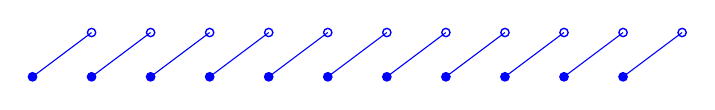
\begin{tikzpicture}[scale=0.75,yscale=0.75]
    \tkzInit[xmin = -5, xmax = 5, ymin = -5, ymax = 5]
    \tkzAxeXY
    \foreach \a in {-5,...,5}{
        \draw[blue] (\a, 0) -- (\a + 1, 1);
        \node [circle, draw, fill, line width = .5pt, color = blue, inner sep = 0pt, minimum size = 3pt] (ca) at (\a, 0) {};
        \node [circle, draw, fill=none, line width = .5pt, color = blue, inner sep = 0pt, minimum size = 3pt] (ca) at (\a + 1, 1) {};
    }
    \end{tikzpicture} $y(x)=\{x\}$
\end{figure}

Now, let's work with these functions to solve some problems.  Most of the problems for this section will focus on the floor function, since it's the most common.
\begin{example}
Compute $\lfloor{\log_2(1000)\rfloor}$.
\end{example}
\begin{solution}
Let $\lfloor{\log_2(1000)\rfloor}=n$.  This means that we can set the inequality $$n\leq\lfloor{\log_2(1000)\rfloor}<n+1,$$ where $n\in\mathbb{Z}$.  Converting the inequality to exponential, we get $$2^n\leq 1000<2^{n+1}.$$  Since $512=2^9\leq 1000<2^{10}=1024$, this means that $n=\lfloor{\log_2(1000)\rfloor}=9$. $\Box$
\end{solution}
\begin{example}
Find all $x$ such that $\left\lfloor{3x+\dfrac{1}{2}}\right\rfloor=7$.
\end{example}
\begin{solution}
Because $\left\lfloor{3x+\dfrac{1}{2}}\right\rfloor=7$, we know that $3x+\dfrac{1}{2}$ is between $7$ and $8$, meaning $$7\leq 3x+\dfrac{1}{2}<8.$$  This is something we know how to solve.  Solving this gives us $$7\leq 3x+\dfrac{1}{2}<8 \implies \dfrac{13}{2}\leq x<\dfrac{15}{2} \implies \dfrac{13}{6}\leq x<\dfrac{5}{2}.$$ $\Box$
\end{solution}
\begin{example}
Find all $x$ such that $2<\lfloor{4x-5}\rfloor\leq 8$.
\end{example}
\begin{solution}
Since $\lfloor{4x-5}\rfloor$ must be an integer, we can change the lower bound to the next integer, $4$.  This makes the inequality $4\leq \lfloor{4x-5}\rfloor\leq 8$.  This means that $4x-5$ is a number between $4$ and $9$, so we can remove the floor notation and write $4\leq 4x-5<9$.  Solving for $x$ gives $$4\leq 4x-5<9 \implies 9\leq 4x<14 \implies \dfrac{9}{4}\leq x<\dfrac{7}{2}.$$ $\Box$
\end{solution}
The final type of problem that the floor function is used for is evaluating the approximate value of large operations without a calculator.  We will try one example of this.
\begin{example}
Evaluate $\left\lfloor{\dfrac{2007^3}{2005 \cdot 2006}-\dfrac{2005^3}{2006\cdot 2007}}\right\rfloor$ without a calculator.
\end{example}
\begin{solution}
We will not multiply this all out; it would take way too long and there's too many places to make mistakes.  Instead, we will use some algebra to simplify it.  If we let $n=2005$, we can write the expression in terms of $n$ and then simplify from there.  \begin{align*}
    \dfrac{2007^3}{2005 \cdot 2006}-\dfrac{2005^3}{2006\cdot 2007}&=\dfrac{(n+2)^3}{n(n+1)}-\dfrac{n^3}{(n+1)(n+2)}=\dfrac{(n+2)^4-n^4}{n(n+1)(n+2)} \\
    &=\dfrac{8n^3+24n^2+32n+16}{n(n+1)(n+2)}=\dfrac{8(n+1)(n^2+2n+2)}{n(n+1)(n+2)} \\
    &=\dfrac{8(n^2+2n+2)}{n(n+2)}=\dfrac{8n(n+2)+16}{n(n+2)} \\
    &=8+\dfrac{16}{n(n+2)} 
\end{align*}
We've made significant process!  Now, what to do with the $\dfrac{16}{n(n+2)}$ term? Well, at $n=2005$, we know that $0<\dfrac{16}{n(n+2)}<1$, meaning that $$\left\lfloor{\dfrac{2007^3}{2005 \cdot 2006}-\dfrac{2005^3}{2006\cdot 2007}}\right\rfloor=8.$$ $\Box$
\end{solution}
Those are the basic problems that you'll experience when it comes to the floor function.  Now, let's look at some harder problems using the same methods.
\section{Problem-Solving with the Floor Function}
\noindent The goal of this section is to over various approaches when it comes to the floor function.  These aren't new techniques, but rather are different ways of looking at harder problems using the same techniques.
\begin{example}
Find all values of $x$ such that $x+\lfloor{x}\rfloor=6.7$.
\end{example}
\begin{solution}
The easiest way to do this is to split the answer into two parts (the integer and the fractional part). We know that the only way to get the $0.7$ part of the answer is from the $x$, meaning $x$ must have $0.7$ in it.  That leaves the integer component of $x$ and $\lfloor{x}\rfloor$.  Since both must be the same, we know that $\lfloor{x}\rfloor=3$.  This means that $x=3.7$.

If you don't understand how that works, note that $x=\lfloor{x}\rfloor+\{x\}$.  This way, we get $2\lfloor{x}\rfloor+\{x\}=6.7$, which makes $x=3.7$ by splitting the equation. $\Box$
\end{solution}
\begin{example}
Find all real numbers $x$ such that $\lfloor{x}\rfloor=5x-14$.
\end{example}
\begin{solution}
Again, for this one, we will use the idea that $x=\lfloor{x}\rfloor+\{x\}$.  This gives us $$\lfloor{x}\rfloor=5\lfloor{x}\rfloor+5\{x\}-14.$$  Solving for $\{x\}$, we get $$\{x\}=\dfrac{14-4\lfloor{x}\rfloor}{5}.$$  Since $0\leq \{x\}<1$, we have $0\leq \dfrac{14-4\lfloor{x}\rfloor}{5}<1$.  Solving this for $x$ gives us $$0\leq 14-4\lfloor{x}\rfloor<5 \implies \dfrac{9}{4}<\lfloor{x}\rfloor\leq \dfrac{7}{2}.$$  The only integer on the interval is $3$, meaning that $\lfloor{x}\rfloor=3$.  Therefore, $\{x\}=\dfrac{14-4\cdot 3}{5}=\dfrac{2}{5}$.  Thus, $x=\lfloor{x}\rfloor+\{x\}=\dfrac{17}{5}=3.4$. $\Box$
\end{solution}
For the final problem in this chapter, we are going to do a summation.  Don't be alarmed; this is not a difficult problem.  We just need to understand what we are adding and find a way to evaluate an equivalent sum that's easier to add.
\begin{example}
Find $\displaystyle \sum_{k=1}^{99}{\left\lfloor{\sqrt{k}}\right\rfloor}$.
\end{example}
\begin{solution}
Let's expand the summation to take a look at what we are adding: $$\sum_{k=1}^{99}{\left\lfloor{\sqrt{k}}\right\rfloor}=\left\lfloor{\sqrt{1}}\right\rfloor+\left\lfloor{\sqrt{2}}\right\rfloor+\left\lfloor{\sqrt{3}}\right\rfloor+\left\lfloor{\sqrt{4}}\right\rfloor+\left\lfloor{\sqrt{5}}\right\rfloor+\cdots+\left\lfloor{\sqrt{99}}\right\rfloor.$$
The first way to do this is brute force.  We know that $\left\lfloor{\sqrt{1}}\right\rfloor=1$, $\left\lfloor{\sqrt{2}}\right\rfloor=\left\lfloor{\sqrt{3}}\right\rfloor=1$.  The next term is then $\left\lfloor{\sqrt{4}}\right\rfloor=\left\lfloor{\sqrt{5}}\right\rfloor=\left\lfloor{\sqrt{6}}\right\rfloor=\left\lfloor{\sqrt{7}}\right\rfloor=\left\lfloor{\sqrt{8}}\right\rfloor=2$, and then $\left\lfloor{\sqrt{9}}\right\rfloor=3$.

There is a clear pattern here.  We first notice that we can solve this by counting the number of values between the perfect squares and then multiply by their floor function (since they're all the same).  This is the simple way to do it.  We are going to follow this method but provide a more mathematical explanation.

Our goal is to find all integers $k$ such that $\left\lfloor{\sqrt{k}}\right\rfloor=m$, where $m$ is a positive integer.  This means that $m\leq \sqrt{k}<m+1$, so $m^2\leq k<(m+1)^2$.  Counting the number of integers in this list, $k$ must be one of $m^2$, $m^2+1$, $m^2+2$, $\ldots$, $(m+1)^2-1$.  There are $((m+1)^2-1)-(m^2)+1=2m+1$ integers in this list.  These integers are then multiplied by $m$.  There are $9$ perfect squares in the range, meaning $m$ ranges from $1$ to $9$.

This means that we can rewrite the given summation as $$S=\sum_{k=1}^{99}{\left\lfloor{\sqrt{k}}\right\rfloor}=\sum_{m=1}^{9}{m(2m+1)}.$$  Evaluating the sum by plugging in each value of $m$, we get $$S=3+10+21+36+55+78+105+136+171=615.$$ $\Box$
\end{solution}
This is all we have to cover.  This chapter was somewhat on the short side; we reviewed one function and introduced another.  Although you won't see the floor function as often in regular mathematics classes, it's a good skill to know how to use and implement.  Courses that focus on competition preparation will go into much greater detail on these functions.
\begin{reviewset}
\item Simplify $\left|x-\sqrt{(x-9)^2}\right|$ for all $x<0$. \vspace{3mm}
\item Show that $\lceil{x}\rceil=-\lfloor{-x}\rfloor$ for all $x\in\mathbb{R}$. \vspace{3mm}
\item Find $f^{-1}(x)$ if $f(x)=x|x|+2$. \vspace{3mm}
\item Find all constants $c$ such that $|cx-1|+|x^2-x-2|=0$ has a solution in $x$. \vspace{3mm}
\item Let $a$ and $b$ be distinct real numbers.  Find $x$ in terms of $a$ and $b$ such that $|x-a|=|x-b|$. \vspace{3mm}
\item Find all ordered pairs $(x.y)$ such that $|x|+|y|=10$ and $xy=24$. \vspace{3mm}
\item Let $a$, $b$, and $c$ be real numbers such that $|a|=|b-2|$, $|b|=|c-2|$ and $|c|=|a-2|$.  Prove that $a+b+c=3$.  \vspace{3mm}
\item Determine whether the following functions are continuous. Then, determine if the function has an inverse; if so, find it. \newline
(a) $f(x)=\begin{cases} 4x & x<5 \\ 5/x & x\geq 5 \end{cases}$. \hspace{30mm}
(b) $g(x)=\begin{cases} 2x & x<2 \\ 2^x & x\geq 2 \end{cases}$. \vspace{3mm}
\item Evaluate $\left\lfloor{\log_2\sqrt{999}}\right\rfloor$ without the use of a calculator.  \vspace{3mm}
\item How many ordered triples of integers $(a,b,c)$ satisfy $|a+b|+c=19$ and $ab+|c|=97$? \vspace{3mm}
\item Find the values of $x$ that satisfy $\left\lfloor{\sqrt{2x-7}}\right\rfloor=9$. \vspace{3mm}
\item Find all integers $x$ such that $\lfloor{x/6}\rfloor=5$. \vspace{3mm}
\item Compute $\left\lfloor{\sqrt{n^2-10n+29}}\right\rfloor$ when $n=20252025$. \vspace{3mm}
\item Find all values of $x$ such that $7x+\lfloor{2x}\rfloor=52$. \vspace{3mm}
\end{reviewset}
\begin{challengeset}
\item Find all real values of $x$ such that $\left\lfloor{\left|-x^2+10x-16\right|}\right\rfloor=1$. \vspace{3mm}
\item Find $\dfrac{\{\sqrt{3}\}^2-2\{\sqrt{2}\}^2}{\{\sqrt{3}\}-2\{\sqrt{2}\}}$ without a calculator. \vspace{3mm}
\item Graph $f(x)=\lfloor{x}\rfloor+\lceil{x}\rceil$ and $g(x)=\lceil{x}\rceil-\lfloor{x}\rfloor$. \vspace{3mm}
\item Find the largest real positive number $\delta$ such that $\left|\sqrt{x}-2\right|<0.1$ if $|x-4|<\delta$. \vspace{3mm}
\item Let $S_n=\lfloor{1}\rfloor+\lfloor{2}\rfloor+\lfloor{3}\rfloor+\cdots+\lfloor{n}\rfloor$ where $n\in\mathbb{Z}$.  Find the largest value of $k<2021$ such that $S_{2021}-S_k$ is a perfect square. \vspace{3mm}
\item What positive, real number $x$ has the property that $x$, $\lfloor{x}\rfloor$, and $x-\lfloor{x}\rfloor$ form a geometric progression?\vspace{3mm}
\item Find the domain of $f(x)=\dfrac{\sqrt{64-x^2}}{\sqrt[4]{16-|2x+5|}}$. \vspace{3mm}
\item Find the smallest real number $x$ such that $\dfrac{x}{\lfloor{x}\rfloor}=\dfrac{2002}{2003}$. \vspace{3mm}
\item Graph $f(x)=\lfloor{2x}\rfloor+\lfloor{4x}\rfloor+\lfloor{6x}\rfloor+\lfloor{8x}\rfloor$. \vspace{3mm}
\item The function $f$ is defined on $\mathbb{Z}$ and satisfies $$f(n)=\begin{cases} n-3 & n\geq 1000 \\ f(f(n+5)) & n<1000\end{cases}.$$  Find $f(84)$. \vspace{3mm}
\item Define $f(n)$ by $$\begin{cases} n/2 & \text{if } n \text{ is even} \\ (n+1023)/2 & \text{ if } n \text{ is odd} \end{cases}.$$  Find the least positive integer such that $f(f(f(f(f(n)))))=n$. (HINT: Experiment with small values of $n$.  Also, use the fact that there are lots of $2$'s.  How could we go about writing $n$ to make this problem easier?) \vspace{3mm}
\end{challengeset}

%%%%%%%%%%%%%%%%%%%%%%%%%%%%%% CHAPTER 11 %%%%%%%%%%%%%%%%%%%%%%%%%%%%%%%%%%%%%%%%%%%%%
\chapter{Systems of Equations}
\begin{introduction}[Contents]
\item Solutions to Systems via Graphing
\item Solutions to Linear Systems via Substitution
\item Solutions to Linear Systems via Elimination
\item Larger Systems of Linear Equations
\item Solutions to Non-Linear Systems
\item Solutions to Non-Linear Systems via Substitution
\end{introduction}
\noindent This chapter is going to discuss systems of equations.  We are going to cover what linear system are and how to solve them.  A natural extension from covering the math of a given linear relationship is to ask what it would mean to have more than one.  This idea is extremely applicable to the real world $-$ many problems needed to be solved have more than one relationship which needs to hold; these “requirements” lend themselves naturally to multiple equations, of which are often linear.  

\begin{remark}
  A linear system of equations is a set of multiple linear equations.  The “solution” can be thought of as asking “for what values do all of these equations in the system hold?”
\end{remark}
\section{Solutions to Systems via Graphing}
Three different methods will be taught to find the solution to a given system.  We’ll start with arguably the easiest to understand: graphing.  Looking for the solution to a system $-$ when all of the (linear) equations hold $-$ is the same as searching for a set of values which lie on the graphs of each equation.

\begin{wrapfigure}{r}{5cm}
    \begin{tikzpicture}[xscale=0.25,yscale=0.25]
         \draw[<->] (-10,0) -- (10,0) node[right] {$x$};
      \draw[<->] (0,-10) -- (0,10) node[above] {$y(x)$};
      \draw[scale=1,domain=-10:10,smooth,variable=\x,blue] plot ({\x},{-\x});
      \draw[scale=1,domain=-6.5:3.5,smooth,variable=\x,red] plot ({\x},{2*\x+3});
      \filldraw (-1,1) circle[radius=7pt] node[left=1mm] {$(-1,1)$};
     \end{tikzpicture} 
\end{wrapfigure}

Let’s look at an example where we have two variables (so we can graph in the Cartesian plane) and two equation:

\begin{example}
Find the solution to $\begin{cases} 2x-y=-3 \\ x+y=0 \end{cases}$ via graphing.
\end{example}
\begin{solution}
Remember, we want to find a value or set of values which lie on both lines; this is essentially asking to find the intersection point of the two lines.

Based on the graph to the right, we can see that $(-1,1)$ is our solution to the system.  Let’s check our answer by plugging these coordinates back into the original equations.  \begin{align*}
    \text{EQN 1:}& \hspace{0.25in} 2(-1)-(1)=-3 \\ \text{EQN 2:}& \hspace{0.25in}  (-1)+(1)=0
\end{align*}$\Box$
\end{solution}
\begin{remark}
  Graphing to solve systems is rarely used as it can be inaccurate if it is done by hand.
\end{remark}
\begin{wrapfigure}{r}{5cm}
    \begin{tikzpicture}[xscale=0.25,yscale=0.25]
         \draw[<->] (-10,0) -- (10,0) node[right] {$x$};
      \draw[<->] (0,-10) -- (0,10) node[above] {$y(x)$};
      \draw[scale=1,domain=-3:1.5,smooth,variable=\x,blue] plot ({\x},{2*\x*\x+3*\x+1});
      \draw[scale=1,domain=-10:-0.1,variable=\y,red] plot({1-1/\y},{\y});
      \draw[scale=1,domain=0.1:10,variable=\y,red] plot({1-1/\y},{\y});
     \end{tikzpicture} 
\end{wrapfigure}

We won't spend too much longer on this topic, but we considered it important to cover the solution to a non-linear system.  Take a look at the example below.

\begin{example}
Solve the system $\begin{cases} 2x^2+3x+1=y \\ 1-\dfrac{1}{y}=x \end{cases}$ via graphing.  You may use a graphing calculator for this problem.
\end{example}
\begin{solution}
Our goal is to find the intersection point(s) between the two graphs shown.  Looking at the graph to the right, we see that there are three intersection points between these plots.  We can find these using a graphing calculator or via algebra.  

To solve this algebraically, use substitution to have an equation in terms of $y$ and solve.  We encourage you to try this on your own, but we will not show this method.  

Most students will be solving with a TI-84 Calculator.  Using the graphing menu, we plot both functions (solve the bottom function for $y$ first).  Then, using the intersect feature, we find the three intersection points to be $$(-1.281,0.438) \hspace{0.15in} (0,1) \hspace{0.15in} (0.781, 4.562).$$ $\Box$
\end{solution}
With that done, let's move on to a more accurate solution: substitution.
\section{Solutions to Linear Systems via Substitution}
Substitution, a more algebraic method that works very well in linear equations, involves taking on of the equations and isolating a variable; this isolated variable can then be substituted into the other equation(s) where standard algebra can then solve the rest.  

Let's run through the different cases of this so you're prepared for everything.
\begin{example}
Solve the system of equations $\begin{cases} x+y=4 \\ 3x-2y=2 \end{cases}$ via substitution.
\end{example}
\begin{solution}
\noindent The first thing we need to do is isolate a variable from one of the equations.  In this case, the first equation is easier to do this.  We choose to isolate $y$; however, this is your choice.  We get that $y=4-x$.

Now, we plug this into the second equation.  This gives $$3x-2(4-x)=2 \implies 3x-8+2x=2 \implies 5x=10 \implies x=2.$$  Then, plug this back into one of the equations to solve for $y$.  
$$(2)+y=4 \implies y=2.$$  This means that the solution, written as an ordered pair, is $(2,2)$.  This can be verified via graphing if you choose; we won't show it.  $\Box$
\end{solution}
In this case, the solution was an ordered pair.  But we obviously know that there are cases where this may not be true.  Let's look at another case.
\begin{example}
Solve the system of equations $\begin{cases} 2x-y=4 \\ 4x-2y=3 \end{cases}$ via substitution.
\end{example}
\begin{solution}
It seems easiest in this case to solve the first equation for $y$.  Doing this makes $$2x-y=4 \implies 2x=y+4 \implies 2x-4=y.$$  Then, plug this into the second equation.  $$4x-2(2x-4)=3 \implies 4x-4x+8=3 \implies 8=3.$$  We know this not to be true.  This must mean that there is no solution.  $\Box$
\end{solution}

\begin{remark}
  In upper-level math courses, it is most common to label problems with no solutions as DNE, which stands for (the solution) Does Not Exist.
\end{remark}

One way we could have quickly verified this solution is simplifying the second equation.  Dividing by $2$, we would've gotten $2x-y=\dfrac{3}{2}$.  We know this can't be equal to the first equation; thus, it has no solutions.

Let's look at one final case that's not so obvious.
\begin{example}
Solve the system of equations $\begin{cases} -x-y=2 \\ 2x+2y=4 \end{cases}$ via substitution.
\end{example}
\begin{solution}
It might be easier in this case to use the second equation to avoid the use of negative signs.  Solving for $x$ in this case, we get $$2x=-4-2y \implies x=-2-y.$$  Plugging this into the first equation gives $$-(-2-y)-y=2 \implies 2+y-y=2 \implies 2=2.$$  This is true no matter what, which means that the system has infinite solutions.  $\Box$
\end{solution}
We also might note that in this case, both equations were technically the same.  Multiplying the top equation by $-1$ and the bottom by $\dfrac{1}{2}$ yields $x+y=-2$ for both.  This means that they represent the same line; thus, there are infinite solutions.

Every point on this line will produce a solution to the system, for this reason there are infinite solutions to this specific system.  Therefore, the solution to the system can be written as follows: $$y=-x-2, \hspace{0.25in} x\in\mathbb{R}.$$  Writing it like this allows us to classify the types of solutions, since obviously not all pairs work.

\begin{remark}
This is how all infinite solutions should be written.  It lets the grader know that there is a classification of solution.  Write it in terms of a dependent variable and define the domain of the independent variable.
\end{remark}

These are the necessary sections that we need to cover.  Now let's discuss a better method for solving linear systems if it's not easy to isolate a variable: elimination.
\section{Solutions to Linear Systems via Elimination}
\noindent The goal of this section is to provide a method in which you don't need an isolated variable.  When coefficients start growing, you'll be left with messy fractions when you use substitution; however, using elimination will help to fix this.

\textit{Elimination} is the process of finding the least common multiple between the same variable in both equations and transforming them such that they then have the same coefficient.  Then, using basic inspection, we solve for the other variable.

This is a little tough to explain without looking at some examples.  Let's try a few.
\begin{example}
Solve the system $\begin{cases} 6x-3y=3 \\ 2x+y=-5 \end{cases}$ using elimination.
\end{example}
\begin{solution}
Let's consider each example using some intuition.  The first equation has a common factor of $3$, so let's remove it.  This gives $2x-y=1$ for the new first equation.  We see that both $x$ and $y$ have the same magnitude in these equations, yet $y$ has an opposite sign.  In this case, we will add both equations together to eliminate $y$.  This leaves $4x=-4$, meaning $x=-1$.

To solve for the other variable, plug it into one of the equations.  We'll use the second.  This means that $$2(-1)+y=-5 \implies -2+y=-5 \implies y=-3.$$ $\Box$
\end{solution}

\begin{remark}
We could've eliminated $x$ instead of $y$ and we would've received the same answer.  Instead of adding both equations to eliminate $y$, we would've subtracted the equations to eliminate $x$.  Note that this is not always true; this happened out of coincidence.  
\end{remark}

Let's look at a similar example that requires one extra step.
\begin{example}
Solve the system $\begin{cases} -2x+3y=5 \\ 5x+4y=8\end{cases}$ using elimination.
\end{example}
\begin{solution}
We see that in this case, there is no obvious first step.  We know that we must eliminate one of the variables by determining the least common multiple; however, there isn't an easy choice.  In this case, and in all other cases, we will choose the variable with opposite signs for coefficients.  Thus, we choose $x$ as the variable to eliminate.  

The least common multiple between $2$ and $5$ is $2\cdot 5=10$.  To get there, we multiply the top equation by $5$ and the bottom equation by $2$.  This makes the new system $$\begin{cases} -2x+3y=5 \\ 5x+4y=8\end{cases}\implies \begin{cases} -10x+15y=25 \\ 10x+8y=16 \end{cases}.$$  Since the $x$-coefficients are the same, we add the equations.  This yields the resultant equation $23y=41$, meaning $y=\dfrac{41}{23}.$  Plugging this back into one of the equations to solve for $x$ (we will use the second equation), we get $$5x+4\left(\dfrac{41}{23}\right)=8 \implies 5x+\dfrac{164}{23}=\dfrac{184}{23} \implies 5x=\dfrac{20}{23}\implies x=\dfrac{4}{23}.$$  This makes the solution of the system $\left(\dfrac{4}{23},\dfrac{41}{23}\right)$.  $\Box$
\end{solution}

\begin{remark}
If both variables have coefficients of the same sign, then choose the one with the smaller least common multiple.  If this isn't terribly obvious, choose the ones with the smaller coefficients.
\end{remark}

Now, let's discuss the process of solving larger systems.
\section{Larger Systems of Linear Equations}
\noindent This section is going to look at systems with more equations and more coefficients.  In this section, most problems will have a variable with a subscript (ex: $x_1$ and $x_2$) to represent the independent variables.  It often becomes confusing to introduce too many letters of the alphabet, so we use this system instead.

Often, problems like this can be tedious to solve for every variable and can be sometimes annoying to write down all the solutions.  To avoid this, some problem writers will choose to ask you to give your answer as an expression in terms of these variables.  However, there are times when we can find this value without ever solving for one or more of the variables.  We will discuss how this happens later in this section.

Now, we will try to solve a $3\times 3$ system of equations (this means there are $3$ variables and $3$ equations).
\begin{example}
Solve the system of equations $\begin{cases} -2x+y+z=4 \\ -x+y-z=3 \\ x-y=-1 \end{cases}$ using a method of your choice.
\end{example}
\begin{solution}
We quickly note that graphing seems like a bad idea, as we would have to graph in three-dimensional space.  Since we don't know how to do that yet, and you won't learn until Calculus 3, we aren't going to worry about it.

Substitution doesn't seem like a bad idea in this case, especially with the third equation.  If we solve for $x$ in terms of $y$ (or vice versa), we can plug this into the other equations and reduce it down to a $2\times 2$ system.  From the third equation, we have $x=y-1$.  Plugging this into the other equations we have $$\begin{cases} -2(y-1)+y+z=4 \\ -(y-1)+y-z=3 \end{cases} \implies \begin{cases} -2y+2+y+z=4 \\ -y+1+y-z=3 \end{cases} \implies \begin{cases} -y+z=2 \\ -z=2 \end{cases}.$$  We quickly find that $z=-2$ and start plugging this back into the other equations.  Plugging this into $-y+z=2$, we get $y=-4$.  Plugging $y$ into the original substitution, we get $x=-4-1=-5$.

We write the solution as an ordered triple, so the solution is $(-5,-4,-2)$.  $\Box$
\end{solution}
Let's try another example with a $3\times 3$ system.
\begin{example}
Find the solutions $x_1$, $x_2$, and $x_3$ that satisfy $\begin{cases} x_1+x_2+x_3=6 \\ x_1+2x_2+3x_3=14 \\ 2x_1+5x_2+8x_3=36 \end{cases}$.
\end{example}
\begin{solution}
Again, graphing isn't a plausible solution.  Substitution could be done but elimination is a better option.  In problems like this, we want to eliminate one variable (the same variable) from two of the three equations.  In this case, we will eliminate $x_1$.  To do this, we subtract equation $1$ from equation $2$, and then subtract twice equation $1$ from equation $3$.  Mathematically, this looks like \begin{align*}
    \text{EQN } 1 - \text{EQN } 2&: (x_1+x_2+x_3)-(x_1+2x_2+3x_3)=(6)-(14) \implies -x_2-2x_3=-8\\
    2\text{EQN } 1 - \text{EQN } 3&: 2(x_1+x_2+x_3)-(2x_1+5x_2+8x_3)=2(6)-36 \\
    &\implies -3x_2-6x_3=-24 \implies -x_2-2x_3=-8.
\end{align*}
We see that we got the same equation twice!  That means that we have a dependent system where there are infinite solutions.  Like the example in \hyperlink{section.11.2}{Section 11.2}, we must find a solution in terms of other variables.

We can quickly see that $x_2=8-2x_3$.  Let's solve for $x_1$ in terms of $x_3$ using the first equation.  This gives $$x_1+(8-2x_3)+x_3=6 \implies x_1-x_3=-2 \implies x_1=x_3-2.$$  So, in this case, we write the solution as $(x_3-2,8-2x_3,x_3), \hspace{0.10in} x_3\in\mathbb{R}$.  $\Box$
\end{solution}
This doesn't always happen.  There is a case, however, where it is obvious that there will be a parameter.  This is when there are less equations than the number of variables.  There is no way to solve for more variables than there are equations, meaning we must write the answers in terms of other variables.  This will be showcased in the review problems.

\begin{remark}
You may be wondering: what happens if there are more equations than variables?  This is a great question that leads to a similar answer.  There are a few possibilities here: all the systems could work out and leave one system.  Or, one of the equations could simply be repetitive (whether it be a multiple of one of the equations, the sum of two other equations, etc.), which leaves it no value and can be ignored.  Otherwise, the equations won't work together (this is the most common) and leads to no solutions.
\end{remark}

Often, for systems of equations with more than three variables, elimination is the best method.  This is usually since there isn't an equation only in terms of two variables.  To solve these, try to reduce the system to $3\times 3$ with the least number of operations, and solve from there.  The goal is to always reduce one variable at a time until you reach the $2\times 2$, which is easily solvable.

Now, let's discuss the final type of larger system that there might be: when the question asks for an answer in terms of other variables.  This is somewhat common if there are less equations than variables, but is also seen when there are as many equations as variables.
\begin{example}
Find $x-y+z$ if $3x-y+5z=44$ and $x+2z=12$.
\end{example}
\begin{solution}
We see that we have more variables than equations, so we either have to find each variable in terms of another or we can find $x-y+z$ head-on.  Let's work on getting there one variable at a time, starting with $x$.  Subtracting twice equation $2$ from equation $1$, we get $$(3x-y+5z)-2(x+2z)=(44)-2(12)=x-y+z=20.$$  Turns out, we made it without any extra work!  So the answer is $20$.  $\Box$
\end{solution}
These are the types of larger systems of equations.  Note that there wasn't much new in this section - we simply used what we knew and applied it in a larger scenario.  Now, let's move on to non-linear systems, where we will have to slightly modify our methods to solve them.
\section{Solutions to Non-Linear Systems}
This section is going to involve a lot of substitution.  Substitution will serve as the best method for nearly every problem in this section and the next section.  Most problems here will be $2\times 2$ systems.  Our goal is to combine the equations such that we have an equation we know how to solve - a high percentage of them will be quadratics (or hidden quadratics).  

The best way to learn to solve these is by example.  Let's get started.
\begin{example}
Solve the system of equations $\begin{cases} x-y=3 \\ \dfrac{1}{x}+\dfrac{1}{y}=\dfrac{1}{2} \end{cases}$ using substitution.
\end{example}
\begin{solution}
Substitution will be much easier with the top equation.  We see that $x=y+3$, so we plug that into the bottom equation.  Doing this and simplifying, we get $$\dfrac{1}{y+3}+\dfrac{1}{y}=\dfrac{1}{2} \implies \dfrac{2y+3}{y(y+3)}=\dfrac{1}{2}.$$  Cross-multiplying gives us the equation $$2(2y+3)=y^2+3y \implies 4y+6=y^2+3y \implies y^2-y-6=0.$$  This is a simple quadratic we can factor to solve.  This gives $(y-3)(y+2)=0 \implies \begin{matrix} y_1=-2 \\ y_2=3 \end{matrix}.$

Before we continue, we need to make sure that both of these solutions are valid.  The only way they couldn't be valid is if $y=0$, which isn't true; thus, they are both valid.

Now, we plug them back into the first equation (the easier equation) to solve for $x$.  This gives $\begin{matrix} x_1+2=3 \implies x_1=1 \\ x_2-3=3 \implies x_2=6 \end{matrix}$.  Thus, our two solutions are $\left(1,-2\right)$ and $\left(6,3\right)$.  $\Box$
\end{solution}

Let's look at an example where elimination may be the better choice.
\begin{example}
Find all solutions $(x,y)$ such that $\begin{cases} x^2+xy=126 \\ x^2-xy=36 \end{cases}$ holds true.
\end{example}
\begin{solution}
In this case, we want to remove the $xy$ term, and we can do this very easy via adding the two equations.  Doing this gives us $2x^2=162$, meaning that $x^2=81$.  We get two solutions: $x_1=-9$ and $x_2=9$.  

Quickly checking that there are no domain restrictions, we then move on to find $y$.  Plugging in the values of $x$ into the top equation, we get $\begin{matrix} 81-9y=126 \implies y=-5 \\ 81+9y=126 \implies y=5 \end{matrix}$.  This means that our two solutions are $(-9,-5)$ and $(9,5)$.  $\Box$
\end{solution}
\begin{note}
Something you should always do after every problem is check the solutions to make sure that they're valid.  We haven't been doing this throughout the problems to maintain the brevity of the solutions; however, it is important you practice this in the review problems.
\end{note}
There are quite a few types of these and they all encompass the same methodology.  Thus, we aren't going to show any more examples.  When you encounter problems like this, we urge you to follow one of two ideas: (1) use elimination to get rid of the non-linear terms \textit{or} convert it to something you can eliminate (such as a perfect square trinomial), or (2) use substitution to get rid of a variable and solve the for the other.

Now, let's expand on the idea of substitution to simplify the system.
\section{Solutions Non-Linear Systems via Substitution}
\noindent Throughout this chapter, we've covered the most basic use of substitution.  The goal of this substitution was to simplify the equation into a single-variable linear equation.  In this case, however, we are going to typically make two substitutions to make a system of equations that's easier to understand.  Let's look at the easiest type.
\begin{example}
Find all pairs $(x,y)$ such that $\begin{cases} x+y+\sqrt{x+y}=30 \\ x-y+\sqrt{x-y}=12 \end{cases}$ is satisfied.
\end{example}
\begin{solution}
In this case, there is no simple way to isolate $x$ or $y$, and even if we add them, the square root terms will still be there.  To fix this, we need a way to get rid of the square root terms.  So, to fix this, we introduce two new variables.  We assign $u=\sqrt{x+y}$ and $v=\sqrt{x-y}$.

Doing this allows us to remove the square roots from both equations and be left with two quadratic equations.  We now have the system $\begin{cases} u^2+u=30 \\ v^2+v=12 \end{cases}$.  Since the equations are independent of one another (they don't share variables), we solve each individually.

The solutions to the first equation are $u=-6$ and $u=5$.  The solutions to the second equation are $v=-4$ and $v=3$.  Remember that $u$ and $v$ both represent square root quantities, so neither can be negative.  Thus, we are left with $u=5$ and $v=3$.  Substituting the values of $u$ and $v$, we get $\begin{cases} \sqrt{x+y}=5 \\ \sqrt{x-y}=3 \end{cases}$.  We can easily square both sides to get $\begin{cases} x+y=25 \\ x-y=9 \end{cases}$.  Solving both equations using basic elimination gives $(x,y)=(17,8)$.  $\Box$
\end{solution}
Let's try a different style of problem that still encompasses the same principle as the previous problem.
\begin{example}
Solve $\sqrt{3x^2-4x+34}+\sqrt{3x^2-4x-11}=9$ for $x$.
\end{example}
\begin{solution}
The first thing you might be wondering is why this is in the Systems of Equations chapter.  It's not a system!  What we'll find out is that making a substitution like this will create a small system that we have to solve.  It won't be tough but it's part of the process.

Let's let $a=\sqrt{3x^2-4x+34}$ and $b=\sqrt{3x^2-4x-11}$.  This means that $a+b=9$.  Let's take advantage of the fact that $a$ and $b$ only differ by a constant.  Squaring both terms and subtracting, we get $$a^2-b^2=(3x^2-4x+34)-(3x^2-4x-11)=45.$$  So, we now have the system $\begin{cases} a+b=9 \\ a^2-b^2=45 \end{cases}$.  Factoring the bottom and substituting the top equation, we get $(9)(a-b)=45 \implies a-b=5$.  This reduces the system to $\begin{cases} a+b=9 \\ a-b=5 \end{cases}$.  We can easily solve this to get $(a,b)=(7,2)$.  It doesn't matter which we use, so we'll use the second.  This gives $$b=\sqrt{3x^2-4x-11}=2 \implies 3x^2-4x-11=4 \implies 3x^2-4x-15=0 \implies \begin{matrix} x_1=-5/3 \\ x_2=3 \end{matrix}.$$$\Box$
\end{solution}
Let's try one that uses elimination to manipulate the equations into something solvable.
\begin{example}
Find all solutions to the system of equations $\begin{cases} 2x^2+3y^2-4xy=3 \\ 2x^2-y^2=7 \end{cases}$.
\end{example}
\begin{solution}
We are going to do a style of elimination that eliminates the constants rather than the variables.  Thus, in this case, we are going to subtract three times the bottom equation from seven times the top equation.  This gives $$7(2x^2+3y^2-4xy)-3(2x^2-y^2)=7(3)-3(7) \implies 8x^2+24y^2-28xy=0.$$  Dividing by four on both sides gives $2x^2-7xy+6y^2=0.$  This is something that we can factor.  This factors to $(2x-3y)(x-2y)=0$.  This means that $x=\dfrac{3}{2}y$ or $x=2y$.  Plugging $x=2y$ into the bottom equation gives the solutions $(x,y)=(2,1)$ and $(x,y)=(-2,-1)$.  Letting $x=\dfrac{3}{2}y$ gives $(x,y)=\left(\dfrac{3}{2}\sqrt{2},\sqrt{2}\right)$ and $(x,y)=\left(-\dfrac{3}{2}\sqrt{2},-\sqrt{2}\right)$.  $\Box$
\end{solution}

\begin{remark}
There are other solutions to this problem, but we felt that this was the most simple to understand.  Another solution involves removing the $2x^2$ term from both equations as it's the term they have in common.
\end{remark}

If you don't understand how we factored the multi-variable function, consider making another substitution.  If you divide both sides by $y^2$ and let $z=\dfrac{x}{y}$, it will reduce to a uni-variate quadratic that you can solve using any method from \hyperlink{chapter.5}{Chapter 5}.

There isn't much more to cover in this section.  When you are given a non-linear system, consider whether it may be easier to substitute to simplify.  Other times, you must substitute; otherwise, there won't be a way to isolate one of the other variables or eliminate it.  Consider the use of eliminating constants, as sometimes it's the easiest way to solve.  

You now have many tools in your repertoire to solve different types of systems.  As you traverse through these practice problems, try and think of the easiest method of solving these rather than the first that comes to mind, as there is almost always an easier way.
\begin{reviewset}
\item For each system, solve using the indicated method.  \newline 
(a) $\begin{cases} 2x-5y=-2 \\ -3x+7y=4\end{cases}$ [elimination] \hspace{\stretch{1}}
(b) $\begin{cases} 5x-y=-1 \\ -9x+2y=-2\end{cases}$ [substitution] \newline 
(c) $\begin{cases} -3x+2y=2 \\ -5x+3y=0\end{cases}$ [elimination]\hspace{19mm}
(d) $\begin{cases} 4x+2y=-6 \\ -3x+3y=18\end{cases}$ [graphing]\newline 
(e) $\begin{cases} 6x-3y=9 \\ 4x+2y=18\end{cases}$ [substitution]
\item For each part, determine whether the system of equations has $0$, $1$, or infinite solutions without any manipulation.  \newline 
(a) $\begin{cases} 2x-3y=6 \\ -6x+9y=-18 \end{cases}$ \hspace{50mm} (b) $\begin{cases} 2x-8y=4 \\ -x+4y=-5 \end{cases}$ \newline
\item Solve the following systems using a method of your choice.  \newline 
(a) $\begin{cases} 2x-7y+2z=3 \\ x+4z=1 \\ x-6y-z=2\end{cases}$ \hspace{5mm} (b) $\begin{cases} x+y-2z=-2 \\ -y+3z=1 \\ 4x+y+2z=-4\end{cases}$ \hspace{5mm} (c) $\begin{cases} -5x+y+3z=2 \\ 3x+3y=-3 \\ 2x+4y+z=-3\end{cases}$ \newline
\item Find all pairs $(x,y)$ such that $\begin{cases} xy=1 \\ y=x+1\end{cases}$ holds true.
\end{reviewset}
\begin{challengeset}
\item Solve the system $\begin{cases} 4x+y+z=1 \\ 2x-y+z=3 \end{cases}$ using a method of your choice.
\item Determine the geometric shape produced by $ax+by+cz=d$ where $a,b,c,d\in\mathbb{R}$.  (HINT: the intersection between two of these objects must be a line.)
\item For what values of $k$ does the system of equations $\begin{cases} kx+y+z=k \\ x+ky+z=k \\ x+y+kz=k \end{cases}$ have no solution, infinite solutions, and exactly one solution?
\item Solve the system $\begin{cases} -2x+3y-z=-2 \\ 4x-6y+2z=4 \\ -4x+6y-2z=-4\end{cases}$ using a method of your choice.
\item Find all solutions to the linear piece-wise functions $f(x)=\begin{cases} 2x+2 & x<2 \\ \dfrac{x}{2}+4 & x\geq 2 \end{cases}$ and $g(x)=\begin{cases} 3x-6 & x\geq 0 \\ -6 & x<0\end{cases}$.  (HINT: Graphing may be a good option this time.)
\item Find a set of functions $f(x,y)$, $g(x,y)$, and $h(x,y)$ and constants $k_1$, $k_2$, and $k_3$ such that the solution to the system $\begin{cases} f(x,y)=k_1 \\ g(x,y)=k_2 \\ h(x,y)=k_3 \end{cases}$ has its only solution at $(-1,2)$.
\item Solve the system $\begin{cases} 3y+z-8w=1 \\ -2x+2y-w=-1 \\ x+4y-z+3w=2 \\ 3x+5y-z+2z=-1 \end{cases}$ using a method of your choice.
\item Show that for any system $\begin{cases} f(x)=ax+b \\ f^{-1}(x) \end{cases}$ where $a,b\in\mathbb{R}$, the solution to the system either has no solution or it must lie on $y(x)=x$.
\item Find the area of the region of points that satisfy the system $\begin{cases} y>x \\ x>-x \\ y<x+8 \\ y<-x+8 \end{cases}$.
\item Find all ordered pairs of real numbers $(x,y)$ that satisfy $\begin{cases} x^2+xy=35 \\ y^2+xy=14 \\ x-y=3 \end{cases}$.
\item Find all ordered pairs of real numbers $(x,y)$ that satisfy $\begin{cases} x^3-4y^3=4 \\ 3y^3-x^2y+xy^2=1 \end{cases}$.
\end{challengeset}
%%%%%%%%%%%%%%%%%%%%%%%%%%%%%% CHAPTER 12 %%%%%%%%%%%%%%%%%%%%%%%%%%%%%%%%%%%%%%%%%%%%%
\chapter{Trigonometry}
\begin{introduction}[Contents]
\item The Trigonometric Functions
\item The Unit Circle
\item Solving Trigonometric Equations
\item Graphing Trigonometric Functions
\item Author's Note on Sinusoidal Curves
\end{introduction}
\noindent Well, here we are, trigonometry $-$ what for many Americans is the summit of their mathematical adventure. To keep things relatively simple, we will only be providing an introduction into the field, as the full extent of it will be covered later on during your time in Pre-calculus. Technically, trigonometry is the study of triangles, coming from the roots "tri" for $3$ (sides/angles) and “metry” meaning to measure. In practice, however, trigonometry more often involves the study of certain \textit{trigonometric functions} which enable greater understanding of both triangles and a wide variety of other applications. As you will soon find out, to understand and intuit in place of memorize, trigonometry will often require of you a certain flexibility $-$ to be able to quickly switch between algebraic and geometric perspectives.  
\section{The Trigonometric Functions}
\noindent We’ll start with the very basics. First, since this chapter is about trigonometry, let’s look at some simple cases of triangles. Let’s say we have a right triangle and we know one of the (non-right) angles. For the sake of simplicity, let’s also assume we know the hypotenuse has a length of one. Below are some cases of the above situation:
\begin{figure}[!h]
    \centering
    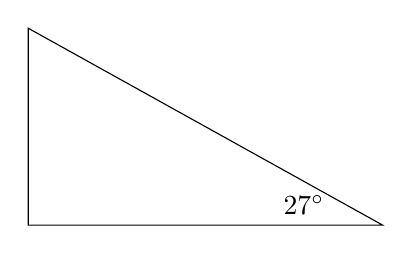
\begin{tikzpicture}[xscale=0.5,yscale=0.5]
        \draw (0,0) -- (9,0) -- (0,5) -- cycle;
        \draw (7,0.5) node {$27^{\circ}$};
    \end{tikzpicture}
    \hspace{0.5cm}
    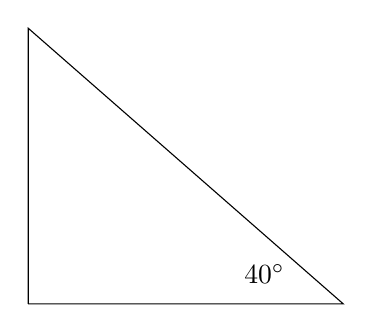
\begin{tikzpicture}[xscale=0.5,yscale=0.5]
        \draw (0,0) -- (0,7) -- (8,0) -- (0,0);
        \draw (6,0.75) node {$40^{\circ}$};
    \end{tikzpicture}
    \hspace{0.5cm}
    \begin{tikzpicture}[xscale=0.5,yscale=0.5]
        \draw (0,0) -- (90:7cm) -- (0:7cm) -- (0,0);
        \draw (5,0.6) node {$45^{\circ}$};
    \end{tikzpicture}
\end{figure}
In these examples, it would be incredibly difficult (if not near impossible) to calculate the length of the other two sides of the triangle. So, in an attempt to make some progress, let’s create some functions $f(\theta)$ and $g(\theta)$ to help us with these cases. $f(\theta)$ will take the known angle $\theta$ as an input to the function and output the length of the side of the triangle \textit{opposite} the angle $\theta$; likewise, $g(\theta)$ will take the known angle $\theta$ as an input and output the length of the side of the triangle \textit{adjacent} the angle $\theta$.

We can observe the general case for this situation below with the known angle $\theta$ and lengths $1$, $f(\theta)$,and $g(\theta)$: \newpage
\begin{figure}
    \centering
    \hspace{\stretch{1}}
    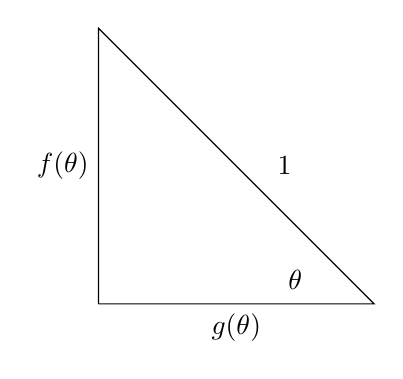
\begin{tikzpicture}[xscale=0.5,yscale=0.5]
        \draw (0,0) -- (90:7cm) node[midway,left] {$f(\theta)$} -- (0:7cm) node[midway,right=0.4cm] {$1$} -- (0,0) node[midway,below] {$g(\theta)$};
        \draw (5,0.6) node {$\theta$};
    \end{tikzpicture}
    \hspace{\stretch{1}}
    \begin{tikzpicture}[xscale=0.5,yscale=0.5]
        \draw (0,0) -- (90:7cm) node[midway,left] {$g(\theta)$} -- (0:7cm) node[midway,right=0.4cm] {$1$} -- (0,0) node[midway,below] {$f(\theta)$};
        \draw (0.65,5.2) node {$\theta$};
    \end{tikzpicture}
    \hspace{\stretch{1}}
\end{figure}
Now it just so happens that these functions are useful enough to where mathematicians have given these two functions special names. $f(\theta)$, the length of the side opposite the angle, is denoted by $\sin(\theta)$; $g(\theta)$, the length of the side adjacent the angle, is denoted by $\cos(\theta)$.
\begin{note}
From here on, $\sin(\theta)$ and $\cos(\theta)$ will be used in place of $f(\theta)$ and $g(\theta)$.  All trigonometric functions will take $\theta$ to be in \textit{radians} instead of \textit{degrees}.
\end{note}
Now that we have all the setup in place, let’s try and calculate some simple cases of $\sin(\theta)$ and $\cos(\theta)$. While you may not be expected to derive some of these without having seen the proof beforehand, it is recommended that you understand them regardless.
\begin{example}
Using principles of geometry, calculate $\sin(0)$ and $\cos(0)$.
\end{example}
\begin{solution}
Consider the left triangle above.  As $\theta$ approaches $0$, we see that $f(0)=\sin(0)$ approaches $0$. Using the Pythagorean Theorem (or similar logic to $\sin(\theta)$ we see that $g(0)=\cos(0)$ approaches $1$. $\Box$
\end{solution}
Here are the figures for the next two problems.  Due to spacing limitations, we were forced to put them above.
\begin{figure}[!h]
    \centering
    \hspace{\stretch{1}}
    \begin{tikzpicture}[xscale=0.5,yscale=0.5]
        \draw (0,0) -- (90:7cm) node[midway,left] {$A$} -- (0:7cm) node[midway,right=0.4cm] {$1$} -- (0,0) node[midway,below] {$B$};
        \draw (0.65,5.2) node {$\theta$};
        \draw (5,0.6) node {$\phi$};
    \end{tikzpicture}
    \hspace{\stretch{1}}
    \begin{tikzpicture}[xscale=0.5,yscale=0.5]
        \draw (0,0) -- (90:5cm) node[midway,left] {$C$} -- (0:9cm) node[midway,right=0.4cm] {$1$} -- (0,0) node[midway,below] {$D$};
        \draw (0.55,3.85) node {$\phi$};
        \draw (7.3,0.6) node {$\theta$};
    \end{tikzpicture}
    \hspace{\stretch{1}}
\end{figure}


\begin{example}
Using principles of geometry, calculate $\sin\left(\dfrac{\pi}{4}\right)$ and $\cos\left(\dfrac{\pi}{4}\right)$.
\end{example}
\begin{solution}
Consider the triangle to the right. We know that the sum of the angles in a triangle must add up to $180^{\circ}$ (or $\pi$), so we know that $\theta=\phi=\dfrac{\pi}{4}$.  This also tells us that $A=B$ (from one of those theorems from Geometry $-$ it says that side lengths are proportional to their angle measure).

Using the Pythagorean Theorem, we can say the following: $$A^2+B^2=1 \implies A^2+A^2=1 \implies A^2=\dfrac{1}{2} \implies A=\dfrac{\sqrt{2}}{2}.$$ This means that we can conclude that $$\sin\left(\dfrac{\pi}{4}\right)=\cos\left(\dfrac{\pi}{4}\right)=\dfrac{\sqrt{2}}{2}.$$ $\Box$
\end{solution}
\begin{remark}
Note that in the example above we didn't accept the negative solution for $A$.  We can't have negative lengths.
\end{remark}
\begin{example}
Using principles of geometry, calculate $\sin\left(\dfrac{\pi}{6}\right)$ and $\cos\left(\dfrac{\pi}{6}\right)$.
\end{example}
\begin{solution}
Based on the diagram to the right, let's set $\phi$ to equal $\frac{\pi}{6}$. Then, we know $\sin\left(\dfrac{\pi}{6}\right)=D$ and $\cos\left(\dfrac{\pi}{6}\right)=C$.

Since all angles in the triangle must add to $\pi$, we calculate $\theta$ to be $\theta=\dfrac{\pi}{2}-\dfrac{\pi}{6}=\dfrac{\pi}{3}.$

Here’s where the clever trick gets involved, notice how $2\phi=\theta$. This fact allows us to leverage some symmetry. The “trick” for this problem is to add a second triangle to the diagram as shown below.
\begin{figure}[!h]
    \centering
    \begin{tikzpicture}[xscale=0.35,yscale=0.35]
        \draw (-9,0) -- (0,0) -- (0,5) -- cycle;
        \draw (0,0) -- (9,0) -- (0,5) -- cycle;
        \draw (-7.25,0.5) node {$\theta$};
        \draw (7.25,0.5) node {$\theta$};
        \draw (-0.5,4.25) node {$\phi$};
        \draw (0.5,4.25) node {$\phi$};
        \draw (0,-0.5) node {$2D$};
        \draw (5,3) node {$1$};
        \draw (-5,3) node {$1$};
    \end{tikzpicture}
    \hspace{\stretch{1}} $\to$ \hspace{\stretch{1}}
    \begin{tikzpicture}[xscale=0.35,yscale=0.35]
        \draw (-9,0) -- (9,0) -- (0,5) -- cycle;
        \draw (0,4.25) node {$\theta$};
        \draw (-7.25,0.5) node {$\theta$};
        \draw (7.25,0.5) node {$\theta$};
        \draw (0,-0.5) node {$2D$};
        \draw (5,3) node {$1$};
        \draw (-5,3) node {$1$};
    \end{tikzpicture}
\end{figure}

By adding on a second triangle we can form one larger triangle with equal angles, an equilateral, and therefore we know all of the side lengths must be equal. This means that $2D=1$, or $D=\dfrac{1}{2}$.

Since we know two out of the three side lengths of the original triangle, we can use the Pythagorean Theorem again. $$C^2+\left(\dfrac{1}{2}\right)^2=1 \implies C^2=\dfrac{3}{4} \implies C=\dfrac{\sqrt{3}}{2}.$$ We can use the definitions for $C$ and $D$ established above to say that $\sin\left(\dfrac{\pi}{6}\right)=\dfrac{1}{2}$ and $\cos\left(\dfrac{\pi}{6}\right)=\dfrac{\sqrt{3}}{2}$. $\Box$
\end{solution}
What if we have a right triangle with a hypotenuse not equal to $1$ and we want to know the lengths of the other sides? Well, we can use a simple property regarding similar triangles.

\begin{figure}
    \centering
    \hspace{\stretch{1}}
    \begin{tikzpicture}[xscale=0.5,yscale=0.5]
        \draw (0,0) -- (90:7cm) -- (0:7cm) -- (0,0);
        \draw (4,0) -- (4,3);
        \draw (5.2,0.6) node {$\theta$};
        \draw[|<->|] (4,-0.75) -- node[fill=white,sloped] {$\cos(\theta)$} (7,-0.75);
        \draw[|<->|] (0,-1.25) -- node[fill=white,sloped] {$c$} (7,-1.25);
        \draw[|<->|] (0.5,8) -- node[fill=white,sloped] {$a$} (8,1);
        \draw[|<->|] (4.5,3.5) -- node[fill=white,sloped] {$1$} (7.5,0.5);
        \draw[|<->|] (-0.75,0) -- node[fill=white] {$b$} (-0.75,7);
        \draw[|<->|] (2.5,0) -- node[fill=white] {$\sin(\theta)$} (2.5,3);
    \end{tikzpicture} \hspace{\stretch{1}} $\to$ \hspace{\stretch{1}}
    \begin{tikzpicture}[xscale=0.5,yscale=0.5]
        \draw (0,0) -- (90:7cm) -- (0:7cm) -- (0,0);
        \draw (5.2,0.6) node {$\theta$};
        \draw[|<->|] (0,-0.75) -- node[fill=white,sloped] {$a\cos(\theta)$} (7,-0.75);
        \draw[|<->|] (0.5,7.5) -- node[fill=white,sloped] {$a$} (7.5,0.5);
        \draw[|<->|] (-0.75,0) -- node[fill=white,sloped] {$a\sin(\theta)$} (-0.75,7);
    \end{tikzpicture}
    \hspace{\stretch{1}}
\end{figure}



Since these two triangles share all the same angles, we automatically know the triangles are similar to each other.  This is seen in the figure to the left at the top of the next page.  One property of similar triangles is that equivalent sides are proportional: $$\dfrac{a}{1}=\dfrac{b}{\sin(\theta)}=\dfrac{c}{\cos(\theta)}\implies \begin{matrix} b=a\cdot\sin(\theta) \\c=a\cdot\cos(\theta) \end{matrix}.$$ Substituting in these values for the leg side lengths, we see that each leg is scaled by the length of the hypotenuse. This is seen in the figure on the right.  \newpage

We can now create our formal definitions for $\sin(\theta)$ and $\cos(\theta)$ using the substitutions we made.  We see that $$\sin(\theta)=\dfrac{b}{a}=\dfrac{\text{\textit{opposite}}}{\text{\textit{hypotenuse}}} \hspace{15mm} \cos(\theta)=\dfrac{c}{a}=\dfrac{\text{\textit{adjacent}}}{\text{\textit{hypotenuse}}}.$$

We have four more functions you need to know. These, however, are much easier to learn about as they all are simple combinations of the sine and cosine functions.

Let’s start with $\tan(\theta)$ (short for "tangent"). By definition, $\tan(\theta)=\dfrac{\sin(\theta)}{\cos(\theta)}$. In addition to this algebraic definition, the tangent function may also be defined geometrically. The tangent of an angle can be found by taking the ratio between the opposite and adjacent legs of the triangle: $\tan(\theta)=\dfrac{\text{\textit{opposite}}}{\text{\textit{adjacent}}}$.

\begin{remark}
the length of the hypotenuse does not matter when calculating the tangent (it does with Sine and Cosine, which will be covered in section 13.2).
\end{remark}

The final three functions are the reciprocals of the first three: cosecant the reciprocal of sine, secant of cosine, and cotangent of tangent. $$\csc(\theta)=\dfrac{1}{\sin(\theta)} \hspace{15mm} \sec(\theta)=\dfrac{1}{\cos(\theta)}\hspace{15mm} \cot(\theta)=\dfrac{1}{\tan(\theta)}.$$

While these three tend to have less applications, they are certainly useful as a shorthand in place of writing out the reciprocals whenever they come up.

\section{The Unit Circle}
\begin{wrapfigure}{r}{4cm}
    \begin{tikzpicture}[xscale=0.20,yscale=0.20]
      \draw[<->] (-10,0) -- (10,0) node[right] {$x$};
      \draw[<->] (0,-10) -- (0,10) node[above] {$y(x)$};
      \draw[blue] (0,0) circle[radius=8];
      \draw[red] (0,0) -- (7.428,2.971) -- (7.428,0) -- cycle;
      \filldraw[red] (7.428,2.971) circle[radius=1.5pt] node[anchor=south west] {$(x,y)$};
    \end{tikzpicture}
\end{wrapfigure}
\noindent It is often said that when you start out in trigonometry you think it’s all about triangles, but in actuality, it’s all about circles.

In this section we are going to flesh out a more useful definition to the sine and cosine functions to that of the previous one based on the length of a triangle’s side. The first thing we want to improve with our new definition is to be able to \textit{extend the domain} of each function. With the triangle definition we couldn't reasonably define a value to $\sin\left(\dfrac{3\pi}{2}\right)$ or $\cos(10\pi)$, that would imply it is possible to have a right triangle with an angle of $\dfrac{3\pi}{2}$ or $10\pi$ (which is impossible due to the sum to $\pi$ rule). Currently our domain is limited to an angle theta in the interval $\left[0,\dfrac{\pi}{2}\right)$, we want it to range over $\mathbb{R}$.

In the diagram at the beginning of the section, we have a general point $(x,y)$ on a unit circle (circle of radius of one and centered at the origin). We can form a right triangle within this unit circle with the points $(x,y)$, $(0,0)$, and some other point found by dropping a vertical from $(x,y)$ onto the $x$-axis.

Let the angle between the hypotenuse and horizontal leg of the triangle be denoted by $\theta$. Since we know the radius is one, we know the opposite leg (with length $y$) equals $\sin(\theta)$, while the adjacent leg (with length $x$) is equal to $\cos(\theta)$.

This diagram will lead us to our new definitions. Let $\sin(\theta)$ be equal to the $y$-coordinate of the point found by walking theta radians around a unit circle (counterclockwise); $\cos(\theta)$ is the same, but the $x$-coordinate. Negative angles will be computed by performing a clockwise rotation.
\begin{figure}[!h]
\centering
    \begin{tikzpicture}[xscale=0.5,yscale=0.5]
      \draw[<->] (-12,0) -- (12,0) node[right] {$x$};
      \draw[<->] (0,-12) -- (0,12) node[above] {$y(x)$};
      \draw[blue] (0,0) circle[radius=10];
      
      \draw[red] (0,0) -- node[fill=white,midway,sloped] {$\pi/6=30^{\circ}$} (9.4,3.4);
      \filldraw[red] (9.4,3.4) circle[radius=5pt] node[anchor=south west] {$\left(\frac{\sqrt{3}}{2},\frac{1}{2}\right)$};
      
      \draw[red] (0,0) -- node[fill=white,midway,sloped] {$\pi/4=45^{\circ}$} (7.071,7.071);
      \filldraw[red] (7.071,7.071) circle[radius=5pt] node[anchor=south west] {$\left(\frac{\sqrt{2}}{2},\frac{\sqrt{2}}{2}\right)$};
      
      \draw[red] (0,0) -- node[fill=white,midway,sloped] {$\pi/3=60^{\circ}$} (3.4,9.4);
      \filldraw[red] (3.4,9.4) circle[radius=5pt] node[anchor=south west] {$\left(\frac{1}{2},\frac{\sqrt{3}}{2}\right)$};
      
      \draw[red] (0,0) -- node[fill=white,midway,sloped] {$0\pi=0^{\circ}$} (10,0);
      \filldraw[red] (10,0) circle[radius=5pt] node[anchor=north west] {$\left(10,0\right)$};
      
      \draw[red] (0,10) -- node[fill=white,midway,sloped] {$\pi/2=90^{\circ}$} (0,0);
      \filldraw[red] (0,10) circle[radius=5pt] node[anchor=south east] {$\left(0,1\right)$};
      
      \draw[red] (-10,0) -- node[fill=white,midway,sloped] {$\pi=180^{\circ}$} (0,0);
      \filldraw[red] (-10,0) circle[radius=5pt] node[anchor=north east] {$\left(-1,0\right)$};
      
      \draw[red] (-9.4,3.4) -- node[fill=white,midway,sloped] {$5\pi/6=150^{\circ}$} (0,0);
      \filldraw[red] (-9.4,3.4) circle[radius=5pt] node[anchor=south east] {$\left(-\frac{\sqrt{3}}{2},\frac{1}{2}\right)$};
      
      \draw[red] (-7.071,7.071) -- node[fill=white,midway,sloped] {$3\pi/4=135^{\circ}$} (0,0);
      \filldraw[red] (-7.071,7.071) circle[radius=5pt] node[anchor=south east] {$\left(-\frac{\sqrt{2}}{2},\frac{\sqrt{2}}{2}\right)$};
      
      \draw[red] (-3.4,9.4) -- node[fill=white,midway,sloped] {$2\pi/3=120^{\circ}$} (0,0);
      \filldraw[red] (-3.4,9.4) circle[radius=5pt] node[anchor=south east] {$\left(-\frac{1}{2},\frac{\sqrt{3}}{2}\right)$};
      
      \draw[red] (-9.4,-3.4) -- node[fill=white,midway,sloped] {$7\pi/6=210^{\circ}$} (0,0);
      \filldraw[red] (-9.4,-3.4) circle[radius=5pt] node[anchor=north east] {$\left(-\frac{\sqrt{3}}{2},-\frac{1}{2}\right)$};
      
      \draw[red] (-7.071,-7.071) -- node[fill=white,midway,sloped] {$5\pi/4=225^{\circ}$} (0,0);
      \filldraw[red] (-7.071,-7.071) circle[radius=5pt] node[anchor=north east] {$\left(-\frac{\sqrt{2}}{2},-\frac{\sqrt{2}}{2}\right)$};
      
      \draw[red] (-3.4,-9.4) -- node[fill=white,midway,sloped] {$4\pi/3=240^{\circ}$} (0,0);
      \filldraw[red] (-3.4,-9.4) circle[radius=5pt] node[anchor=north east] {$\left(-\frac{1}{2},-\frac{\sqrt{3}}{2}\right)$};
      
      \draw[red] (0,0) -- node[fill=white,midway,sloped] {$11\pi/6=330^{\circ}$} (9.4,-3.4);
      \filldraw[red] (9.4,-3.4) circle[radius=5pt] node[anchor=north west] {$\left(\frac{\sqrt{3}}{2},-\frac{1}{2}\right)$};
      
      \draw[red] (0,0) -- node[fill=white,midway,sloped] {$7\pi/4=315^{\circ}$} (7.071,-7.071);
      \filldraw[red] (7.071,-7.071) circle[radius=5pt] node[anchor=north west] {$\left(\frac{\sqrt{2}}{2},-\frac{\sqrt{2}}{2}\right)$};
      
      \draw[red] (0,0) -- node[fill=white,midway,sloped] {$5\pi/3=300^{\circ}$} (3.4,-9.4);
      \filldraw[red] (3.4,-9.4) circle[radius=5pt] node[anchor=north west] {$\left(\frac{1}{2},-\frac{\sqrt{3}}{2}\right)$};
      
      \draw[red] (0,0) -- node[fill=white,midway,sloped] {$3\pi/2=270^{\circ}$} (0,-10);
      \filldraw[red] (0,-10) circle[radius=5pt] node[anchor=north west] {$\left(0,-1\right)$};
    \end{tikzpicture}
\end{figure}

Above is a diagram of the unit circle with all of its “special” point and their respective coordinates. It is recommended that you the reader start to memorize this chart; not only is it usually tested on in Pre-calculus, but it is also integral in calculating simple cases of trigonometric function with speed. Think of this as your times tables of multiplication, but for trigonometry.

Another important thing to be aware of are the signs of each trig function (whether they are positive or negative) within each quadrant of the Cartesian plane.  Looking at the signs for each of the quadrants, we can well which of the three main trigonometric functions:\begin{itemize}
    \item Quadrant I: Both $x$ and $y$ are positive, meaning that $\sin(\theta)$ and $\cos(\theta)$ are positive.  Since both are positive, so is $\tan(\theta)$.
    \item Quadrant II: $x$ is negative while $y$ is positive, meaning that $\sin(\theta)$ is positive and $\cos(\theta)$ is negative.  This means that $\tan(\theta)$ is negative.
    \item Quadrant III: Both $x$ and $y$ are negative, meaning that $\sin(\theta)$ and $\cos(\theta)$ are negative.  Since both are negative, $\tan(\theta)$ is positive.
    \item Quadrant IV: $x$ is positive while $y$ is negative, meaning that $\sin(\theta)$ is negative and $\cos(\theta)$ is positive.  This means that $\tan(\theta)$ is negative.
\end{itemize}
Let's practice using the unit circle in some examples.  If necessary, draw the unit circle and trace the angle to find the corresponding point.  For visual learners this will prove to be an effective learning method.
\begin{example}
Compute $\sin\left(\dfrac{3\pi}{2}\right)$.
\end{example}
\begin{solution}
Since the input to the function is $\dfrac{3\pi}{2}$ the relevant point will be found by walking (counterclockwise) around the unit circle with an angle of $\dfrac{3\pi}{2}$. This will leave us at the point $(0,-1)$. Since are computing the sine of this function, we need the $y$-coordinate. Therefore, $\sin\left(\dfrac{3\pi}{2}\right)=-1$. $\Box$
\end{solution}
\begin{example}
Compute $\tan\left(\dfrac{2\pi}{3}\right)$.
\end{example}
\begin{solution}
Since the input to the function is $\dfrac{2\pi}{3}$ the relevant point will be found by walking (counterclockwise) around the unit circle with an angle of $\dfrac{2\pi}{3}$. Using the reasoning from Example 12.4, we can determine that the coordinates of this point are $\left(-\dfrac{1}{2},\dfrac{\sqrt{3}}{2}\right)$. Since we want to find the tangent of this angle, we must find the ratio between the opposite and adjacent sides; in other words, the ratio of the $y$-coordinate and $x$-coordinate of the point. Therefore, $\tan\left(\dfrac{2\pi}{3}\right)=\dfrac{\frac{\sqrt{3}}{2}}{-\frac{1}{2}}=-\sqrt{3}.$ $\Box$
\end{solution}
\begin{example}
Compute $\sec\left(-\dfrac{\pi}{4}\right)$.
\end{example}
\begin{solution}
Since the input to the function is $-\dfrac{\pi}{4}$, the relevant point will be found by walking (clockwise because of the negative sign) around the unit circle with an angle of $-\dfrac{\pi}{4}$. Again, using the reasoning from Example 12.4, we can determine that the coordinates of this point are $\left(\dfrac{\sqrt{2}}{2},-\dfrac{\sqrt{2}}{2}\right)$. By definition of the secant function, we want to find the reciprocal of the $x$-coordinate of this point. Therefore, $\sec\left(-\dfrac{\pi}{4}\right)=\dfrac{1}{\frac{\sqrt{2}}{2}}=\sqrt{2}.$ $\Box$
\end{solution}
\begin{example}
Compute $\cos\left(\dfrac{11\pi}{4}\right)$.
\end{example}
\begin{solution}
This is the first case in which the input angle is over $2\pi$. Since going around the circle by $2\pi$ radians gets us right back where we started, we can "subtract" a loop from our input angle $-$ leaving us with the same answer. $$\cos\left(\dfrac{11\pi}{4}\right)=\cos\left(\dfrac{11\pi}{4}-2\pi\right)=\cos\left(\dfrac{3\pi}{4}\right)=-\dfrac{\sqrt{2}}{2}.$$ $\Box$
\end{solution}
\noindent Now, let's use this skill to solve trigonometric functions.
\section{Solving Trigonometric Equations}
\noindent Now that we have a solid foundation for what trigonometric functions are, we can start solving equations with these functions inside of them. Admittedly, trigonometric equation can get complicated quickly, forcing you to use around a half-dozen properties as you go through a Pre-calculus course. Here, since we only wish to present an introduction, we will only go through the basics $-$ equations which don’t require knowledge of any of these special properties. 

One thing you may quickly notice with these equations is that multiple values, sometimes even infinite values, will solve a given equation. Because of this, questions are usually structured so that you are asked to find not a value which solves the equation, but \textbf{all} values.
\begin{example}
Find all values of $x$, where $x$ is defined on $[0,2\pi)$, such that $\sin(x)=\dfrac{1}{2}$.
\end{example}
\begin{solution}
Using the definition of the sine function established previously, we can translate the equation into the following question: what angles, which each correspond to a point on the unit circle, provide a point with a $y$-coordinate of $\dfrac{1}{2}$?

There are two unique points on the unit circle with a $y$-coordinate of $\dfrac{1}{2}$: $\left(\dfrac{\sqrt{3}}{2},\dfrac{1}{2}\right)$ and $\left(\dfrac{-\sqrt{3}}{2},\dfrac{1}{2}\right)$. The two angles that correspond to these points are $\dfrac{\pi}{6}$ and $\dfrac{5\pi}{6}$. $\Box$
\end{solution}
\begin{example}
Consider the previous example.  Find all values of $x$, where $x$ is defined on $\mathbb{R}$, such that $\sin(x)=\dfrac{1}{2}$.
\end{example}
\begin{solution}
Using the previous example, we know that the solutions from $[0,2\pi)$ are $\dfrac{\pi}{6}$ and $\dfrac{5\pi}{6}$. How does this get extended to $\mathbb{R}$?

Recall the Example 12.7 from the last section where we had an angle greater than $2\pi$. This shows that we can have angles greater than $2\pi$; for example, we can add an additional revolution to $\dfrac{\pi}{6}$ to get $\dfrac{\pi}{6}+2\pi=\dfrac{13\pi}{6}$. We could keep adding or subtracting loops around the circle an arbitrary number of times, giving us infinite solutions to the equation. Here’s the way solutions to this type of problem are usually written out: $$x=\dfrac{\pi}{6}+2\pi k,\dfrac{5\pi}{6}+2\pi k; \hspace{3mm} k\in\mathbb{Z}.$$ This in essence is stating to take all the initial angles we know already work, then add any integer $k$ of loops around the circle. $\Box$
\end{solution}
\begin{example}
Find all values of $x$ such that $\tan(x)=1$.
\end{example}
\begin{solution}
By definition of the tangent function, we can state the following: $$\tan(x)=1\implies \dfrac{\sin(x)}{\cos(x)}=1 \implies \sin(x)=\cos(x).$$ 
This new statement, when sine equals cosine, is equivalent to asking, “what angles give points on the unit circle which have the same $x$-coordinate and $y$-coordinate?”

On the unit circle, we could draw the line $y=x$ and search for the intersection points. We find the angles on the unit circle to be $\dfrac{\pi}{4}$ and $\dfrac{5\pi}{4}$. Extending these angles to solutions outside this interval, much like the previous problem, gives $$x=\dfrac{\pi}{4}+2\pi k,\dfrac{5\pi}{4}+2\pi k;\hspace{3mm} k\in\mathbb{Z}.$$ While this may appear to be the final answer, we are able to simplify everything significantly into a cleaner expression. Something special about the tangent (and cotangent) function is that it has a period of $\pi$, unlike every other trigonometric function with a period of $2\pi$. This mean that the tangent function “repeats” itself every $\pi$ units, allowing us to combine the two initial angles which repeat every $2\pi$ units into a single initial point which repeats every $\pi$ units. $$\implies x=\dfrac{\pi}{4}+\pi k;\hspace{3mm} k\in\mathbb{Z}.$$ Notice how all the even values of $k$ give all angles from the $1^\text{st}$ original point, whereas the odd values give all angles from the second. $\Box$
\end{solution}
\begin{example}
Find all values of $x$ such that $\sec(x)=\dfrac{2\sqrt{3}}{3}$.
\end{example}
\begin{solution}
Again, using the definition of the relevant function $-$ in this case the secant function $-$ we can manipulate the initial equation into the following expression: $$\sec(x)=\dfrac{2\sqrt{3}}{3}=\dfrac{2}{\sqrt{3}} \implies \dfrac{1}{\cos(x)}=\dfrac{2}{\sqrt{3}}\implies \cos(x)=\dfrac{\sqrt{3}}{2}.$$ Going back to the definition of cosine, we can ask “what angles correspond to point on the unit circle with an $x$-coordinate of $\dfrac{\sqrt{3}}{2}$?” If we remember from the unit circle diagram (within the standard interval $[0,2\pi)$) we get angles of $\dfrac{\pi}{6}$ and $\dfrac{11\pi}{6}$. Since the cosine function has a period of $2\pi$ we need to account for all other solutions in our final answer. $$x=\dfrac{\pi}{6}+2\pi k,\dfrac{11\pi}{6}+2\pi k; \hspace{3mm} k\in\mathbb{Z}.$$ $\Box$
\end{solution}
Sometimes a system of these simple equations are given, constraining the usual two "initial angles" we've gotten from the previous problems, to just one.
\begin{example}
Find all solutions $x$ to the system $\begin{cases} \sin(x)=\dfrac{\sqrt{2}}{2} \\ \cos(x)<0\end{cases}$.
\end{example}
\begin{solution}
Thankfully, since everything is already in the form of cosine or sine, we don’t have to do any initial manipulation. The first equation asks us to find all angles which correspond to points with a $y$-coordinate of $\dfrac{1}{2}$; likewise, the second wants us to find all angles which gives points with negative $x$-coordinates. 

Solutions to the $1^{\text{st}}$ equation within the standard interval, again using the unit circle as reference, include $\dfrac{\pi}{4}$ and $\dfrac{3\pi}{4}$. Only the second angle gives a point with a negative $x$-coordinate, therefore we can eliminate the first angle. Finally, since both the sine and cosine functions have a period of $2\pi$ we must add a $+2\pi k$ term to extend solutions beyond the standard interval. $$x=\dfrac{3\pi}{4}+2\pi k;\hspace{3mm}k\in\mathbb{Z}.$$ $\Box$
\end{solution}
\begin{example}
Find all solutions $\theta$ in the $4^\text{th}$ quadrant to $\tan(\theta)=-1.$
\end{example}
\begin{solution}
Like in Example 12.10, we can convert the tangent function into its since and cosine counterparts: $$-\dfrac{\sin(\theta)}{\cos(\theta)}=1 \implies -\sin(\theta)=\cos(\theta).$$
So, when are the $x$ and $y$-coordinates opposites of each other within our standard interval? This occurs at the perfect diagonals in the $2^\text{nd}$ and $4^\text{th}$ quadrants, giving initial angles of $\dfrac{3\pi}{4}$ and $\dfrac{7\pi}{4}$ respectively. Since we want angles within the $4^\text{th}$ quadrant, we can ignore the first angle. As for taking into account extra solutions, while normally we would add on a $+\pi k$ term because we are dealing with the tangent function, since we eliminated one of the angles we can use the standard $+2\pi k$. $$\theta=\dfrac{7\pi}{4}+2\pi k;\hspace{3mm} k\in\mathbb{Z}.$$ $\Box$
\end{solution}
Now, let's attempt to graph trigonometric functions, possibly the hardest section in this chapter.
\section{Graphing Trigonometric Functions}
\noindent Finally, the last major topic within this introduction to trigonometry will be graphing each of the six trigonometric functions, with special emphasis on the primary three. Let’s start with the parent functions of sine and cosine, then work up through more complex examples and functions. We can take all the “special” points from the unit circle and place them on a graph; connecting these points will give us the parent curves.
\begin{figure}[!h]
    \centering
    \begin{tikzpicture}[xscale=0.5,yscale=0.5]
        \draw[<->] (-1,0) -- (10,0) node[right] {$x$};
        \draw[<->] (0,-2) -- (0,2) node[above] {$f(x)$};
        \draw[scale=1,domain=-0.9:9.5,smooth,variable=\x,blue] plot ({\x},{sin(\x r}) node[below left = 9mm and 10mm] {$f(x)=\sin(x)$};
    \end{tikzpicture}
    \begin{tikzpicture}[xscale=0.5,yscale=0.5]
        \draw[<->] (-1,0) -- (10,0) node[right] {$x$};
        \draw[<->] (0,-2) -- (0,2) node[above] {$f(x)$};
        \draw[scale=1,domain=-0.9:9.5,smooth,variable=\x,blue] plot ({\x},{cos(\x r}) node[below left = 5mm and 10mm] {$f(x)=\cos(x)$};
    \end{tikzpicture}
\end{figure}

Like in the previous section, let’s observe the "standard" interval of $[0,2\pi)$. With the sine function (seen in the graph on the left), we start out at $(0,0)$ moving in the positive $y$-direction; at $\left(\dfrac{\pi}{2},1\right)$ the function reaches a maximum and heads downwards; this continues until the point $\left(\dfrac{3\pi}{2},-1\right)$ when the graph reaches a minimum and begins heading upwards towards the final point $(2\pi,0)$.

For the cosine function (seen in the graph on the right) the function starts at $(0,1)$ stationary, but slowly begins moving in the negative $y$-direction; at the point $(\pi,-1)$ the graph reaches a minimum and heads back upwards towards $(2\pi,1)$.

For each of these functions, the graph repeats itself every $2\pi$ units. This is equivalent to saying, "given any initial point, going around the circle a full time (adding or subtracting $2\pi$) gets you back where you started." Put more formally, we can say the sine and cosine functions have a period of $2\pi$.

It’s important for you to know some other terms relevant to describing trigonometric graphs. We just went over "period," but here are the rest.\begin{itemize}
    \item \textit{Frequency}: equivalent to $\dfrac{1}{\text{period}}$. Instead of asking, "in how many units does the function repeat itself?" frequency asks, "how many cycles does the function complete within $1$ unit?" For example, the sine function has a period of $2\pi$, but a frequency of $\dfrac{1}{2\pi}$.
    \item \textit{Equilibrium}: only relevant for the sine and cosine functions. Essentially the "middle" of the graph. For example, both the sine and cosine functions are at equilibrium at $y=0$. $f(x)=\sin⁡(x)+$1 is at equilibrium at $y=1$. This is also known as "vertical shift".
    \item \textit{Amplitude}: how far vertically the graph travels from equilibrium. For example, $\sin⁡(x$) has an amplitude of $1$, whereas $3\sin⁡(x)$ has an amplitude of $3$.
    \item \textit{Phase Shift}: how far the graph is horizontally shifted from its parent function.  $\sin\left(x-\dfrac{\pi}{4}\right)$ has a phase shift of $\dfrac{\pi}{4}$ in the positive direction while $\sin\left(x+\dfrac{\pi}{2}\right)$ has a phase shift of $\dfrac{\pi}{2}$ in the negative direction.
\end{itemize}
The general case for all variations of the parent sine function is below.  Note that cosine is the same. $$f(x)=A\sin\left(\dfrac{2\pi}{T}\left(x-\phi\right)\right)+E; \hspace{5mm} \begin{matrix} A=\text{amplitude} & T=\text{period} \\ \phi=\text{phase shift} & E=\text{equilibrium}\end{matrix}.$$
Whenever graphing trigonometric functions there are a handful of special points that need to be plotted. In the case of parabolas, you need the vertex and intercepts; for rationals, you need asymptotes and hole, among other things; for trig functions you need maximum and minimum points (a.k.a \textit{extrema}), and (for lack of a better term) equilibrium points $-$ points where the graph intercepts the "middle" of itself.

While with most other functions these points would have to be computed with algebra, and normally "extrema" would require calculus to find, trig functions are extremely predictable. Take the sine function: it starts out at a zero, after a quarter of its period ($\dfrac{2\pi}{4}=\dfrac{\pi}{2}$) it reaches a max, after another quarter its back at zero, three quarters through it reaches a min, and in the end it goes back to zero.

This predictability allows two separate methods to find special points: to either plug in specific $x$-values and calculate their corresponding $y$-values, or $-$ the fast way $-$ to skip all calculations and apply the necessary transformations onto the parent function. Both will be shown.
\begin{example}
Sketch the function $f(x)=2\sin(x)+1$ by plotting the necessary extrema and equilibrium points.
\end{example}
\begin{solution}
We first plot the necessary values, which in this case are $x=0,\dfrac{\pi}{2},\pi,\dfrac{3\pi}{2},2\pi$.
\begin{table}[!h]
    \centering
    \begin{tabular}{|c||c|c|c|c|c|}
        \toprule
        $x$ & $0$ & $\frac{\pi}{2}$ & $\pi$ & $\frac{3\pi}{2}$ & $2\pi$ \\
        \midrule
        $f(x)$ & $1$ & $3$ & $1$ & $-1$ & $1$ \\
        \bottomrule
    \end{tabular}
\end{table}

We then plot the points and connect them to form the sine curve, as seen below.
\begin{figure}[!h]
    \centering
    \hspace{\stretch{1}}
    \begin{tikzpicture}[xscale=0.5,yscale=0.5]
        \draw[<->] (-1,0) -- (7,0) node[right] {$x$};
        \draw[<->] (0,-2) -- (0,5) node[above] {$f(x)$};
        \filldraw[blue] (0,1) circle[radius=3pt];
        \filldraw[blue] (1.57,3) circle[radius=3pt];
        \filldraw[blue] (3.14,1) circle[radius=3pt];
        \filldraw[blue] (4.71,-1) circle[radius=3pt];
        \filldraw[blue] (6.28,1) circle[radius=3pt];
    \end{tikzpicture}\hspace{\stretch{1}} $\to$ \hspace{\stretch{1}}
    \begin{tikzpicture}[xscale=0.5,yscale=0.5]
        \draw[<->] (-1,0) -- (7,0) node[right] {$x$};
        \draw[<->] (0,-2) -- (0,5) node[above] {$f(x)$};
        \draw[scale=1,domain=-1:7,smooth,variable=\x,blue] plot ({\x},{2*sin(\x r)+1});
        \filldraw[blue] (0,1) circle[radius=3pt];
        \filldraw[blue] (1.57,3) circle[radius=3pt];
        \filldraw[blue] (3.14,1) circle[radius=3pt];
        \filldraw[blue] (4.71,-1) circle[radius=3pt];
        \filldraw[blue] (6.28,1) circle[radius=3pt];
    \end{tikzpicture}
    \hspace{\stretch{1}}
\end{figure}

The transformations for this function are a vertical stretch by a factor of $2$ (so the amplitude is $2$) followed by a vertical stretch of $1$. $\Box$
\end{solution}
\begin{example}
Sketch the function $f(x)=1-\cos(2x)$ by plotting the necessary extrema and equilibrium points.
\end{example}
\begin{solution}
Since the input to the parent function is being scaled by two, the period of the function will be halved. This means we will have to adjust our input values so we get every important point. Remember, we want all the important points within a single period of the function.
\begin{table}[!h]
    \centering
    \begin{tabular}{|c||c|c|c|c|c|}
        \toprule
        $x$ & $0$ & $\frac{\pi}{4}$ & $\frac{\pi}{2}$ & $\frac{3\pi}{4}$ & $\pi$ \\
        \midrule
        $f(x)$ & $0$ & $1$ & $2$ & $1$ & $0$ \\
        \bottomrule
    \end{tabular}
\end{table}

Then, we plot the points and connect the points.
\begin{figure}[!h]
    \centering
    \hspace{\stretch{1}}
    \begin{tikzpicture}[xscale=0.5,yscale=0.5]
        \draw[<->] (-1,0) -- (7,0) node[right] {$x$};
        \draw[<->] (0,-2) -- (0,5) node[above] {$f(x)$};
        \filldraw[blue] (0,0) circle[radius=3pt];
        \filldraw[blue] (0.79,1) circle[radius=3pt];
        \filldraw[blue] (1.57,2) circle[radius=3pt];
        \filldraw[blue] (2.36,1) circle[radius=3pt];
        \filldraw[blue] (3.14,0) circle[radius=3pt];
    \end{tikzpicture}\hspace{\stretch{1}} $\to$ \hspace{\stretch{1}}
    \begin{tikzpicture}[xscale=0.5,yscale=0.5]
        \draw[<->] (-1,0) -- (7,0) node[right] {$x$};
        \draw[<->] (0,-2) -- (0,5) node[above] {$f(x)$};
        \draw[scale=1,domain=-1:7,smooth,variable=\x,blue] plot ({\x},{1-cos(2*\x r)});
        \filldraw[blue] (0,0) circle[radius=3pt];
        \filldraw[blue] (0.79,1) circle[radius=3pt];
        \filldraw[blue] (1.57,2) circle[radius=3pt];
        \filldraw[blue] (2.36,1) circle[radius=3pt];
        \filldraw[blue] (3.14,0) circle[radius=3pt];
    \end{tikzpicture}
    \hspace{\stretch{1}}
\end{figure}

The transformations for this function are a vertical stretch by $-1$, a horizontal stretch by $\dfrac{1}{2}$, and a vertical shift by $1$. $\Box$
\end{solution}
The next method $-$ using transformations $-$ is often performed in simple cases since most of the work is all mental. The advantages to using this system is that it is significantly faster, again in the simple cases, when compared to calculating individual points. While the following examples aren't necessarily "simple," we wanted to increase the variety of problems, despite the trade-off in complexity.
\begin{example}
Sketch the function $f(x)=2\cos\left(\dfrac{x}{2}\right)-1$ by applying the relevant transformations onto the parent function.
\end{example}
\begin{solution}
We have three different transformations applied to the cosine function here: \begin{itemize}
    \item $2\cos(x)$ $\longrightarrow$ stretches the graph vertically by $2$ (gives a curve with amplitude $2$)
    \item $\cos\left(\dfrac{x}{2}\right)$ $\longrightarrow$ stretches the graph horizontally by $2$ (doubles the normal period of $2\pi$ to become $4\pi$)
    \item $\cos(x)-1$ $\longrightarrow$ vertically shifts the graph downward by $1$ unit (lowers the equilibrium to $y=-1$).
\end{itemize}
Below, we show the parent function on the left and the transformation on the right.
\begin{figure}[!h]
    \centering
    \hspace{\stretch{1}}
    \begin{tikzpicture}[xscale=0.4,yscale=0.4]
        \draw[<->] (-1,0) -- (14,0) node[right] {$x$};
        \draw[<->] (0,-5) -- (0,5) node[above] {$f(x)$};
        \draw[scale=1,domain=-1:14,smooth,variable=\x,blue] plot ({\x},{cos(\x r)});
        \filldraw[blue] (0,1) circle[radius=3pt];
        \filldraw[blue] (3.14,-1) circle[radius=3pt];
        \filldraw[blue] (1.57,0) circle[radius=3pt];
        \filldraw[blue] (6.28,1) circle[radius=3pt];
        \filldraw[blue] (4.71,0) circle[radius=3pt];
    \end{tikzpicture} \hspace{\stretch{1}} $\to$ \hspace{\stretch{1}}
    \begin{tikzpicture}[xscale=0.4,yscale=0.4]
        \draw[<->] (-1,0) -- (14,0) node[right] {$x$};
        \draw[<->] (0,-5) -- (0,5) node[above] {$f(x)$};
        \draw[scale=1,domain=-1:14,smooth,variable=\x,blue] plot ({\x},{2*cos(\x/2 r)-1});
        \filldraw[blue] (0,1) circle[radius=3pt];
        \filldraw[blue] (3.14,-1) circle[radius=3pt];
        \filldraw[blue] (6.28,-3) circle[radius=3pt];
        \filldraw[blue] (9.42,-1) circle[radius=3pt];
        \filldraw[blue] (12.56,1) circle[radius=3pt];
    \end{tikzpicture}
    \hspace{\stretch{1}}
\end{figure} $\Box$
\end{solution}
\begin{example}
Sketch the function $f(x)=\sin(2x-\pi)$ by applying the relevant transformations onto the parent function.
\end{example}
\begin{solution}
Before we can look at the transformations of this function, we need to factor the inside: $\sin\left(2x-\pi\right)=\sin\left(2\left(x-\dfrac{\pi}{2}\right)\right)$. There are two transformations applied:\begin{itemize}
    \item $\sin(2x)\longrightarrow$ stretches the graph horizontally by a factor of $\dfrac{1}{2}$ (halves the normal period of $2\pi$ to become $\pi$)
    \item $\sin\left(x-\dfrac{\pi}{2}\right) \longrightarrow$ shifts the graph horizontally (in the positive direction) by $\dfrac{\pi}{2}$.
\end{itemize}
Since we factored the inside of the function, we need to apply the shift after the scale.  For clarification on why, refer to \hyperlink{section.2.4}{Section 2.4} regarding horizontal shifts on functions.
\begin{figure}[!h]
    \centering
    \hspace{\stretch{1}}
    \begin{tikzpicture}[xscale=0.5,yscale=0.5]
        \draw[<->] (-1,0) -- (7,0) node[right] {$x$};
        \draw[<->] (0,-2) -- (0,2) node[above] {$f(x)$};
        \draw[scale=1,domain=-1:7,smooth,variable=\x,blue] plot ({\x},{sin(\x r)});
        \filldraw[blue] (0,0) circle[radius=3pt];
        \filldraw[blue] (3.14,0) circle[radius=3pt];
        \filldraw[blue] (1.57,1) circle[radius=3pt];
        \filldraw[blue] (6.28,0) circle[radius=3pt];
        \filldraw[blue] (4.71,-1) circle[radius=3pt];
    \end{tikzpicture} \hspace{\stretch{1}} $\to$ \hspace{\stretch{1}}
    \begin{tikzpicture}[xscale=0.5,yscale=0.5]
        \draw[<->] (-1,0) -- (7,0) node[right] {$x$};
        \draw[<->] (0,-2) -- (0,2) node[above] {$f(x)$};
        \draw[scale=1,domain=-1:7,smooth,variable=\x,blue] plot ({\x},{-sin(2*\x r)});
        \filldraw[blue] (0,0) circle[radius=3pt];
        \filldraw[blue] (1.57,0) circle[radius=3pt];
        \filldraw[blue] (3.14,0) circle[radius=3pt];
        \filldraw[blue] (0.79,-1) circle[radius=3pt];
        \filldraw[blue] (2.36,1) circle[radius=3pt];
    \end{tikzpicture}
    \hspace{\stretch{1}}
\end{figure} $\Box$
\end{solution}
\begin{remark}
The graphs are shown at the top of the next page due to spacing limitations.
\end{remark}
Now that we have covered the two basic functions of sine and cosine, we can move on to the more complex trigonometric functions. We'll start with the tangent function, then move onto the three reciprocal functions.

If you remember back to \hyperlink{section.12.1}{Section 12.1}, the tangent functions is defined to be the ratio between the sine and the cosine of a given input angle: $\tan(x)=\dfrac{\sin(x)}{\cos(x)}$. Like all other special functions you've studied so far, there are a set of special points which need to be found when sketching the function. In the simplest case of just the parent function (without any transformations applied to it), you need to plot all of the zeros and all of the (vertical) asymptotes.

Since the tangent function is defined to be this ratio between the sine and cosine functions, zeros occur whenever the numerator $\sin⁡(x)=0$; likewise vertical asymptotes occur whenever the denominator $\cos⁡(x)=0$. Using the techniques developed in \hyperlink{section.12.3}{Section 12.3} we can solve these two equations. \begin{align*}
    \sin(x)=0 &\implies x=\pi k \hspace{12mm} k\in\mathbb{Z}\\ \cos(x)=0 &\implies x=\dfrac{\pi}{2}+\pi k \hspace{5mm} k\in\mathbb{Z}
\end{align*}
Thus, we now know the tangent function has zeros at every integer multiple of $\pi$, and that there are vertical asymptotes at every integer multiple of $\pi$, but offset by $\dfrac{\pi}{2}$.
\begin{wrapfigure}{r}{5cm}
    \begin{tikzpicture}[xscale=0.4,yscale=0.4]
        \draw[<->] (-5,0) -- (5,0) node[right] {$x$};
        \draw[<->] (0,-5) -- (0,5) node[above] {$f(x)$};
        \draw[scale=1,domain=-1.37:1.37,variable=\x,blue] plot ({\x},{tan(\x r)});
        \draw[scale=1,domain=1.77:4.51,variable=\x,blue] plot ({\x},{tan(\x r)});
        \draw[scale=1,domain=-4.51:-1.77,variable=\x,blue] plot ({\x},{tan(\x r)});
        \draw[dashdotted,red] (-1.57,-5) -- (-1.57,5);
        \draw[dashdotted,red] (1.57,-5) -- (1.57,5);
        \draw[dashdotted,red] (-4.71,-5) -- (-4.71,5);
        \draw[dashdotted,red] (4.71,-5) -- (4.71,5);
    \end{tikzpicture}
\end{wrapfigure}
To the right here is a graph of the tangent function in blue with zeros and vertical asymptotes of the function in red.

\begin{note}
Like the sine and cosine functions, you typically will only be asked to sketch one (maybe two) period(s) of the function. One period here is one of the chunks between any two adjacent asymptotes; for example, the interval $\left(-\dfrac{\pi}{2},\dfrac{\pi}{2}\right)$ represents one possible period of the function.
\end{note}

Introducing transformations to the tangent function is extremely similar to how it was done with the sine and cosine functions, and is arguably simpler. Again, here’s the general formula for the tangent function with transformations: $$f(x)=A\tan\left(\dfrac{\pi}{T}\left(x-\pi\right)\right)+I; \hspace{10mm} \begin{matrix} A=\text{amplitude} & T=\text{period} \\ \phi=\text{phase shift} & I=\text{vertical shift} \end{matrix}.$$
While amplitude clearly affects how you sketch a sine or cosine wave, most teachers/professors wouldn't care if you drew $f(x)=\tan⁡(x)$ and $g(x)=2\tan⁡(x)$ the same. This stems from the fact that the "special features" of the tangent function (zeros and asymptotes) aren't affected numerically by scale factors. A negative scale factor, however, does change which way the graph curves (seen in Example 12.19).

Note the difference between the scale factor inside of the function for tangent and for sine ($\dfrac{\pi}{T}$ vs $\dfrac{2\pi}{T}$ respectively). This is because the period of the parent tangent function is half that of the parent sine/cosine function.

The variable change of the vertical shift from $E$ to $I$ is largely unimportant. The reasoning behind this is that the better expression for an "equilibrium point" within the context of the tangent function is an "inflection point," jargon from the field of Calculus. 
\begin{wrapfigure}{r}{5cm}
    \begin{tikzpicture}[xscale=0.4,yscale=0.4]
        \draw[<->] (-5,0) -- (5,0) node[right] {$x$};
        \draw[<->] (0,-5) -- (0,5) node[above] {$f(x)$};
        \draw[scale=1,domain=-0.68:0.68,variable=\x,blue] plot ({\x},{tan(2*\x r)+1});
        \draw[scale=1,domain=0.88:2.25,variable=\x,blue] plot ({\x},{tan(2*\x r)+1});
        \draw[scale=1,domain=-2.25:-0.88,variable=\x,blue] plot ({\x},{tan(2*\x r)+1});
        \draw[scale=1,domain=3.82:2.45,variable=\x,blue] plot ({\x},{tan(2*\x r)+1});
        \draw[scale=1,domain=-2.45:-3.82,variable=\x,blue] plot ({\x},{tan(2*\x r)+1});
        \draw[dashdotted,red] (-0.79,-5) -- (-0.79,5);
        \draw[dashdotted,red] (0.79,-5) -- (0.79,5);
        \draw[dashdotted,red] (-2.36,-5) -- (-2.36,5);
        \draw[dashdotted,red] (2.36,-5) -- (2.36,5);
    \end{tikzpicture}
\end{wrapfigure}
\begin{example}
Sketch the function $f(x)=\tan(2x)+1$.
\end{example}
\begin{solution}
Since the input is being scaled by two, everything in the graph will be horizontally stretched by $\dfrac{1}{2}$. This means "inflection points" will occur at every integer multiple of $\dfrac{\pi}{2}$ and asymptotes at every integer multiple of $\dfrac{\pi}{2}$ with an offset of $\dfrac{\pi}{4}$.  The $+1$ simply shifts everything up one unit. $\Box$
\end{solution}
\begin{example}
Sketch the function $f(x)=-2\tan\left(2x+\dfrac{\pi}{4}\right)$.
\end{example}
\begin{wrapfigure}{r}{5cm}
    \begin{tikzpicture}[xscale=0.4,yscale=0.4]
        \draw[<->] (-5,0) -- (5,0) node[right] {$x$};
        \draw[<->] (0,-5) -- (0,5) node[above] {$f(x)$};
        \draw[scale=1,domain=-1.079:0.294,variable=\x,blue] plot ({\x},{-(tan(2*\x r)+1)/(1-tan(2*\x r)});
        \draw[scale=1,domain=0.491:1.865,variable=\x,blue] plot ({\x},{-(tan(2*\x r)+1)/(1-tan(2*\x r)});
        \draw[scale=1,domain=-2.65:-1.277,variable=\x,blue] plot ({\x},{-(tan(2*\x r)+1)/(1-tan(2*\x r)});
        \draw[scale=1,domain=2.062:3.436,variable=\x,blue] plot ({\x},{-(tan(2*\x r)+1)/(1-tan(2*\x r)});
        \draw[scale=1,domain=-4.221:-2.848,variable=\x,blue] plot ({\x},{-(tan(2*\x r)+1)/(1-tan(2*\x r)});
        \draw[dashdotted,red] (0.39,-5) -- (0.39,5);
        \draw[dashdotted,red] (-1.17,-5) -- (-1.17,5);
        \draw[dashdotted,red] (-2.747,-5) -- (-2.747,5);
        \draw[dashdotted,red] (1.96,-5) -- (1.96,5);
    \end{tikzpicture}
\end{wrapfigure}
\begin{solution}
Again, like in Example 12.17, we need to factor the input: $\tan\left(2x+\dfrac{\pi}{4}\right)=\tan\left(2\left(x+\dfrac{\pi}{8}\right)\right)$. Now we can break the function down into its transformations. Since we multiply the input the input by two, we first horizontally stretch the parent tangent function by $\dfrac{1}{2}$. Then we can follow up by applying the horizontal shift given by $\phi=-\dfrac{\pi}{8}$. Finally, we reflect everything over the $y$-axis due to the negative coefficient out front. \begin{align*}
    \text{Inflection Points}&: x=-\dfrac{\pi}{8}+\dfrac{\pi}{2}k;\hspace{3mm}k\in\mathbb{Z}\\
    \text{Asymptotes}&: x=\dfrac{\pi}{8}+\dfrac{\pi}{2}k;\hspace{3mm} k\in\mathbb{Z}
\end{align*} $\Box$
\end{solution}
Finally, we can finish with the three reciprocal functions $csc⁡(x)$, $sec⁡(x)$, and $cot⁡(x)$. The cosecant and secant functions are usually grouped together since they are visually very similar, just like the sine and cosine functions. There are three general rules for these reciprocal functions: \begin{itemize}
    \item 	Whenever you see a root (zero) in one of the normal trigonometric functions, there will be a vertical asymptote at the same locations in its corresponding reciprocal function.
	\item Whenever you see an extrema in one of the normal functions, you will see an extrema in the reciprocal function of the opposite type (min $\to$ max, max $to$ min).
	\item Whenever you see a vertical asymptote in one of the normal functions you will see a root (zero) in its corresponding reciprocal function.
\end{itemize}
\begin{figure}[!h]
    \centering
    \begin{tikzpicture}[xscale=0.4,yscale=0.4]
        \draw[<->] (-5,0) -- (5,0) node[right] {$x$};
        \draw[<->] (0,-5) -- (0,5) node[above] {$f(x)$};
        \draw[scale=1,domain=-5:5,variable=\x,dashdotted] plot ({\x},{cos(\x r)});
        \draw[scale=1,domain=-1.369:1.369,variable=\x,blue] plot ({\x},{sec(\x r)});
        \draw[scale=1,domain=1.772:4.511,variable=\x,blue] plot ({\x},{sec(\x r)});
        \draw[scale=1,domain=-4.511:-1.772,variable=\x,blue] plot ({\x},{sec(\x r)});
        \draw[dashdotted,red] (1.57,-5) -- (1.57,5);
        \draw[dashdotted,red] (-1.57,-5) -- (-1.57,5);
        \draw[dashdotted,red] (-4.57,-5) -- (-4.57,5);
        \draw[dashdotted,red] (4.57,-5) -- (4.57,5);
        \draw (0,-6) node {$f(x)=\sec(x)$};
    \end{tikzpicture}
    \begin{tikzpicture}[xscale=0.4,yscale=0.4]
        \draw[<->] (-5,0) -- (5,0) node[right] {$x$};
        \draw[<->] (0,-5) -- (0,5) node[above] {$f(x)$};
        \draw[scale=1,domain=-5:5,variable=\x,dashdotted] plot ({\x},{sin(\x r)});
        \draw[scale=1,domain=0.201:2.94,variable=\x,blue] plot ({\x},{1/(sin(\x r))});
        \draw[scale=1,domain=3.343:5,variable=\x,blue] plot ({\x},{1/(sin(\x r))});
        \draw[scale=1,domain=-5:-3.343,variable=\x,blue] plot ({\x},{1/(sin(\x r))});
        \draw[scale=1,domain=-2.94:-0.201,variable=\x,blue] plot ({\x},{1/(sin(\x r))});
        \draw[dashdotted,red] (3.14,-5) -- (3.14,5);
        \draw[dashdotted,red] (-3.14,-5) -- (-3.14,5);
        \draw[dashdotted,red] (0,-5) -- (0,5);
        \draw (0,-6) node {$f(x)=\csc(x)$};
    \end{tikzpicture}
    \begin{tikzpicture}[xscale=0.4,yscale=0.4]
        \draw[<->] (-5,0) -- (5,0) node[right] {$x$};
        \draw[<->] (0,-5) -- (0,5) node[above] {$f(x)$};
        \draw[scale=1,domain=0.197:2.944,variable=\x,blue] plot ({\x},{1/(tan(\x r))});
        \draw[scale=1,domain=-2.944:-0.197,variable=\x,blue] plot ({\x},{1/(tan(\x r))});
        \draw[scale=1,domain=-5:-3.339,variable=\x,blue] plot ({\x},{1/(sin(\x r))});
        \draw[scale=1,domain=3.339:5,variable=\x,blue] plot ({\x},{1/(sin(\x r))});
        \draw[dashdotted,red] (3.14,-5) -- (3.14,5);
        \draw[dashdotted,red] (-3.14,-5) -- (-3.14,5);
        \draw[dashdotted,red] (0,-5) -- (0,5);
        \draw (0,-6) node {$f(x)=\cot(x)$};
    \end{tikzpicture}
\end{figure}
Above are the three parent reciprocal functions $\csc⁡(x)$, $sec⁡(x)$, and $cot⁡(x)$.  In blue are the functions themselves, in red are all of the vertical asymptotes (and the inflection points for $cot⁡(x)$), and in black are the normal trigonometric functions for reference.
\begin{note}
It is often recommended (for sketching one of the reciprocal trigonometric functions) that you lightly draw the normal function as a reference (i.e. $\sin(x)$ should be drawn with $\csc(x)$.)
\end{note}

\begin{wrapfigure}{r}{5cm}
    \begin{tikzpicture}[xscale=0.4,yscale=0.4]
        \draw[<->] (-5,0) -- (5,0) node[right] {$x$};
        \draw[<->] (0,-5) -- (0,5) node[above] {$f(x)$};
        \draw[scale=1,domain=-5:5,variable=\x,dashdotted] plot ({\x},{2.121*(sin(\x r)-cos(\x r))});
        \draw[scale=1,domain=-1.713:0.142,variable=\x,blue] plot ({\x},{6/(1.414*(sin(\x r)-cos(\x r)))});
        \draw[scale=1,domain=1.429:3.283,variable=\x,blue] plot ({\x},{6/(1.414*(sin(\x r)-cos(\x r)))});
        \draw[scale=1,domain=-4.854:-3,variable=\x,blue] plot ({\x},{6/(1.414*(sin(\x r)-cos(\x r)))});
        \draw[scale=1,domain=4.57:5,variable=\x,blue] plot ({\x},{6/(1.414*(sin(\x r)-cos(\x r)))});
        \draw[dashdotted,red] (3.92,-5) -- (3.92,5);
        \draw[dashdotted,red] (-2.36,-5) -- (-2.36,5);
        \draw[dashdotted,red] (0.79,-5) -- (0.79,5);
    \end{tikzpicture}
\end{wrapfigure}

In terms of transformations, they work the same as the original three trigonometric functions.

\begin{example}
Sketch the function $f(x)=3\csc\left(x-\dfrac{\pi}{4}\right)$.
\end{example}
\begin{solution}
We use the same color scheme as in the parent functions above.

We have two transformations here $-$ first a horizontal shift given by $\phi=\dfrac{\pi}{4}$, then a scale factor of $3$ vertically stretching the graph.
\begin{align*}
    \text{Asymptotes}&: x=\dfrac{\pi}{4}+\pi k;\hspace{3mm} k\in\mathbb{Z} \\
    \text{Extrema}&: x=\dfrac{\pi}{2}+\dfrac{\pi}{4}+\pi k=\dfrac{3\pi}{4}+\pi k;\hspace{3mm} k\in\mathbb{Z}
\end{align*} $\Box$
\end{solution}
We didn't include an example for each of the other since we believed it to be too repetitive.  So, this is where the section ends.  If you don't choose to read the last section (although we strongly encourage you do), you can move on to the Review and Challenge problems.
\section{Author's Note on Sinusoidal Curves}
\noindent In this section, we wanted to add on a note here to you the reader. We also wish to quickly stress that \textit{this section is not strictly necessary for any basic understanding of trigonometry}; you may proceed to the next chapter if you wish.

In writing this chapter, we were forced to think about my knowledge and experience with trigonometry throughout high school, and how we could present an introduction which someone with no prior familiarity to the subject could follow. One thing we realized was just how incomplete our understanding of sinusoidal curves/functions truly was. In every single math and physics class we took through high school we used $\sin⁡(x)$ in some capacity, yet seldom remember ever being told exactly what it is, what it does, and what defines it. That is the purpose of this section. Five definitions of the sine function and sinusoidal curves will be given here, each of which has its own advantages, disadvantages, and specific context for when they are typically used.

\begin{remark}
While the first two definitions have already been discussed in the previous two sections, the final three do involve complex mathematical ideas. While trigonometry and its ideas are deeply rooted in Calculus, the final definitions will be presented in a way in which no knowledge of Calculus is required.
\end{remark}

\textbf{Root Definition}. Let there be a right triangle with hypotenuse $1$ and some (non-right) angle within be denoted by $\theta$. $\sin(\theta)$ here is defined to be the length of the side of the triangle opposite $\theta$; whereas $\cos(\theta)$ is the length of the adjacent side.

\begin{wrapfigure}{r}{6cm}
    \begin{tikzpicture}[xscale=0.4,yscale=0.4]
        \draw (0,0) -- (10,0) -- (0,10) -- (0,0);
        \draw (-2,5) node {$\sin(\theta)$};
        \draw (5,-1) node {$\cos(\theta)$};
        \draw (8,1) node {$\theta$};
    \end{tikzpicture}
\end{wrapfigure}

This is the most basic definition for the sine and cosine functions. While it may be limited in utility due to a restricted domain, it helps as a starting point to learning more useful definitions.

\textbf{Base Definition}. Let there be a unit circle centered at the origin.  Given any angle $\theta$, a distinct point $P$ can be found by rotating around the circle $\theta$ radians.  If $\theta$ is positive, rotate

\begin{wrapfigure}{r}{6cm}
    \begin{tikzpicture}[xscale=0.20,yscale=0.20]
      \draw[<->] (-10,0) -- (10,0) node[right] {$x$};
      \draw[<->] (0,-10) -- (0,10) node[above] {$y(x)$};
      \draw[blue,thick] (0,0) circle[radius=8];
      \draw[red] (0,0) -- (4.056,6.895);
      \filldraw[red,thick] (4.056,6.895) circle[radius=5pt] node[anchor=south west] {$(\cos(\theta),\sin(\theta))$};
      \draw[red] (2,1) node {$\theta$};
      \draw [red,domain=0:59.5] plot ({3.5*cos(\x)}, {3.5*sin(\x)});
    \end{tikzpicture}
\end{wrapfigure}

\noindent counterclockwise, if negative, clockwise.  (Start rotating from the point $(1,0)$). The Cartesian coordinates of $P$ are defined to be $(\cos(\theta),\sin(\theta))$.

This is the most commonly “referenced” definition of the two functions (at least in high school) as it provides the ability to fluidly transition between algebraic and geometric perspectives. A major advantage is that the domain is extended to $\mathbb{R}$.

\textbf{Function Analysis Definition}. Sinusoidal curves $-$ a family of curves $-$ can be defined as the only curves which follow the following two rules. $$f^2(x)+f^2(x+\phi)=c \hspace{5mm} (\phi,c\in\mathbb{R}).$$
Let’s discuss what these two rules actually mean. The first is a generalization to an extremely important equation in trigonometry called The Pythagorean Identity. Using the diagram from the “root definition” and the Pythagorean theorem ($a^2+b^2=c^2$) it is easy to show: $$\sin^2(x)+\cos^2(x)=1.$$
Another important feature of the sine and cosine functions to notice is that each is simply a “shifted” version of the other. Put more precisely: $$\sin\left(x-\dfrac{\pi}{2}\right)=\cos(x).$$
While this idea is much more easily understood with the visual aid of a graph, a quick "proof" of this once again comes from the base definition. Using the fact that the sum of angles in a triangle equals π we can say the following about a right triangle: $\theta+\phi+\dfrac{\pi}{2}=\pi \implies \theta=\dfrac{\pi}{2}-\phi$. Since the opposite side to $\theta$ is the same side as the adjacent side to $\phi$ we can prove the above equation. Allowing for any frequency curve gives us the variable $\phi$ and any amplitude $-$ the variable $c$.

As for the second rule, let’s start with the term continuous. Any function is non-continuous if there is a “break” in the curve, such as in the case of a piece-wise function. Therefore, it could be said that a function is “continuous everywhere” if the graph of the function could be drawn without ever having to pick up your pencil/pen. The term “differentiable” is essentially a jargon term from Calculus which in essence means “smooth.” For example $f(x)=|x|$ is not differentiable at $x=0$ since at that point there is a "sharp turn" where the graph is not smooth.

So, after boiling down these statements, we could translate everything into layman’s terms: sinusoidal curves are the only curve which (1) could be drawn with a pencil without ever lifting the pencil up, (2) are smooth everywhere, and (3) follow a general form of The Pythagorean Identity.

\begin{remark}
As the authors of this book, we were unable to rigorously prove this definition to be consistent with all other definitions. We all have agreed, however, that this definition appears to be reasonable; we were additionally unable to come up with any counterexamples. We just want to make a disclaimer saying that while we cannot prove it, we conjecture the above to be true.
\end{remark}

\textbf{Physics / Differential Equations Definition}. While technically this definition is deeply rooted in Calculus, real-life applications in physics allows for us to skip all the details and get straight to the concepts. \textit{Simple Harmonic Motion} is a description in Physics for any object moving in a sinusoidal fashion. As an example, the most common case in which this comes up is with (ideal) horizontal springs.

\begin{wrapfigure}{r}{5cm}
    \begin{tikzpicture}
        \node[circle,fill=blue,inner sep=2.5mm] (a) at (0,0) {};
        \node[circle,fill=blue,inner sep=2.5mm] (b) at (2,2) {};
        \draw[decoration={aspect=0.3, segment length=3mm, amplitude=3mm,coil},decorate] (0,5) -- (a); 
        \draw[decoration={aspect=0.3, segment length=1.5mm, amplitude=3mm,coil},decorate] (2,5) -- (b); 
        \fill [pattern = north east lines] (-1,5) rectangle (3,5.2);
        \draw[thick] (-1,5) -- (3,5);
    \end{tikzpicture}
\end{wrapfigure}

Looking at the diagram to the right, if we pull the ball downward (left image) we know the ball will be pulled by the spring back to up; likewise, if the spring is pushed up (right image), the ball will want to be pushed back down. The more the spring is compressed or compressed, the more the spring will pull or push back $-$ equal and opposite in nature. In a single statement, we can say that the force the spring applies to the ball is always equal, but in opposite direction, to the ball’s position: $a(t)=-x(t)$.

The standard sine curve is the solution to this equation which starts at $x=0$ and with an initial speed of $1$ unit per second in the positive $x$-direction; the cosine curve is the solution which starts at $x=1$ and with an initial speed of zero.

\begin{remark}
Here the independent variable here is $t$ for time, with the dependent variable being the position of the object.
\end{remark}

\textbf{Taylor Series Definition}.  This is arguably the most mathematically complex definition for the sine and cosine functions, they have to do with infinite sums. If you haven’t been introduced to the concept yet, we’ll start with something simple here. It’s an understandably strange idea in math that you could add up infinitely many things but end up with a finite result. Let’s take a look at a simple case. $$\sum_{n=0}^{\infty}{\left(\dfrac{1}{2}\right)^n}=1+\dfrac{1}{2}+\dfrac{1}{4}+\dfrac{1}{8}+\dfrac{1}{16}+\cdots=2.$$
At each step in the sum you half your current distance from $2$. While at any finite step you’re always just short of $2$, mathematicians consider that at after summing these terms "infinitely" the total “equals” $2$. The idea behind a "Taylor Series" is to create a very specific infinite sum which equals a function. The derivation of these sums is a major topic within Calculus 2—something far beyond the goals of this book. The series for sine and cosine will be left here for those interested.
\begin{align*}
    \sum_{n=0}^{\infty}{\dfrac{(-1)^n}{(2n+1)!}x^{2n+1}}&=x-\dfrac{x^3}{3!}+\dfrac{x^5}{5!}-\dfrac{x^7}{7!}+\dfrac{x^9}{9!}-\cdots=\sin(x) \\
    \sum_{n=0}^{\infty}{\dfrac{(-1)^n}{(2n)!}x^{2n}}&=1-\dfrac{x^2}{2!}+\dfrac{x^4}{4!}-\dfrac{x^6}{6!}+\dfrac{x^8}{8!}-\cdots=\cos(x)    
\end{align*}
With this, we end the chapter.  This chapter has been quite lengthy and has covered a lot of material, but understanding this chapter will greatly help your time in Pre-calculus.  A quarter of the curriculum is trigonometry; with this preview, you should be well on your way to success.

Give the problems a try! The challenge problems get somewhat difficult, but we believe you can do it!
\begin{reviewset}
\item Evaluate each of the following: (as an extra challenge, try finding them in your head, without writing anything down.) \newline
(a) $\cos(150^{\circ})$ \hspace{\stretch{1}} (c) $\csc(90^{\circ})$ \hspace{\stretch{1}} (e) $\cos(315^{\circ})$ \hspace{\stretch{1}} (g) $\sin(-120^{\circ})$ \newline
(b) $\tan(270^{\circ})$ \hspace{\stretch{1}} (d) $\sin(225^{\circ})$ \hspace{\stretch{1}} (f) $\tan(30^{\circ})$ \hspace{\stretch{1}} (h) $\cos(-540^{\circ})$ \vspace{3mm}
\item Evaluate each of the following: (as an extra challenge, try finding them in your head, without writing anything down.) \newline
(a) $\cos\left(\dfrac{3\pi}{4}\right)$ \hspace{\stretch{1}} (b) $\sin\left(-\pi\right)$ \hspace{\stretch{1}} (c) $\cot\left(\dfrac{5\pi}{4}\right)$ \hspace{\stretch{1}} (d) $\sec\left(\dfrac{7\pi}{6}\right)$ \vspace{3mm}
\item What are the domain and range of the function $f(t)=2\tan(3t-\pi)$? \vspace{3mm}
\item For how many values of $x$ such that $0\leq x\leq 7\pi$ is $\cos(x)=-0.01$? \vspace{3mm}
\item Find the amplitude, period, and phase shift of $f(x)=-2\sin\left(\dfrac{x}{4}-\dfrac{\pi}{3}\right)$. \vspace{3mm}
\item Find all values of $k$ such that $3\cot(4k-\pi)=\sqrt{3}$. \vspace{3mm}
\item How is the graph of $\sin\left(x-\dfrac{\pi}{2}\right)$ related to the graph of $y(x)=\cos(x)$? What about $\sin\left(x+\dfrac{\pi}{2}\right)$? \vspace{3mm}
\item Cole is writing a calculator program that contains the following lines of code: \begin{center}\texttt{x = t*sin(y)}.\end{center}  The line of code sets $x$ equal to the product of $t$ and the sine of $y$.  Unfortunately, $y$ is in degrees, and the "sin" function in her program expects it to be radians.  How can Cole change this line of code to obtain the desired result? \vspace{3mm}
\item Graph $y(x)=2\sin\left(\dfrac{2x}{3}-\pi\right)$. \vspace{3mm}
\item Joshua was taking a Pre-calculus test and was asked to find $\tan(40^{\circ})$. He used his calculator to find the answer by typing in $40$ and pressing the tangent key. He wrote down what his calculator told him, $-1.11721$. He was rather upset to have his answer marked incorrect and was convinced his calculator was broken. \newline 
(a) Even without knowing what $\tan(40^{\circ})$ equals, how should Joshua have known that his answer of $-1.11721$ was not the correct answer? \newline 
(b) What mistake did he probably make? \vspace{3mm}
\end{reviewset}
\begin{challengeset}
\item If $8\tan(\theta)=3\cos(\theta)$, where $0<\theta<\pi$, determine the value of $\sin(\theta)$. \vspace{3mm}
\item The graph of some function $h(x)=\sin(px+q)$ is shown below for some values of $p$ and $q$. The resulting graph is shown below.

\begin{figure}[!h]
    \centering
    \begin{tikzpicture}[xscale=0.7,yscale=0.7]
        \draw[<->] (-10,0) -- (10,0) node[right] {$x$};
        \draw[<->] (0,-2) -- (0,2) node[above] {$f(x)$};
        \draw [blue,domain=-10:10,variable=\x,smooth] plot ({\x}, {(sin(4*\x/3 r)*1.73-cos(4*\x/3 r))/2});
        \foreach \x in {-7.85,-6.28,-4.71,-3.14,-1.57,1.57,3.14,4.71,6.28,7.85}
        \draw[shift={(\x,0)},color=black] (0pt,3pt) -- (0pt,-3pt);
        \draw (-7.85,0) node[below=0.5mm] {$-\frac{5\pi}{2}$};
        \draw (-6.28,0) node[below=0.5mm] {$-2\pi$};
        \draw (-4.71,0) node[below=0.5mm] {$-\frac{3\pi}{2}$};
        \draw (-3.14,0) node[below=0.5mm] {$-\pi$};
        \draw (-1.57,0) node[below=0.5mm] {$-\frac{\pi}{2}$};
        \draw (7.85,0) node[below=0.5mm] {$\frac{5\pi}{2}$};
        \draw (6.28,0) node[below=0.5mm] {$2\pi$};
        \draw (4.71,0) node[below=0.5mm] {$\frac{3\pi}{2}$};
        \draw (3.14,0) node[below=0.5mm] {$\pi$};
        \draw (1.57,0) node[below=0.5mm] {$\frac{\pi}{2}$};
        \draw[color=black] (3pt,1) -- (-3pt,1);
        \draw[color=black] (3pt,-1) -- (-3pt,-1);
    \end{tikzpicture}
\end{figure}

Determine all possible values of $p$ and $q$. (NOTE: the graph should be smoother, but there was trouble with graphing this one.) \vspace{3mm}
\item Find all values of $\theta$ such that $\sin(3\theta)<\dfrac{1}{2}$. (You don't need Chapter 15 for this one!) \vspace{3mm}
\item Consider a function $\arcsin(x)$ that is to be defined as the inverse of $\sin(x)$ over their respective domain and ranges.  Using your knowledge of trigonometric functions and inverse functions, answer the following questions: \newline 
(a) Evaluate $\arcsin(-1)$. \hspace{\stretch{1}} (c) Graph $\arcsin(x)$. \hspace{\stretch{1}} \newline 
(b) Give the domain and range of $\arcsin(x)$. \hspace{\stretch{1}} (d) Compute $\tan(\arcsin(0.5))$. \hspace{\stretch{1}}\vspace{3mm}
\item Is the function $f(x)=2\sin(x)-\tan(x)$ periodic? If so, what is the period? \vspace{3mm}
\end{challengeset}

%%%%%%%%%%%%%%%%%%%%%%%%%%%%%% CHAPTER 13 %%%%%%%%%%%%%%%%%%%%%%%%%%%%%%%%%%%%%%%%%%%%%
\chapter{Conic Sections}
\begin{introduction}[Contents]
\item Parabolas and Applications
\item Circles and Applications
\item Ellipses and Applications
\item Hyperbolas
\item A Note on Rational Functions
\end{introduction}

\noindent In this chapter, we will discuss the four types of conic sections: parabolas, circles, ellipses, hyperbolas.  You are probably familiar with parabolas and circles, which we will review before introducing ellipses and hyperbolas.  Although it may not be apparent initially, conic sections have various applications in many subjects, including astrophysics and optics.  

\begin{remark} 
Of all chapters in Pre-Calculus, many students find conics to be the most difficult.  If you struggle at first, especially with hyperbolas, don't worry!  That's normal.
\end{remark}

\section{Parabolas and Applications}
\subsection{Parabolas as Quadratic Functions}
\noindent Let's start by reviewing parabolas.  Parabolas are arch-shaped curves represented by quadratic equations.  Any equation you've seen in the form $$y(x) = ax^2+bx+c$$
would have a parabolic graph.  The parabola $y=x^2-4x+7$ can be seen to the right.  Up until this point, you have seen three forms for quadratic equations.

\begin{itemize}
    \item Standard Form: $y = ax^2+bx+c$
    \item Vertex Form where $(h,k)$ is the vertex: $y = a(x-h)^2+k $
    \item Factored form where $x=r_1,r_2$ are the roots: $y = a(x-r_1)(x-r_2) $
\end{itemize}

\noindent Now, we introduce a fourth form: $ \frac{1}{a}(y-k) = (x-h)^2$
$(h,k)$ is still the vertex of the parabola.  This form has no name, but is the common form when conics are being discussed.  It is notably similar to vertex form.

\begin{example}
Express $y = x^2-4x+7$ in the form $\frac{1}{a}(y-k)=(x-h)^2$.
\end{example}
\begin{solution}
The method for converting quadratics in standard form to the conic form is clearly similar to that for converting to vertex form.  Start by completing the square.
$$y(x) = x^2 - 4x + 7 $$
Group together a perfect square and factor.
$$y(x) = (x^2 - 4x + 4) + 3 \implies y(x) = (x-2)^2+3 $$
Finally, to convert this to the conic form, simply subtract the constant from both sides.
$$y(x) - 3 = (x-2)^2 $$
There is an implicit $a=1$, but dividing by $1$ on both sides will yield the same equation. $\Box$
\end{solution}
In the context of conics, parabolas have a unique geometric meaning.  All points on a parabola are equidistant between a point called the focus and a line called the directrix.  To find the locations of the focus and the directrix, we first calculate $p = \frac{1}{4a}$.  Then the location of the focus is $(h,k+p)$ and the equation for the directrix is $y = k-p$.  We can rewrite the conic form 

\begin{wrapfigure}{r}{5cm}
    \begin{tikzpicture}[xscale=0.25,yscale=0.25]
        \draw[<->] (-10,0) -- (10,0) node[right] {$x$};
        \draw[<->] (0,-10) -- (0,10) node[above] {$f(x)$};
        \draw[blue,scale=1,variable=\x,domain=-4:8] plot ({\x},{\x*\x/4-\x+2});
        \filldraw[red] (2,2) circle[radius=3pt] node[above] {$(2,2)$};
        \draw[red,scale=1,variable=\x,domain=-10:10] plot ({\x},{0}) node[below left] {$y=0$};
    \end{tikzpicture}
\end{wrapfigure}

\noindent for quadratics in terms of $p$ instead of $a$.
$$4p(y-k) = (x-h)^2 $$

\begin{example}
Find the location of the focus and the equation for the directrix of $y(x) = \frac{1}{4}x^2-x+2$.  Graph the equation, the focus, and the directrix.
\end{example}
\begin{solution}
Start by putting the equation in conic form by first completing the square. \\
Factor out the coefficient of the $x^2$ term.
$$ y = \frac{1}{4}(x^2-4x+8) $$
Extracting the perfect square from the inside we get $$y(x)=\dfrac{1}{4}\big((x^2-4x+4)+4\big) \implies y(x)=\dfrac{1}{4}\big((x-2)^2+4\big)$$$$\implies y(x)=\dfrac{1}{4}(x-2)^2+1.$$
Rearranging this to put it into the proper form, we get $4(y-1) = (x-2)^2$.

We see that $4p = 4 \implies p = 1$ and the vertex of the parabola is $(2,1)$.  Therefore, the focus is at $(2,1+1)\implies(2,2)$ and the directrix is $y = 1-1 \implies y=0$.  The graph can be seen below. $\Box$
\end{solution}

\subsection{Application: Projectile Motion}
\noindent One of the most useful and widely-used applications of parabolas is projectile motion.  When you throw a football or jump in the air, the resulting motion comes in the shape of a parabola.  In such instances, we call the launched object a projectile.  If $g$ is the acceleration due to gravity, $v_0$ is the initial speed, $\theta$ is the launch angle, and $h$ is the initial height of the projectile, then the equation for the projectile's height over time is
$$y(t)=\frac{1}{2}gt^2+v_0t\sin{\theta}+h$$

\begin{remark}
For incoming MSE freshmen, this equation will be vital in your Physics 1 class.
\end{remark}

\begin{example}
The acceleration due to gravity on the surface of the Earth is $g = 10$ m/s$^2$.  Suppose you throw your physics textbook up in the air at $30$ m/s $60^{\circ}$ above the horizontal.  You are $2$ metres tall and launch the textbook right above your head.  Find the equation for the height of the book over time and then graph the equation.
\end{example}
\begin{solution}
Finding the equation for the textbook's height simply requires you to interpret the meaning of each value given in the problem.  NOTE: gravity is in the downward direction, so its value is negative.
\end{solution}
$$ y(t) = \frac{1}{2}gt^2 + v_0t\sin{\theta}+h \implies y(t)=\frac{1}{2}(-10)t^2 + (30)t\sin{(30^\circ)} + (2)= -5t^2 + 30\left(\frac{1}{2}\right)t + 2$$ $$\implies y(t) = -5t^2 + 15t + 2 $$

\begin{wrapfigure}{r}{5cm}
    \begin{tikzpicture}[xscale=0.125,yscale=0.125]
        \draw[<->] (-20,0) -- (20,0) node[right] {$x$};
        \draw[<->] (0,-20) -- (0,20) node[above] {$f(x)$};
        \draw[blue,scale=1,variable=\x,domain=-1.079:4.079] plot ({\x},{-5*\x*\x+15*\x+2});
    \end{tikzpicture}
\end{wrapfigure}

The graph for this equation can be seen below. $\Box$
\subsection{Horizontal Parabolas}
\noindent Up until this point, we've only looked at "vertical" parabolas, or those that pass the vertical line test and have equations in the form:
$$ 4p(y-k) = (x-h)^2 $$
In this section, we will examine "horizontal" parabolas like the one seen here.  These parabolas have equations in the form:

\begin{wrapfigure}{r}{5cm}
    \begin{tikzpicture}[xscale=0.25,yscale=0.25]
        \draw[<->] (-10,0) -- (10,0) node[right] {$x$};
        \draw[<->] (0,-10) -- (0,10) node[above] {$f(x)$};
        \draw[blue,scale=1,variable=\y,domain=-3.16:3.16] plot ({\y*\y},{\y});
        \draw[red] (0.25,0) circle[radius=3pt] node[right] {$(\frac{1}{4},0)$};
        \draw[red,scale=1,variable=\y,domain=-10:10] plot ({-0.25},{\y}) node[below left] {$x=-\frac{1}{4}$}; 
    \end{tikzpicture}
\end{wrapfigure}

$$ 4p(x-h) = (y-k)^2 $$
Many of the properties of vertical parabolas logically follow for horizontal parabolas.  Rather than opening up (p is positive) or down (p is negative), horizontal parabolas open right (p is positive) or left (p is negative).  Again, $(h,k)$ is the vertex.  Whereas vertical parabolas have focus $(h,k+p)$ and directrix $y=k-p$, horizontal parabolas have focus $(h+p,k)$ and directrix $x=h-p$.  Observe the graph to see how this looks geometrically.
\begin{example}
Appreciate the equation $-8(x-3)=(y-2)^2$.  Find the vertex, focus, directrix.  Then label each of these on a graph of the equation.  
\end{example}
\begin{solution}
Let's consult our general equation.
$$ 4p(x-h) = (y-k)^2 $$
Compare this to the given equation.
$$ -8(x-3) = (y-2)^2 $$
First, we clearly see the center is at $(h,k)=(3,2)$.  Next we calculate $4p = -8 \to p = -2$.  Therefore, the focus is at $(h+p,k) = (3-2,2) = (1,2)$ and the directrix is given by $x=h-p=3-(-2)=5$.  The graph can be seen to the right (NOTE: the graph opens to the left 
\end{solution}

\begin{wrapfigure}{r}{5cm}
    \begin{tikzpicture}[xscale=0.25,yscale=0.25]
        \draw[<->] (-10,0) -- (10,0) node[right] {$x$};
        \draw[<->] (0,-10) -- (0,10) node[above] {$f(x)$};
        \draw[blue,scale=1,variable=\y,domain=-8.2:10] plot ({3-(\y-2)*(\y-2)/8},{\y});
        \filldraw[red] (1,2) circle[radius=3pt] node[left] {$(1,2)$};
        \draw[red,scale=1,variable=\y,domain=-10:10] plot ({5},{\y}) node[below right] {$x=5$}; 
    \end{tikzpicture}
\end{wrapfigure}

\noindent because $p$ is negative). $\Box$

This concludes our discussion of parabolas and its applications.  Hopefully, this section served as mostly review (apart from horizontal parabolas).  Next, we move on to circles, which will hopefully be complete review from Geometry (other than finding the equation of a circle).
\section{Circles and Applications}
\subsection{General Equation for Circles}
\noindent Hopefully you'll remember the general equation for a circle.
$$ (x-h)^2 + (y-k)^2 = r^2 $$
$(h,k)$ is still, of course, the center of the circle and $r$ is the

\begin{wrapfigure}{r}{5cm}
    \begin{tikzpicture}[xscale=0.25,yscale=0.25]
        \draw[<->] (-10,0) -- (10,0) node[right] {$x$};
        \draw[<->] (0,-10) -- (0,10) node[above] {$f(x)$};
        \draw[blue] (1,-3) circle[radius=5]; 
        \filldraw[blue] (1,-3) circle[radius=3pt] node[above] {$(1,-3)$};
    \end{tikzpicture}
\end{wrapfigure}

\noindent radius of the circle.

\begin{example}
Graph the equation: $x^2-2x+y^2+6y-15=0$.  Be sure to label its center and state its radius.
\end{example}
\begin{solution}
This problem can be daunting initially.  Keep calm and remember the tools you have available to you!  Let's start by completing the square for both the $x$ terms and the $y$ terms.

Gather the "perfect squares", taking from the constant term to make them complete.
$$ (x^2-2x+1)+(y^2+6y+9)-25=0 $$
Move the constant term over and factor the squares.
$$ (x-1)^2+(y+3)^2=25 $$
We can now see the center of the circle is $(1,-3)$ and the radius is $\sqrt{25}=5$.  The graph of this circle can be seen to the right. $\Box$
\end{solution}

\subsection{Application: Circular Motion}
\noindent This may not make perfect sense right now, but understanding circular motion will be important for your Physics 1 class.  For now, we will only look at a simple practice problem.
\begin{example}
To keep an object with mass $m$ moving at speed $v$ in a circle of radius $r$, you must exert a force $F = \frac{mv^2}{r}$ at the center.  Suppose Luka is standing at the origin.  He proceeds to attach his calculator (mass $0.5$kg) to a string and spin it at $30$m/s.  The force he exerts on the calculator has magnitude $150$N.  Find the length of the string and graph the resulting motion.
\end{example}
\begin{solution}
Start by solving for the radius $r$.  We know our general equation is: $F = \frac{mv^2}{r}$.  Plug in 
\end{solution}

\begin{wrapfigure}{r}{5cm}
    \begin{tikzpicture}[xscale=0.25,yscale=0.25]
        \draw[<->] (-10,0) -- (10,0) node[right] {$x$};
        \draw[<->] (0,-10) -- (0,10) node[above] {$f(x)$};
        \draw[blue] (0,0) circle[radius=5]; 
    \end{tikzpicture}
\end{wrapfigure}

\noindent our known values ($m=2$, $v=30$, $F=200$) to get  $150 = \frac{(0.5)(30)^2}{r}$.  Rearranging and solving for $r$, we find that $r=3$.
So, the length of the string is $3$ metres.  Luka is standing at the origin, so $(h,k)=(0,0)$.  Therefore, the equation for the circle is.
$$ (x-0)^2 + (y-0)^2 = 3^2\implies x^2+y^2 = 9.$$
The graph of this circle can be seen to the right. $\Box$

\section{Ellipses and Applications}
\noindent In this section, we introduce the general equation for ellipses.  The equation for ellipses is very similar to that for circles. 

\begin{remark}
Ellipses are often incorrectly called "ovals" by incoming students.
\end{remark}
\subsection{General Equation for (Horizontal) Ellipses}
\noindent The general form for the equation of an ellipse is
$$ \frac{(x-h)^2}{a^2} + \frac{(y-k)^2}{b^2} = 1; \hspace{5mm} (a,b)\in\mathbb{R},a\neq 0,b\neq 0,a>b.$$
Note that this equation is only true for "horizontal" ellipses, those that are more wide than they 

\begin{wrapfigure}{r}{5cm}
\centering
    \begin{tikzpicture}[xscale=0.55,yscale=0.55]
        \draw[blue] (0,0) ellipse (3 and 2);
        \filldraw[blue] (0,0) circle (3pt) node[above] {$C$};
        \filldraw[blue] (3,0) circle (3pt) node[right] {$V_2$};
        \filldraw[blue] (-3,0) circle (3pt) node[left] {$V_1$};
        \filldraw[blue] (0,-2) circle (3pt) node[below] {$V_1'$};
        \filldraw[blue] (0,2) circle (3pt) node[above] {$V_2'$};
        \filldraw[blue] (2.26,0) circle (3pt) node[above left] {$F_2$};
        \filldraw[blue] (-2.26,0) circle (3pt) node[above right] {$F_1$};
    \end{tikzpicture}
\end{wrapfigure}   

\noindent are tall (like the one seen to the right).     

Let's break this equation down.  $(h,k)$ is the center of the ellipse.  $a$ is called the semi-major axis, or half the width of the ellipse.  The points at $ (h \pm a, k) $ are called the vertices.  $b$ is called the semi-minor axis, or half the height of the ellipse.  The points at $ (h,k \pm b) $ are called the co-vertices.  See the diagram to the right for a more visual explanation.

Lastly, we must introduce the foci (focus when singular).  Ellipses are defined as the set of all points where the sum of the distances to the two foci is constant.  The foci for horizontal

\begin{wrapfigure}{r}{5cm}
    \begin{tikzpicture}[xscale=0.40,yscale=0.40]
        \draw[<->] (-5,0) -- (5,0) node[right] {$x$};
        \draw[<->] (0,-5) -- (0,5) node[above] {$f(x)$};
        \draw[blue] (1,2) ellipse (4 and 3); 
        \filldraw[blue] (1,2) circle (3pt) node[above] {$C$};
        \filldraw[blue] (5,2) circle (3pt) node[right] {$V_2$};
        \filldraw[blue] (-3,2) circle (3pt) node[left] {$V_1$};
        \filldraw[blue] (1,5) circle (3pt) node[above right] {$V_2'$};
        \filldraw[blue] (1,-1) circle (3pt) node[below right] {$V_1'$};
        \filldraw[blue] (-1.65,2) circle (3pt) node[above] {$F_2$};
        \filldraw[blue] (3.65,2) circle (3pt) node[above] {$F_1$};
    \end{tikzpicture}
\end{wrapfigure}

\noindent ellipses are located at $(h \pm c,k)$.  $c$ is a value called the focal radius, calculated using $c=\sqrt{a^2-b^2}$.  The foci are labeled in the graph to the right.

\begin{example}
Graph the equation $\frac{(x-1)^2}{16} + \frac{(y-2)^2}{9} = 1$.  Be sure to label the center, vertices, co-vertices, and foci.
\end{example}
\begin{solution}
See the graph below.
It should be clear from the equation that the center is $(1,2)$.  Looking at the two divisors, $16$ and $9$.  $a$ must be $\sqrt{16}=4$ because it is the larger divisor.  Hence, $b$ must be $\sqrt{9}=3$.  Remember the vertices are at $(h\pm a,k)$ for horizontal ellipses, so the vertices here are $(1 \pm 4,2)$.  The co-vertices are at $(h, k \pm b)$, so the co-vertices here are $(1,2 \pm 3)$.  Lastly, we can calculate that the focal radius is $c=\sqrt{a^2-b^2}=\sqrt{7}$.  The foci are at $(h \pm c ,k)$, so the foci here are at $(1 \pm \sqrt7, 2)$.  The graph is to the right of this solution at the bottom of the previous page. $\Box$
\end{solution}

\subsection{General Equation for (Vertical) Ellipses}

\begin{wrapfigure}{r}{5cm}
    \begin{tikzpicture}[xscale=0.20,yscale=0.20]
        \draw[<->] (-10,0) -- (10,0) node[right] {$x$};
        \draw[<->] (0,-10) -- (0,10) node[above] {$f(x)$};
        \draw[blue] (0,0) ellipse (7 and 4); 
    \end{tikzpicture}
\end{wrapfigure}

\noindent Now let's explore the general equation for "vertical" ellipses, those that are taller than they are wide.
$$ \frac{(y-k)^2}{a^2} + \frac{(x-h)^2}{b^2} = 1$$$$(a,b)\in\mathbb{R},a\neq 0,b\neq 0,a>b.$$

\noindent Notice, the only difference is that the $y$ part is now over $a^2$ while the $x$ part is now over $b^2$.  Because the ellipse is now 

\noindent taller, its vertices are at $(h,k \pm a)$ and its co-vertices are at

\noindent $(h \pm b, k)$.  Its foci are instead at $ (h,k \pm c) $.  Everything else remains the same.  See the diagram to the right for a visual explanation.

\begin{example}
Graph the equation $\frac{(y-3)^2}{36} + \frac{(x-2)^2}{4} = 1$.  Be sure to label the center, vertices, co-vertices, and foci.
\end{example}
\begin{solution}
It should be clear from the equation that the center is $(2,3)$.  Looking at the two
\end{solution}

\begin{wrapfigure}{r}{5cm}
    \begin{tikzpicture}[xscale=0.20,yscale=0.20]
        \draw[<->] (-10,0) -- (10,0) node[right] {$x$};
        \draw[<->] (0,-10) -- (0,10) node[above] {$f(x)$};
        \draw[blue] (2,3) ellipse (2 and 6); 
        \filldraw[blue] (2,3) circle (6pt) node[above] {$C$};
        \filldraw[blue] (2,9) circle (6pt) node[above] {$V_2$};
        \filldraw[blue] (2,-3) circle (6pt) node[below] {$V_1$};
        \filldraw[blue] (4,3) circle (6pt) node[right] {$V_2'$};
        \filldraw[blue] (0,3) circle (6pt) node[left] {$V_1'$};
        \filldraw[blue] (2,8.66) circle (6pt) node[below] {$F_2$};
        \filldraw[blue] (2,-2.66) circle (6pt) node[above] {$F_1$};
    \end{tikzpicture}
\end{wrapfigure}

\noindent divisors, $36$ and $4$.  $a$ must be $\sqrt{36}=6$ because it is the larger divisor.  Hence, $b$ must be $\sqrt{4}=2$.  Remember the vertices are at $(h,k \pm a)$ for vertical ellipses, so the vertices here are $(2,3 \pm 6)$.  The co-vertices are at $(h \pm b, k)$, so the co-vertices here are $(2 \pm 2,3)$.  Lastly, we can calculate that the focal radius is $c=\sqrt{a^2-b^2}=\sqrt{32} = 4\sqrt2$.  The foci are at $(h,k \pm c)$, so the foci here are at $(2,3\pm 4\sqrt2)$.  The graph is depicted to the right and uses the key below. $\Box$
$$\begin{matrix} C=(2,3) & V_1=(2,-3) & V_2=(2,9) \\ V_1'=(0,3) & V_2'=(4,3) & F_1=(2,3-4\sqrt{2}) \\ F_1=(2,3-4\sqrt{2}) & F_2=(2,3+4\sqrt{2}) \end{matrix}.$$

\subsection{Application: Kepler's First Law of Planetary Motion}
\noindent Kepler's First Law of Planetary Motion states that planets move in an elliptical orbit with the Sun at one of the two foci.

\begin{example}
At its closest point (perihelion), Mars is $1.4$AU from the Sun.  At its farthest point (aphelion), Mars is $1.7$AU from the Sun.  Use this information to find an equation for Mars's elliptical orbit.
\end{example}
\begin{solution}
Assume the center of the ellipse is at the origin.  Adding the two extreme distances will give us the value of the major axis $1.4+1.7=3.1$AU.  Therefore the semi-major axis $a= 3.1/2 = 1.55$AU.  

Furthermore, if the center is at the origin, then the Sun must be $1.7-1.4=0.3$AU offset from the center.  We can also call this distance the focal radius, so $c=0.3$AU.  

With $a$ and $c$, we can calculate $b$:
$$ c = \sqrt{a^2-b^2} \implies b = \sqrt{a^2-c^2} $$
Hence, $b = \sqrt{1.55^2-0.3^2} = \sqrt{1.25} \approx 1.1$AU.  

Let's plug these values into our general equation for a horizontal ellipse at the origin:
$$ \frac{x^2}{a^2} + \frac{y^2}{b^2} = 1 $$
This becomes
$$ \frac{x^2}{1.55^2} + \frac{y^2}{1.1^2} = 1 \implies \frac{x^2}{2.4} + \frac{y^2}{1.2} = 1.$$ $\Box$
\end{solution}
With this, we conclude our study of ellipses.  Hopefully, this wasn't terribly difficult, for it is only an extension of circles.  Finally, we will be studying parabolas $-$ a slight twist on the ellipse function to yield a completely new concept.
\section{Hyperbolas}
\noindent In this section, we introduce the final conic: hyperbolas.  As you will see in this section, hyperbolas resemble two opposite facing parabolas. Below are a depiction of a horizontal and a vertical hyperbola.

\begin{figure}[!h]
    \centering
    \begin{tikzpicture}[xscale=0.25,yscale=0.25]
        \draw[<->] (-10,0) -- (10,0) node[right] {$x$};
        \draw[<->] (0,-10) -- (0,10) node[above] {$f(x)$};
        \draw[scale=1,domain=-3:3,variable=\x,blue] plot ({cosh(\x)},{sinh(\x)});
        \draw[scale=1,domain=-3:3,variable=\x,blue] plot ({-cosh(\x)},{sinh(\x)});
        \draw[dashdotted,red,domain=-10:10,variable=\x] plot ({\x},{-\x});
        \draw[dashdotted,red,domain=-10:10,variable=\x] plot ({\x},{\x});
    \end{tikzpicture}
    \begin{tikzpicture}[xscale=0.25,yscale=0.25]
        \draw[<->] (-10,0) -- (10,0) node[right] {$x$};
        \draw[<->] (0,-10) -- (0,10) node[above] {$f(x)$};
        \draw[scale=1,domain=-3:3,variable=\x,blue] plot ({sinh(\x)},{cosh(\x)});
        \draw[scale=1,domain=-3:3,variable=\x,blue] plot ({sinh(\x)},{-cosh(\x)});
        \draw[dashdotted,red,domain=-10:10,variable=\x] plot ({\x},{-\x});
        \draw[dashdotted,red,domain=-10:10,variable=\x] plot ({\x},{\x});
    \end{tikzpicture}
\end{figure}

Let's explore each type separately.
\subsection{General Equation for (Horizontal) Hyperbolas}
\noindent "Horizontal" hyperbolas open to the left and right and have a general equation of:
$$ \frac{(x-h)^2}{a^2} - \frac{(y-k)^2}{b^2} = 1; \hspace{5mm} (a,b)\in\mathbb{R},a\neq 0,b\neq 0,a<b.$$

Hopefully you can guess by now that $(h,k)$ is the center.  $a$ is the semi-major axis, or half the distance between the two "parabolas".  The points $(h \pm a,k)$ are called the vertices.  $b$ is the semi-minor axis.  The points $(h,k \pm b)$ are called the co-vertices.

Hyperbolas have a focal radius $c=\sqrt{a^2+b^2}$.  Notice that this is not the same calculation for ellipses (where $c=\sqrt{a^2-b^2}$).  The points $(h \pm c,k)$ are called the foci of the hyperbola.

\begin{wrapfigure}{r}{5cm}
    \begin{tikzpicture}[xscale=0.25,yscale=0.25]
        \draw[<->] (-10,0) -- (10,0) node[right] {$x$};
        \draw[<->] (0,-10) -- (0,10) node[above] {$f(x)$};
        \draw[scale=1,domain=-1.5:1.5,variable=\x,blue] plot ({4*cosh(\x)+1},{3*sinh(\x)});
        \draw[scale=1,domain=-1.5:1.5,variable=\x,blue] plot ({-4*cosh(\x)+1},{3*sinh(\x)});
        \draw[dashdotted,red,domain=-10:9,variable=\x] plot ({\x+1},{-0.75*\x});
        \draw[dashdotted,red,domain=-10:9,variable=\x] plot ({\x+1},{0.75*\x});
        \filldraw[red] (1,0) circle (3pt) node[above=3mm] {$(1,0)$};
        \filldraw[blue] (6,0) circle (3pt);
        \filldraw[blue] (-4,0) circle (3pt);
        \filldraw[blue] (5,0) circle (3pt) node[above right=0mm and 1mm] {$(5,0)$};
        \filldraw[blue] (-3,0) circle (3pt) node[above left=0mm and 1mm] {$(-2,0)$};
    \end{tikzpicture}
\end{wrapfigure}

The asymptotes are opposite in sign and the slope is the ratio of $b$ to $a$.  The formula for them are $y-k=\pm\dfrac{b}{a}(x-h)$.

Let's do an example.
\begin{example}
Graph the hyperbola $\frac{(x-1)^2}{16} - \frac{y^2}{9} = 1$.  Be sure to label the center, vertices, co-vertices, and foci.
\end{example}
\begin{solution}
The center is at $(1,0)$.  $16$ is the larger divisor, so $a=\sqrt{16}=4$.  Therefore, $b=\sqrt{9}=3$.  We can calculate the focal radius $c=\sqrt{16+9}=5$.  The vertices are at $(h \pm a ,k) = (1 \pm 4,0)$.  The co-vertices are at $(h,k \pm b)=(1,\pm 3)$.  The foci are at $(h \pm c,k) = (1 \pm 5, 0)$.  The asymptotes are thus $y-0=\pm\dfrac{3}{4}(x-1) \implies y=\pm\dfrac{3}{4}(x-1)$.  See the graph to the right $-$ unfortunately, due to space limitations, there wasn't space to label the co-vertices and the foci. $\Box$
\end{solution}

\subsection{General Equation for (Vertical) Hyperbolas}
\noindent Just like the other conics, hyperbolas can also be oriented vertically.  The general equation for 

\begin{wrapfigure}{r}{5cm}
    \begin{tikzpicture}[xscale=0.05,yscale=0.05]
        \draw[<->] (-50,0) -- (50,0) node[right] {$x$};
        \draw[<->] (0,-50) -- (0,50) node[above] {$f(x)$};
        \draw[scale=1,domain=-2:2,variable=\x,blue] plot ({5*sinh(\x)},{12*cosh(\x)});
        \draw[scale=1,domain=-2:2,variable=\x,blue] plot ({5*sinh(\x)},{-12*cosh(\x)});
        \draw[dashdotted,red,domain=-20.8:20.8,variable=\x] plot ({\x},{-2.4*\x});
        \draw[dashdotted,red,domain=-20.8:20.8,variable=\x] plot ({\x},{2.4*\x});
    \end{tikzpicture}
\end{wrapfigure}

\noindent vertical hyperbolas is:
$$ \frac{(y-k)^2}{b^2} - \frac{(x-h)^2}{a^2} = 1$$$$(a,b)\in\mathbb{R},a\neq 0,b\neq 0,a<b.$$

Many properties from horizontal hyperbolas carry over.  $(h,k)$ is the center, $a$ is the semi-major axis, $b$ is the semi-minor axis, and $c=\sqrt{a^2+b^2}$ is the focal radius.  However, $(h,k \pm a)$ are the vertices, $(h \pm b)$ are the co-vertices, and $(h,k \pm c)$ are the foci.

\begin{example}
Graph the hyperbola $\frac{y^2}{144} - \frac{x^2}{25} = 1$.  Be 

\noindent sure to label the center, vertices, co-vertices, and foci.
\end{example}

\begin{solution}
The center is at $(0,0)$.  $144$ is the larger divisor, so $a=\sqrt{144}=12$.  Therefore, $b=\sqrt{25}=5$.  We can calculate the focal radius $c=\sqrt{144+25}=13$.  The vertices are at 
\end{solution}

\noindent $(h, k \pm a) = (0,\pm 12)$.  The co-vertices are at $(h\pm b,k)=(\pm 5,0)$.  The foci are at $(h ,k \pm c) = (0, \pm 13)$.  We use the formula for the asymptotes to see the asymptotes are at $y(x)=\pm\dfrac{12}{5}x.$ See the graph at the bottom of the previous page for the graph. $\Box$

\section{A Note on Rational Functions}
\begin{wrapfigure}{r}{5cm}
    \begin{tikzpicture}[xscale=0.25,yscale=0.25]
        \draw[<->] (-10,0) -- (10,0) node[right] {$x$};
        \draw[<->] (0,-10) -- (0,10) node[above] {$f(x)$};
        \draw[scale=1,domain=-10:-0.1,variable=\x,blue] plot ({\x},{1/\x});
        \draw[scale=1,domain=0.1:10,variable=\x,blue] plot ({\x},{1/\x});
    \end{tikzpicture}
\end{wrapfigure}

\noindent How many of the four conics can be represented by functions (passing the vertical line test)?  The seemingly obvious answer is one, just parabolas because they can be represented by functions like $y=x^2$ when they are vertically oriented.  However, we've failed to mention up to this point that conics are not just oriented horizontally or vertically.  Instead, they can be rotated by any angle and still be considered a conic.  Consider a rotation of the hyperbola given by $x^2-y^2=1$ by an angle of $45^{\circ}$ or $\frac{\pi}{4}$ radians.  This results in the graph seen below.

Maybe you will recognize this as the function $y=\frac{1}{x}$ or $xy=1$.  This equation satisfies the vertical line test and represents a hyperbola.  Therefore, there are two conics that can be represented by functions: (vertically-oriented) parabolas and (diagonally-oriented) hyperbolas.

Proving this is a bit beyond the scope of this book, but if you can prove it, you'll be well on your way to succeeding at Pre-calculus.  Here's a hint: the formal definition of a hyperbola is a set of points where the positive difference between $dist(P-F_1)$ and $dist(P-F_2)$ for arbitrary point $P$ is the same. This task will be in the challenge problems.

With this, we conclude the discussion of Conics.  This was not an easy chapter, but learning it now will make studying it in the Spring a lot easier.  Proceed to the Review and Challenge problems and attempt to do them, but don't worry if you can't solve them all.  
\begin{reviewset}
\item Find the vertex and axis of symmetry of the following equations, then graph them. \newline 
(a) $y=4x^2-12x+8$. \hspace{\stretch{1}} (b) $x=\dfrac{1}{6}(y-4)^2-1$ \hspace{\stretch{1}} \vspace{3mm}
\item The vertex of the parabola $x=4y^2+6y+c$ lies on the $y$-axis.  Find $c$. \vspace{3mm}
\item For each of the two descriptions below, find an equation to represent the function. \newline 
(a) An ellipse with vertices at $(3,6)$ and $(3,-2)$ and co-vertices at $(0,2)$ and $(6,2)$. \newline
(b) A hyperbola with vertices at $(-2,1)$ and $(-2,3)$ with asymptotes sloped at $\pm\dfrac{1}{2}$. \newline
(c) A parabola with vertex $(2,1)$ and $y$-intercept of $(0,3)$. \vspace{3mm}
\item Find the indicated value for the following functions. \newline 
(a) The minimum of $x(y)=2y^2-4y+19$. \newline 
(b) The maximum of $y(x)=37-16x-x^2$. \newline 
(c) The minimum of $x^2+4y^2-6x+4y+5$. \vspace{3mm}
\item Find the area enclosed in the graph $x^2+y^2=16x+32y$. (Hint: consider how we find the area of a circle.  Try re-writing the formula in terms of the axes lengths so it's applicable to an ellipse). \vspace{3mm}
\item Graph each of the equations below, then find the foci, center, and lengths of the axes of each graph. \newline 
(a) $\dfrac{(x-3)^2}{9}+y^2=1$ \hspace{\stretch{1}} (b) $4x^2+y^2+16x-6y=11$ \hspace{\stretch{1}} \vspace{3mm}
\item Ellipse $\mathcal{E}$ has a horizontal major axis, one focus at $(4,1)$, and one axis with an endpoint at $(6,5)$.  Find an equation whose graph is this ellipse. \vspace{3mm}
\item Find the center, asymptotes, and vertices of the graphs of each equation below, then graph each equation. \newline
(a) $x^2-4(y+1)^2=1$ \hspace{\stretch{1}} (b) $2x^2-y^2+8x+6y=9$  \hspace{\stretch{1}} \vspace{3mm}
\end{reviewset}
\begin{challengeset}
\item An airline company currently charges $\$200$ per ticket, and sells $40,000$ tickets. For every $\$10$ they increase the ticket prise, they sell $1000$ fewer tickets. How much should they charge to maximize their revenue? (Hint: make an equation $-$ it should be a conic!) \vspace{3mm}
\item One of the graphs of the following equations comes within $1$ unit of the point $(265,346)$. Which one? \newline 
(A) $y^2+x+4y+7=0$ \hspace{\stretch{1}} (B) $x^2+y^2+4y+17=0$ \hspace{\stretch{1}} \newline
(C) $16x^2-96x-9y^2-54y=81$ \hspace{\stretch{1}} (D) $25x^2+9y^2-36y=9$ \hspace{\stretch{2}} \vspace{3mm}
\item Prove that $y(x)=\dfrac{1}{x}$ is a hyperbola; find the foci of the function. \vspace{3mm}
\item The \textit{latus rectum} of an ellipse is a line segment with both endpoints on the ellipse that is parallel to the minor axis and passes through the focus of the ellipse.  Find the length of a latus rectum of the graph of $\dfrac{x^2}{a^2}+\dfrac{y^2}{b^2}=1$ in terms of $a$ and $b$. \vspace{3mm}
\item If $x$ is real, then determine the maximum value of $\dfrac{3x^2+9x+17}{3x^2+9x+7}$. \vspace{3mm}
\item Given that $x^2+y^2=14x+6y+6$, what is the largest possible value that $3x+4y$ can have? (There's a cool calculus way to do this, but stick with the geometry/algebra way.)\vspace{3mm}
\end{challengeset}

%%%%%%%%%%%%%%%%%%%%%%%%%%%%%% CHAPTER 14 %%%%%%%%%%%%%%%%%%%%%%%%%%%%%%%%%%%%%%%%%%%%%
\chapter{Inequalities}
\begin{introduction}[Contents]
\item Polynomial Inequalities
\item Rational Inequalities
\item Radical Inequalities
\item Exponential and Logarithmic Inequalities
\end{introduction}
\noindent The first half of this text covered the essential equation types, their properties, and how to graph them.  The goal of this chapter is to discuss the inequality versions of these equation types and to explore the similarities and differences between inequalities and equations.

Rather than combining these sections with their respective chapters, we chose to dedicate a specific chapter to them because we believed that it is best suited to learn them together.  Many of the methods seen in this chapter flow between sections, which would have been more difficult to convey between chapters.

We'll do these in the order of the previous chapters, starting with polynomial inequalities.
\section{Polynomial Inequalities}
\noindent This section will go over solving inequalities of any degree.  In order to solve these inequalities, we need to find the points in which the graph changes sign (usually at the roots of the polynomial).  We will use the examples to expand upon the method.

\begin{remark}
Note that we won't discuss linear inequalities in this section, since they are overly easy when compared to the difficulty of later problems.  If you can do those, linear problems will come much easier.
\end{remark}

\begin{example}
Find all $x$ such that $(x-2)(x-3)\geq 0$.
\end{example}
\begin{solution}
To solve a problem in factored form, we need to check every section of points.  In this case, there are the points such that $x\geq 3$, $2<x<3$, and $x\leq 2$.  In problems like these, we divide the regions by the intercepts since this is when the graph usually changes sign.

When $x\leq 2$, both $x-2$ and $x-3$ are non-positive (this is easiest seen by checking a point in the region, such as $x=0$).  Thus, $(x-2)(x-3)\geq 0$ when $x\leq 2$.  

When $2<x<3$, $x-2$ is positive but $x-3$ is negative (check $x=2.5$).  Thus, $(x-2)(x-3)<0$ when $2<x<3$.  

When $x\geq 3$, both $x-2$ and $x-3$ are non-negative.  Thus, $(x-2)(x-3)\geq 0$ when $x\geq 3$.  

This means we have two intervals that work.  We write these in interval notation, meaning the answer is $x\in(-\infty,2]\cup[3,\infty)$. $\Box$
\end{solution}
\begin{example}
Find all $x$ such that $2x^2+9x+4<0$.
\end{example}
\begin{solution}
We factor the quadratic to follow the same method as Example 14.1.  Factoring gives $(2x+1)(x+4)<0$.  Again, we split the function into three intervals: $x\leq-\dfrac{1}{2}$, $-\dfrac{1}{2}<x<4$, and $x\geq 4$.

When $x\leq -\dfrac{1}{2}$, this makes both the factors negative, leading to a positive product.  This is not what we want.

When $-\dfrac{1}{2}<x<4$, this makes the left factor negative and the right positive (check $x=0$), leading to a negative product.  This is what we are looking for, so we include this interval.

When $x>4$, this leads to two positive factors, giving a positive product.  Again, we don't want this.

We are left with one interval in the solution, which is $-\dfrac{1}{2}<x<4$. $\Box$
\end{solution}
\begin{example}
Find all $x$ such that $x^2-4x+2>0$.
\end{example}
\begin{solution}
We can quickly see that this quadratic does not factor.  Thus, we are forced to use the quadratic formula to solve this one.  We get $$x=\dfrac{4\pm\sqrt{16-4(1)(2)}}{2}=\dfrac{4\pm 2\sqrt{2}}{2}=2\pm\sqrt{2}.$$ Now we need to check the chunks, just like the previous problems.  Doing this finds the first and third intervals to be valid, just like Example 14.1.  Read the remark below to understand why.

The final interval of validity is $(-\infty,2-\sqrt{2})\cup(2+\sqrt{2},\infty)$. $\Box$
\end{solution}
\begin{remark}
The fact that the intervals are the same is not a coincidence.  Given a positive leading coefficient and a greater-than-sign, the first and last interval will always be correct.  This can be seen easily by graphing the quadratic.  If there is a less-than-sign, then the middle interval is the correct interval.  We will see this very soon when we discuss higher-order polynomials, because we will use this - along with the multiplicity - to more quickly find the valid intervals.
\end{remark}
Sometimes factoring isn't the best way to solve problems, since there are many instances when factoring isn't possible.  Rather than using the quadratic formula, let's consider a similar problem to Example 14.3 using the vertex form.  This also helps to see the answer when there are no real roots.
\begin{example}
Find all values of $x$ such that $y(x)=2x^2+8x+27$ is greater than zero.
\end{example}
\begin{solution}
If you attempt to use the quadratic formula, you find that there are no real roots (the discriminant is $-19$).  Instead, let's use vertex form.  This gives us $$y(x)=2(x^2+4x)+27=2(x+2)^2+27-8=2(x+2)^2+19.$$ We see that for all $x$, $(x+2)^2\geq 0$, meaning that $y(x)>0$ for all $x$.  So, our interval is $(-\infty,\infty)$. $\Box$
\end{solution}
We can also use this skill to find the range of various functions.  Let's use the next examples to find the range of a function.
\begin{example}
Let $f(x)=\dfrac{5x^2-4x+8}{x^2+1}$, where the domain of $f$ is $\mathbb{R}$.  Find the range of $f$.
\end{example}
\begin{solution}
Since every $x$-value must correspond to a $y$-value in the range of $f$, we need to find all values of $k$ such that $f(x)=k$.  Multiplying by $x^2+1$, and rearranging, we get $$(k-5)x^2+4x+(k-8)=0.$$ There must be at least one value of $x$ such that the discriminant of this polynomial is non-negative.  The discriminant of the polynomial is $$(4)^2-4(k-5)(k-8)\geq 0.$$  Solving this for $k$ by expanding gives us $$-k^2+13k-36\geq 0 \implies k^2-13k+36\leq 0 \implies k\in[4,9].$$  This means that $[4,9]$ is the range of $f$. $\Box$
\end{solution}
Now that we've discussed quadratic polynomials, let's discuss higher-order polynomials.  It is very much the same concept.  We will run through a few examples and discuss the common trend.
\begin{example}
Find all $x$ such that $x^3-7x+6>0$.
\end{example}
\begin{solution}
Similar to the quadratic problems discusses previously, we need to find the roots of the polynomial.  We've done this before in \hyperlink{chapter.6}{Chapter 6} when we discussed higher-order polynomials.  Using synthetic division, we find the roots.

Testing $x=1$ provides us a quick root.  Using synthetic division, we find that $$x^3-7x+6=(x-1)(x^2+x-6).$$  Factoring the quadratic, we get that $$x^3-7x+6=(x-1)(x+3)(x-2).$$  Plotting this on a number line, we get
\begin{figure}[!h]
    \centering
    \begin{tikzpicture}
\draw[latex-latex] (-3.5,0) -- (3.5,0) ;
\foreach \x in  {-3,-2,-1,0,1,2,3}
\draw[shift={(\x,0)},color=black] (0pt,3pt) -- (0pt,-3pt);
\foreach \x in {-3,-2,-1,0,1,2,3}
\draw[shift={(\x,0)},color=black] (0pt,0pt) -- (0pt,-3pt) node[below] 
{$\x$};
\draw (1,0) circle[radius=2.5pt];
\draw (-3,0) circle[radius=2.5pt];
\draw (2,0) circle[radius=2.5pt];
\end{tikzpicture}
\end{figure}

We now need to check the areas around these points.  Checking $x=3$ (or an equivalent large number), all the factors are positive, so this region is valid.  Checking $x=1.5$, we get that the $(x-2)$ factor is negative, so the region is not valid.  Checking $x=0$, we get a positive number (it's easiest to check the un-factored form).  Checking $x=-4$ (or an equivalent small number), all factors are negative, so this region is not valid.

The filled-in number line is shown below.
\begin{figure}[!h]
    \centering
    \begin{tikzpicture}
\draw[latex-latex] (-3.5,0) -- (3.5,0) ;
\foreach \x in  {-3,-2,-1,0,1,2,3}
\draw[shift={(\x,0)},color=black] (0pt,3pt) -- (0pt,-3pt);
\foreach \x in {-3,-2,-1,0,1,2,3}
\draw[shift={(\x,0)},color=black] (0pt,0pt) -- (0pt,-3pt) node[below] 
{$\x$};
\draw (1,0) circle[radius=2.5pt];
\draw (-3,0) circle[radius=2.5pt];
\draw (2,0) circle[radius=2.5pt];
\draw[very thick] (-2.92,0) -- (0.92,0);
\draw[very thick] (2.08,0) -- (3.32,0);
\end{tikzpicture}
\end{figure}

Reading the number line, we see the interval is $(-3,1)\cup(2,\infty)$. $\Box$
\end{solution}
You might notice that in all the examples we've covered that the intervals always alternate between positive and negative.  This is a great observation and is mostly true! There is one example when it isn't, which we see in the next example.
\begin{example}
Find all $x$ such that $x^3+2x^2-4x-8\leq 0$.
\end{example}
\begin{solution}
Hopefully you noticed to factor by grouping in this case.  Factoring this gets $$x^2(x+2)-4(x+2)=(x+2)(x^2-4)=(x+2)^2(x-2).$$  Drawing the number line, we get
\begin{figure}[!h]
    \centering
    \begin{tikzpicture}
\draw[latex-latex] (-3.5,0) -- (3.5,0) ;
\foreach \x in  {-3,-2,-1,0,1,2,3}
\draw[shift={(\x,0)},color=black] (0pt,3pt) -- (0pt,-3pt);
\foreach \x in {-3,-2,-1,0,1,2,3}
\draw[shift={(\x,0)},color=black] (0pt,0pt) -- (0pt,-3pt) node[below] 
{$\x$};
\filldraw (-2,0) circle[radius=2.5pt];
\filldraw (2,0) circle[radius=2.5pt];
\end{tikzpicture}
\end{figure}

When we check values of $x$, note that $(x+2)^2$ is always positive.  This means we only have to check the $(x-2)$ factor.  If we check the rightmost interval ($x=3$ works), we get a positive value, which is invalid.  Checking $x=0$ (the middle interval), this is a negative value, which is valid.  Checking $x=-3$ (the leftmost interval), we get a negative value.

The filled in number line is shown below.
\begin{figure}[!h]
    \centering
    \begin{tikzpicture}
\draw[latex-latex] (-3.5,0) -- (3.5,0) ;
\foreach \x in  {-3,-2,-1,0,1,2,3}
\draw[shift={(\x,0)},color=black] (0pt,3pt) -- (0pt,-3pt);
\foreach \x in {-3,-2,-1,0,1,2,3}
\draw[shift={(\x,0)},color=black] (0pt,0pt) -- (0pt,-3pt) node[below] 
{$\x$};
\filldraw (-2,0) circle[radius=2.5pt];
\filldraw (2,0) circle[radius=2.5pt];
\draw[very thick] (-3.32,0) -- (1.92,0);
\end{tikzpicture}
\end{figure}

This leaves the interval $(-\infty,-2]\cup[-2,2]$, which can be simplified to $(-\infty,2]$. $\Box$
\end{solution}
This time it was different! We see that $-2$ has the same sign on both sides.  Why could this be?  Well, we know that $-2$ in this case has a multiplicity of $2$, meaning that graphically the function remains on the same side of the axis.  Look at the theorem below to see the formal definition.
\begin{theorem}{Multiplicity Rules for Inequalities}{mri}
Given a function $f(x)$ that can be factored into $$f(x)=k(x-x_1)^{a_1}(x-x_2)^{a_2}\ldots(x-x_n)^{a_n}$$ for some real constants $x_1$,$x_2$,$\ldots$,$x_n$, positive constants $a_1$,$a_2$,$\ldots$,$a_n$, and non-zero $k\in\mathbb{R}$, we determine the behavior of factor $(x-x_i)^{a_i}$ (where $i\leq n$) as follows: \begin{itemize}
    \item If $a_i$ is even, then $x_i$ will have the same sign on both sides of $x_i$.
    \item If $a_i$ is odd, then $x_i$ will switch signs going across $x_i$.
\end{itemize}
We use this rule to quickly determine the "sign chart" for the function.
\end{theorem}
Let's attempt to use this theorem in action in a fourth-degree problem.
\begin{example}
Find all $x$ such that $x^4-4x^3-3x^2+14x-8>0$.
\end{example}
\begin{solution}
We need to factor this, and it might take a few tries to do.  Quickly checking $x=1$, we realize that it works.  This gives us $$x^4-4x^3-3x^2+14x-8=(x-1)(x^3-3x^2-6x+8).$$ We check $x=1$ again and it works again!  This gives us $$x^4-4x^3-3x^2+14x-8=(x-1)^2(x^2-2x-8).$$ Factoring this, we get $$x^4-4x^3-3x^2+14x-8=(x-1)^2(x+2)(x-4).$$  Now, we can use Theorem 15.1 to our advantage.  The number line shows us 
\begin{figure}[!h]
    \centering
    \begin{tikzpicture}
\draw[latex-latex] (-5.5,0) -- (5.5,0) ;
\foreach \x in  {-5,-4,-3,-2,-1,0,1,2,3,4,5}
\draw[shift={(\x,0)},color=black] (0pt,3pt) -- (0pt,-3pt);
\foreach \x in {-5,-4,-3,-2,-1,0,1,2,3,4,5}
\draw[shift={(\x,0)},color=black] (0pt,0pt) -- (0pt,-3pt) node[below] 
{$\x$};
\draw (1,0) circle[radius=2.5pt];
\draw (-2,0) circle[radius=2.5pt];
\draw (4,0) circle[radius=2.5pt];
\end{tikzpicture}
\end{figure}

We only need to check one value, and in this case it's easy to check a very high value.  This gives us a positive solution, which is valid.  Now, we follow the multiplicity rules.

$x=4$ has an odd multiplicity, so the sign changes to negative.  Then, the sign doesn't change around $x=1$.  Finally, it changes around $x=-2$.  

The filled-in number line looks like this:
\begin{figure}[!h]
    \centering
    \begin{tikzpicture}
\draw[latex-latex] (-5.5,0) -- (5.5,0) ;
\foreach \x in  {-5,-4,-3,-2,-1,0,1,2,3,4,5}
\draw[shift={(\x,0)},color=black] (0pt,3pt) -- (0pt,-3pt);
\foreach \x in {-5,-4,-3,-2,-1,0,1,2,3,4,5}
\draw[shift={(\x,0)},color=black] (0pt,0pt) -- (0pt,-3pt) node[below] 
{$\x$};
\draw (1,0) circle[radius=2.5pt];
\draw (-2,0) circle[radius=2.5pt];
\draw (4,0) circle[radius=2.5pt];
\draw[very thick] (4.08,0) -- (5.32,0);
\draw[very thick] (-5.32,0) -- (-2.08,0);
\end{tikzpicture}
\end{figure}

Reading the number line, we see the interval is $(-\infty,-2)\cup(4,\infty)$. $\Box$
\end{solution}
Now, let's use this knowledge and expand to rational functions.  This won't be much more difficult than these examples; there's just one more step.
\section{Rational Inequalities}
\noindent Rational Inequalities follow a similar process to the one seen in the \hyperlink{section.14.2}{previous} section.  However, we must account for one more factor not seen in polynomials: discontinuities. Again, we will be solving functions such that $f(x)<0$, $f(x)>0$, $f(x)\leq 0$, and $f(x)\geq 0$.

First, the rational functions must be combined into a single fraction; however, expansion of polynomials is discouraged.  It is best to factor all denominators (and leave them factored) throughout this process.  Then, once one fraction is achieved; take note of all discontinuities (removable or non-removable).  These will be marked on the number line as open-holes.  Finally, find the roots of the numerator using the same method as before.  In short, we are using the methods outlined in \hyperlink{chapter.7}{Chapter 7} to locate the zeroes and the discontinuities, then "checking the chunks" as we did with polynomials.
\begin{example}
Find all values of $x$ such that $\dfrac{x^3-15x^2+74x-120}{x^2-8x+12}\leq 0$.  Write your answer in interval notation.
\end{example}
\begin{solution}
First, we need to factor the fraction to find the roots of both polynomials. The denominator is easy; we see that $x^2-8x+12=(x-2)(x-6)$. Factoring the numerator is a bit harder.  Checking small values for $x$ don't work.  Trying $x=5$ works (there's a reason for choosing this first, but it's beyond the scope of this book).  Synthetic division gives us:

\polyhornerscheme[x=5]{x^3-15x^2+74x-120}

This leaves us with $x^3-15x^2+74x-120=(x-5)(x^2-10x+24)$.  Factoring the quadratic gives us $x^3-15x^2+74x-120=(x-5)(x-4)(x-6)$.  Let's rewrite the original problem in factored form.  $$\dfrac{x^3-15x^2+74x-120}{x^2-8x+12}\leq 0 \implies \dfrac{(x-4)(x-5)(x-6)}{(x-2)(x-6)}\leq 0.$$ We notice that there's a removable discontinuity at $x=6$ and a non-removable discontinuity at $x=2$.  Although they are different, we need to account for both of them. We make this different since it will help with an advanced trick demonstrated at the end of the section. 

Let's make a number line with the roots and the discontinuities.
\begin{figure}[!h]
    \centering
    \begin{tikzpicture}
\draw[latex-latex] (-6.5,0) -- (6.5,0) ;
\foreach \x in  {-6,-5,-4,-3,-2,-1,0,1,2,3,4,5,6}
\draw[shift={(\x,0)},color=black] (0pt,3pt) -- (0pt,-3pt);
\foreach \x in {-6,-5,-4,-3,-2,-1,0,1,2,3,4,5,6}
\draw[shift={(\x,0)},color=black] (0pt,0pt) -- (0pt,-3pt) node[below] 
{$\x$};
\draw (2,0) circle[radius=2.5pt];
\draw (6,0) circle[radius=2.5pt];
\filldraw (4,0) circle[radius=2.5pt];
\filldraw (5,0) circle[radius=2.5pt];
\end{tikzpicture}
\end{figure}

Now, we can check the intervals. For these, it is easiest to look at the signs for each polynomial and use sign parity to determine the final sign.

At a large $x$, all terms are positive.  This leads to a positive value, which is not less than zero.  At $x=5.5$, the two negative terms are both $(x-6)$ terms, which cancel each other.  This still leads to a positive value, which is not less than zero.  At $x=4.5$, $(x-5)$ is also negative.  This leads to a negative value, which is less than zero.  At $x=3$, $(x-4)$ is now negative, cancelling the $(x-5)$ term.  The value is now positive, which is not less than zero.  At $x=0$, all terms are negative, leading to a negative product.  This is less than zero.

Plotting the filled-in number line, we get 
\begin{figure}[!h]
    \centering
    \begin{tikzpicture}
\draw[latex-latex] (-6.5,0) -- (6.5,0) ;
\foreach \x in  {-6,-5,-4,-3,-2,-1,0,1,2,3,4,5,6}
\draw[shift={(\x,0)},color=black] (0pt,3pt) -- (0pt,-3pt);
\foreach \x in {-6,-5,-4,-3,-2,-1,0,1,2,3,4,5,6}
\draw[shift={(\x,0)},color=black] (0pt,0pt) -- (0pt,-3pt) node[below] 
{$\x$};
\draw (2,0) circle[radius=2.5pt];
\draw (6,0) circle[radius=2.5pt];
\filldraw (4,0) circle[radius=2.5pt];
\filldraw (5,0) circle[radius=2.5pt];
\draw[very thick] (4.08,0) -- (4.92,0);
\draw[very thick] (-6.32,0) -- (1.92,0);
\end{tikzpicture}
\end{figure}

Reading the number line, we see that the final interval is $(-\infty,2)\cup[4,5]$. $\Box$
\end{solution}
This problem is going to escalate really quickly.  In doing this chapter, we believe that the ability to solve the hardest problem will make the simpler problems so much easier.  Let's look at the next example.
\begin{example}
Find all $x$ such that $\dfrac{x^3-10x^2+29x-20}{x^2-6x+9}\div\dfrac{x^2-6x}{x^3-12x^2+41x-30}\geq 0$.
\end{example}
\begin{solution}
This problem is much harder for a number of reasons.  Note the number of terms we have in division. We must keep track of all these discontinuities as we go.

First, we factor everything.  We quickly know that $x^2-6x=x(x-6)$ and $x^2-6x+9=(x-3)^2$.  Now, to factor the cubics.  Checking $x=1$ for $x^3-10x^2+29x-20$ works, and we get

\polyhornerscheme[x=1]{x^3-10x^2+29x-20}

\noindent Factoring the resultant polynomial gives us $x^2-9x+20=(x-4)(x-5)$; thus, $$x^3-10x^2+29x-20=(x-1)(x-4)(x-5).$$ Now for the other cubic.  Checking $x=1$ for $x^3-12x^2+41x-30$ works, and we get

\polyhornerscheme[x=1]{x^3-12x^2+41x-30}

\noindent Factoring the resultant polynomial gives us $x^2-11x-30=(x-5)(x-6)$, meaning that $$x^3-12x^2+41x-30=(x-1)(x-5)(x-6).$$
We rewrite the problem in terms of these factored polynomials: $$\dfrac{(x-1)(x-4)(x-5)}{(x-3)^2}\div\dfrac{x(x-6)}{(x-1)(x-5)(x-6)}\geq 0.$$
Now we need to note all the discontinuities here.  We easily tell that $x=3$ is a discontinuity as well as $x=1$, $x=5$, and $x=6$.  Are there any more? There is! Since the entire second term is divided, we need to find when the entire term equals zero, which is when $x=0$ and $x=6$. Compiling the numbers, we have discontinuities at $x=0,1,3,5,6$.

Now, when is $x$ valid? It's when the numerator of the first fraction equals zero, which is when $x=1,4,5$. The two discrepancies are at $x=1,5$, meaning $x$ is valid only at $x=4$.

Let's check to see if any are removable.  We flip the second fraction and multiply to get $$\dfrac{(x-1)(x-4)(x-5)}{(x-3)^2}\cdot\dfrac{(x-1)(x-5)(x-6)}{x(x-6)}\geq 0.$$ The only term that cancels is $x=6$, meaning it's the only removable discontinuity. Let's get to plotting.

\begin{figure}[!h]
    \centering
    \begin{tikzpicture}
\draw[latex-latex] (-6.5,0) -- (6.5,0) ;
\foreach \x in  {-6,-5,-4,-3,-2,-1,0,1,2,3,4,5,6}
\draw[shift={(\x,0)},color=black] (0pt,3pt) -- (0pt,-3pt);
\foreach \x in {-6,-5,-4,-3,-2,-1,0,1,2,3,4,5,6}
\draw[shift={(\x,0)},color=black] (0pt,0pt) -- (0pt,-3pt) node[below] 
{$\x$};
\draw (0,0) circle[radius=2.5pt];
\draw (1,0) circle[radius=2.5pt];
\draw (3,0) circle[radius=2.5pt];
\draw (5,0) circle[radius=2.5pt];
\draw (6,0) circle[radius=2.5pt];
\filldraw (4,0) circle[radius=2.5pt];
\end{tikzpicture}
\end{figure}

Let's start checking.  There are six factors that need checking (since $(x-6)$ always cancels itself and $(x-3)^2$ is always positive).  However, we must check all chunks.

At large $x$, all factors are positive, which leads to a positive product.  At $x=5.5$, $(x-6)$ all important factors are still positive, leading to a positive product.  At $x=4.5$, $(x-5)$ turns negative, giving a negative product.  At $x=3.5$, both $(x-4)$ and $(x-5)$ are negative, leading to a positive product.  At $x=2$, the important factors have the same sign, again leading to a positive product.  At $x=0.5$, $(x-1)$ turns negative, leading to a negative product.  At $x=-1$, all factors are negative, leading to a positive product.

Below is the filled-in number line containing this data.

\begin{figure}[!h]
    \centering
    \begin{tikzpicture}
\draw[latex-latex] (-6.5,0) -- (6.5,0) ;
\foreach \x in  {-6,-5,-4,-3,-2,-1,0,1,2,3,4,5,6}
\draw[shift={(\x,0)},color=black] (0pt,3pt) -- (0pt,-3pt);
\foreach \x in {-6,-5,-4,-3,-2,-1,0,1,2,3,4,5,6}
\draw[shift={(\x,0)},color=black] (0pt,0pt) -- (0pt,-3pt) node[below] 
{$\x$};
\draw (0,0) circle[radius=2.5pt];
\draw (1,0) circle[radius=2.5pt];
\draw (3,0) circle[radius=2.5pt];
\draw (5,0) circle[radius=2.5pt];
\draw (6,0) circle[radius=2.5pt];
\filldraw (4,0) circle[radius=2.5pt];
\draw[very thick] (6.08,0) -- (6.32,0);
\draw[very thick] (5.08,0) -- (5.92,0);
\draw[very thick] (3.08,0) -- (3.92,0);
\draw[very thick] (1.08,0) -- (2.92,0);
\draw[very thick] (-6.32,0) -- (-0.08,0);
\end{tikzpicture}
\end{figure}

Writing this in interval notation gives us $(-\infty,0)\cup(1,3)\cup(3,4]\cup(5,6)\cup(6,\infty)$. $\Box$
\end{solution}

\noindent That is as hard as it's going to get.  In summary, for problems such as these, find all the discontinuities, then find the roots, then check the chunks.  Let's discuss a faster way to do this.

The last part of this section goes over a quick method to find the intervals.  This is an advanced method and is not for all viewers; don't be discouraged if you do not understand.  The method is an extension of the multiplicity rule mentioned in the \hyperlink{section.14.2}{previous} section to fit inequalities of all types.

\begin{wrapfigure}{r}{4cm}
    \begin{tikzpicture}[xscale=0.4,yscale=0.4]
      \draw[<->] (-5,0) -- (5,0) node[right] {$x$};
      \draw[<->] (0,-5) -- (0,5) node[above] {$y(x)$};
      \draw[domain=-5:1.92,smooth,variable=\x,blue] plot ({\x},{\x});
      \draw (2,2) circle[radius=2.5pt];
      \draw[domain=2.08:5,smooth,variable=\x,blue] plot ({\x},{\x});
    \end{tikzpicture}
\end{wrapfigure}

Theorem 15.1 gives us the rules for changing signs across a zero given a certain multiplicity; however, it only works for non-removable discontinuities.  We must note that removable discontinuities do not abide by this.  Since removable discontinuities are holes $-$ rather than asymptotes $-$ the graph won't change sign since the graph doesn't move.

Consider the graph to the right of $f(x)=\dfrac{x(x-2)}{x-2}$.  We see that there is a hole at $x=2$, but the graph doesn't change signs. This is because the hole doesn't move the graph, it just impacts the domain (and the range) by a single value.

We summarize the multiplicity extension in Theorem 15.2 to determine whether we change signs or not.
\begin{theorem}{Extension of the Multiplicity Rule}{extmult}
Given a rational function $f(x)$ that has denominator $$k(x-x_1)^{a_1}(x-x_2)^{a_2}\ldots(x-x_n)^{a_n}$$ for some real constants $x_1$,$x_2$,$\ldots$,$x_n$, positive constants $a_1$,$a_2$,$\ldots$,$a_n$, and non-zero $k\in\mathbb{R}$, we determine the behavior of factor $(x-x_i)^{a_i}$ (where $i\leq n$) as follows: \begin{itemize}
    \item If $a_i$ is even, then $x_i$ will have the same sign on both sides of $x_i$.
    \item If $a_i$ is odd, then $x_i$ will switch signs going across $x_i$.
    \item If $x_i$ is a removable discontinuity, $x_i$ will have the same sign on both sides of $x_i$.
\end{itemize}
Adding this third rule will allow us to use this rule for rational inequalities as well.
\end{theorem}
Let's try one last example where we use Theorem 15.2 to make this process easier.
\begin{example}
Find all values of $x$ such that $\dfrac{x^2-16}{x^2+5x+6} \div \dfrac{x^2+5x+4}{x^2-2x-8} \leq 0.$
\end{example}
\begin{solution}
The first step is to factor all the polynomials.  They are all easily factorable and are not the major point of this example.  We won't show the work factoring these $-$ here is the example written in factored form:
$$\dfrac{(x+4)(x-4)}{(x+2)(x+3)}\div\dfrac{(x+1)(x+4)}{(x-4)(x+2)}\leq 0.$$
We note all the discontinuities as $x=-3,-2$ from the first denominator, $x=-4,-1$ from the second numerator, and $x=-2,4$ from the second denominator.  We flip the second fraction: $$\dfrac{(x+4)(x-4)}{(x+2)(x+3)}\cdot\dfrac{(x-4)(x+2)}{(x+1)(x+4)}\leq 0 \implies \dfrac{(x-4)^2}{(x+1)(x+3)}\leq 0.$$
From this, we can see that $(x+2)$ and $(x+4)$ both cancel, so $x=-4,-2$ are removable, while $x=-3,-1,4$ are all non-removable.

Finding the roots, we get $x=-4,4$.  These both conflict with the discontinuities, meaning that there are no roots.

Let's plot the number line.

\begin{figure}[!h]
    \centering
    \begin{tikzpicture}
\draw[latex-latex] (-6.5,0) -- (6.5,0) ;
\foreach \x in  {-6,-5,-4,-3,-2,-1,0,1,2,3,4,5,6}
\draw[shift={(\x,0)},color=black] (0pt,3pt) -- (0pt,-3pt);
\foreach \x in {-6,-5,-4,-3,-2,-1,0,1,2,3,4,5,6}
\draw[shift={(\x,0)},color=black] (0pt,0pt) -- (0pt,-3pt) node[below] 
{$\x$};
\draw (-4,0) circle[radius=2.5pt];
\draw (-3,0) circle[radius=2.5pt];
\draw (-2,0) circle[radius=2.5pt];
\draw (-1,0) circle[radius=2.5pt];
\draw (4,0) circle[radius=2.5pt];
\end{tikzpicture}
\end{figure}

Now, let's try to use the multiplicity rules.  We check a very large $x$ and see the value is positive.  Now, let's use the multiplicity rules to guide us.

$x=4$ is a squared term, meaning that we don't change sign, meaning it's still positive.  $x=-1$ is a non-removable, linear term, so we change sign, meaning it's now negative. At $x=-2$, we have a removable discontinuity, so we don't change sign, meaning it's still negative.  At $x=-3$, we have a non-removable, linear discontinuity, so we change the sign, meaning it's now positive.  At $x=-4$, we have a removable discontinuity, meaning we don't change sign, so it's still positive.

Let's take a look at the filled-in number line.

\begin{figure}[!h]
    \centering
    \begin{tikzpicture}
\draw[latex-latex] (-6.5,0) -- (6.5,0) ;
\foreach \x in  {-6,-5,-4,-3,-2,-1,0,1,2,3,4,5,6}
\draw[shift={(\x,0)},color=black] (0pt,3pt) -- (0pt,-3pt);
\foreach \x in {-6,-5,-4,-3,-2,-1,0,1,2,3,4,5,6}
\draw[shift={(\x,0)},color=black] (0pt,0pt) -- (0pt,-3pt) node[below] 
{$\x$};
\draw (-4,0) circle[radius=2.5pt];
\draw (-3,0) circle[radius=2.5pt];
\draw (-2,0) circle[radius=2.5pt];
\draw (-1,0) circle[radius=2.5pt];
\draw (4,0) circle[radius=2.5pt];
\draw[very thick] (-2.92,0) -- (-2.08,0);
\draw[very thick] (-1.92,0) -- (-1.08,0);
\end{tikzpicture}
\end{figure}
Looking at the interval, the values of $x$ we need are at $(-3,-2)\cup(-2,-1)$. $\Box$
\end{solution}
Congrats! You got through the hardest example.  Hopefully the method made a bit of sense; it takes some practice to understand and implement, but once you get it, it's very rewarding.

This was the hardest section of the chapter, so it's downhill from here.  We move on to radical inequalities next.
\section{Radical Inequalities}
\noindent The goal in this section is to extend the ideas from \hyperlink{chapter.8}{Chapter 8} by adding inequalities.  This time, unlike the previous sections, we can use inequalities for approximation of square roots.  Since we don't have a great method for evaluating the value of a square root, we can use approximation techniques with inequalities instead.

Let's begin with an easier example.
\begin{example}
Find all real $x$ such that $3\sqrt{x}\geq x+2$.
\end{example}
\begin{solution}
We first note that for $\sqrt{x}$ to be defined, we must have $x\geq 0$, which means that $x+2\geq 0$. These are both true, so we look for any restrictions in the whole inequality.

Squaring both sides, we get $9x\geq x^2+4x+4$.  Rearranging gives us $x^2-5x+4\leq 0$, which gives us $(x-1)(x-4)\leq 0$.  This is only true when $x\in[1,4]$. $\Box$
\end{solution}
We still need to be really careful when we square both sides, possibly even more careful.  Be sure that you don't flip the equation and not change the direction of the inequality.  Also, as seen in the previous example, we ensured that both sides weren't negative before squaring. What might happen if you don't? Let's find out.
\begin{example}
Find all $x$ such that $\sqrt{x+2}\leq -x$.
\end{example}
\begin{solution}
We quickly notice that $x\geq -2$ in order for the left side to be defined.  The right side seems tricky, and we can't quite square both sides without noting an exception.  We can easily see by plugging in numbers that all positive $x$ are valid here, but there may be some negative value of $x$ where this isn't valid.  This means that we only consider the interval from $[-2,0]$ when we square both sides.

When we do this, we get $x+x\geq x^2$. Rearranging gives us $x^2-x-2\leq 0$, meaning that $(x-2)(x+1)\leq 0$.  This means that the interval $[-1,2]$ is valid.  Combining this with the $[0,\infty)$ interval, we get the final interval of $[-1,\infty)$. $\Box$
\end{solution}
Be sure you understand what we did here.  At first, it does not make much sense, because it contradicts checking to make sure both sides are non-negative.  Squaring both sides is a dangerous maneuver, so this is a perfect example of why we need to be conscious of possible mistakes we might make.

Let's move on to attempt a problem with a cube root. Surprisingly, it's actually easier!
\begin{example}
Find all $x$ such that $\sqrt[3]{2x^2+3x-26}<x-2$.
\end{example}
\begin{solution}
This time, we will cube to get rid of cube roots.  What happened to checking both sides to make sure that they're positive?  We don't have to do that this time!  The domain and range of cube root functions are $\mathbb{R}$, so there are no restrictions to worry about.

Cubing both sides gives us $2x^2+3x-26=(x-2)^3$.  Expand $(x-2)^3$ using a method of your choice to get $$2x^2+3x-26=x^3-6x^2+12x-8.$$ We move all the terms to one side and get $x^3-8x^2+9x+18=0$ and factor.  This gives us $(x+1)(x-3)(x-6)=0$, meaning that $x=-1,3,6$. Now, we can check the chunks.

Drawing the number line gives us:

\begin{figure}[!h]
    \centering
    \begin{tikzpicture}
\draw[latex-latex] (-6.5,0) -- (6.5,0) ;
\foreach \x in  {-6,-5,-4,-3,-2,-1,0,1,2,3,4,5,6}
\draw[shift={(\x,0)},color=black] (0pt,3pt) -- (0pt,-3pt);
\foreach \x in {-6,-5,-4,-3,-2,-1,0,1,2,3,4,5,6}
\draw[shift={(\x,0)},color=black] (0pt,0pt) -- (0pt,-3pt) node[below] 
{$\x$};
\draw (-1,0) circle[radius=2.5pt];
\draw (3,0) circle[radius=2.5pt];
\draw (6,0) circle[radius=2.5pt];
\end{tikzpicture}
\end{figure}

We can check the chunks using the polynomial rather than the radical since they are indeed the same function.  We use the multiplicity extension to solve this; if you aren't comfortable with this method, use the method you are most comfortable using.

Applying this method fills in the number line as follows:

\begin{figure}[!h]
    \centering
    \begin{tikzpicture}
\draw[latex-latex] (-6.5,0) -- (6.5,0) ;
\foreach \x in  {-6,-5,-4,-3,-2,-1,0,1,2,3,4,5,6}
\draw[shift={(\x,0)},color=black] (0pt,3pt) -- (0pt,-3pt);
\foreach \x in {-6,-5,-4,-3,-2,-1,0,1,2,3,4,5,6}
\draw[shift={(\x,0)},color=black] (0pt,0pt) -- (0pt,-3pt) node[below] 
{$\x$};
\draw (-1,0) circle[radius=2.5pt];
\draw (3,0) circle[radius=2.5pt];
\draw (6,0) circle[radius=2.5pt];
\draw[very thick] (-0.92,0) -- (2.92,0);
\draw[very thick] (6.08,0) -- (6.32,0);
\end{tikzpicture}
\end{figure}
Writing this in interval notation, we get $(-1,3)\cup(6,\infty)$. $\Box$
\end{solution}
We still don't have a great method for approximating square root functions unless the argument is a perfect square.  Let's see if inequalities can help.
\begin{example}
Find the smallest $x$ such that $\sqrt{x}-\sqrt{x-1}<0.01$.
\end{example}
\begin{solution}
Now that we have two radical functions, we have even less of an idea of how to approximate it $-$ even for a perfect square.  However, we may be able to estimate $\sqrt{x}+\sqrt{x-1}$ a bit easier if $x$ is a perfect square.  We multiply by this value on both sides to get $$1<\dfrac{1}{100}(\sqrt{x}+\sqrt{x-1}) \implies 100<\sqrt{x}+\sqrt{x-1}.$$
We can find a value for this pretty quickly.  Since $\sqrt{x}\approx\sqrt{x-1}$ for a large $x$, we can look for values of $x$ such that both terms are approximately $50$.  Let $x=50^2$. This means that $\sqrt{x}=50$ and $\sqrt{x-1}<50$, so $\sqrt{x}+\sqrt{x-1}<100$. Letting $x=50^2+1$, we get $\sqrt{x}>50$ and $\sqrt{x-1}=50$, meaning $\sqrt{x}+\sqrt{x-1}>100$.

Therefore, the smallest value of $x$ that satisfies the inequality is $x=50^2+1=2501.$ $\Box$
\end{solution}
This section was pretty short when compared to the other sections; however, radical inequalities aren't much different than radical equations.

Next, we cover the final type of function and how to deal with their inequalities: exponential and logarithmic functions.
\section{Exponential and Logarithmic Inequalities}
\noindent Exponential and Logarithmic Inequalities are the final types of inequalities discussed in this chapter.  They combine elements seen in the previous sections (primarily radical inequalities), meaning there isn't much new information to be covered.

This section will be among the shortest in the chapter, but it is important that we cover this information.
\begin{example}
Find all values of $x$ that satisfy $\log_{10}(x-12)\leq 2$.
\end{example}
\begin{solution}
First, we need to note any domain restrictions on the inequality.  We know that $\log(x-12)$ is only defined for $x>12$.  Raising both sides to the power of $10$, we get $x-12\leq 10^2$, meaning that $x\leq 112.$

However, because of the domain restriction, we must combine the intervals to get $(12,112]$. $\Box$
\end{solution}
Now that we understand how to account for domain restrictions, let's ramp up the difficulty to match other sections.
\begin{example}
Find the regions of all values of $x$ that satisfy $\log_2\left(\dfrac{(x-2)(x-4)}{(x-3)(x-5)^2}\right)\geq 0$. (A root-finder may be used for this problem.)
\end{example}
\begin{solution}
We again need to note domain restrictions here.  We see that $\dfrac{(x-2)(x-4)}{(x-3)(x-5)^2}> 0$, which is solvable using methods in the rational functions section.  We see the roots for the function are $x=2,4$ and the discontinuities are $x=3,5$.  Plotting the number line, we get 

\begin{figure}[!h]
    \centering
    \begin{tikzpicture}
\draw[latex-latex] (-6.5,0) -- (6.5,0) ;
\foreach \x in  {-6,-5,-4,-3,-2,-1,0,1,2,3,4,5,6}
\draw[shift={(\x,0)},color=black] (0pt,3pt) -- (0pt,-3pt);
\foreach \x in {-6,-5,-4,-3,-2,-1,0,1,2,3,4,5,6}
\draw[shift={(\x,0)},color=black] (0pt,0pt) -- (0pt,-3pt) node[below] 
{$\x$};
\draw (2,0) circle[radius=2.5pt];
\draw (3,0) circle[radius=2.5pt];
\draw (4,0) circle[radius=2.5pt];
\draw (5,0) circle[radius=2.5pt];
\end{tikzpicture}
\end{figure}
\noindent Using the multiplicity rule, we can fill in the number line as follows:

\begin{figure}[!h]
    \centering
    \begin{tikzpicture}
\draw[latex-latex] (-6.5,0) -- (6.5,0) ;
\foreach \x in  {-6,-5,-4,-3,-2,-1,0,1,2,3,4,5,6}
\draw[shift={(\x,0)},color=black] (0pt,3pt) -- (0pt,-3pt);
\foreach \x in {-6,-5,-4,-3,-2,-1,0,1,2,3,4,5,6}
\draw[shift={(\x,0)},color=black] (0pt,0pt) -- (0pt,-3pt) node[below] 
{$\x$};
\draw (2,0) circle[radius=2.5pt];
\draw (3,0) circle[radius=2.5pt];
\draw (4,0) circle[radius=2.5pt];
\draw (5,0) circle[radius=2.5pt];
\draw[very thick] (5.08,0) -- (6.32,0);
\draw[very thick] (4.08,0) -- (4.92,0);
\draw[very thick] (2.08,0) -- (2.92,0);
\end{tikzpicture}
\end{figure}
This shows us that the interval of validity here is $(2,3)\cup(4,5)\cup(5,\infty)$. Now, we need to find the interval for the entire problem.

Raising both sides to the power of $2$, we get $$\dfrac{(x-2)(x-4)}{(x-3)(x-5)^2}\geq 1 \implies (x-2)(x-4)>(x-3)(x-5)^2.$$ Expanding the polynomials and rearranging gives us $$x^2-6x+8\geq x^3-13x^2+55x-75 \implies x^3-14x^2+61x-83=0.$$ Here, we use the root-finder to find the roots as approximately $x=2.801, 4.287, 6.912$. We draw a number line for this data and get

\begin{figure}[!h]
    \centering
    \begin{tikzpicture}
\draw[latex-latex] (-0.5,0) -- (10.5,0) ;
\foreach \x in  {0,1,2,3,4,5,6,7,8,9,10}
\draw[shift={(\x,0)},color=black] (0pt,3pt) -- (0pt,-3pt);
\foreach \x in {0,1,2,3,4,5,6,7,8,9,10}
\draw[shift={(\x,0)},color=black] (0pt,0pt) -- (0pt,-3pt) node[below] 
{$\x$};
\filldraw (2.801,0) circle[radius=2.5pt];
\filldraw (4.287,0) circle[radius=2.5pt];
\filldraw (6.912,0) circle[radius=2.5pt];
\end{tikzpicture}
\end{figure}

\noindent Using the multiplicity rule again, we can fill in the intervals as follows:

\begin{figure}[!h]
    \centering
    \begin{tikzpicture}
\draw[latex-latex] (-0.5,0) -- (10.5,0) ;
\foreach \x in  {0,1,2,3,4,5,6,7,8,9,10}
\draw[shift={(\x,0)},color=black] (0pt,3pt) -- (0pt,-3pt);
\foreach \x in {0,1,2,3,4,5,6,7,8,9,10}
\draw[shift={(\x,0)},color=black] (0pt,0pt) -- (0pt,-3pt) node[below] 
{$\x$};
\filldraw (2.801,0) circle[radius=2.5pt];
\filldraw (4.287,0) circle[radius=2.5pt];
\filldraw (6.912,0) circle[radius=2.5pt];
\draw[very thick] (6.992,0) -- (10.32,0);
\draw[very thick] (4.367,0) -- (6.832,0);
\end{tikzpicture}
\end{figure}

\noindent We now need to combine the intervals such that both are satisfied.  Doing this, we get the final interval of $[2.801]\cup[4.287,5)\cup(5,\infty).$ $\Box$
\end{solution}
These are about as hard as these problems are going to get.  All the practice problems, including the challenge problems, should not be difficult using the methods provided.  If something seems difficult, try a different method!
\begin{reviewset}
\item Find all $x$ that satisfy the inequalities below. \newline
(a) $6x^2+5x<4$. \hspace{\stretch{1}} (b) $x^2+50x-2079\geq 0$. \hspace{\stretch{1}} (c) $-x^2+7x-13>0$. \vspace{3mm}
\item Find all $x$ such that $\sqrt{x}<2x$. \vspace{3mm}
\item Let $f(x)=\dfrac{7x^2-4x+4}{x^2+1}$. Find the range of $f(x)$ given the domain of $f(x)$ to be all real numbers. \vspace{3mm}
\item Find the region of values of $x$ that satisfy the inequalities below. \newline 
(a) $\dfrac{x^2+x-6}{2x^3-9x^2+x+12}<0$. \hspace{\stretch{1}} (b) $\dfrac{x^2+x-2}{4x^2+11x-3}\div\dfrac{x^2+2x-3}{2x^2-9x-5}\geq 0.$ \vspace{3mm}
\item Solve the inequality $\sqrt{5x-1}+\sqrt{x-1}\leq 2$. \vspace{3mm}
\item Find the region of all $x$ that satisfies $\log\left(\dfrac{x^2-4}{x-4}\right)\geq 3$. \vspace{2mm}
\item Solve the following inequalities: \newline 
(a) $\log_5(3-x)\geq 7$ \hspace{50mm} (b) $\log_{(1/2)}(2x)>3$. \vspace{3mm}
\item Find all $x$ such that $\sqrt[3]{5x^2+24x+8}-2<x$. \vspace{3mm}
\item To the nearest thousandth, $\log_{10}(2)=0.301$ and $\log_{10}(3)=0.477$. Which of the following is the best approximation of $\log_5(10)$? \newline 
$$\dfrac{8}{7},\hspace{8mm}\dfrac{9}{7},\hspace{8mm}\dfrac{10}{7},\hspace{8mm}\dfrac{11}{7},\hspace{8mm}\dfrac{12}{7}.$$ \vspace{3mm}
\item Let $x>0$ and $y\leq c$ where $c$ is a constant.  Prove that $\dfrac{x+y}{1+\dfrac{xy}{c^2}}\leq c$. \vspace{3mm}
\item Below is the number line indicating a solution for some polynomial function $f(x)$.  Using this, determine the original function.
\begin{figure}[!h]
    \centering
    \begin{tikzpicture}
\draw[latex-latex] (-6.5,0) -- (6.5,0) ;
\foreach \x in  {-6,-5,-4,-3,-2,-1,0,1,2,3,4,5,6}
\draw[shift={(\x,0)},color=black] (0pt,3pt) -- (0pt,-3pt);
\foreach \x in {-6,-5,-4,-3,-2,-1,0,1,2,3,4,5,6}
\draw[shift={(\x,0)},color=black] (0pt,0pt) -- (0pt,-3pt) node[below] 
{$\x$};
\filldraw (-2,0) circle[radius=2.5pt];
\filldraw (-1,0) circle[radius=2.5pt];
\filldraw (2,0) circle[radius=2.5pt];
\filldraw (4,0) circle[radius=2.5pt];
\draw[very thick] (-6.32,0) -- (-2.08,0);
\draw[very thick] (2.08,0) -- (3.92,0);
\end{tikzpicture}
\end{figure} \vspace{3mm}

\item Without using a calculator, determine which is greater: $\dfrac{445721}{9902923}$ or $\dfrac{445725}{9902927}$. \vspace{3mm}
\end{reviewset}
\begin{challengeset}
\item Find all values of $x$ such that $\sqrt{x^2+7x+10}>x+2+\sqrt{x+2}$. \vspace{3mm}
\item Let $a\geq b>1$. What is the largest possible value of $\log_a{\left(\dfrac{a}{b}\right)}+\log_b{\left(\dfrac{b}{a}\right)}$? \vspace{3mm}
\item If $\log_2(a)+\log_2(b)\geq 6$, then find the smallest possible value of $a+b$. \vspace{3mm}
\item If $x,y>0$, $\log_y(x)+\log_x(y)=\dfrac{10}{3}$, and $xy=144$, find the value of $\dfrac{x+y}{2}$. \vspace{2mm}
\item Prove that $\dfrac{x^2+2}{\sqrt{x^2+1}}\geq 2$. \vspace{3mm}
\item Below is the number line indicating a solution for some rational function $f(x)$.  Given that no discontinuities are removable, determine the original function.
\begin{figure}[!h]
    \centering
    \begin{tikzpicture}
\draw[latex-latex] (-6.5,0) -- (6.5,0) ;
\foreach \x in  {-6,-5,-4,-3,-2,-1,0,1,2,3,4,5,6}
\draw[shift={(\x,0)},color=black] (0pt,3pt) -- (0pt,-3pt);
\foreach \x in {-6,-5,-4,-3,-2,-1,0,1,2,3,4,5,6}
\draw[shift={(\x,0)},color=black] (0pt,0pt) -- (0pt,-3pt) node[below] 
{$\x$};
\filldraw (-6,0) circle[radius=2.5pt];
\filldraw (-5,0) circle[radius=2.5pt];
\filldraw (4,0) circle[radius=2.5pt];
\draw (-2,0) circle[radius=2.5pt];
\draw (3,0) circle[radius=2.5pt];
\draw (0,0) circle[radius=2.5pt];
\draw[very thick] (-6.32,0) -- (-6.08,0);
\draw[very thick] (-4.92,0) -- (-2.08,0);
\draw[very thick] (-1.92,0) -- (-0.08,0);
\draw[very thick] (3.08,0) -- (3.92,0);
\draw[very thick] (4.08,0) -- (6.32,0);
\end{tikzpicture}
\end{figure} \vspace{3mm}
\item Using the function found from the previous problem, determine a two-dimensional graph that graphs the function and the solution intervals. \vspace{3mm}
\item Show that $\dfrac{1}{10}<\sqrt{101}-\sqrt{99}$ without using a calculator. \vspace{3mm}
\item Find all $x$ such that $\left(x^2-x-1\right)^{\left(x^2+x-20\right)}<1$. \vspace{3mm}
\item Find the largest integer $n$ such that $n<\left(\sqrt{33+\sqrt{128}}+\sqrt{2}-8\right)^{-1}$. \vspace{3mm}
\end{challengeset}

%%%%%%%%%%%%%%%%%%%%%%%%%%%%%% CHAPTER 15 %%%%%%%%%%%%%%%%%%%%%%%%%%%%%%%%%%%%%%%%%%%%%
\chapter{Essentials for Physics}
\begin{introduction}[Contents]
\item Vectors
\item Modeling Real-World Scenarios
\item Properties of Graphs
\item Using a Graphing Calculator
\end{introduction}
\noindent This chapter will begin to look into how Algebra 2 can manifest itself in real life situations. And the easiest way to see that is through the study of physics! Now what is physics you may ask? Well since this isn't physics class, I’ll give you a mathematical definition. \textit{Physics attempts to condense our world into a model upon which we can predict things with mathematics}. For example, when you say “whatever comes up, must come down”, that involves math. Now we’re not going to delve too much into this but we'll graze some things that would be nice to know. So without further ado, let’s jump into the world of actual applications (now you can’t say Algebra 2 has no point).
\section{Vectors}
\noindent We begin our discussion of physics by discussing vectors.

Now you may be asking what is a vector? Now depending on how many math classes you have taken, or how many you will take, there are varying levels of complexity to this definition. Since you are an incoming freshman, let’s give you a simple one that will work for our purposes: \textit{A vector represents number or quantity in a specific direction}. 

\begin{wrapfigure}{r}{5cm}
    \begin{tikzpicture}[xscale=0.4,yscale=0.4]
        \draw[<->] (-1,0) -- (10,0) node[right] {$x$};
        \draw[<->] (0,-1) -- (0,10) node[above] {$f(x)$};
        \draw[->,blue,thick] (2,3) -- (7.86,6.86) node[midway,sloped,above=1mm] {vector};
        \draw[dashdotted,red] (2,3) -- (8,3) node[midway,below=1mm] {$6$};
        \draw[dashdotted,red] (8,3) -- (8,7) node[midway,right=1mm] {$4$};
        \filldraw (2,3) circle[radius=5pt] node[anchor=north east] {$A$};
        \filldraw (8,7) circle[radius=5pt] node[anchor=south west] {$B$};
    \end{tikzpicture}
\end{wrapfigure}

Usually when we discuss vectors, we bring in the discussion of scalars. Scalars are just numbers. For example, the number $12$, is a scalar. $-12$ is a scalar. Any number that just persists and doesn't have any direction to account for is a scalar. So an easier way to define vector is just a scalar with a direction.

So what does a vector look like? A vector is essentially a point with an arrow being drawn from a second point to it. An image is shown to the right.

With the notion of the vector, we get into the concept of the tail and the head. Usually vectors are drawn from tail to head, so you start at some point, and draw to the end point. Now what would this look like mathematically? 

A vector can be represented three different ways: $$\vec{v}=a\hat{i}+b\hat{j} \hspace{15mm} \vec{v}=<a,b> \hspace{15mm} \vec{v}=\binom{a}{b}.$$
For simplicity, we will stick to the first two (primarily the second) to avoid confusion.

Now you may have noticed the $\hat{i}$ (pronounced $i$-hat) and $\hat{j}$ (pronounced $j$-hat) next to the variables $a$ and $b$ respectively. What do those mean? Well those represent unit vectors. Unit vectors are basically a fancy word for saying a vector has a length of $1$ and has some direction. Now these are next to the variables $a$ and $b$ because they tell us how far to go in each direction.  $\hat{i}$ represents the $+x$-direction, so we go $a$ units in the $+x$ direction. $\hat{j}$ represents the $+y$-direction, so we go $b$ units in the $+y$ direction. And as a result, we obtain the vector, $<a,b>$.

When we discuss the difference between scalars and vectors, this question will be answered: what are some physical concepts that might be vectors or scalars? Well since we’re in physics let’s start with two easy concepts $-$ \textit{distance} versus \textit{displacement}. Below, we list the definitions of each: \begin{itemize}
    \item \textit{Distance} measures the total steps traveled from the starting point to the end point.
    \item \textit{Displacement} measures your position \textbf{relative} to the starting point.
\end{itemize}
To emphasize the difference between the two, let’s suppose we had a $1-D$ system (a line). Let’s say Quinn wants to walk across the line for his daily dose of exercise. Suppose he walks $5$ metres in the $+x$ direction and $10$ metres in the $-x$ direction. What is the distance Quinn traveled? Also what is Quinn’s displacement?

To calculate the distance Quinn traveled, we say he went $5$ metres, so he’s at $5$, then he traveled an additional $10$ metres, so his total distance traveled is $15$ metres.  To calculate Quinn’s displacement, we say he went $5$ metres in the positive $x$-direction, then he traveled back $10$ metres in the negative $x$-direction. So, his displacement is $5-10=-5$ meter.

Notice the difference between he two? Distance doesn't care for direction; it just cares that you traveled. Displacement however cares about how you travel. So going back and forth can affect the sign of our displacement.  This means that displacement is a vector and distance is a scalar.
\subsection{Vector and Scalar Properties}
\noindent This section is going to be very definition-heavy.

Vectors exhibit interesting behavior when we do operations with them.  Let's begin with adding vectors.  

Consider vectors $\vec{v_1}=<a,b>$ and $\vec{v_2}=<c,d>$.  Similar to complex numbers, you should assume that we add each component.  This means that $\vec{v_1}+\vec{v_2}=<a+c,b+d>$.  It's important to also understand how this is graphed since vectors are a very visual subject.  Below are images of how they are graphed.

\begin{figure}[!h]
    \centering
    \begin{tikzpicture}[xscale=0.4,yscale=0.4]
        \draw[->,red,thick] (-3,-3) -- (-1,2) node[midway,left=0.5mm] {$\vec{v_2}$};
        \draw[->,blue,thick] (1,-1) -- (4,1) node[midway,above=0.5mm] {$\vec{v_1}$};
    \end{tikzpicture}
    \begin{tikzpicture}[xscale=0.25,yscale=0.25]
        \draw[->,red,thick] (0,-1) -- (2,4) node[midway,right=0.5mm] {$\vec{v_2}$};
        \draw[->,blue,thick] (-3,-3) -- (0,-1) node[midway,below=0.5mm] {$\vec{v_1}$};
        \draw[black,->,thick] (-3,-3) -- (2,4) node[midway,left=1.5mm] {$\vec{v_1}+\vec{v_2}$};
    \end{tikzpicture}
    \begin{tikzpicture}[xscale=0.4,yscale=0.4]
        \draw[->,black,thick] (-4.3,0) -- (4.3,0) node[midway,above] {$\vec{v_1}+\vec{v_2}$};
        \draw[->,blue,thick] (-4.3,0) -- (-1.1,2) node[midway,above=0.5mm] {$\vec{v_1}$};
        \draw[->,blue,thick] (1.1,-2) -- (4.3,0) node[midway,below=0.5mm] {$\vec{v_1}$};
        \draw[->,red,thick] (-1.1,2) -- (4.3,0) node[midway,above=0.5mm] {$\vec{v_2}$};
        \draw[->,red,thick] (-4.3,0) -- (1.1,-2) node[midway,below=0.5mm] {$\vec{v_2}$};
    \end{tikzpicture}
\end{figure}
Now, let's understand the concept of a scalar multiple. A scalar multiple is a non-zero scalar being multiplied by a vector. For example, using $\vec{v_1}$ above, multiplying the vector by a scalar would mean multiplying $\vec{v_1}$ by a non-zero real constant $k$ (where $k$ could equal $2$, $\dfrac{1}{5}$, $\sqrt{3}$,$-1$, etc.). Mathematically, given $\vec{v_1}=<a,b>$, we define the scalar multiply by a factor of $k$ as $k\vec{v_1}=<ka,kb>$. Below is a depiction if $k=3$: 

\begin{figure}[!h]
    \centering
    \hspace{\stretch{1}}
    \begin{tikzpicture}[xscale=0.4,yscale=0.4]
        \draw[.->,blue,thick] (-3,-3) -- (-1,-1) node[midway,left=0.5mm] {$\vec{v_1}$};
        \draw[.->,blue,thick] (-1,-1) -- (1,1) node[midway,above=0.5mm] {$\vec{v_1}$};
        \draw[.->,blue,thick] (1,1) -- (3,3) node[midway,above=0.5mm] {$\vec{v_1}$};
    \end{tikzpicture} \hspace{\stretch{1}} $\to$ \hspace{\stretch{1}}
    \begin{tikzpicture}[xscale=0.4,yscale=0.4]
        \draw[.->,red,thick] (-3,-3) -- (3,3) node[midway,left=0.5mm] {$3\vec{v_1}$};
    \end{tikzpicture}
    \hspace{\stretch{1}}
\end{figure}

Here is a picture of what would happen if $k<0$.  It would flip the direction of the vector.

\begin{figure}[!h]
    \centering
    \hspace{\stretch{1}}
    \begin{tikzpicture}[xscale=0.4,yscale=0.4]
        \draw[.->,blue,thick] (-2,-2) -- (2,2) node[midway,left=0.5mm] {$\vec{v_1}$};
    \end{tikzpicture} \hspace{\stretch{1}} $\to$ \hspace{\stretch{1}}
    \begin{tikzpicture}[xscale=0.4,yscale=0.4]
        \draw[.->,red,thick] (2,2) -- (-2,-2) node[midway,left=0.5mm] {$-\vec{v_1}$};
    \end{tikzpicture}
    \hspace{\stretch{1}}
\end{figure}

Now, let's learn to subtract the vectors.  Essentially, we need to do the "head-to-tail" method in reverse. Mathematically, given $\vec{v_1}=<a,b>$ and $\vec{v_2}=<c,d>$, we get $$\vec{v_1}-\vec{v_2}=\vec{v_1}+(-\vec{v_2})=<a,b>+<-c,-d>=<a-c,b-d>.$$ Below is the graphical representation.
\begin{figure}[!h]
    \centering
    \begin{tikzpicture}[xscale=0.4,yscale=0.4]
        \draw[->,red,thick] (-3,-3) -- (-1,2) node[midway,left=0.5mm] {$\vec{v_2}$};
        \draw[->,blue,thick] (1,-1) -- (4,1) node[midway,above=0.5mm] {$\vec{v_1}$};
    \end{tikzpicture}
    \begin{tikzpicture}[xscale=0.4,yscale=0.4]
        \draw[->,red,thick] (-3,-3) -- (-1,2) node[midway,left=0.5mm] {$\vec{v_2}$};
        \draw[->,blue,thick] (-3,-3) -- (0,-1) node[midway,below=0.5mm] {$\vec{v_1}$};
        \draw[->,black,thick] (-1,2) -- (0,-1) node[midway,right=1mm] {$\vec{v_1}-\vec{v_2}$};
    \end{tikzpicture}
\end{figure}

Now you may be wondering, what if I want to multiply two vectors? Do I just multiply the components of $\vec{v_1}$ and $\vec{v_2}$? Well, the thing is you can, but not in the way you are thinking.  In vector multiplication, there exist two types of answers: \textit{Dot} products and \textit{Cross} products. You can learn more about these on your own, but I am letting you know they exist.

Finally, there is no such thing as vector division. What a letdown. 

The next thing we wish to do with vectors is decompose them into their components.  Sometimes, we're not always given vectors in the nice form $<a,b>$.  Sometimes, we have to extract them out of word problems.

Let's do this one by example.
\begin{example}
Simon kicked a soccer ball at a $15$-degree angle above the horizontal, and the ball is now going at $20$ miles per hour, find the horizontal and vertical components of the ball's velocity.
\end{example}
\begin{solution}
We first draw the diagram indicating the ball's velocity.  This is shown at the top of the next page.

\begin{figure}[!h]
    \centering
    \begin{tikzpicture}[xscale=0.6,yscale=0.6]
        \draw (-5,0) -- (5,0);
        \filldraw[blue] (1,3) circle[radius=0.4];
        \draw[red,->,thick] (1,3) -- (2.8,4) node[right] {$v=20 \text{mph}$};
        \draw[red,dashdotted,thick] (-3.5,0) -- (1,0) -- (1,3) -- (-3.5,0);
        \draw[red] (-1,-0.5) node {$x$};
        \draw[red] (1.5,1) node {$y$};
        \draw[red] (-1.25,0.5) node{$30^{\circ}$};
    \end{tikzpicture}
\end{figure}

\noindent Using trigonometry from \hyperlink{chapter.12}{Chapter 12}, we can find the values of the components: \begin{align*}
    \cos(30^{\circ})&=\dfrac{x}{20} \implies x=20\cos(30^{\circ}) \\
    \sin(30^{\circ})&=\dfrac{y}{20} \implies y=20\sin(30^{\circ})
\end{align*}
Writing this in vector form, we obtain $<20\cos(30^{\circ}),20\sin(30^{\circ})>$. $\Box$
\end{solution}
Now that we know how to decompose a vector into components, what if we need to combine the components? We have a special term for this, called the \textit{magnitude}. The magnitude is denoted as $||\vec{v}||$ and represents the length of a vector (essentially the hypotenuse). This means that we can use the Pythagorean Theorem to find the hypotenuse.  This gives us a new formula for vectors: $$||\vec{v}||=\sqrt{x^2+y^2}.$$
And we can use this magnitude to actually calculate unit vectors for given vectors. For example, by dividing the magnitude of the vector by the vector itself, we obtain the unit vector. This means that the unit vector is $\dfrac{\vec{v}}{||\vec{v}||}=<\dfrac{x}{\sqrt{x^2+y^2}},\dfrac{y}{\sqrt{x^2+y^2}}>$.  To ensure that it's a unit vector, we can take the magnitude and it should be $1$ (it is!).
\section{Modeling Real-World Scenarios}
\noindent This section will explore real-world applications of methods learned in Algebra II and in the previous sections.  Here are some definitions you need to know before we get started: \begin{itemize}
    \item \textit{Displacement}: Change of position of an object relative to the origin.
    \item \textit{Velocity}: Change in position over time.
    \item \textit{Acceleration}: Change in velocity over time.
\end{itemize}
We are going to relate these values in a series of equations called \textit{kinematic equations} to model traveling objects. Here are the five variables we need: $$\begin{matrix} v_i=\text{initial velocity} & v_f=\text{final velocity} & t=\text{time} \\ a=\text{acceleration} & \Delta x=\text{displacement} \end{matrix}$$ Here are the five equations we need to use: $$\begin{matrix} v_f=v_i+at & \Delta x=\left(\dfrac{v_i+v_f}{2}\right)t & \Delta x=v_it+\dfrac{1}{2}at^2 \\ \Delta x=v_ft-\dfrac{1}{2}at^2 & v_f^2=v_i^2+2a\Delta x\end{matrix}$$
Notice that all these equations have one of the five variables missing.  This means that we only three pieces of information to find all five (be sure to see why!).  With these equations, we can basically model any equation provided the acceleration is constant.

Here is a general problem-solving strategy to solve kinematic equations: \begin{enumerate}
    \item Determine an origin for the problem,
    \item Write down known quantities,
    \item Choose the appropriate equation,
    \item Plug in known values,
    \item Solve for the desired variable.
\end{enumerate}
So where are the vectors in this process? The vectors come in all the variables.  Velocity, displacement, and acceleration are all vectors; however, for these equations we are consolidating to one direction of motion.  This means we are only dealing with their components rather than the entire vector.

Let's work out some examples.
\begin{example}
Josh startes from rest and accelerates down a football field at $3.20 \frac{\text{m}}{\text{s}^2}$ for $32.8$ seconds until his foot gives out and he trips.  How fast was he going when he tripped? (Assume Josh runs with constant acceleration.)
\end{example}
\begin{solution}
Let's first draw a picture of the area and an origin for the problem. Typically denote the object in motion as a ball or a block; this case, we use a ball.

\begin{figure}[!h]
    \centering
    \begin{tikzpicture}[xscale=0.5,yscale=0.5]
        \draw (-10,0) -- (10,0);
        \filldraw[blue] (-8,1) circle[radius=1];
        \draw[->,red,thick] (-8,1) -- (-5,1) node[above] {$a=3.2 \frac{\text{m}}{\text{s}^2}$};
        \draw[|<->|] (-10,-0.75) -- (10,-0.75) node[fill=white,midway] {$\Delta x$};
    \end{tikzpicture}
\end{figure}

For this problem, let's say that Josh is running away from the origin.  We now write down the known quantities: $$a=3.2 \hspace{15mm} t=32.8 \hspace{15mm} v_i=0\text{ (rest)} \hspace{15mm} v_f=\text{?} \hspace{15mm} \Delta x=\text{?}.$$ 
We see here that we don't have displacement nor final velocity.  To solve for final velocity using the variables we have, we choose the $v_f=v_i+at$ equation since it has the known variables, doesn't include the variable we don't have, and includes the variable we want. Substituting values, we get $$v_f=0+(32.8)(3.2) \implies v_f=104.96\frac{\text{m}}{\text{s}^2}.$$ $\Box$
\end{solution}
So where are the vectors?  Remember that this all occurs in the $\hat{i}$ direction, so we don't need the vectors here since it's all in one direction. To see the equation we used in vector form, we change the vectors to indicate their directions: $$\vec{v_f}=\vec{v_i}+\vec{a}t \implies v_f(\hat{i})=v_i(\hat{i})+a(\hat{i})t.$$ Why doesn't time get a vector component? Time has no direction, meaning it's a scalar not a vector. Time isn't dependent on the origin (or any location) $-$ it passes regardless of where the origin is.

\begin{remark}
Note that the way that $\hat{i}$ is written here is slightly different than how most teachers will write it.  Most teachers, and some other texts, will not write the "dot" above the $i$ and will replace it with the hat.  That is the preferred method of writing it, but certain limitations within the processing software didn't let us do it.
\end{remark}

\begin{note}
The way in which we denoted acceleration can prove to be very confusing later.  In Physics 1, you will be tasked with creating a \textbf{free-body diagram}, which indicates the forces exerted on an object.  Acceleration and are NOT forces, so refrain from using arrows to indicate these on a free-body diagram.   
\end{note}
Let's do another one.  It won't be much harder than the first.
\begin{example}
Cole is an expert car driver. One day, Cole gets into his 2013 Ford Fusion and accelerates at a uniform rate from rest over a time of $5.21$ seconds for a distance of $110$ metres.  He then swiftly merges onto the highway and continues on with his drive.  Determine the acceleration of Cole's 2013 Ford Fusion.
\end{example}
\begin{solution}
Since the diagram for this problem is essentially the same as the previous example, we won't draw a new graph.  Here's the quantities we know: $$v_i=0 \hspace{15mm} t=5.21 \hspace{15mm} \Delta x=110 \hspace{15mm} v_f=\text{?} \hspace{15mm} a=\text{?}.$$
We pick the equation $\Delta x=v_it+\dfrac{1}{2}at^2$ because it doesn't include $v_f$, the one variable we don't care for.  Plugging in numbers and solving for $a$ gives us $$110=0+\dfrac{1}{2}(a)(5.21)^2 \implies a=8.105\frac{\text{m}}{\text{s}^2}.$$ $\Box$
\end{solution}
Again, you could do the vector form for that problem, but it's unnecessary.

We spent the last two problems discussing objects traveling horizontally, but what if an object was travelling vertically (falling)? We could do that too!
\begin{example}
Quinn decides to skydive for his 19$^\text{th}$ birthday. He drops from an altitude of $5000$ metres.  Find Quinn's final velocity as he parachutes safely and find how long he falls for.
\end{example}
\begin{solution}
First, we will find the final velocity.  The setup is the same for both parts.

We first note that to \textit{drop} an object implies that it starts with an initial velocity of zero.  Also, a falling object has the acceleration of the speed of gravity, which is $9.8\frac{\text{m}}{\text{s}^2}$ downward.

Finding the origin is really important since it provides us with the direction of motion.  This ensures that our signs are correct.  Typically, we allow the upward direction to be positive, similar to a coordinate plane.  We can summarize the values we know below: $$a=-9.8 \hspace{15mm} v_i=0 \hspace{15mm} \Delta y=0-5000=-5000 \hspace{15mm} v_f=\text{?} \hspace{15mm} t=\text{?}.$$ To find final velocity, we use the equation $v_f^2=v_i^2+2a\Delta x$.  Plugging the values and solving for $v_f$, we get $$v_f^2=0+2(-9.8)(-5000)=98000 \implies v_f=-313.05\frac{\text{m}}{\text{s}}.$$ Notice how we used a negative value for $v_f$; the velocity vector is also downward (in the direction of motion), which is the negative direction.

Now, we need to find time.  To minimize error, we are going to use the values we were given rather than the one we found; in case we found $v_f$ incorrectly, that means that we won't find $t$ correctly. So, we use the equation $\Delta x=v_it+\dfrac{1}{2}at^2$ to find $t$.  Substituting values, we get $$5000=0+\dfrac{1}{2}(-9.8)(t^2) \implies t=31.94\text{s}.$$ $\Box$
\end{solution}
So what if the problem was in two directions? Could we use the same logic? We can, but now we have to implement the vectors. This will help us ensure that we only cover one direction at a time and do not confuse them.  Since this is beyond the scope of the book, we won't work out an example.  You can find one in the challenge problems if you wish to try one.

Now, let's discuss how to interpret graphs in physics.  It's very similar, but there's some key things to watch out for.
\section{Properties of Graphs}
\noindent This section will cover graphs of functions in physics and how to interpret them.  Most of these graphs will be based on the problems solved along the way, meaning that the graphs will mostly fall into one of three types: \textit{displacement vs. time}, \textit{velocity vs. time}, or \textit{acceleration vs. time}.  We will start with displacement.

Note that these subsections will be summaries of the key details to note rather than completely describing it.  More information will be described in the Physics 1 curriculum.
\textbf{Displacement Versus Time}.  Displacement versus time gives us a plot of the position of the object in two dimensions.  If the object moves further away, the $|y|$ will increase.  If the object moves closer to the origin (starting point), $|y|$ will decrease.

\begin{remark}
Note how we use $|y|$ instead of $y$.  This is because the object could travel in the negative direction, which is possible in motion.  Think about it this way: start at the centre of a football field.  Moving toward the opposing goal is the positive direction, moving toward your goal is the negative direction.
\end{remark}

The slope of this graph represents velocity.  We know this since velocity, by definition, is the change in displacement over time.  If the graph is horizontal, this means that the object is not moving ($v=0$).

If the graph is concave up, there exists a positive acceleration.  When the graph is concave down, there is a negative acceleration.  What is concavity?  Concavity is the slope of the slope, which we can tell by the direction of the curve.  If the curve makes a bowl shape (or a smiley face), we denote this as \textit{concave up}.  If the curve makes an inverted bowl shape (or a frowny face), we denote this as \textit{concave down}.  Below is a picture of both concavities:
\begin{figure}[!h]
    \centering
    \begin{tikzpicture}
        \draw[domain=-6.28:0,scale=1,blue,variable=\x] plot ({\x},{sin(\x/2 r)}) node[midway,below left=0mm and 20mm] {Concave down};
        \draw[domain=0:6.28,scale=1,red,variable=\x] plot ({\x},{sin(\x/2 r)}) node[midway,above right=0mm and 20mm] {Concave up};
        \filldraw (0,0) circle[radius=1pt];
    \end{tikzpicture}
\end{figure}

To find the graph of distance versus time, we can take the absolute value of the graph.
\textbf{Velocity Versus Time}.  Velocity versus time will graph the motion of the object over time.  The slope of this graph gives us acceleration.  When the graph is horizontal, there is no acceleration.  This means the object is moving at constant velocity.  When we take the absolute value of the graph, we obtain the speed versus time graph.

\begin{remark}
Note how are making a stark difference between speed and velocity.  They are not the same!  Velocity is a vector while speed is a scalar.
\end{remark}

\textbf{Acceleration Versus Time}.  This graph models the acceleration versus time of an object.  In most cases, this graph will be flat or piece-wise flat, meaning there is constant acceleration.  In later years of Physics, this graph can change to be any polynomial function over time.  If we find the area under the graph, we find the change in velocity over the interval of time.

Since there wasn't much math going on here, we are only going to do one example.  This will be the peak difficulty for this topic.
\begin{example}
Take the function $a(t)=\begin{cases} 2t & t<4 \\ 1 & t\geq 4 \end{cases}$, where $a(t)$ represents the acceleration function of an object traveling through space.  Assume the particle starts at rest and is positioned at the origin.  Find the corresponding velocity function.
\end{example}
\begin{solution}
For the time $t<4$, we have an increasing acceleration.  This means that over time, the velocity graph is steepening.  What graph do we know that does that? A parabola!  This means that until $t=4$, we have a parabola.  We will match the exact parabola once we discuss the other half.

When $t\geq 4$, we have constant acceleration.  This means that the velocity is steadily increasing over time, just like a line!  This must mean that the velocity is linear.  Now, let's match the two graphs.

At $t=0$, the graph is at rest and starts at the origin.  This means that the vertex of our parabola must be at $(0,0)$.  So, our graph must be $y=t^2$.  For the second half, we know that the constant acceleration of $y=1$ must correlate to exactly $y=t$.

This means that the velocity function, $v(t)=\begin{cases} t^2 & t<4 \\ t & t\geq 4\end{cases}$. $\Box$
\end{solution}
With this, we conclude our discussion of kinematics and physics.  For the next section, we need to learn how to use a graphing calculator $-$ an essential tool in both Pre-calculus and physics.
\section{Using a Graphing Calculator}
\noindent If you haven't bought a graphing calculator yet, you will need one for your time at Suncoast.  We, the authors of this book, recommend a TI-84 Plus Color calculator for high school; for college, we recommend switching to a TI-Nspire CX calculator.  We believe that the TI-Nspire isn't as user-friendly and is too powerful for your needs.  All explanations here will follow a TI-84 Plus Color Calculator.

It is highly unlikely that in the real world, we won't be doing every calculation by hand.  There is too much room for error when a computer can do it faster and with ensured accuracy.

What can we do with this calculator?  We can do a number of things, but we will go through some of the essential topics for physics and pre-calculus.
\subsection{Linear Regression}
\noindent Linear Regression is the process of fitting a line to a given set of data and determining how well that line fits the data.  This is an essential tool for the physics laboratory, because it helps us find fundamental constants given certain equations.

Using a TI-84 Plus Color calculator, follow the steps below to find a linear regression model. \begin{enumerate}
    \item Press the \texttt{MODE} button.  Scroll down until you find \texttt{Stat Diagnostics} and \texttt{Stat Wizards}.  Turn both of these on.  This should be a one-time issue; however, every time your calculator runs out of battery/charge, or is reset, you will need to do this again.
    \item Press the \texttt{STAT} button, then press \texttt{1:Edit}. This should bring up a list of tables titled \texttt{L1}, \texttt{L2}, \texttt{L3}, and so on.  These are the lists your calculator can store.
    \item In list \texttt{L1}, type in all independent variables.  Go to the first empty column of the table, type in a value, then press \texttt{ENTER}.  This will move the cursor to the next row, when you can type in a new value.
    \item Then, press the Right arrow key to move to the next list (\texttt{L2}).  Type in all the dependent variables that correspond with each independent variable.
    \item Press \texttt{2ND}, then \texttt{MODE}.  This is the Quit button, and will return you to the home screen.
    \item Press the \texttt{STAT} button again. Press the Right arrow to move to the \texttt{CALC} window.  Click on \texttt{8:LinReg(a+bx)}.
    \item On this window, there are a few options.  \texttt{XList} represents the independent variable list (which is correctly \texttt{L1} by default), \texttt{YList} represents the dependent variable list (\texttt{L2} by default), \texttt{FreqList} which is unimportant to us, \texttt{Store ReqEq} which is important, then finally the \texttt{Calculate} button.
    \item Move your cursor to \texttt{Store RegEq}.  Press the \texttt{ALPHA} buttom, then press \texttt{TRACE}.  This will bring up a drop-down menu containing equation names (\texttt{Y1}, \texttt{Y2}, \texttt{Y3}, and so on).  Press \texttt{1:Y1}.  Now, press \texttt{Calculate}.
    \item The next window will tell you all the important statistics.  \texttt{a=} will be the $y$-intercept and \texttt{b=} will be the slope.  A constant called \texttt{r} will also be there; this represents how well the line fit the data.  The closer it is to $-1$ or $1$, the more linear the data was.  If it's close to $0$, the data is not linear.
    \item To see a visual of the data, press \texttt{2ND} then \texttt{Y=}.  Press \texttt{Plot 1}, ensure that the \texttt{XList} and \texttt{YList} are correct, then press the Scatterplot graph.  Then, press \texttt{ZOOM}, then \texttt{9:ZoomStat}.  This will bring up a graph of the scatter-plot and the regression line.
    \item Press \texttt{2ND}, then \texttt{MODE} to return to the home screen.
\end{enumerate}

\begin{remark}
To delete a list, you can go to the lists menu, scrolling up to a list, then pressing \texttt{CLEAR}, then \texttt{ENTER}.  DO NOT press \texttt{DELETE}.  This will delete the list.  To delete an entry, press \texttt{DELETE} on the entry.
\end{remark}

Now that we've explained this, we can look at some problems.
\begin{example}
Below is a set of data representing the resistance provided a resistor in a circuit depending n the length ($l$) and cross-sectional area ($A$).  Determine the value of the constant $\rho$ using the equation $R=\rho\dfrac{l}{A}$.
\begin{table}[!h]
    \centering
    \begin{tabular}{|c||c|c|c|c|}
        \toprule
        Cylinder & $A$ ($m^2$) & $l$ ($m$) & $\Delta V$ ($V$) & $R$ ($\Omega$) \\
        \midrule
        $1$ & $0.00049$ & $0.030$ & $1.02$ & $23.6$ \\
        $2$ & $0.00049$ & $0.050$ & $2.34$ & $31.5$ \\
        $3$ & $0.00053$ & $0.080$ & $3.58$ & $61.2$ \\
        $4$ & $0.00057$ & $0.150$ & $6.21$ & $105$ \\
        \bottomrule
    \end{tabular}
\end{table}
\end{example}
\begin{solution}
The equation given doesn't represent a line very well.  There's a fraction!  Well, what we can do is create a new line of data (via a substitution) that will make this linear.  If we set $\dfrac{l}{A}$ to be the independent variable, we can find $\rho$ by finding the slope of the resulting line.  Let's extend the table to find this value.
\begin{table}[!h]
    \centering
    \begin{tabular}{|c||c|c|c|c||c|}
        \toprule
        Cylinder & $A$ ($m^2$) & $l$ ($m$) & $\Delta V$ ($V$) & $R$ ($\Omega$) & $\frac{l}{A}$ ($m^{-1}$)\\
        \midrule
        $1$ & $0.00049$ & $0.030$ & $1.02$ & $23.6$ & $0.030/0.00049$ \\
        $2$ & $0.00049$ & $0.050$ & $2.34$ & $31.5$ & $0.050/0.00049$ \\
        $3$ & $0.00053$ & $0.080$ & $3.58$ & $61.2$ & $0.080/0.00053$ \\
        $4$ & $0.00057$ & $0.150$ & $6.21$ & $105$ & $0.150/0.00057$ \\
        \bottomrule
    \end{tabular}
\end{table}

\begin{remark}
The reason we didn't do the calculations is because the calculator can do them within the table, so it saves us time to leave it like this.
\end{remark}

Using the data for $\dfrac{l}{A}$ as the independent variable, along with the values of $R$ as the dependent variable.  Performing the steps shown above, we can find the equation of the line of be $$y(x)=-5.204+0.419(x).$$ So many people might be asking how there's a $y$-intercept if the equation was supposed to be in the form $y=kx$.  In real-life, there's always outside factors that offset the values, which impact the accuracy of the data.  We can't have negative resistivity ($\rho$), so this is a part of the domain we ignore.

What we can analyze is that the resistivity is about $0.419$. $\Box$
\end{solution}
Let's keep the ball rolling and do another example.
\begin{example}
Consider the data below relating the voltage of a battery to the current yielded and the resistance within the circuit.  Using the equation $\Delta V=IR$, determine the value of the resistance.
\begin{table}[!h]
    \centering
    \begin{tabular}{|c||c|c|c|c|c|c|}
    \toprule
        $\Delta V$ ($V$) & $6.0$ & $5.0$ & $3.5$ & $2.5$ & $2.0$ & $1.5$ \\
        $I$ ($A$) & $0.078$ & $0.070$ & $0.044$ & $0.036$ & $0.027$ & $0.018$ \\
        \bottomrule
    \end{tabular}
\end{table}
\end{example}
\begin{solution}
Fortunately, for this example, we don't need to do any manipulation since the function is already linear.  When we do linear regression, we know that the independent variable will be current ($I$) and the dependent variable will be voltage ($\Delta V$).

When we follow the process above, we get the following equation: $$y(x)=3.008+12.086(x).$$ This means that the resistance of the circuit is $12.086\Omega$. $\Box$
\end{solution}
One last example; trust me, this one will be much harder.
\begin{example}
The table below gives values of $\theta_i$ and $\theta_r$, angles of reflection of light between two mediums.  Using the table and the equation $\sin(\theta_i)=n_r\sin(\theta_r)$, determine the constant $n_r$.

\begin{table}[!h]
    \centering
    \begin{tabular}{|c||c|c|c|c|c|}
        \toprule
        Trial & $1$ & $2$ & $3$ & $4$ & $5$ \\
        \midrule
        $\theta_i$ & $30^{\circ}$ & $40^{\circ}$ & $50^{\circ}$ & $60^{\circ}$ & $70^{\circ}$ \\
        $\theta_r$ & $20^{\circ}$ & $27^{\circ}$ & $32^{\circ}$ & $37^{\circ}$ & $40^{\circ}$ \\
        \bottomrule
    \end{tabular}

\end{table}
\end{example}
\begin{solution}
This equation is almost linear, but we need to make some small adjustments.  We know that we need to find $n_r$, which will be the slope of the graph.  This means that $\sin(\theta_r)$ will be the independent variable and $\sin(\theta_i)$ will be the dependent variable.  So, we need to extend the table to input these values.

\begin{table}[!h]
    \centering
    \begin{tabular}{|c||c|c|c|c|c|}
        \toprule
        Trial & $1$ & $2$ & $3$ & $4$ & $5$ \\
        \midrule
        $\theta_i$ & $30^{\circ}$ & $40^{\circ}$ & $50^{\circ}$ & $60^{\circ}$ & $70^{\circ}$ \\
        $\theta_r$ & $20^{\circ}$ & $27^{\circ}$ & $32^{\circ}$ & $37^{\circ}$ & $40^{\circ}$ \\
        $\sin(\theta_i)$ & $\sin(30^{\circ})$ & $\sin(40^{\circ})$ & $\sin(50^{\circ})$ & $\sin(60^{\circ})$ & $\sin(70^{\circ})$ \\
        $\sin(\theta_r)$ & $\sin(20^{\circ})$ & $\sin(27^{\circ})$ & $\sin(32^{\circ})$ & $\sin(37^{\circ})$ & $\sin(40^{\circ})$ \\
        \bottomrule
    \end{tabular}

\end{table}
Following the steps for linear regression, we find that the function we need is $$y(x)=-0.008+1.460(x).$$  This means that the value of the constant is about $1.460$. $\Box$
\end{solution}
This is all we need to cover for this topic.  Now, for the next thing that the graphing calculator can do: calculate roots of a polynomial and solve systems of linear equations.
\subsection{Polynomial Root Finder \& Simultaneous Equation Solver}
\noindent By default on a TI-84 Plus Color, there is an app called \texttt{PolySmlt 2} that can do both functions named in the subsection title.  This is extremely useful for speeding up problems that involve these steps (trust me, they're everywhere in physics).

\begin{remark}
Note that these apps will disappear if you clear your Archive memory from your calculator.  DO NOT do that! It's a hassle to reinstall.
\end{remark}

So how do we use these?  Here are the steps for the Polynomial Root finder:\begin{enumerate}
    \item Press the \texttt{APPS} button.  This should bring a menu with a list of default apps on your calculator.
    \item Locate the \texttt{PolySmlt 2} app.  It could be anywhere on the list, usually it's somewhere around Number 8.
    \item Opening the app opens a start menu, which you can press \texttt{ENTER} to get through, and then a menu listing the two options.  Press \texttt{1:Polynomial Root Finder}.
    \item In this next menu, you can list the properties of the polynomial.  The main property on this menu is the degree (order) of the polynomial. Be sure to put the right degree.  Also, scroll down and press \texttt{a+bi} in the second row.  We want the root finder to list any complex roots that it may find.
    \item Press \texttt{GRAPH} to move to the next window.  This window allows you to type in the coefficients of the polynomial from highest to lowest degree.  Be sure to include any $0$'s if any.
    \item Press \texttt{GRAPH} to find the roots.  The resulting window has the roots of the polynomial.
    \item When you are finished, press \texttt{Y=} to return to the main menu.
\end{enumerate}
Here are the steps for the Simultaneous Equation solver: \begin{enumerate}
    \item On the main menu of the app, press \texttt{2:SimultEqn} to open this function.
    \item In this window, press the number of equations you have and the number of unknowns you need to find.  For this to work, the number of equations must be at least the number of unknowns.  You'll learn more about what happens if not when you take Linear Algebra.
    \item Press \texttt{GRAPH} to move to the next window.  This window brings up a large matrix with all entries as $0$.  We fill this in using the coefficients of the system, where the column after the darker line is the constant at the end.  (For example, if the system was $\begin{cases} x+y=2 \\ x-2y=7\end{cases}$, the first row would be $1$ | $1$ | $2$ and the second row would be $1$ | $-2$ | $7$).
    \item Press \texttt{GRAPH} to solve the system. The resulting window has the solution to the system.
    \item When you are finished, press \texttt{Y=} to return to the main menu.
\end{enumerate}
You can play around with these all you want; you can use these to check your answers from problems throughout the book if you want.

With this, we conclude our discussion of calculator tricks and our study of physics.  If you want to learn more about how to use it, its more advanced functionality (such as programming), the Internet has loads of resources.  Also, you can feel free to reach out to Mr. Ellis using the email in the introduction about programming.
\begin{reviewset}
\item An engineer is designing the runway for an airport. Of the planes that will use the airport, the lowest acceleration rate is likely to be $3\frac{\text{m}}{\text{s}^2}$. The takeoff speed for this plane will be $65\frac{\text{m}}{\text{s}}$. Assuming this minimum acceleration, what is the minimum allowed length for the runway? 
\item A bullet leaves a rifle with a muzzle velocity of $521\frac{\text{m}}{\text{s}}$. While accelerating through the barrel of the rifle, the bullet moves a distance of $0.840 m$. Determine the acceleration of the bullet (assume a uniform acceleration).
\item Below is an experiment to determine the value of a constant $nR$ given Pressure ($P$), Volume ($V$), and Temperature ($T$) of an ideal gas.  Using the table and the equation $PV=nRT$, determine the value of this constant.
\begin{table}[!h]
    \centering
    \begin{tabular}{|c||c|c|c|c|c|c|c|}
    \toprule
    Trial & $1$ & $2$ & $3$ & $4$ & $5$ & $6$ & $7$ \\
    \midrule
        $V$ ($cm^3$) & $4.0$ & $3.0$ & $5.0$ & $4.0$ & $10.0$ & $5.0$ & $3.0$ \\
        $P$ ($kPa$) & $250$ & $330$ & $220$ & $270$ & $110$ & $230$ & $380$\\
        $T$ ($^{\circ}C$) & $0$ & $0$ & $20$ & $20$ & $20$ & $40$ & $40$ \\
    \bottomrule
    \end{tabular}
\end{table}
\end{reviewset}
\begin{challengeset}
\item Suppose Matthew kicks a ball at $45^\circ$ with respect to the horizontal with a speed of $30$ metres per second. Find how long it takes the ball to fall down, and how far the ball goes.
\item Suppose we have two trains and a bee. One train starts at a distance $d$ away from the other train. Both trains travel at constant speed $v$, but in opposite directions towards each other. Suppose there is a bee that travels at a constant speed $c$ where $c>v$. So this bee starts off at one train and flies to the other train. Upon reaching the other train, the bee switches direction and maintains the same velocity $c$ until it reaches the original train, and switches direction once more. This cycle repeats until the trains crash. What is the total distance the bee travels by the time the trains crash?
\item Below is a table of data found in an experiment that shoots a ball of mass $m$ to a height $h$ using a spring that compresses $k$ metres.  Using the table below, and the equation $h=\dfrac{kx^2}{mg}$, determine the value of the spring constant $k$. (Note that the ball has a uniform compression distance of $x=0.020$ and gravity is also constant.)

\begin{table}[!h]
    \centering
    \begin{tabular}{|c||c|c|c|c|c|}
        \toprule
       $m$ ($kg$) & $0.020$ & $0.030$ & $0.040$ & $0.050$ & $0.060$ \\
       $h$ ($m$) & $0.49$ & $0.34$ & $0.28$ & $0.19$ & $0.18$ \\
       \bottomrule
    \end{tabular}
\end{table}
\end{challengeset}

\appendix
\chapter{Table of Parent Functions}
\noindent This section includes all the parent functions you should know before entering Suncoast.  They are used frequently throughout this text; as a result, be sure to learn them as quick as possible.  
\begin{figure}[!h]
    \centering
    \hspace{\stretch{1}}
    \begin{tikzpicture}[scale=0.2]
        \draw[<->] (-10,0) -- (10,0) node[right] {$x$};
        \draw[<->] (0,-10) -- (0,10) node[above] {$f(x)$};
        \draw[blue,domain=-10:10,variable=\x] plot({\x},{\x});
        \draw (0,-10.5) node {$f(x)=x$};
    \end{tikzpicture}\hspace{\stretch{1}}
    \begin{tikzpicture}[scale=0.2]
        \draw[<->] (-10,0) -- (10,0) node[right] {$x$};
        \draw[<->] (0,-10) -- (0,10) node[above] {$f(x)$};
        \draw[blue,domain=-3.2:3.2,variable=\x] plot({\x},{\x*\x});
        \draw (0,-10.5) node {$f(x)=x^2$};
    \end{tikzpicture}\hspace{\stretch{1}}
    \begin{tikzpicture}[scale=0.2]
        \draw[<->] (-10,0) -- (10,0) node[right] {$x$};
        \draw[<->] (0,-10) -- (0,10) node[above] {$f(x)$};
        \draw[blue,domain=-2.1:2.1,variable=\x] plot({\x},{\x*\x*\x});
        \draw (0,-10.5) node {$f(x)=x^3$};
    \end{tikzpicture}\hspace{\stretch{1}}
\end{figure}

\begin{figure}[!h]
    \centering
    \hspace{\stretch{1}}
    \begin{tikzpicture}[scale=0.2]
        \draw[<->] (-10,0) -- (10,0) node[right] {$x$};
        \draw[<->] (0,-10) -- (0,10) node[above] {$f(x)$};
        \draw[blue,domain=0:3.2,variable=\y] plot({\y*\y},{\y});
        \draw (0,-10.5) node {$f(x)=\sqrt{x}$};
    \end{tikzpicture}\hspace{\stretch{1}}
    \begin{tikzpicture}[scale=0.2]
        \draw[<->] (-10,0) -- (10,0) node[right] {$x$};
        \draw[<->] (0,-10) -- (0,10) node[above] {$f(x)$};
        \draw[blue,domain=-10:-0.1,variable=\x] plot({\x},{1/\x});
        \draw[blue,domain=0.1:10,variable=\x] plot({\x},{1/\x});
        \draw (0,-10.5) node {$f(x)=\frac{1}{x}$};
    \end{tikzpicture}\hspace{\stretch{1}}
    \begin{tikzpicture}[scale=0.2]
        \draw[<->] (-10,0) -- (10,0) node[right] {$x$};
        \draw[<->] (0,-10) -- (0,10) node[above] {$f(x)$};
        \draw[blue,domain=-10:10,variable=\x] plot({\x},{abs(\x)});
        \draw (0,-10.5) node {$f(x)=|x|$};
    \end{tikzpicture}\hspace{\stretch{1}}
\end{figure}

\begin{figure}[!h]
    \centering
    \hspace{\stretch{1}}
    \begin{tikzpicture}[scale=0.2]
        \draw[<->] (-10,0) -- (10,0) node[right] {$x$};
        \draw[<->] (0,-10) -- (0,10) node[above] {$f(x)$};
        \draw[blue,domain=-2.1:2.1,variable=\y] plot({\y*\y*\y},{\y});
        \draw (0,-10.5) node {$f(x)=\sqrt[3]{x}$};
    \end{tikzpicture}\hspace{\stretch{1}}
    \begin{tikzpicture}[scale=0.2]
        \draw[<->] (-10,0) -- (10,0) node[right] {$x$};
        \draw[<->] (0,-10) -- (0,10) node[above] {$f(x)$};
        \draw[blue,domain=-10:2.3,variable=\x] plot({\x},{exp(\x)});
        \draw (0,-10.5) node {$f(x)=e^x$};
    \end{tikzpicture}\hspace{\stretch{1}}
    \begin{tikzpicture}[scale=0.2]
        \draw[<->] (-10,0) -- (10,0) node[right] {$x$};
        \draw[<->] (0,-10) -- (0,10) node[above] {$f(x)$};
        \draw[blue,domain=0.01:10,variable=\x] plot({\x},{ln(\x)});
        \draw (0,-10.5) node {$f(x)=\log(x)$};
    \end{tikzpicture}\hspace{\stretch{1}}
\end{figure}

\begin{figure}[!h]
    \centering
    \hspace{\stretch{1}}
    \begin{tikzpicture}[scale=0.2]
        \draw[<->] (-10,0) -- (10,0) node[right] {$x$};
        \draw[<->] (0,-10) -- (0,10) node[above] {$f(x)$};
        \draw[blue,domain=-10:10,variable=\x] plot({\x},{sin(\x r)});
        \draw (0,-10.5) node {$f(x)=\sin(x)$};
    \end{tikzpicture}\hspace{\stretch{1}}
    \begin{tikzpicture}[scale=0.2]
        \draw[<->] (-10,0) -- (10,0) node[right] {$x$};
        \draw[<->] (0,-10) -- (0,10) node[above] {$f(x)$};
        \draw[blue,domain=-10:10,variable=\x] plot({\x},{cos(\x r)});
        \draw (0,-10.5) node {$f(x)=\cos(x)$};
    \end{tikzpicture}\hspace{\stretch{1}}
    \begin{tikzpicture}[scale=0.4]
        \draw[<->] (-5,0) -- (5,0) node[right] {$x$};
        \draw[<->] (0,-5) -- (0,5) node[above] {$f(x)$};
        \draw[scale=1,domain=-1.37:1.37,variable=\x,blue] plot ({\x},{tan(\x r)});
        \draw[scale=1,domain=1.77:4.51,variable=\x,blue] plot ({\x},{tan(\x r)});
        \draw[scale=1,domain=-4.51:-1.77,variable=\x,blue] plot ({\x},{tan(\x r)});
        \draw (0,-5.25) node {$f(x)=\tan(x)$};
    \end{tikzpicture}\hspace{\stretch{1}}
\end{figure}

\begin{figure}[!h]
    \centering
    \hspace{\stretch{1}}
    \begin{tikzpicture}[scale=0.2]
        \draw[<->] (-10,0) -- (10,0) node[right] {$x$};
        \draw[<->] (0,-10) -- (0,10) node[above] {$f(x)$};
        \draw[blue,domain=0.1:3.041,variable=\x] plot({\x},{1/(sin(\x r))});
        \draw[blue,domain=-3.041:-0.1,variable=\x] plot({\x},{1/(sin(\x r))});
        \draw[blue,domain=3.242:6.183,variable=\x] plot({\x},{1/(sin(\x r))});
        \draw[blue,domain=-6.183:-3.242,variable=\x] plot({\x},{1/(sin(\x r))});
        \draw[blue,domain=6.383:9.325,variable=\x] plot({\x},{1/(sin(\x r))});
        \draw[blue,domain=-9.325:-6.383,variable=\x] plot({\x},{1/(sin(\x r))});
        \draw[blue,domain=9.525:10,variable=\x] plot({\x},{1/(sin(\x r))});
        \draw[blue,domain=-10:-9.525,variable=\x] plot({\x},{1/(sin(\x r))});
        \draw (0,-10.5) node {$f(x)=\csc(x)$};
    \end{tikzpicture}\hspace{\stretch{1}}
    \begin{tikzpicture}[scale=0.2]
        \draw[<->] (-10,0) -- (10,0) node[right] {$x$};
        \draw[<->] (0,-10) -- (0,10) node[above] {$f(x)$};
        \draw[blue,domain=-1.471:1.471,variable=\x] plot({\x},{1/(cos(\x r))});
        \draw[blue,domain=4.813:7.754,variable=\x] plot({\x},{1/(cos(\x r))});
        \draw[blue,domain=-7.754:-4.813,variable=\x] plot({\x},{1/(cos(\x r))});
        \draw[blue,domain=-1.471:1.471,variable=\x] plot({\x},{1/(cos(\x r))});
        \draw[blue,domain=1.671:4.612,variable=\x] plot({\x},{1/(cos(\x r))});
        \draw[blue,domain=-4.612:-1.671,variable=\x] plot({\x},{1/(cos(\x r))});
        \draw[blue,domain=-10:-7.954,variable=\x] plot({\x},{1/(cos(\x r))});
        \draw[blue,domain=7.954:10,variable=\x] plot({\x},{1/(cos(\x r))});
        \draw (0,-10.5) node {$f(x)=\sec(x)$};
    \end{tikzpicture}\hspace{\stretch{1}}
    \begin{tikzpicture}[scale=0.4]
        \draw[<->] (-5,0) -- (5,0) node[right] {$x$};
        \draw[<->] (0,-5) -- (0,5) node[above] {$f(x)$};
        \draw[scale=1,domain=3.341:5,variable=\x,blue] plot ({\x},{1/(tan(\x r))});
        \draw[scale=1,domain=-2.944:-0.2,variable=\x,blue] plot ({\x},{1/(tan(\x r))});
        \draw[scale=1,domain=0.2:2.944,variable=\x,blue] plot ({\x},{1/(tan(\x r))});
        \draw[scale=1,domain=-5:-3.341,variable=\x,blue] plot ({\x},{1/(tan(\x r))});
        \draw (0,-5.25) node {$f(x)=\cot(x)$};
    \end{tikzpicture}\hspace{\stretch{1}}
\end{figure}

\begin{figure}[!h]
    \centering
    \begin{tikzpicture}[scale=0.20]
    \tkzInit[xmin = -10, xmax = 10, ymin = -10, ymax = 10]
        \draw[<->] (-10,0) -- (10,0) node[right] {$x$};
        \draw[<->] (0,-10) -- (0,10) node[above] {$f(x)$};
    \foreach \a in {-10,...,10}{
        \draw[blue] (\a, \a) -- (\a + 1, \a);
        \node [circle, draw, fill=none, line width = .5pt, color = blue, inner sep = 0pt, minimum size = 3pt] (ca) at (\a, \a) {};
        \node [circle, draw, fill, line width = .5pt, color = blue, inner sep = 0pt, minimum size = 3pt] (ca) at (\a + 1, \a) {};
    }
    \draw (0,-10.5) node {$f(x)=\lfloor{x}\rfloor$};
    \end{tikzpicture}
    \begin{tikzpicture}[scale=0.20]
    \tkzInit[xmin = -10, xmax = 10, ymin = -10, ymax = 10]
        \draw[<->] (-10,0) -- (10,0) node[right] {$x$};
        \draw[<->] (0,-10) -- (0,10) node[above] {$f(x)$};
    \foreach \a in {-9,...,10}{
        \draw[blue] (\a - 1, \a) -- (\a, \a);
        \node [circle, draw, fill=none, line width = .5pt, color = blue, inner sep = 0pt, minimum size = 3pt] (ca) at (\a-1, \a) {};
        \node [circle, draw, fill, line width = .5pt, color = blue, inner sep = 0pt, minimum size = 3pt] (ca) at (\a, \a) {};
    }
    \draw (0,-10.5) node {$f(x)=\lceil{x}\rceil$};
    \end{tikzpicture}
    \begin{tikzpicture}[scale=0.20]
    \tkzInit[xmin = -10, xmax = 10, ymin = -10, ymax = 10]
        \draw[<->] (-10,0) -- (10,0) node[right] {$x$};
        \draw[<->] (0,-10) -- (0,10) node[above] {$f(x)$};
    \foreach \a in {-10,...,10}{
        \draw[blue] (\a, 0) -- (\a + 1, 1);
        \node [circle, draw, fill, line width = .5pt, color = blue, inner sep = 0pt, minimum size = 3pt] (ca) at (\a, 0) {};
        \node [circle, draw, fill=none, line width = .5pt, color = blue, inner sep = 0pt, minimum size = 3pt] (ca) at (\a + 1, 1) {};
    }
    \draw (0,-10.5) node {$f(x)=\{x\}$};
    \end{tikzpicture}
\end{figure}
\chapter{Links to Extra Practice Problems}
\noindent This section includes associated worksheets for various topics in the book.  The worksheets are provided through \textit{Kuta Software}, an online site dedicated to providing practice problems for students in high-school mathematics.

Each of the worksheets has all the answers at the end of the document.  Please use these as a source to check your work to ensure mastery of the material.

Note that Kuta Software does not have all the content contained within this text, and this text does not encompass every Kuta Software worksheet.  The final three links are the links to their Algebra I, Algebra II, and Pre-Calculus databases from which you can find more worksheets concerning various topics.

\noindent \underline{\textbf{Chapter 2 $-$ Function Basics}}

\href{https://cdn.kutasoftware.com/Worksheets/Alg1/Number%20Sets.pdf}{2.1 – Basic Set Theory}

\href{https://www.leonschools.net/cms/lib7/FL01903265/Centricity/Domain/4838/Ch%202.1%20%20Functions%20Domain%20and%20Range%20Review%20WKSH%20PDF.pdf}{2.2 – Function Basics}

\href{https://cdn.kutasoftware.com/Worksheets/Precalc/01%20-%20Function%20Inverses.pdf}{2.3 – Inverse Functions}

\href{https://cdn.kutasoftware.com/Worksheets/Precalc/01%20-%20Transformations%20of%20Graphs.pdf}{2.4 – Transformations, End Behavior, and Graphing}

\href{https://cdn.kutasoftware.com/Worksheets/Precalc/01%20-%20Function%20Operations.pdf}{2.5 – Piece-wise Functions and Function Combinations}

\noindent \underline{\textbf{Chapter 3 $-$ Complex Numbers}}

\href{https://cdn.kutasoftware.com/Worksheets/Alg2/Operations%20with%20Complex%20Numbers.pdf}{3.1 – Arithmetic of Complex Numbers}

\href{https://cdn.kutasoftware.com/Worksheets/Alg2/Properties%20of%20Complex%20Numbers.pdf}{3.2 – The Argand Plane}

\noindent \underline{\textbf{Chapter 4 $-$ Linear Functions and Relations}}

\href{https://cdn.kutasoftware.com/Worksheets/Alg1/Graphing%20Lines%20SF.pdf}{4.1 – Linear Functions (Graphing)}

\href{https://cdn.kutasoftware.com/Worksheets/Alg1/Writing%20Linear%20Equations.pdf}{4.1 – Linear Functions (Writing Linear Equations)}

\href{https://cdn.kutasoftware.com/Worksheets/Precalc/01%20-%20Piecewise%20Functions.pdf}{4.3   Piece-wise Functions}

\noindent \underline{\textbf{Chapter 5 $-$ Quadratic Functions}}

\href{https://cdn.kutasoftware.com/Worksheets/Alg2/Vertex%20Form%20of%20Parabolas.pdf}{5.1 – Quadratics in Vertex Form}

\href{https://cdn.kutasoftware.com/Worksheets/Alg2/Quadratic%20Equations%20By%20Factoring.pdf}{5.2 – Quadratics in Factored Form}

\href{https://cdn.kutasoftware.com/Worksheets/Alg1/Factoring%20Special%20Cases.pdf}{5.4 – Special Quadratics}

\href{https://cdn.kutasoftware.com/Worksheets/Alg2/Quadratic%20Equations%20By%20Completing%20the%20Square.pdf}{5.7 – Completing the Square}

\href{https://cdn.kutasoftware.com/Worksheets/Alg2/Quadratic%20Formula.pdf}{5.8 – The Quadratic Formula}

\noindent \underline{\textbf{Chapter 6 $-$ Higher-Order Polynomials}}

\href{https://cdn.kutasoftware.com/Worksheets/Alg1/Naming%20Polynomials.pdf}{6.1   Basic Theory of Higher-Order Polynomials (Naming)}

\href{https://cdn.kutasoftware.com/Worksheets/Alg2/Descartes%20Rule%20of%20Signs.pdf}{6.2   Theories in Solving Higher-Order Polynomials, Part I (Descartes' Rule)}

\href{https://cdn.kutasoftware.com/Worksheets/Alg2/Rational%20Root%20Theorem.pdf}{6.3   Theories in Solving Higher-Order Polynomials, Part II (Rational Root Theorem)}

\href{https://cdn.kutasoftware.com/Worksheets/Alg2/The%20Remainder%20Theorem.pdf}{6.3   Theories in Solving Higher-Order Polynomials, Part II (Remainder Theorem)}

\href{https://cdn.kutasoftware.com/Worksheets/Alg1/Factoring%20By%20Grouping.pdf}{6.4   The Special Cases (Grouping)}

\href{https://cdn.kutasoftware.com/Worksheets/Alg1/Factoring%20Special%20Cases.pdf}{6.4   The Special Cases}

\href{https://cdn.kutasoftware.com/Worksheets/Alg2/Graphing%20Polynomial%20Functions.pdf}{6.5  Graphing Polynomial Functions}

\noindent \underline{\textbf{Chapter 7 $-$ Rational Functions}}

\href{https://cdn.kutasoftware.com/Worksheets/Alg1/Adding%20and%20Subtracting%20Rational%20Expressions.pdf}{7.1   Rational Expressions \& Manipulation (Addition)}

\href{https://cdn.kutasoftware.com/Worksheets/Alg1/Multiplying%20Rational%20Expressions.pdf}{7.1   Rational Expressions \& Manipulation (Multiplication)}

\href{https://cdn.kutasoftware.com/Worksheets/Alg2/Complex%20Fractions.pdf}{7.2   Complex Fractions}

\href{https://cdn.kutasoftware.com/Worksheets/Alg1/Dividing%20Polynomials.pdf}{7.3   Polynomial Division}

\href{https://cdn.kutasoftware.com/Worksheets/Alg1/Solving%20Rational%20Equations%202.pdf}{7.4   Rational Equations} 

\noindent \underline{\textbf{Chapter 8 $-$ Radicals and Rational Exponents}}

\href{https://cdn.kutasoftware.com/Worksheets/Alg2/Radicals%20and%20Rational%20Exponents.pdf}{8.1   Radical Expressions and Rational Exponents}

\href{https://cdn.kutasoftware.com/Worksheets/Alg2/Simplifying%20Radicals.pdf}{8.1   Radical Expressions and Rational Exponents (Simplifying Radicals)}

\href{https://cdn.kutasoftware.com/Worksheets/Alg2/Square%20Root%20Equations.pdf}{8.2   Solving Radical Equations}

\href{https://cdn.kutasoftware.com/Worksheets/Alg2/Graphing%20Radicals.pdf}{8.4   Graphing Radicals}

\noindent \underline{\textbf{Chapter 9 $-$ Exponential and Logarithmic Functions}}

\href{https://cdn.kutasoftware.com/Worksheets/Precalc/03%20-%20Properties%20of%20Logarithms.pdf}{9.2   Logarithms and Logarithmic Functions}

\href{https://cdn.kutasoftware.com/Worksheets/Precalc/03%20-%20Compound%20Interest.pdf}{9.3   Applications of Exponential and Logarithmic Functions (Interest)}

\href{https://cdn.kutasoftware.com/Worksheets/Alg2/Solving%20Exponential%20Equations%20with%20Logarithms.pdf}{9.4   Exponential and Logarithmic Expressions and Equations (Exponential)}

\href{https://cdn.kutasoftware.com/Worksheets/Alg2/Logarithmic%20Equations.pdf}{9.4   Exponential and Logarithmic Expressions and Equations (Logarithmic)}

\href{https://cdn.kutasoftware.com/Worksheets/Alg2/Graphing%20Exponential%20Functions.pdf}{9.5   Graphing Exponential and Logarithmic Functions (Exponential)}

\href{https://cdn.kutasoftware.com/Worksheets/Alg2/Graphing%20Logarithms.pdf}{9.5   Graphing Exponential and Logarithmic Functions (Logarithmic)}

\noindent \underline{\textbf{Chapter 11 $-$ Systems of Equations}}

\href{https://cdn.kutasoftware.com/Worksheets/Alg2/Systems%20of%20Two%20Equations.pdf}{11.1   Solutions to Systems via Graphing}

\href{https://cdn.kutasoftware.com/Worksheets/Alg2/Systems%20of%20Three%20Equations%20Substitution.pdf}{11.2   Solutions to Linear Systems via Substitution}

\href{https://cdn.kutasoftware.com/Worksheets/Alg2/Systems%20of%20Three%20Equations%20Elimination.pdf}{11.3   Solutions to Linear Systems via Elimination}

\noindent \underline{\textbf{Chapter 12 $-$ Trigonometry}}

\href{https://cdn.kutasoftware.com/Worksheets/Precalc/04%20-%20Trig%20Ratios%20of%20Any%20Angle.pdf}{12.2   The Unit Circle}

\href{https://cdn.kutasoftware.com/Worksheets/Precalc/04%20-%20Simple%20Trig%20Equations.pdf}{12.3   Solving Trigonometric Equations}

\href{https://cdn.kutasoftware.com/Worksheets/Precalc/04%20-%20Graphs%20of%20Trig%20Functions.pdf}{12.4   Graphing Trigonometric Functions}

\noindent \underline{\textbf{Chapter 13 $-$ Conic Sections}}

\href{https://cdn.kutasoftware.com/Worksheets/Precalc/10%20-%20Parabolas.pdf}{13.1  Parabolas and Applications}

\href{https://cdn.kutasoftware.com/Worksheets/Precalc/10%20-%20Circles.pdf}{13.2   Circles and Applications}

\href{https://cdn.kutasoftware.com/Worksheets/Precalc/10%20-%20Ellipses.pdf}{13.3  Ellipses and Applications}

\href{https://cdn.kutasoftware.com/Worksheets/Precalc/10%20-%20Hyperbolas.pdf}{13.4   Hyperbolas}

\noindent \underline{\textbf{Chapter 14 $-$ Inequalities}}

\href{https://cdn.kutasoftware.com/Worksheets/Precalc/02%20-%20Polynomial%20Inequalities.pdf}{14.1  Polynomial Inequalities}

\href{https://cdn.kutasoftware.com/Worksheets/Precalc/02%20-%20Rational%20Inequalities.pdf}{14.2   Rational Inequalities}

\noindent \underline{\textbf{Chapter 15 $-$ Essentials for Physics}}

\href{https://cdn.kutasoftware.com/Worksheets/Precalc/07%20-%20Vector%20Basics.pdf}{15.1   Vectors}

\end{document}